%%%%%%%%%%%%%%%%%%%%%%%%%%%%%%%%%%%%%%%%%%
\section{Results}
\label{sec:results_and_discussion}


This section presents a rigorous and comprehensive empirical evaluation of the proposed \textbf{DTW/DDTW-Driven Adaptive Rotational Hybrid Metaheuristic Framework}. To systematically validate its cross-domain generalization capability, convergence velocity, and search robustness, the framework is evaluated against baseline individual metaheuristic algorithms across three diverse optimization domains:
\begin{enumerate}
    \item \textbf{Discrete Combinatorial Optimization Domain:} The Multidimensional Knapsack Problem (MKP) evaluated on standard Chu \& Beasley benchmarks ($m \times n$).
    \item \textbf{Continuous Global Optimization Domain:} The official IEEE CEC2022 benchmark suite (functions F1 to F12, $D=10$), evaluated against population-based algorithms ($\mathcal{P}_{pop}$: PSO, GWO, WOA, EHO, ACO).
    \item \textbf{Engineering Case Study:} Annual (8,760-hour) techno-economic capacity sizing and rule-based dispatch of a grid-connected wind--photovoltaic--electrolyzer--battery system with hydrogen production (HRES2-H2).
\end{enumerate}


\subsection{Results in Discrete Combinatorial Optimization: MKP}
\label{sec:results_mkp}

The discrete combinatorial optimization evaluation was conducted on nine
selected Chu--Beasley MKP cases, corresponding to the first instance of each
family from mknapcb1 to mknapcb9. Both framework variants (DTW and DDTW) were
evaluated under two computational budgets ($T_{max} = 1{,}000$ and
$T_{max} = 3{,}000$ iterations), yielding four experimental campaigns of
$N = 31$ runs per instance. The BKS values in the tables denote the Best Known
Solutions reported for the corresponding Chu--Beasley benchmark cases
\cite{chu1998genetic}. Tables~\ref{tab:mkp_dtw_1k}--\ref{tab:mkp_ddtw_3k}
present the complete results for each framework configuration.

\begin{table}[htbp]
\centering
\caption{MKP results: \textbf{DTW Framework}, $T_{max} = 1{,}000$ iterations
($N=31$ runs). The reported standard deviation is the sample standard
deviation. Bold indicates the best unrounded gap across all four
configurations; displayed values may therefore be equal after rounding even
when only one configuration is bold.}
\label{tab:mkp_dtw_1k}
\begin{tabular}{lrrrrrrr}
\toprule
\textbf{Instance} & \textbf{BKS} & \textbf{Mean} & \textbf{Std} & \textbf{Best} & \textbf{Gap$_\mu$ (\%)} & \textbf{Gap$_b$ (\%)} & \textbf{Sw} \\
\midrule
mknapcb1 & 24,381 & 24,040.6 & 125.0 & 24,266.0 & 1.40 & 0.47 & 8.0 \\
mknapcb2 & 59,312 & 57,958.8 & 328.6 & 58,828.0 & 2.28 & 0.82 & 7.8 \\
mknapcb3 & 120,130 & 116,596.2 & 745.0 & 117,666.0 & 2.94 & 2.05 & 6.9 \\
mknapcb4 & 23,064 & 22,699.6 & 148.6 & 23,025.0 & 1.58 & 0.17 & 8.4 \\
mknapcb5 & 59,187 & 57,902.4 & 379.1 & 58,361.0 & 2.17 & 1.40 & 7.5 \\
mknapcb6 & 117,726 & 114,337.6 & 511.4 & 115,100.0 & 2.88 & 2.23 & 6.8 \\
mknapcb7 & 21,946 & 21,582.5 & 150.1 & 21,772.0 & 1.66 & \textbf{0.79} & 9.3 \\
mknapcb8 & 56,693 & 55,244.7 & 276.4 & 55,988.0 & 2.55 & \textbf{1.24} & 8.3 \\
mknapcb9 & 115,868 & 112,773.1 & 484.8 & 113,547.0 & 2.67 & 2.00 & 7.6 \\
\bottomrule
\end{tabular}
\end{table}

\begin{table}[htbp]
\centering
\caption{MKP results: \textbf{DDTW Framework}, $T_{max} = 1{,}000$ iterations
($N=31$ runs). The reported standard deviation is the sample standard
deviation. Bold indicates the best unrounded gap across all four
configurations; displayed values may therefore be equal after rounding even
when only one configuration is bold.}
\label{tab:mkp_ddtw_1k}
\begin{tabular}{lrrrrrrr}
\toprule
\textbf{Instance} & \textbf{BKS} & \textbf{Mean} & \textbf{Std} & \textbf{Best} & \textbf{Gap$_\mu$ (\%)} & \textbf{Gap$_b$ (\%)} & \textbf{Sw} \\
\midrule
mknapcb1 & 24,381 & 24,014.4 & 151.1 & 24,253.0 & 1.50 & 0.52 & 16.6 \\
mknapcb2 & 59,312 & 57,879.1 & 208.2 & 58,252.0 & 2.42 & 1.79 & 16.3 \\
mknapcb3 & 120,130 & 116,168.0 & 718.1 & 117,793.0 & 3.30 & 1.95 & 15.4 \\
mknapcb4 & 23,064 & 22,682.9 & 187.9 & 23,055.0 & 1.65 & \textbf{0.04} & 16.9 \\
mknapcb5 & 59,187 & 57,771.3 & 299.1 & 58,232.0 & 2.39 & 1.61 & 16.2 \\
mknapcb6 & 117,726 & 113,874.4 & 548.7 & 115,029.0 & 3.27 & 2.29 & 16.4 \\
mknapcb7 & 21,946 & 21,608.9 & 152.7 & 21,772.0 & 1.54 & \textbf{0.79} & 17.0 \\
mknapcb8 & 56,693 & 55,207.1 & 242.6 & 55,572.0 & 2.62 & 1.98 & 16.7 \\
mknapcb9 & 115,868 & 112,591.9 & 429.0 & 113,312.0 & 2.83 & 2.21 & 16.3 \\
\bottomrule
\end{tabular}
\end{table}

\begin{table}[htbp]
\centering
\caption{MKP results: \textbf{DTW Framework}, $T_{max} = 3{,}000$ iterations
($N=31$ runs). The reported standard deviation is the sample standard
deviation. Bold indicates the best unrounded gap across all four
configurations; displayed values may therefore be equal after rounding even
when only one configuration is bold.}
\label{tab:mkp_dtw_3k}
\begin{tabular}{lrrrrrrr}
\toprule
\textbf{Instance} & \textbf{BKS} & \textbf{Mean} & \textbf{Std} & \textbf{Best} & \textbf{Gap$_\mu$ (\%)} & \textbf{Gap$_b$ (\%)} & \textbf{Sw} \\
\midrule
mknapcb1 & 24,381 & 24,142.8 & 102.5 & 24,276.0 & \textbf{0.98} & \textbf{0.43} & 27.2 \\
mknapcb2 & 59,312 & 58,168.4 & 251.2 & 58,849.0 & 1.93 & \textbf{0.78} & 26.9 \\
mknapcb3 & 120,130 & 117,370.0 & 389.0 & 118,015.0 & \textbf{2.30} & 1.76 & 24.0 \\
mknapcb4 & 23,064 & 22,822.0 & 132.5 & 23,030.0 & \textbf{1.05} & 0.15 & 27.7 \\
mknapcb5 & 59,187 & 58,150.3 & 189.5 & 58,425.0 & \textbf{1.75} & \textbf{1.29} & 26.8 \\
mknapcb6 & 117,726 & 114,760.6 & 434.7 & 115,701.0 & \textbf{2.52} & \textbf{1.72} & 25.1 \\
mknapcb7 & 21,946 & 21,691.9 & 72.5 & 21,772.0 & \textbf{1.16} & \textbf{0.79} & 28.9 \\
mknapcb8 & 56,693 & 55,451.1 & 244.7 & 55,988.0 & \textbf{2.19} & \textbf{1.24} & 27.5 \\
mknapcb9 & 115,868 & 113,115.1 & 433.4 & 113,974.0 & 2.38 & 1.63 & 26.1 \\
\bottomrule
\end{tabular}
\end{table}

\begin{table}[htbp]
\centering
\caption{MKP results: \textbf{DDTW Framework}, $T_{max} = 3{,}000$ iterations
($N=31$ runs). The reported standard deviation is the sample standard
deviation. Bold indicates the best unrounded gap across all four
configurations; displayed values may therefore be equal after rounding even
when only one configuration is bold.}
\label{tab:mkp_ddtw_3k}
\begin{tabular}{lrrrrrrr}
\toprule
\textbf{Instance} & \textbf{BKS} & \textbf{Mean} & \textbf{Std} & \textbf{Best} & \textbf{Gap$_\mu$ (\%)} & \textbf{Gap$_b$ (\%)} & \textbf{Sw} \\
\midrule
mknapcb1 & 24,381 & 24,131.0 & 89.8 & 24,266.0 & 1.03 & 0.47 & 27.2 \\
mknapcb2 & 59,312 & 58,195.4 & 244.5 & 58,828.0 & \textbf{1.88} & 0.82 & 27.0 \\
mknapcb3 & 120,130 & 117,205.5 & 462.7 & 118,071.0 & 2.43 & \textbf{1.71} & 26.0 \\
mknapcb4 & 23,064 & 22,795.2 & 110.2 & 23,055.0 & 1.17 & \textbf{0.04} & 27.5 \\
mknapcb5 & 59,187 & 58,058.1 & 204.8 & 58,421.0 & 1.91 & 1.29 & 27.2 \\
mknapcb6 & 117,726 & 114,697.1 & 421.8 & 115,240.0 & 2.57 & 2.11 & 26.3 \\
mknapcb7 & 21,946 & 21,678.1 & 72.1 & 21,772.0 & 1.22 & \textbf{0.79} & 27.6 \\
mknapcb8 & 56,693 & 55,388.7 & 203.7 & 55,813.0 & 2.30 & 1.55 & 27.3 \\
mknapcb9 & 115,868 & 113,115.9 & 385.0 & 113,978.0 & \textbf{2.38} & \textbf{1.63} & 26.5 \\
\bottomrule
\end{tabular}
\end{table}

Across all nine selected cases, the extended budget ($T_{max} = 3{,}000$)
reduced the mean gap relative to $T_{max} = 1{,}000$ for both alignment
modalities. DTW--3K achieved the lowest mean gap in 7 of the 9 cases, whereas
DDTW--3K was best for mknapcb2 and mknapcb9. Notably, DDTW--3K achieved the
closest approach to the BKS on mknapcb4 ($n=100$, $m=10$), reaching a fitness
of $23{,}055$ against a BKS of $23{,}064$ (gap of $0.04\%$).

The mean number of solver switches increased from 7.85 to 26.70 for DTW when
the budget increased from 1,000 to 3,000 iterations (approximately $3.4\times$).
For DDTW, the corresponding increase was from 16.43 to 26.96 switches
(approximately $1.6\times$). This pattern is consistent with continued
monitor-triggered rotations under the extended search budget, but it does not
by itself establish that every switch produced a beneficial solution update.





% Diagnostic figures include the hybrid framework and standalone
% metaheuristic comparisons for the selected MKP cases.
% Best-configuration diagnostic suites for the nine MKP instances.
% Include from a document located in paper/ with:
%   % Best-configuration diagnostic suites for the nine MKP instances.
% Include from a document located in paper/ with:
%   % Best-configuration diagnostic suites for the nine MKP instances.
% Include from a document located in paper/ with:
%   \input{mkp_best_diagnostics_EN}
% Required packages: graphicx, subfig (or subcaption with \subfloat redefined).

% Each figure shows the best-performing framework configuration for the
% corresponding instance, selected by highest mean fitness over 31 runs.
% DTW--3K is best for mknapcb1 and mknapcb3--mknapcb8;
% DDTW--3K is best for mknapcb2 and mknapcb9.

Figures~\ref{fig:mkp-best-cb1}--\ref{fig:mkp-best-cb9} present the
diagnostic suite for each of the nine Chu--Beasley MKP instances under its
best-performing framework configuration, selected by highest mean fitness
over the 31 runs, with corresponding executions treated as paired. DTW with $T_{\max}=3{,}000$ achieved the
highest mean in seven instances (mknapcb1 and mknapcb3--mknapcb8), while
DDTW with $T_{\max}=3{,}000$ was superior for mknapcb2 and mknapcb9.
Each figure comprises three panels: (a)~a box-plot comparing the
final-fitness distributions of the hybrid framework against the standalone
metaheuristics over the 31 runs, allowing visual assessment of both central
tendency and dispersion; (b)~the convergence trajectory of the best run,
showing the evolution of the incumbent fitness along with the solver
transitions triggered by the stagnation monitor; and (c)~the elastic
warping profile $\Delta = D_1 - D_2$, where positive values indicate
detected stagnation phases and negative values correspond to periods of
active improvement.

% --- mknapcb1: DTW, 3,000 iterations ---
\begin{figure}[htbp]
\centering
\subfloat[Metaheuristic comparison.]{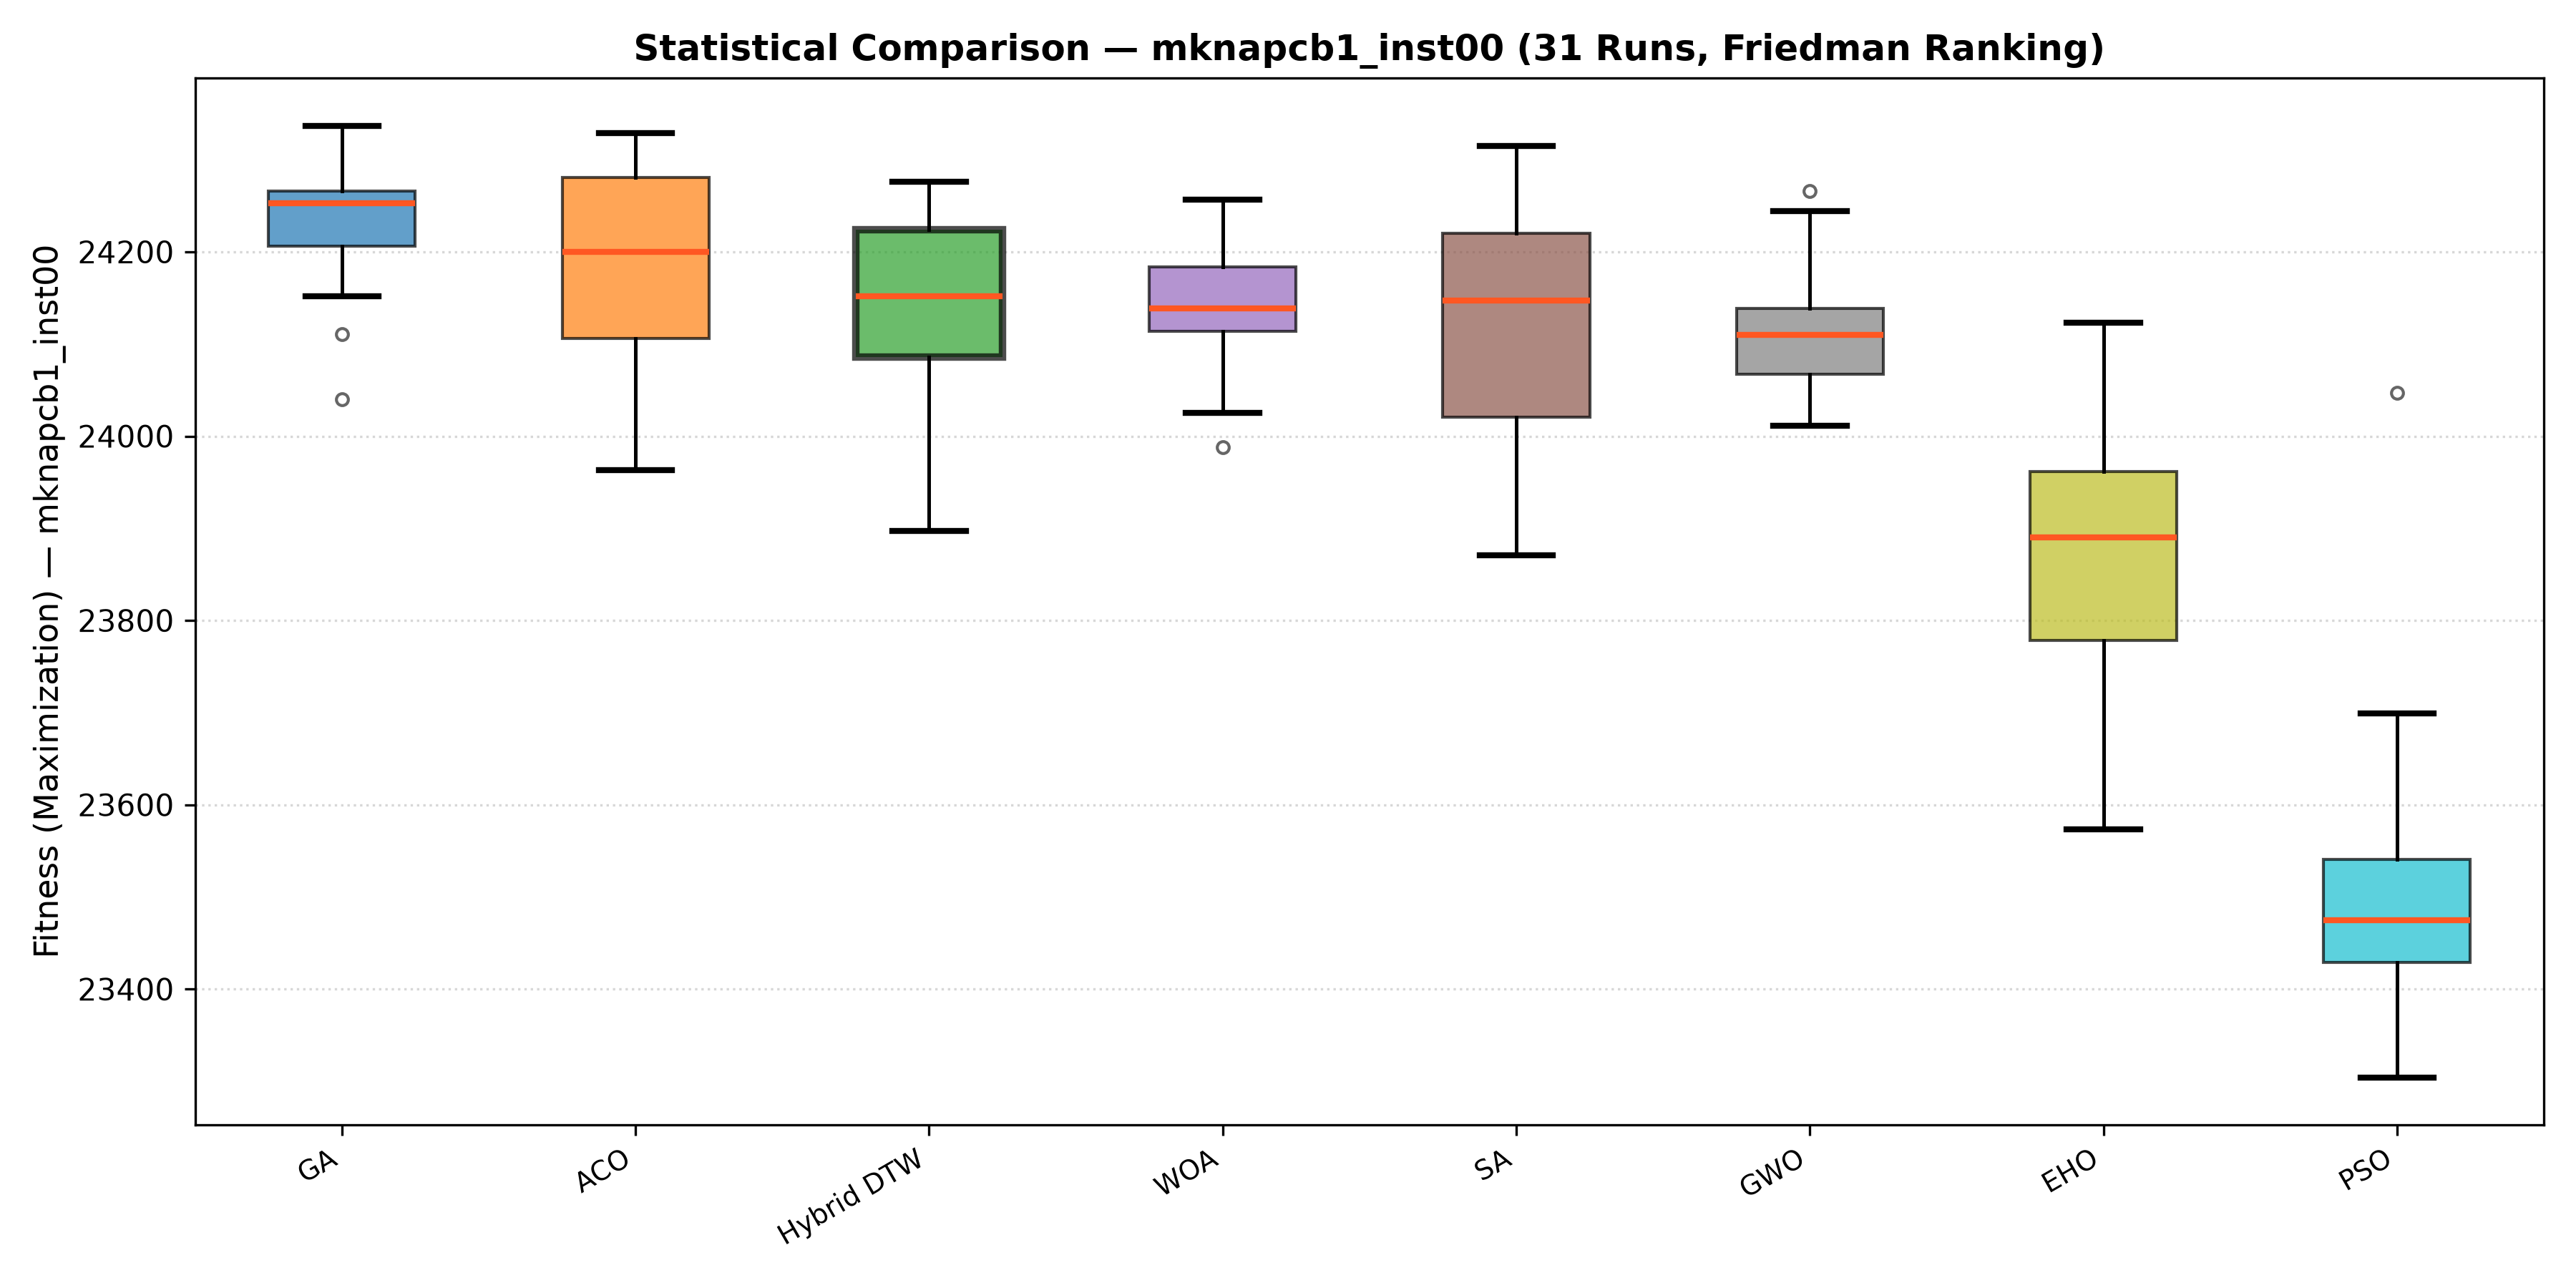
\includegraphics[width=0.32\textwidth]{imagenes_paper/mkp_dtw_3k_mknapcb1_comparativo_mh.png}}\hfill
\subfloat[Best-run convergence.]{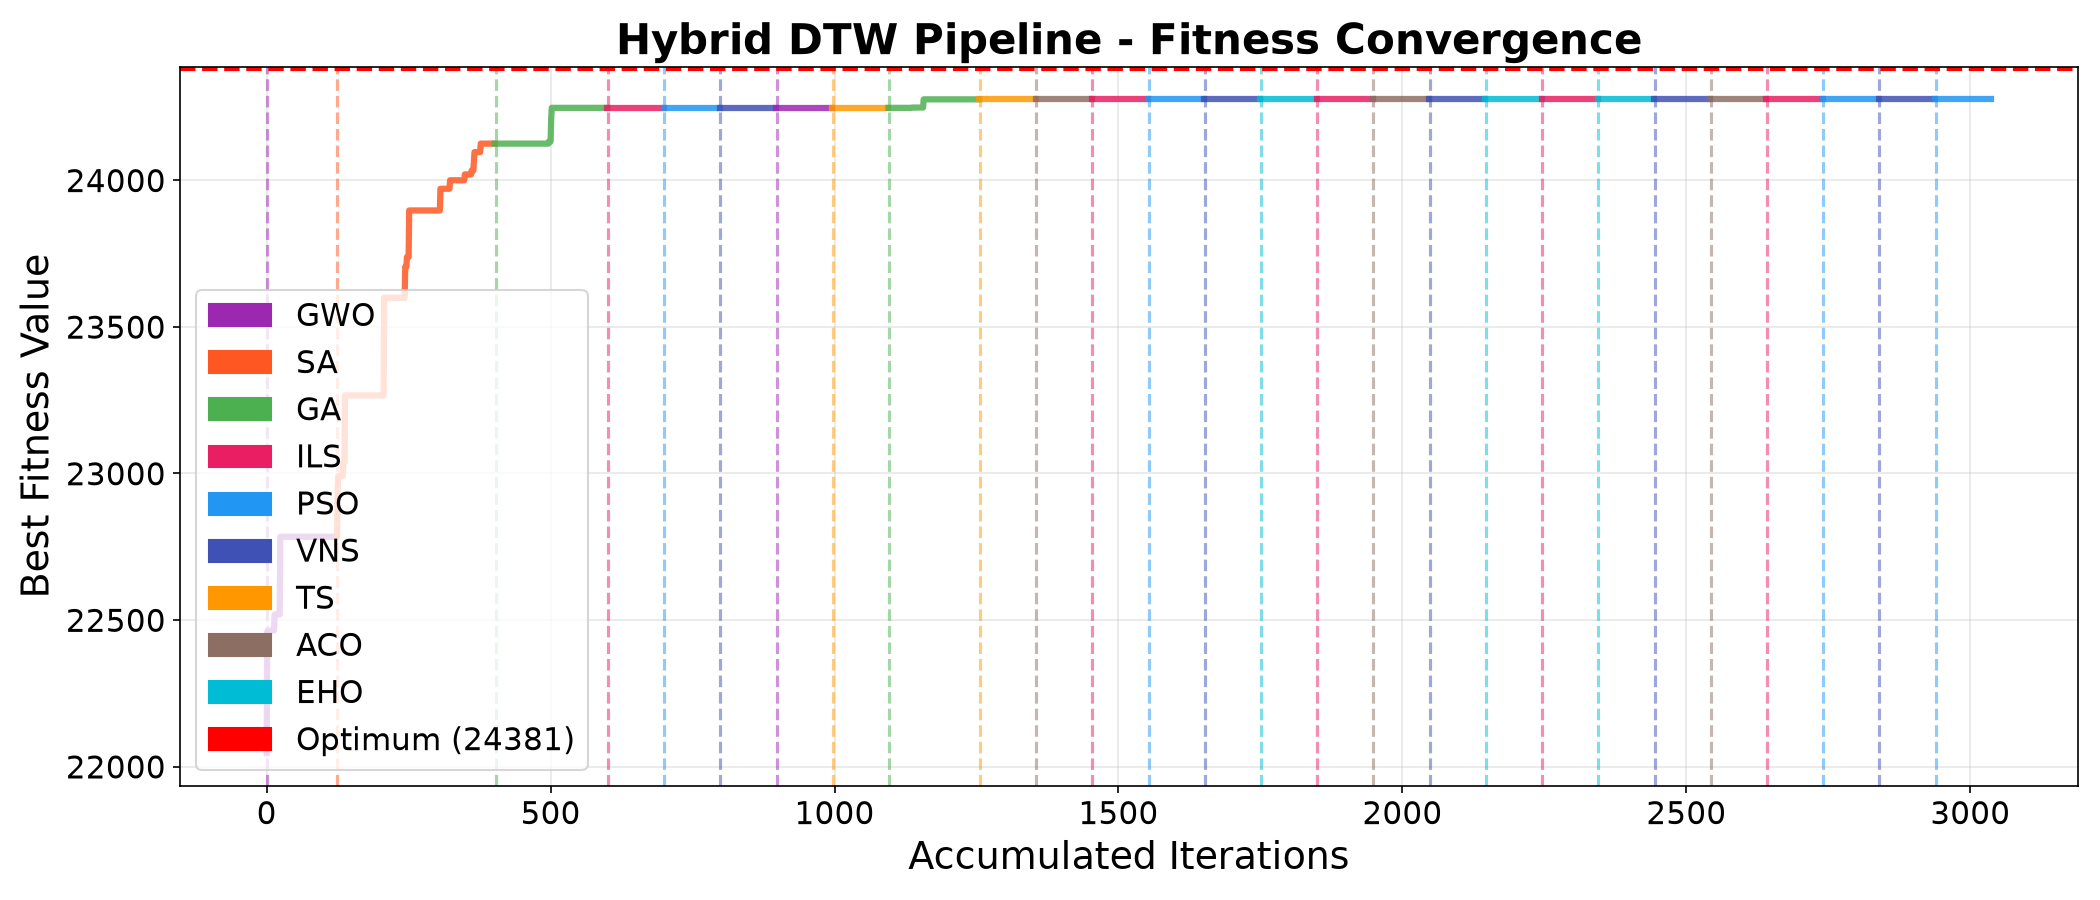
\includegraphics[width=0.32\textwidth]{imagenes_paper/mkp_dtw_3k_mknapcb1_convergencia.png}}\hfill
\subfloat[Elastic metric $\Delta=D_1-D_2$.]{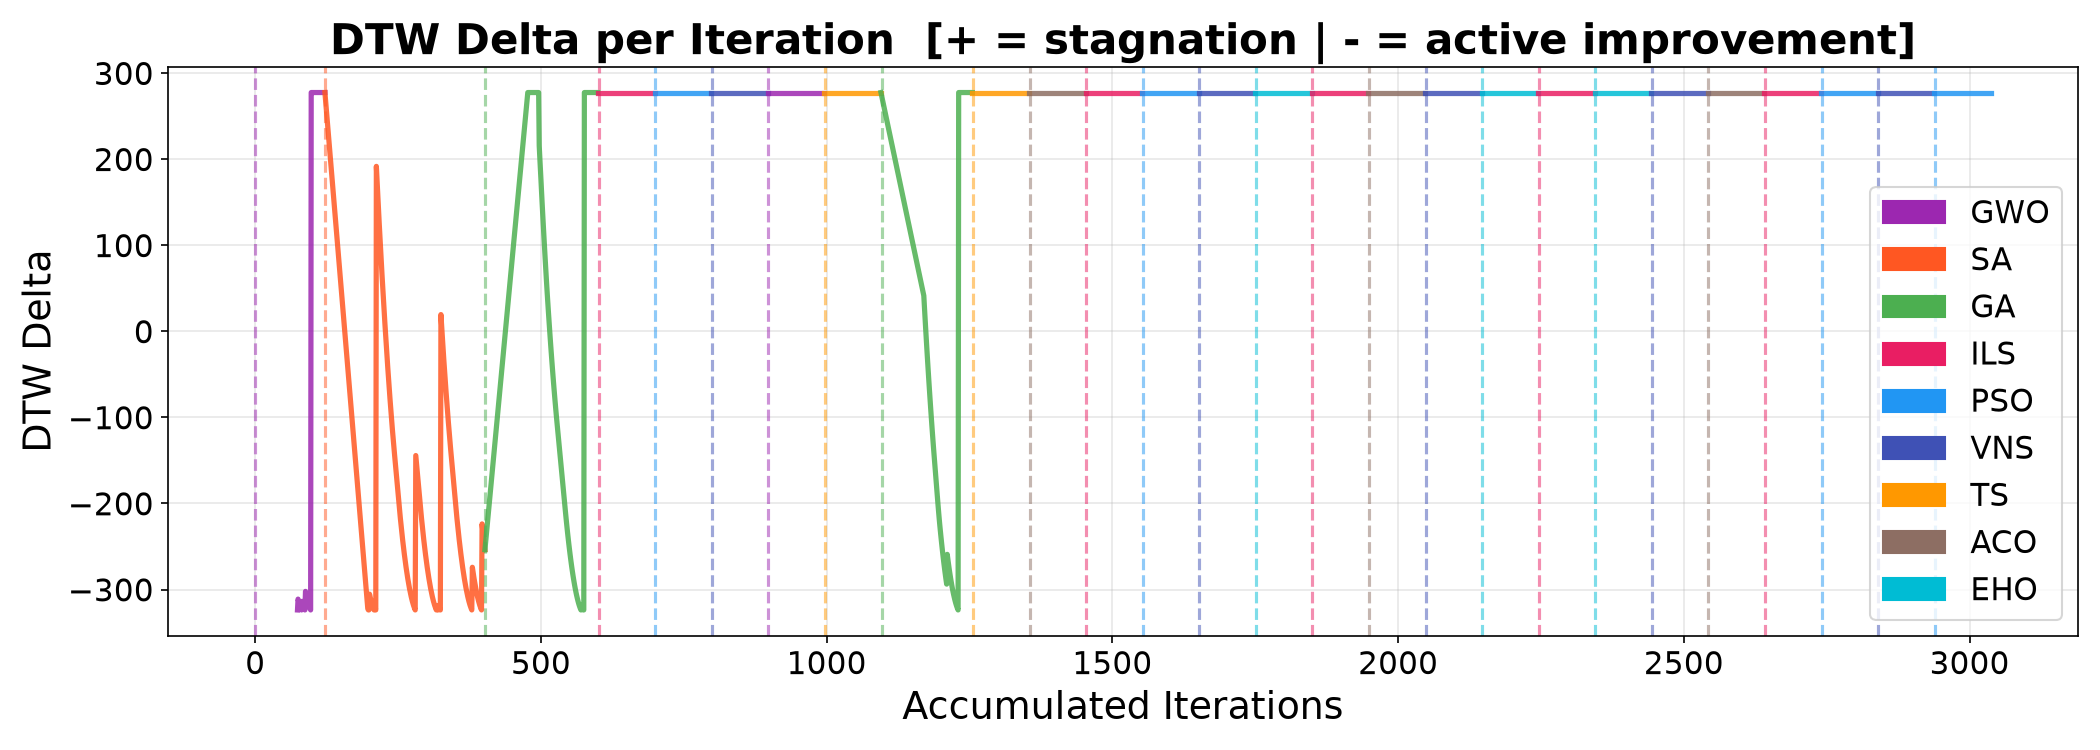
\includegraphics[width=0.32\textwidth]{imagenes_paper/mkp_dtw_3k_mknapcb1_delta.png}}
\caption{Diagnostic suite for instance \textbf{mknapcb1} ($n=100$, $m=5$) under the DTW framework with $T_{\max}=3{,}000$: (a)~final-fitness distribution over $N=31$ runs; (b)~convergence trajectory of the best run; (c)~elastic warping profile $\Delta$.}
\label{fig:mkp-best-cb1}
\end{figure}

% --- mknapcb2: DDTW, 3,000 iterations ---
\begin{figure}[htbp]
\centering
\subfloat[Metaheuristic comparison.]{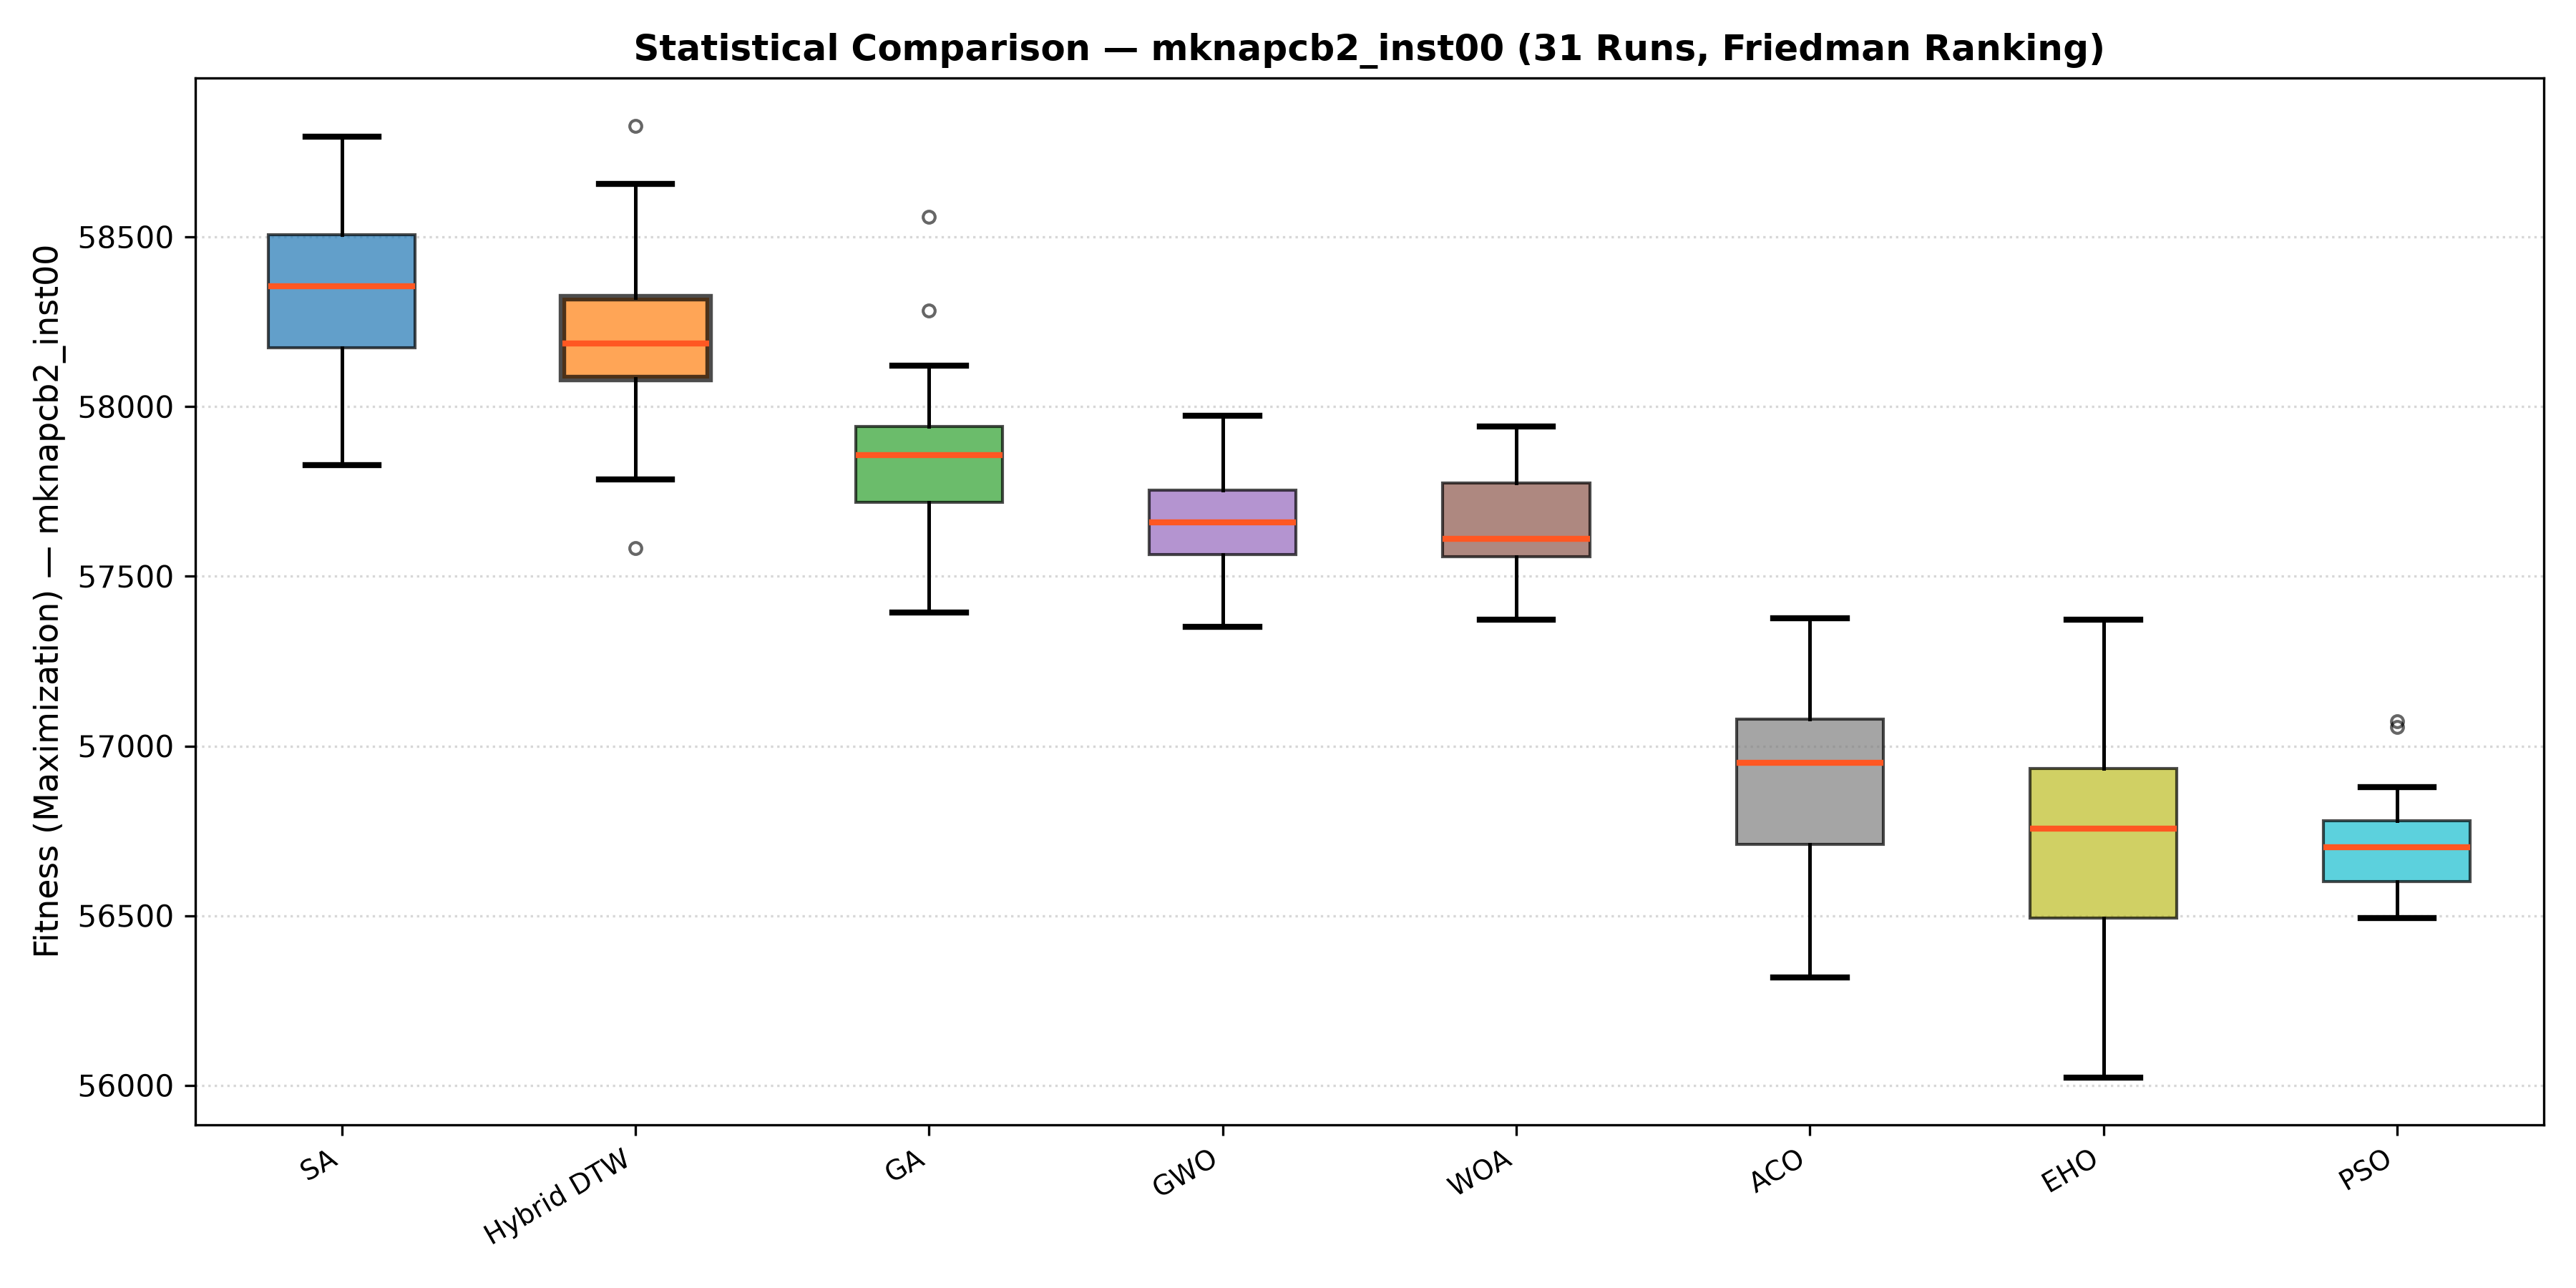
\includegraphics[width=0.32\textwidth]{imagenes_paper/mkp_ddtw_3k_mknapcb2_comparativo_mh.png}}\hfill
\subfloat[Best-run convergence.]{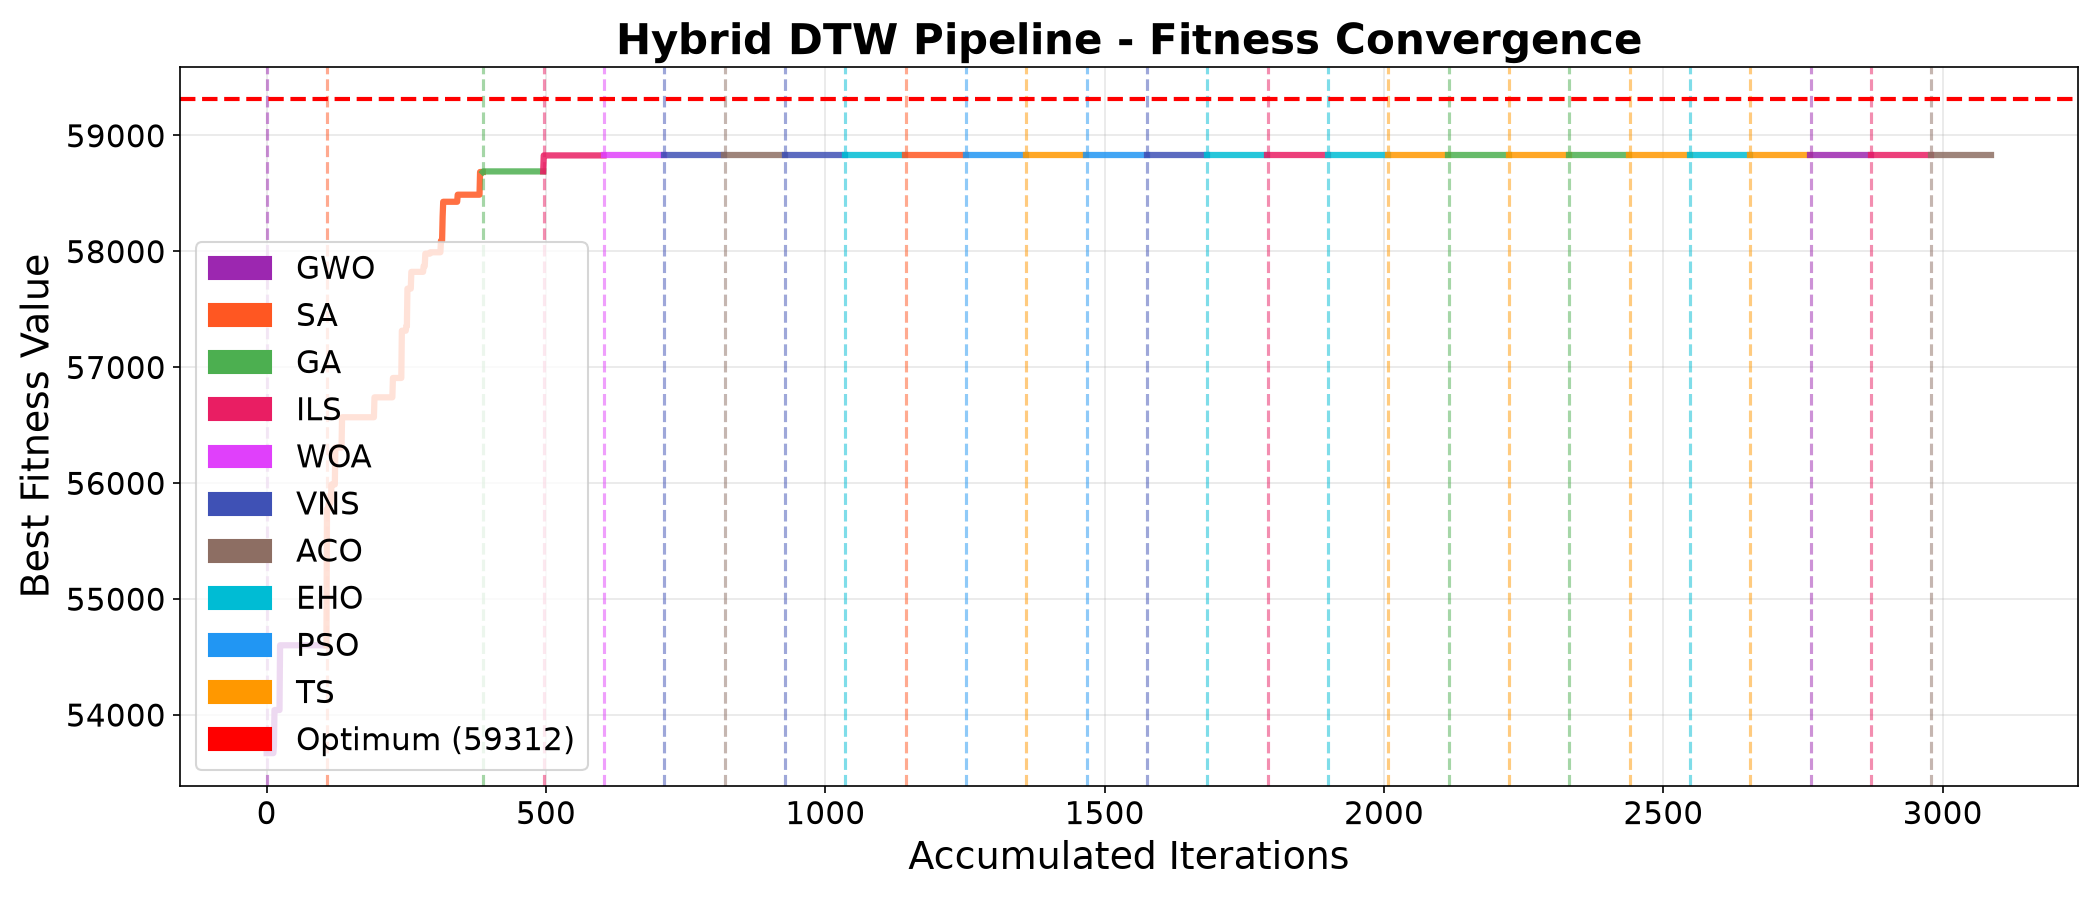
\includegraphics[width=0.32\textwidth]{imagenes_paper/mkp_ddtw_3k_mknapcb2_convergencia.png}}\hfill
\subfloat[Elastic metric $\Delta=D_1-D_2$.]{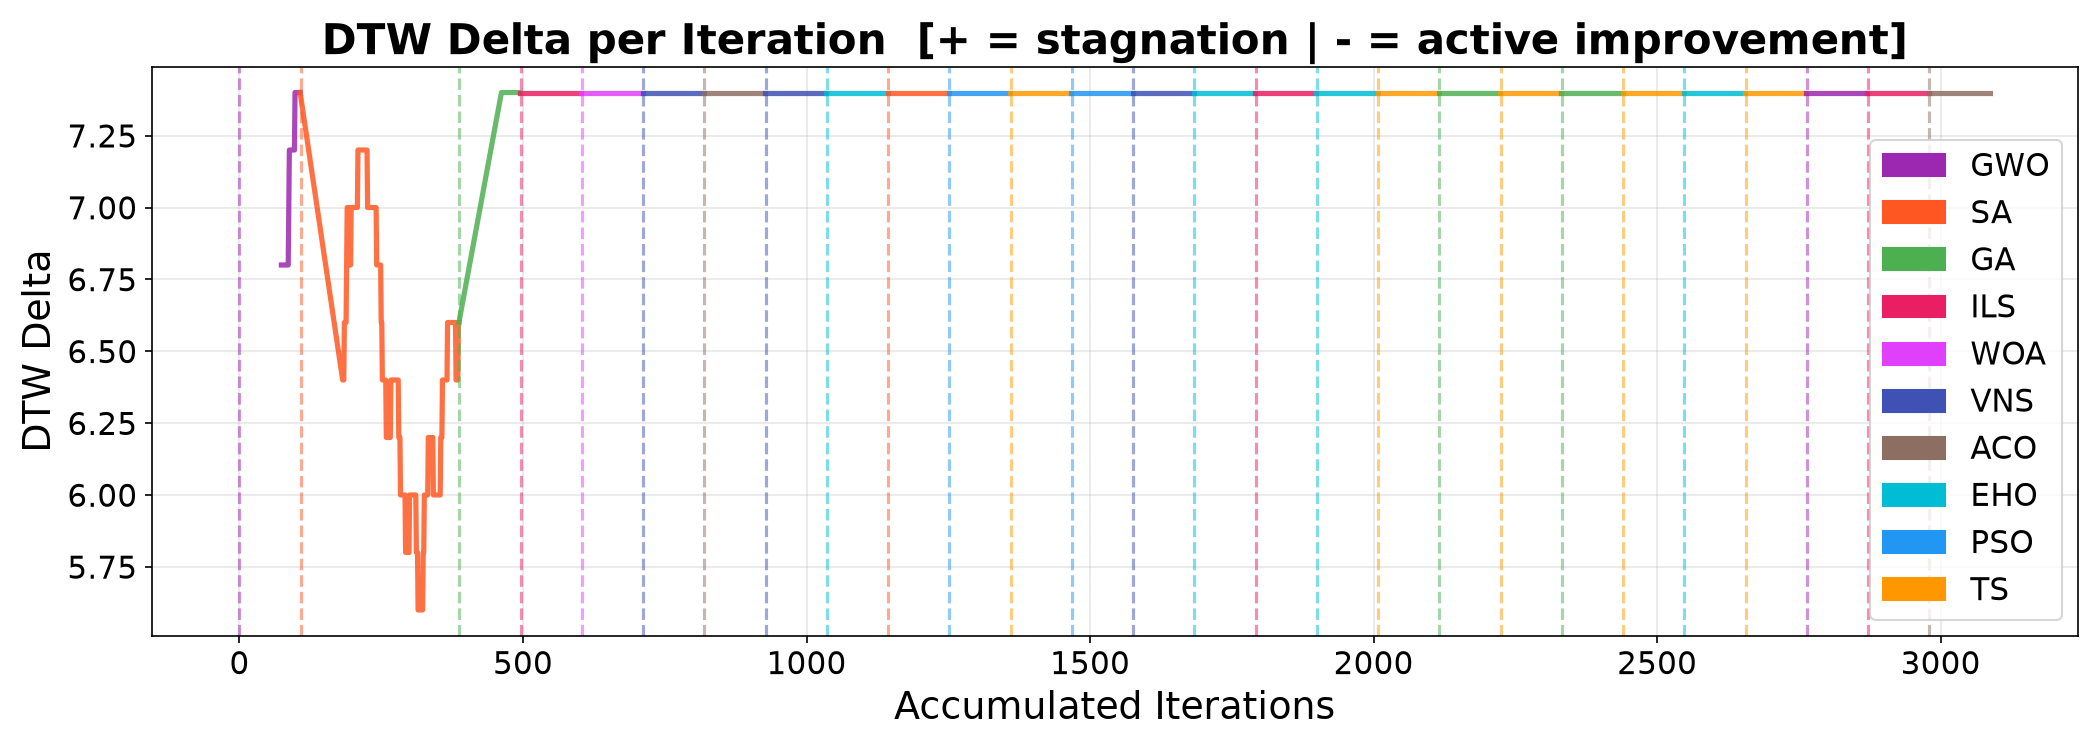
\includegraphics[width=0.32\textwidth]{imagenes_paper/mkp_ddtw_3k_mknapcb2_delta.png}}
\caption{Diagnostic suite for instance \textbf{mknapcb2} ($n=250$, $m=5$) under the DDTW framework with $T_{\max}=3{,}000$: (a)~final-fitness distribution over $N=31$ runs; (b)~convergence trajectory of the best run; (c)~elastic warping profile $\Delta$.}
\label{fig:mkp-best-cb2}
\end{figure}

% --- mknapcb3: DTW, 3,000 iterations ---
\begin{figure}[htbp]
\centering
\subfloat[Metaheuristic comparison.]{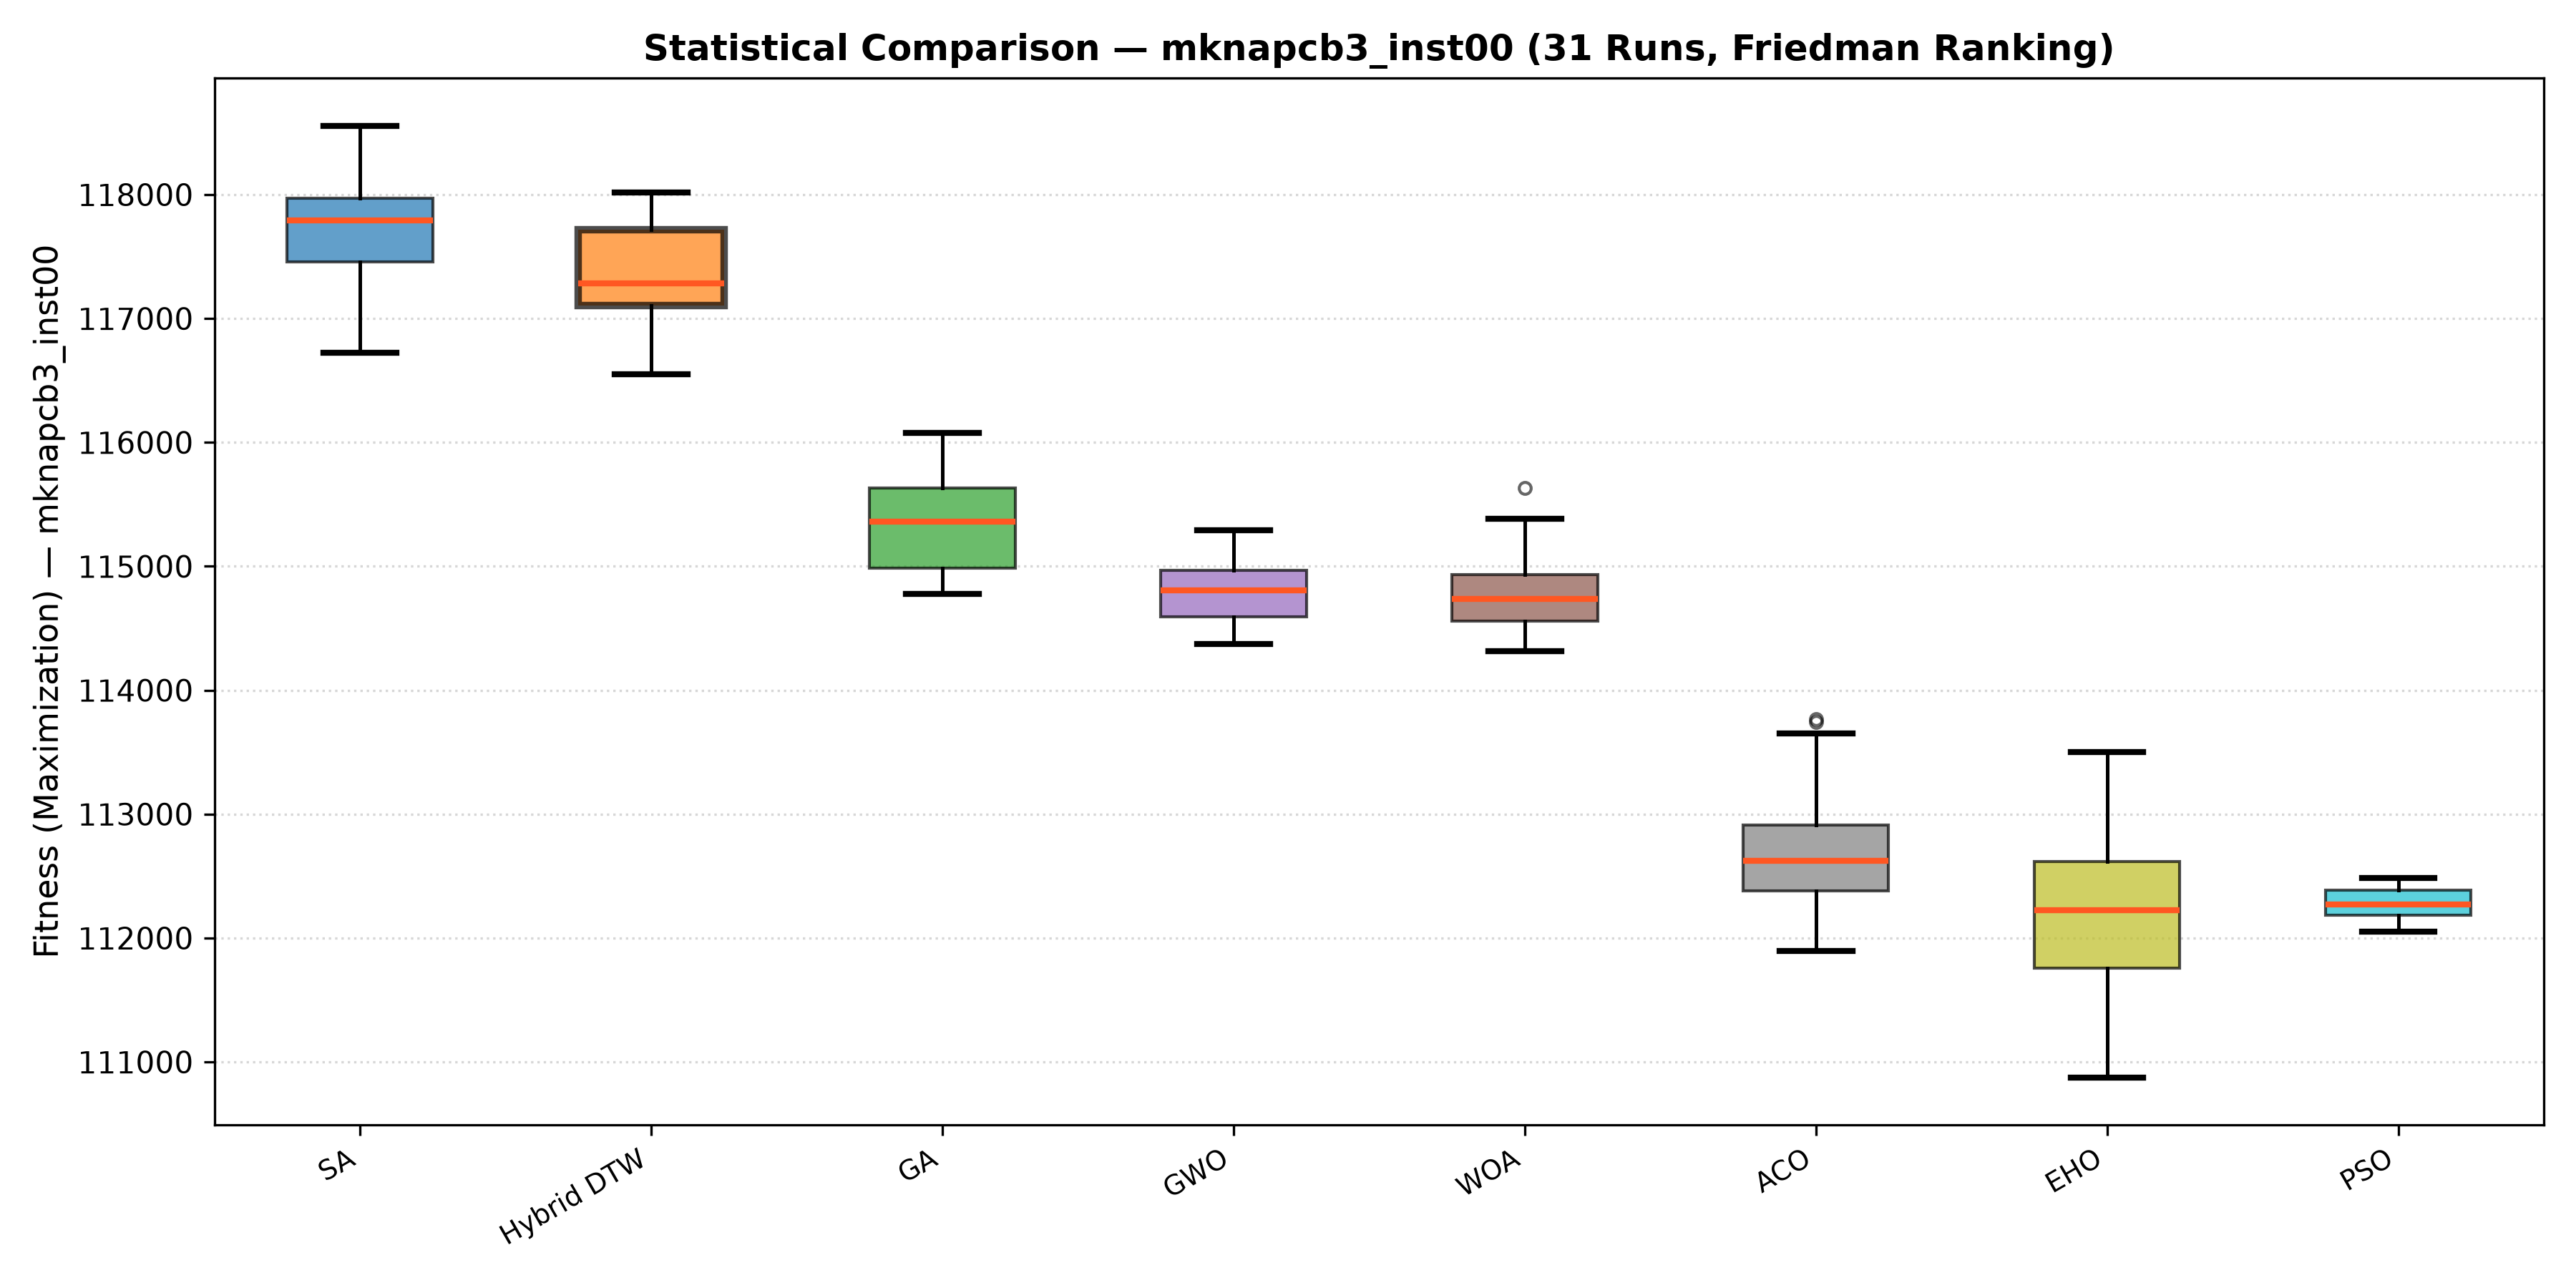
\includegraphics[width=0.32\textwidth]{imagenes_paper/mkp_dtw_3k_mknapcb3_comparativo_mh.png}}\hfill
\subfloat[Best-run convergence.]{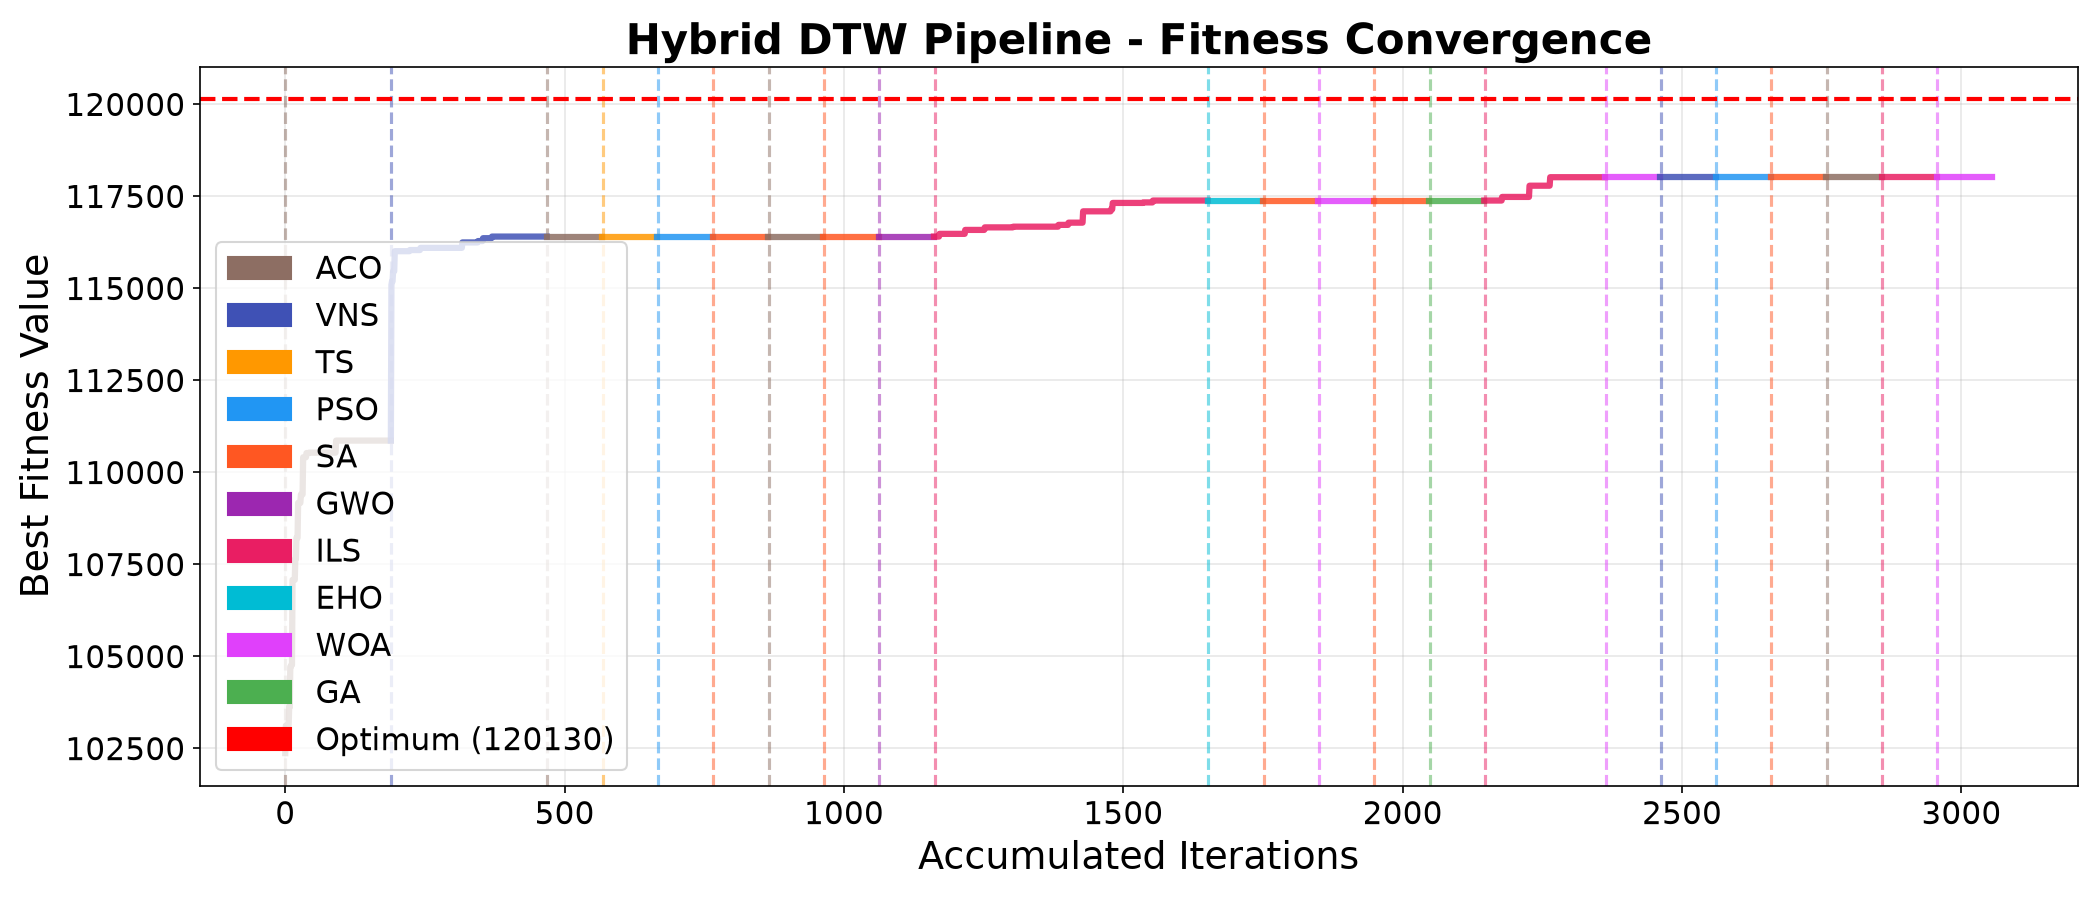
\includegraphics[width=0.32\textwidth]{imagenes_paper/mkp_dtw_3k_mknapcb3_convergencia.png}}\hfill
\subfloat[Elastic metric $\Delta=D_1-D_2$.]{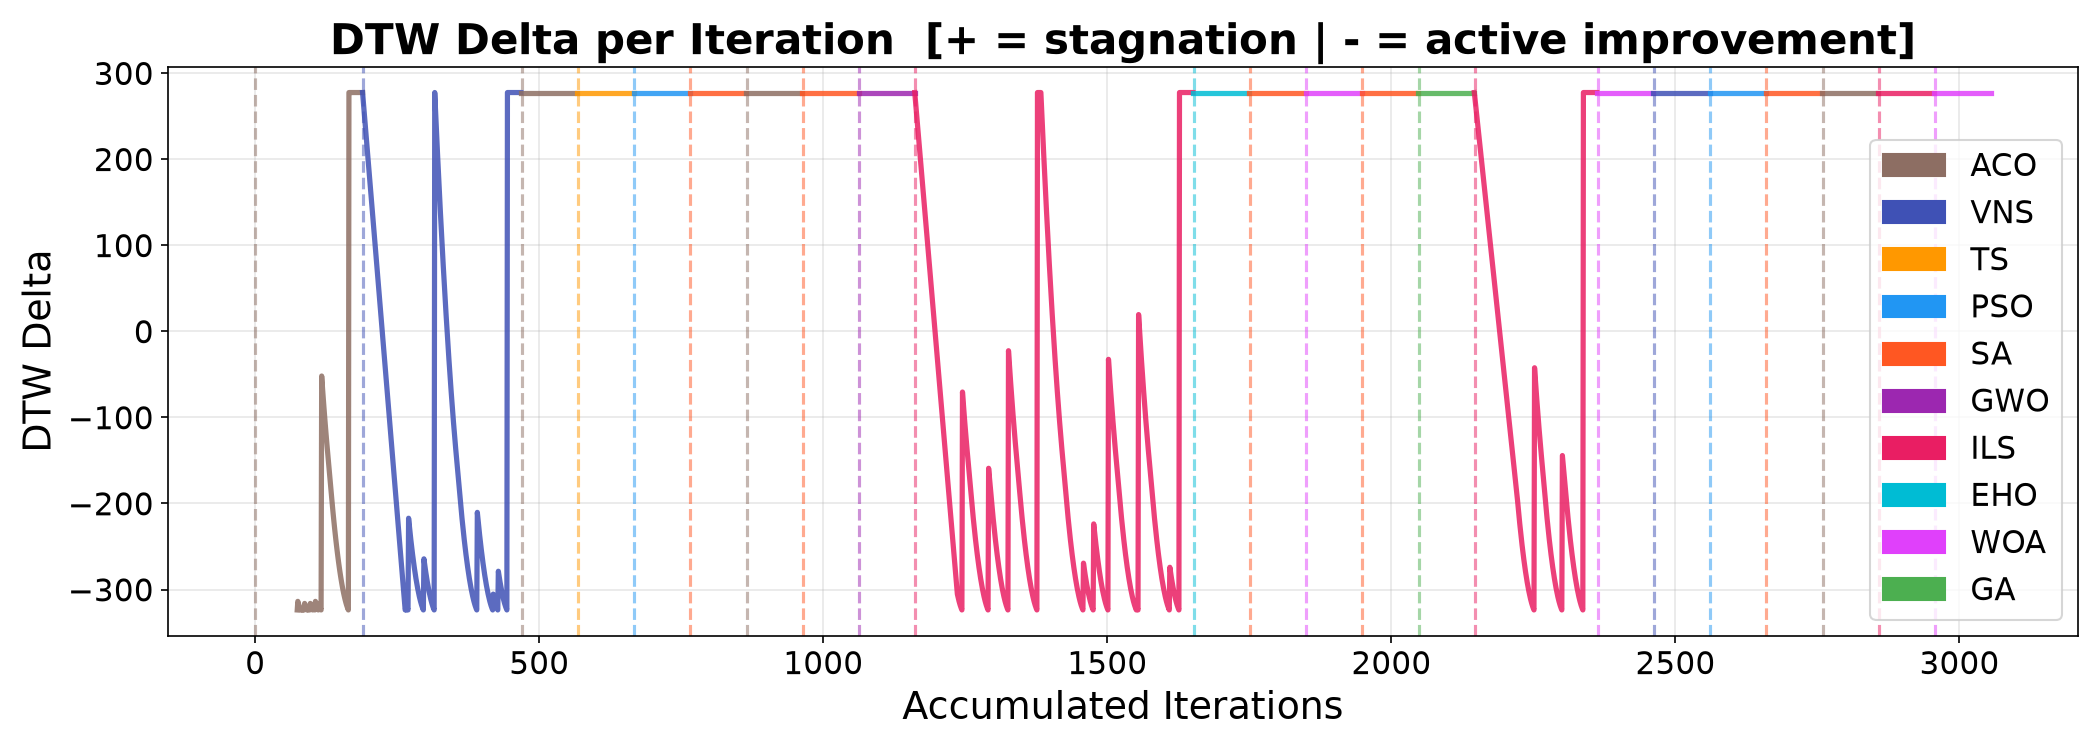
\includegraphics[width=0.32\textwidth]{imagenes_paper/mkp_dtw_3k_mknapcb3_delta.png}}
\caption{Diagnostic suite for instance \textbf{mknapcb3} ($n=500$, $m=5$) under the DTW framework with $T_{\max}=3{,}000$: (a)~final-fitness distribution over $N=31$ runs; (b)~convergence trajectory of the best run; (c)~elastic warping profile $\Delta$.}
\label{fig:mkp-best-cb3}
\end{figure}

% --- mknapcb4: DTW, 3,000 iterations ---
\begin{figure}[htbp]
\centering
\subfloat[Metaheuristic comparison.]{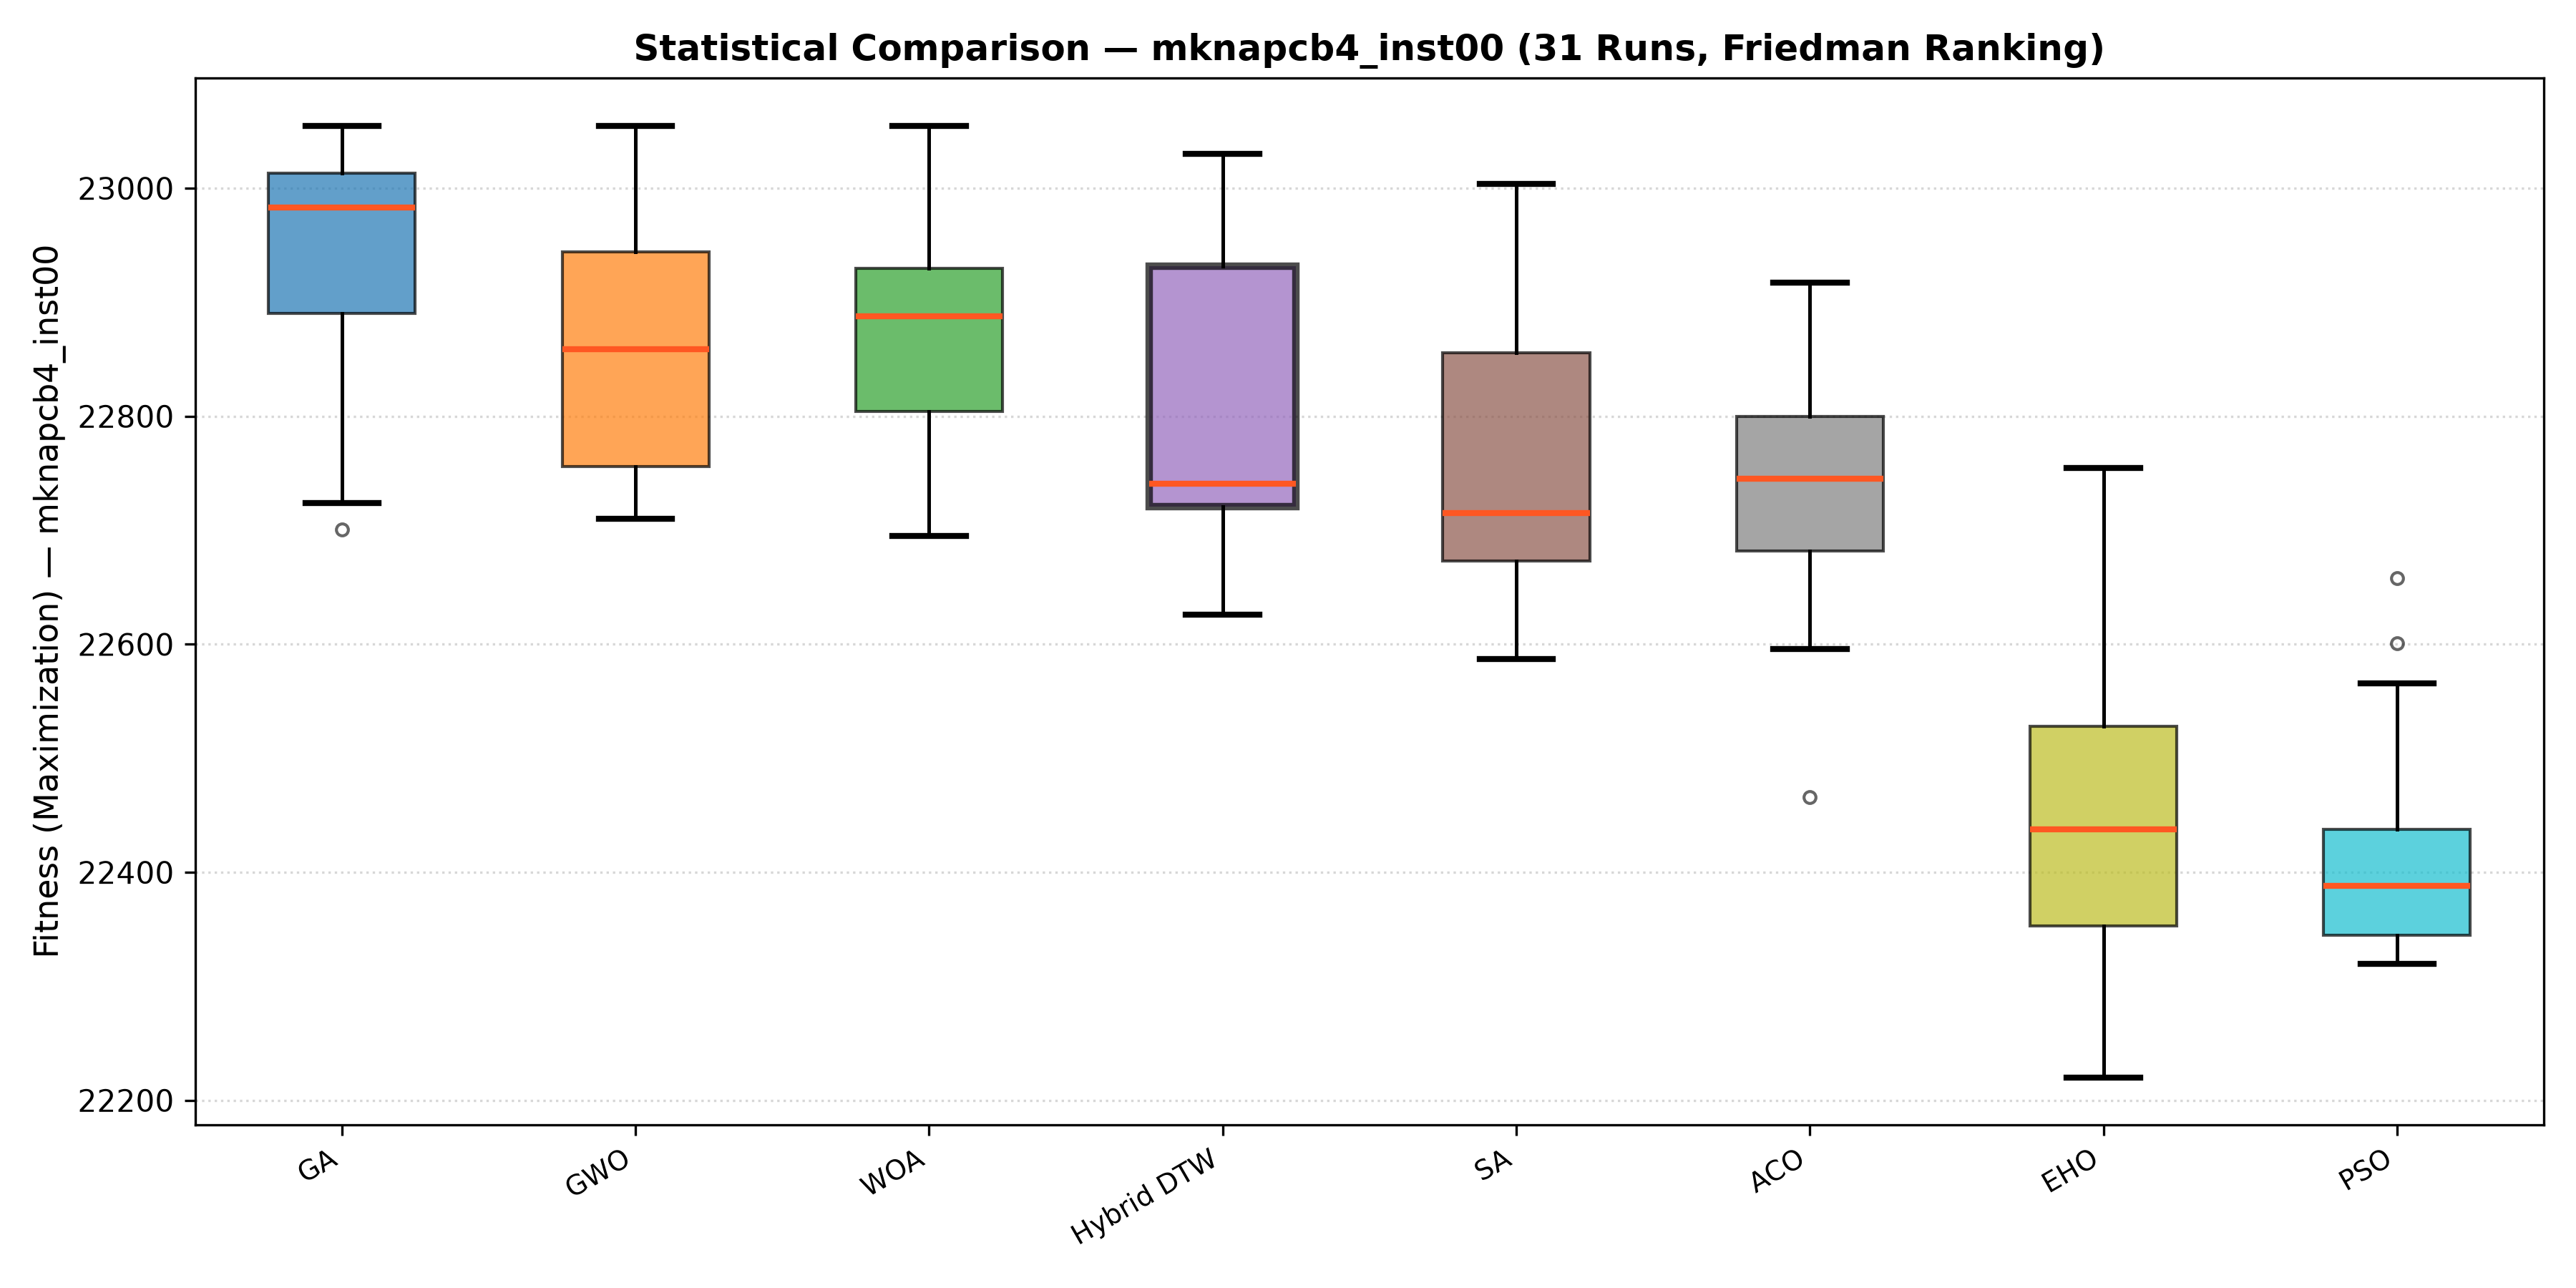
\includegraphics[width=0.32\textwidth]{imagenes_paper/mkp_dtw_3k_mknapcb4_comparativo_mh.png}}\hfill
\subfloat[Best-run convergence.]{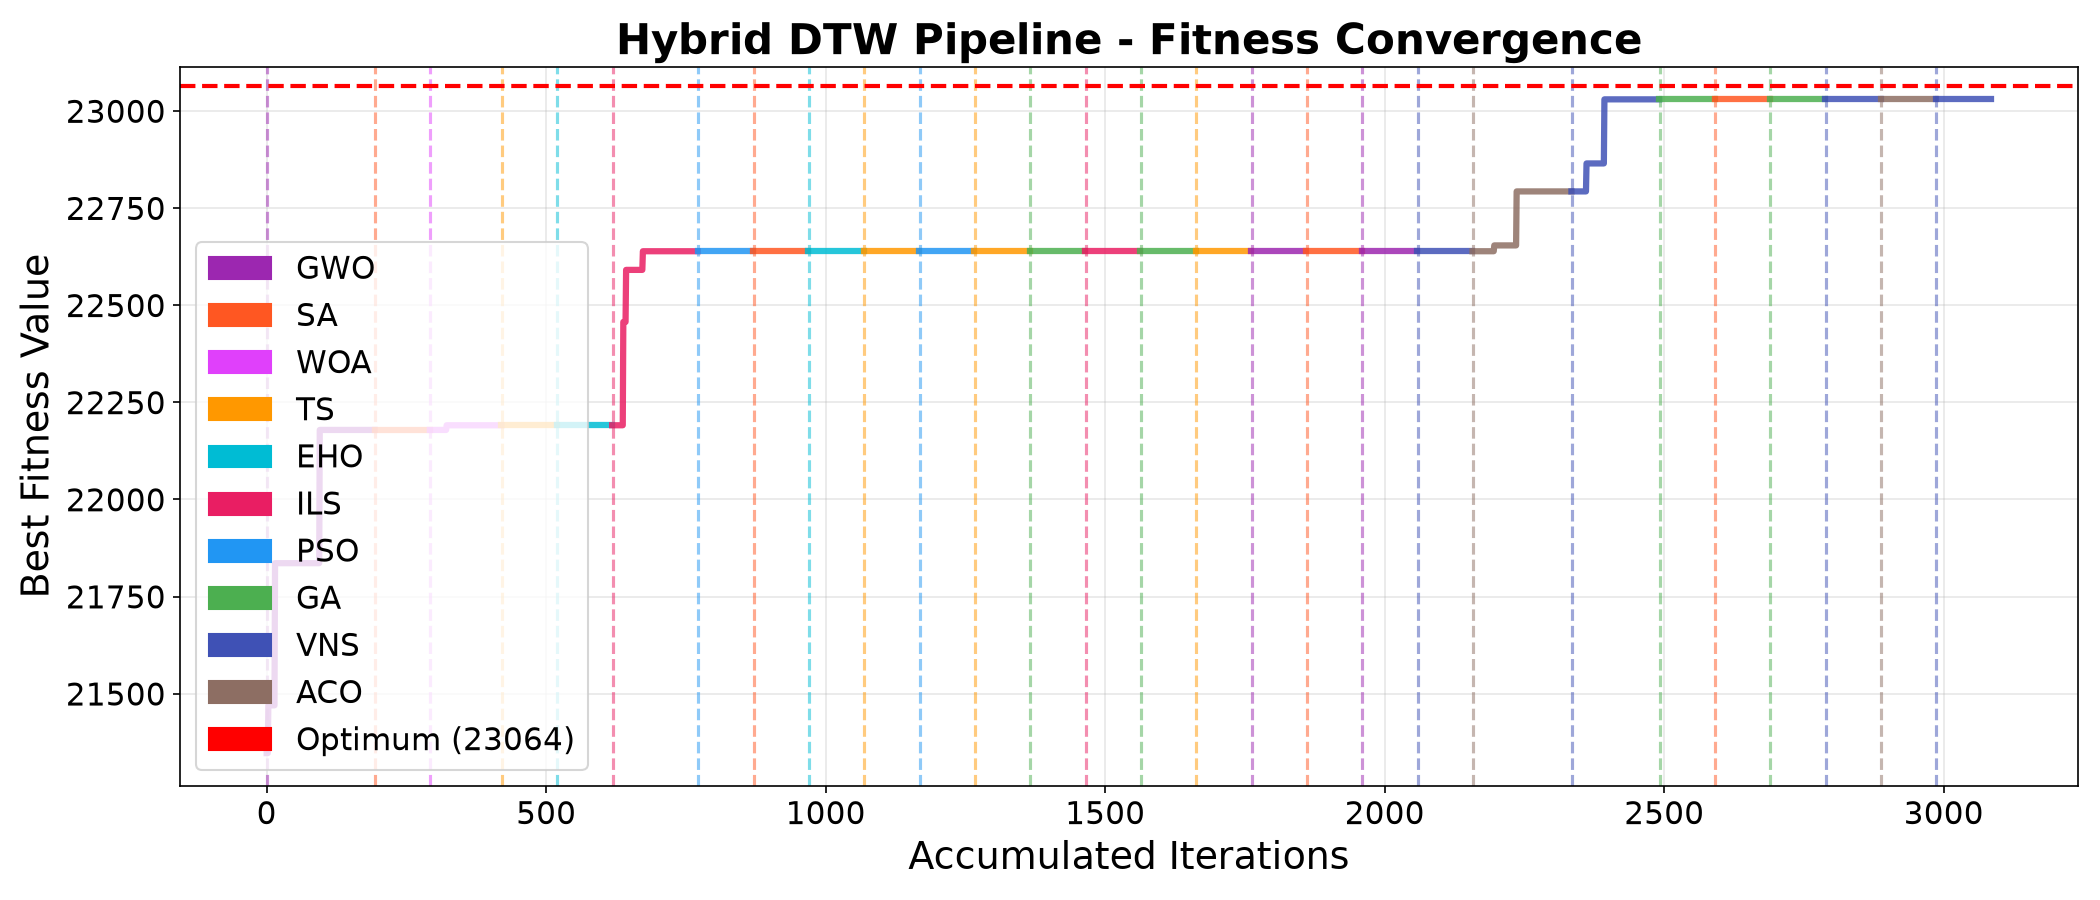
\includegraphics[width=0.32\textwidth]{imagenes_paper/mkp_dtw_3k_mknapcb4_convergencia.png}}\hfill
\subfloat[Elastic metric $\Delta=D_1-D_2$.]{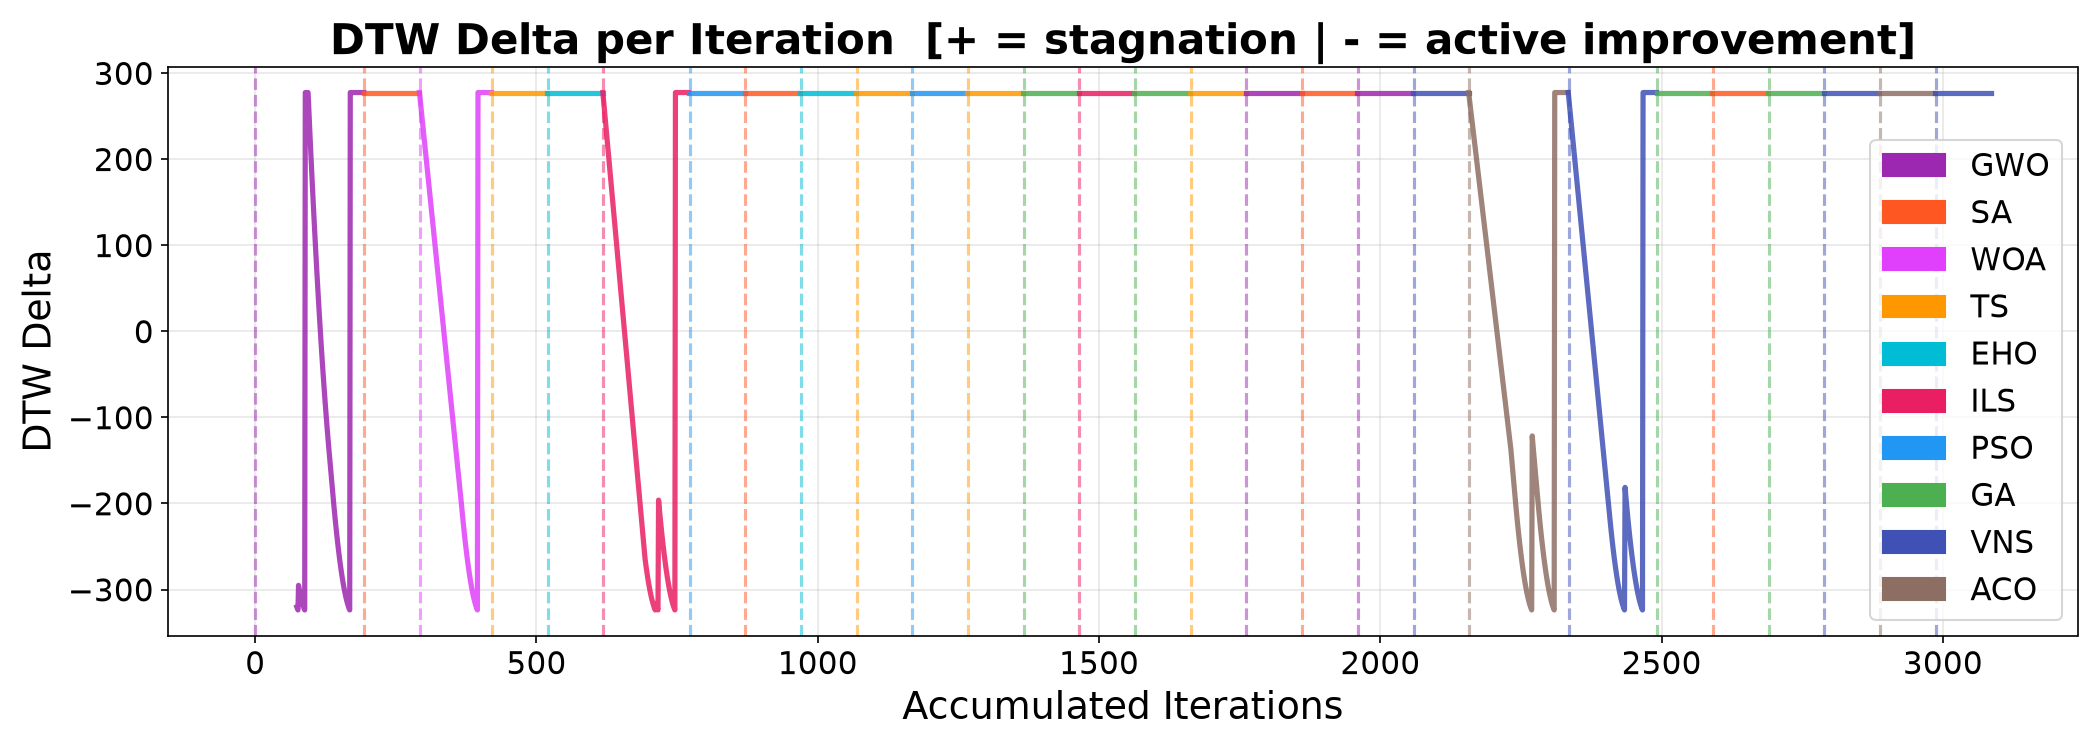
\includegraphics[width=0.32\textwidth]{imagenes_paper/mkp_dtw_3k_mknapcb4_delta.png}}
\caption{Diagnostic suite for instance \textbf{mknapcb4} ($n=100$, $m=10$) under the DTW framework with $T_{\max}=3{,}000$: (a)~final-fitness distribution over $N=31$ runs; (b)~convergence trajectory of the best run; (c)~elastic warping profile $\Delta$.}
\label{fig:mkp-best-cb4}
\end{figure}

% --- mknapcb5: DTW, 3,000 iterations ---
\begin{figure}[htbp]
\centering
\subfloat[Metaheuristic comparison.]{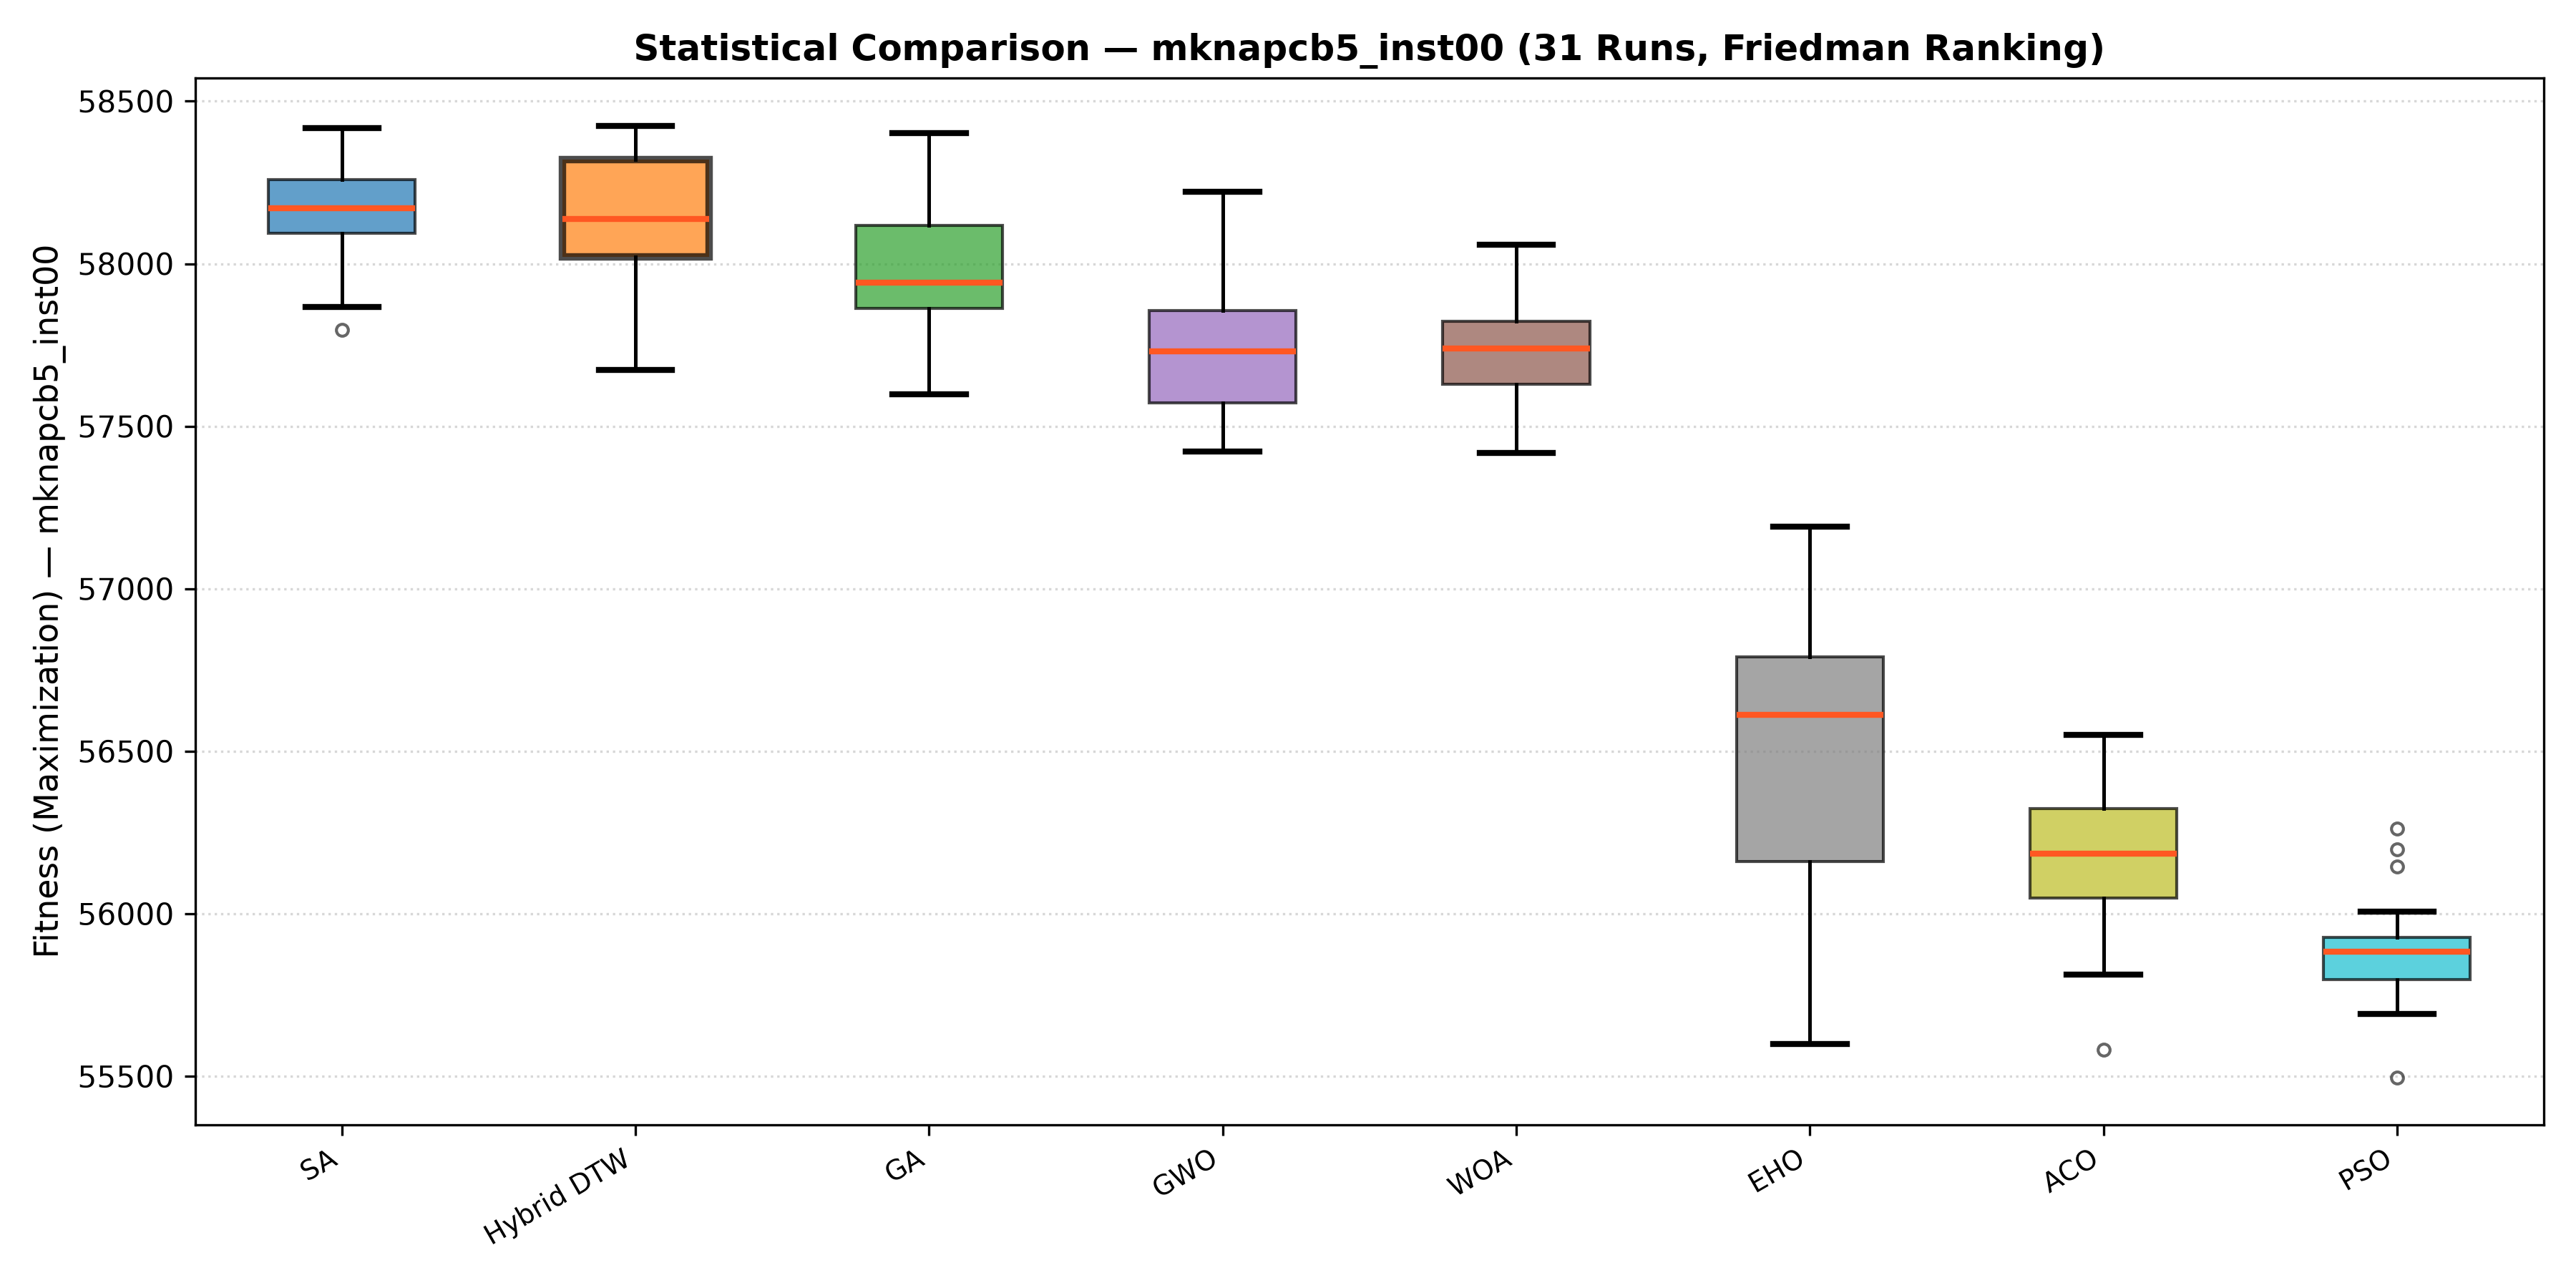
\includegraphics[width=0.32\textwidth]{imagenes_paper/mkp_dtw_3k_mknapcb5_comparativo_mh.png}}\hfill
\subfloat[Best-run convergence.]{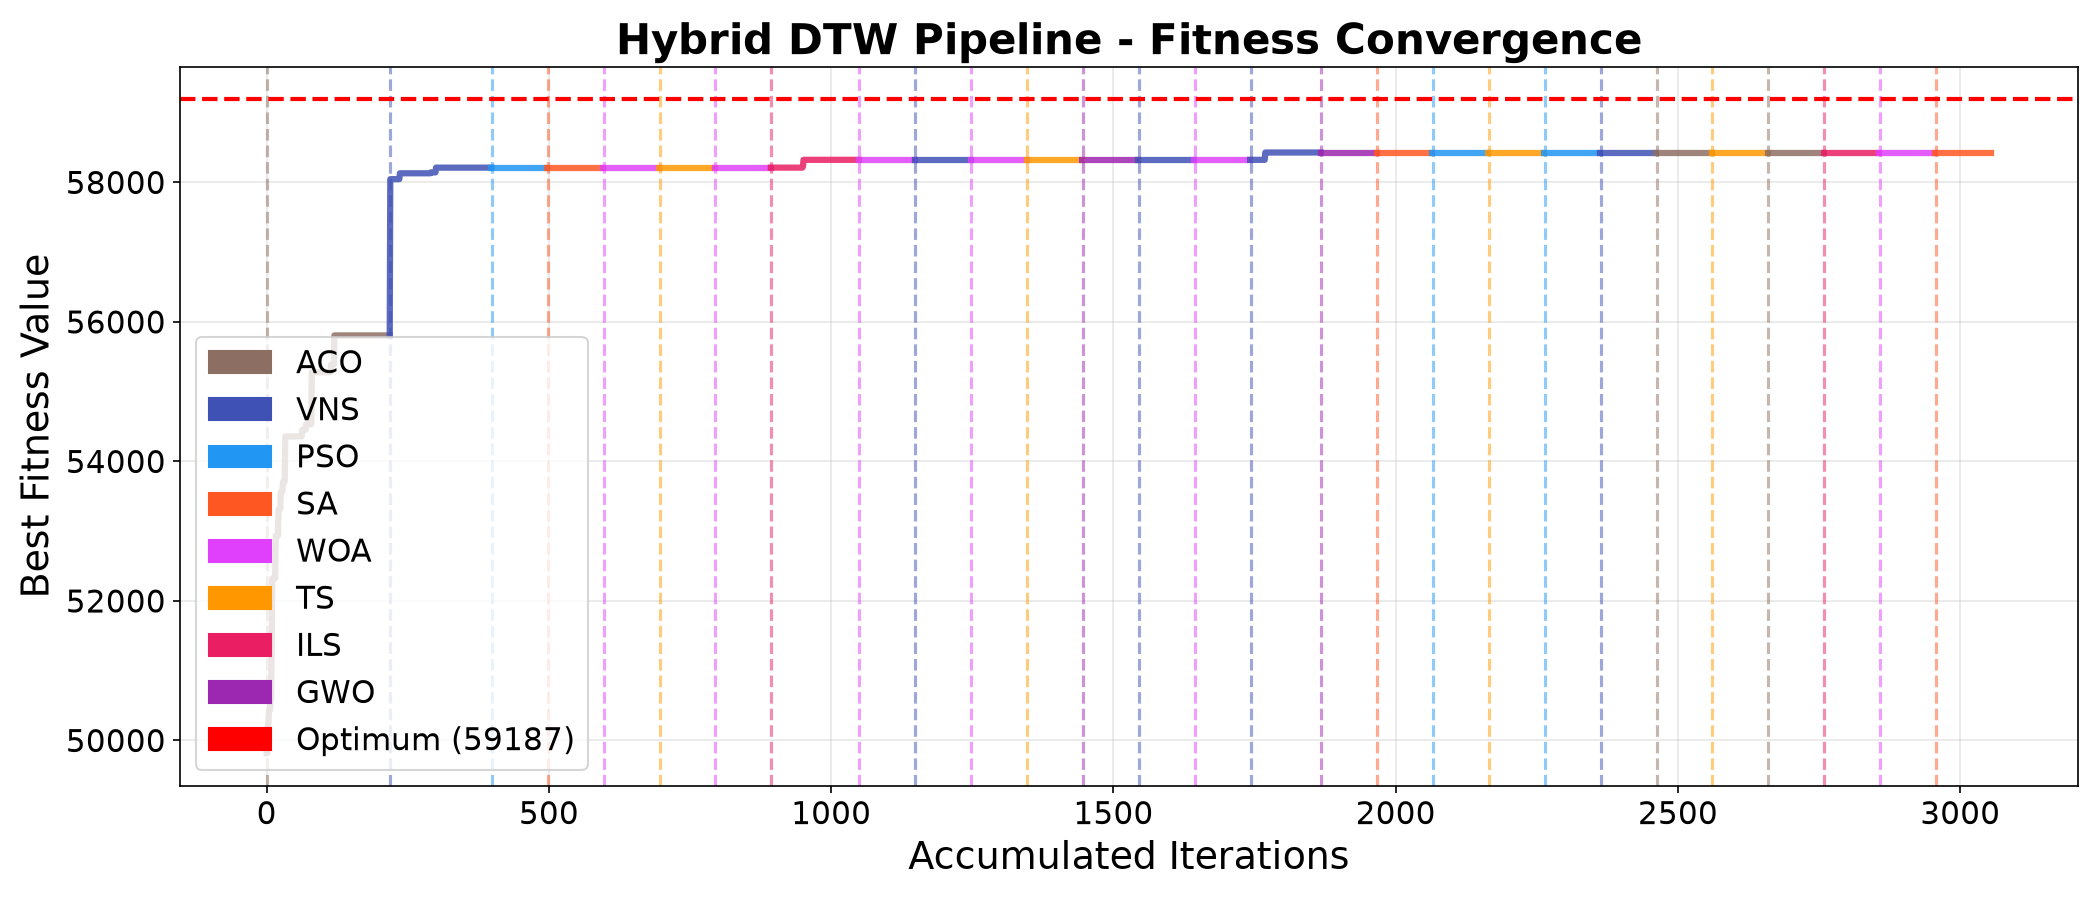
\includegraphics[width=0.32\textwidth]{imagenes_paper/mkp_dtw_3k_mknapcb5_convergencia.png}}\hfill
\subfloat[Elastic metric $\Delta=D_1-D_2$.]{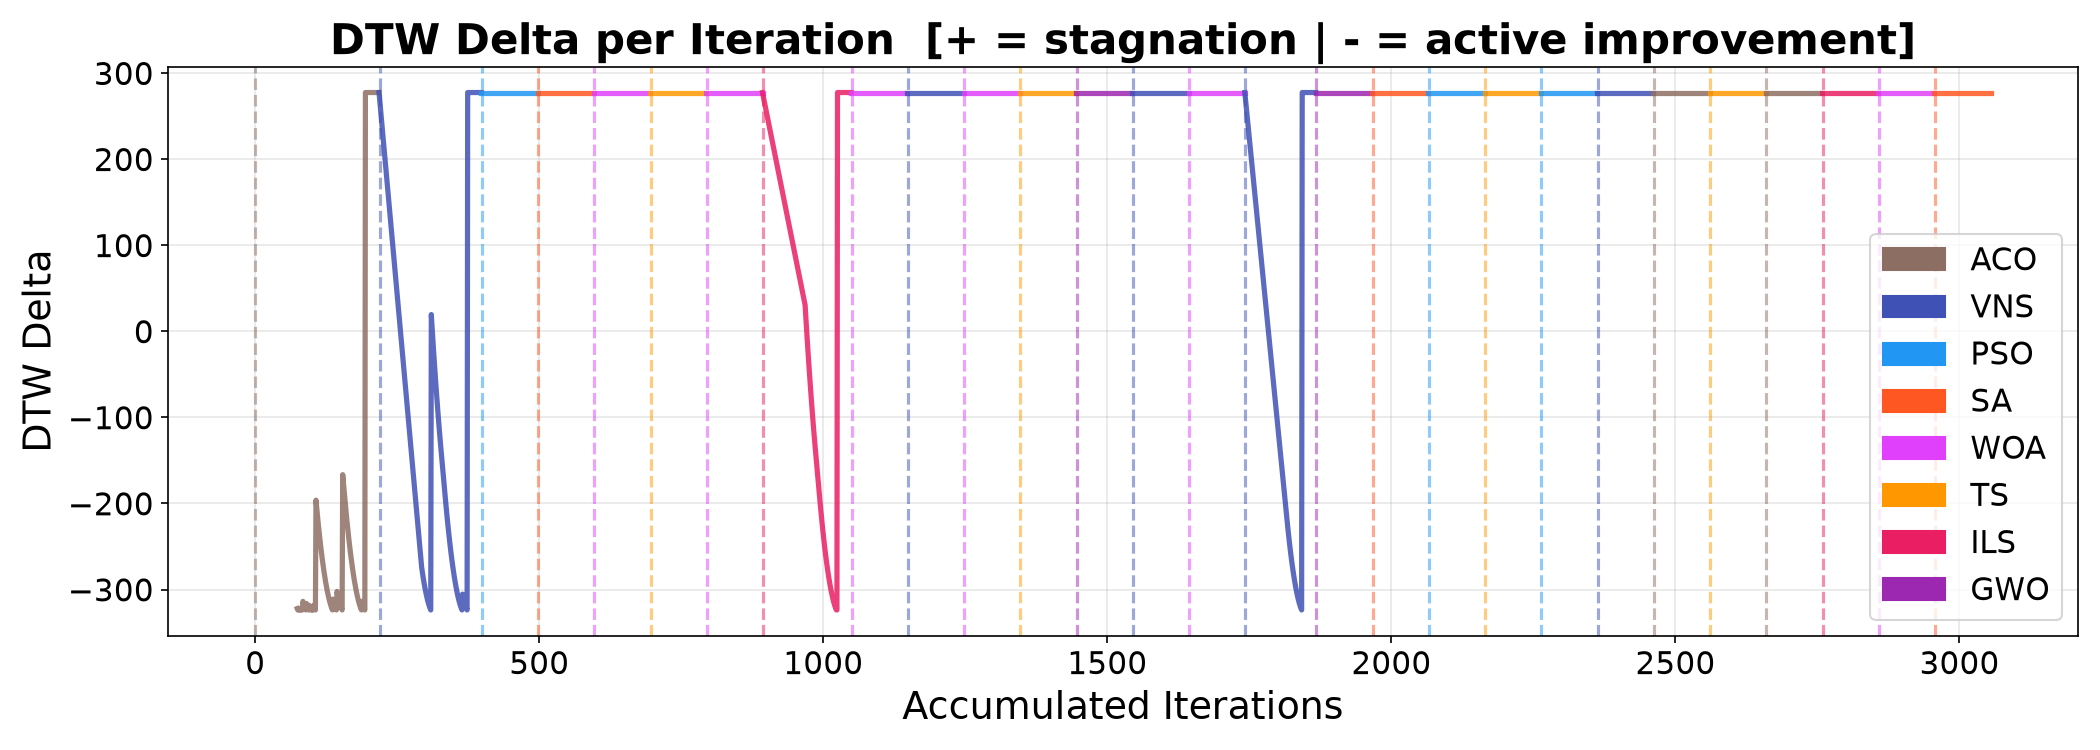
\includegraphics[width=0.32\textwidth]{imagenes_paper/mkp_dtw_3k_mknapcb5_delta.png}}
\caption{Diagnostic suite for instance \textbf{mknapcb5} ($n=250$, $m=10$) under the DTW framework with $T_{\max}=3{,}000$: (a)~final-fitness distribution over $N=31$ runs; (b)~convergence trajectory of the best run; (c)~elastic warping profile $\Delta$.}
\label{fig:mkp-best-cb5}
\end{figure}

% --- mknapcb6: DTW, 3,000 iterations ---
\begin{figure}[htbp]
\centering
\subfloat[Metaheuristic comparison.]{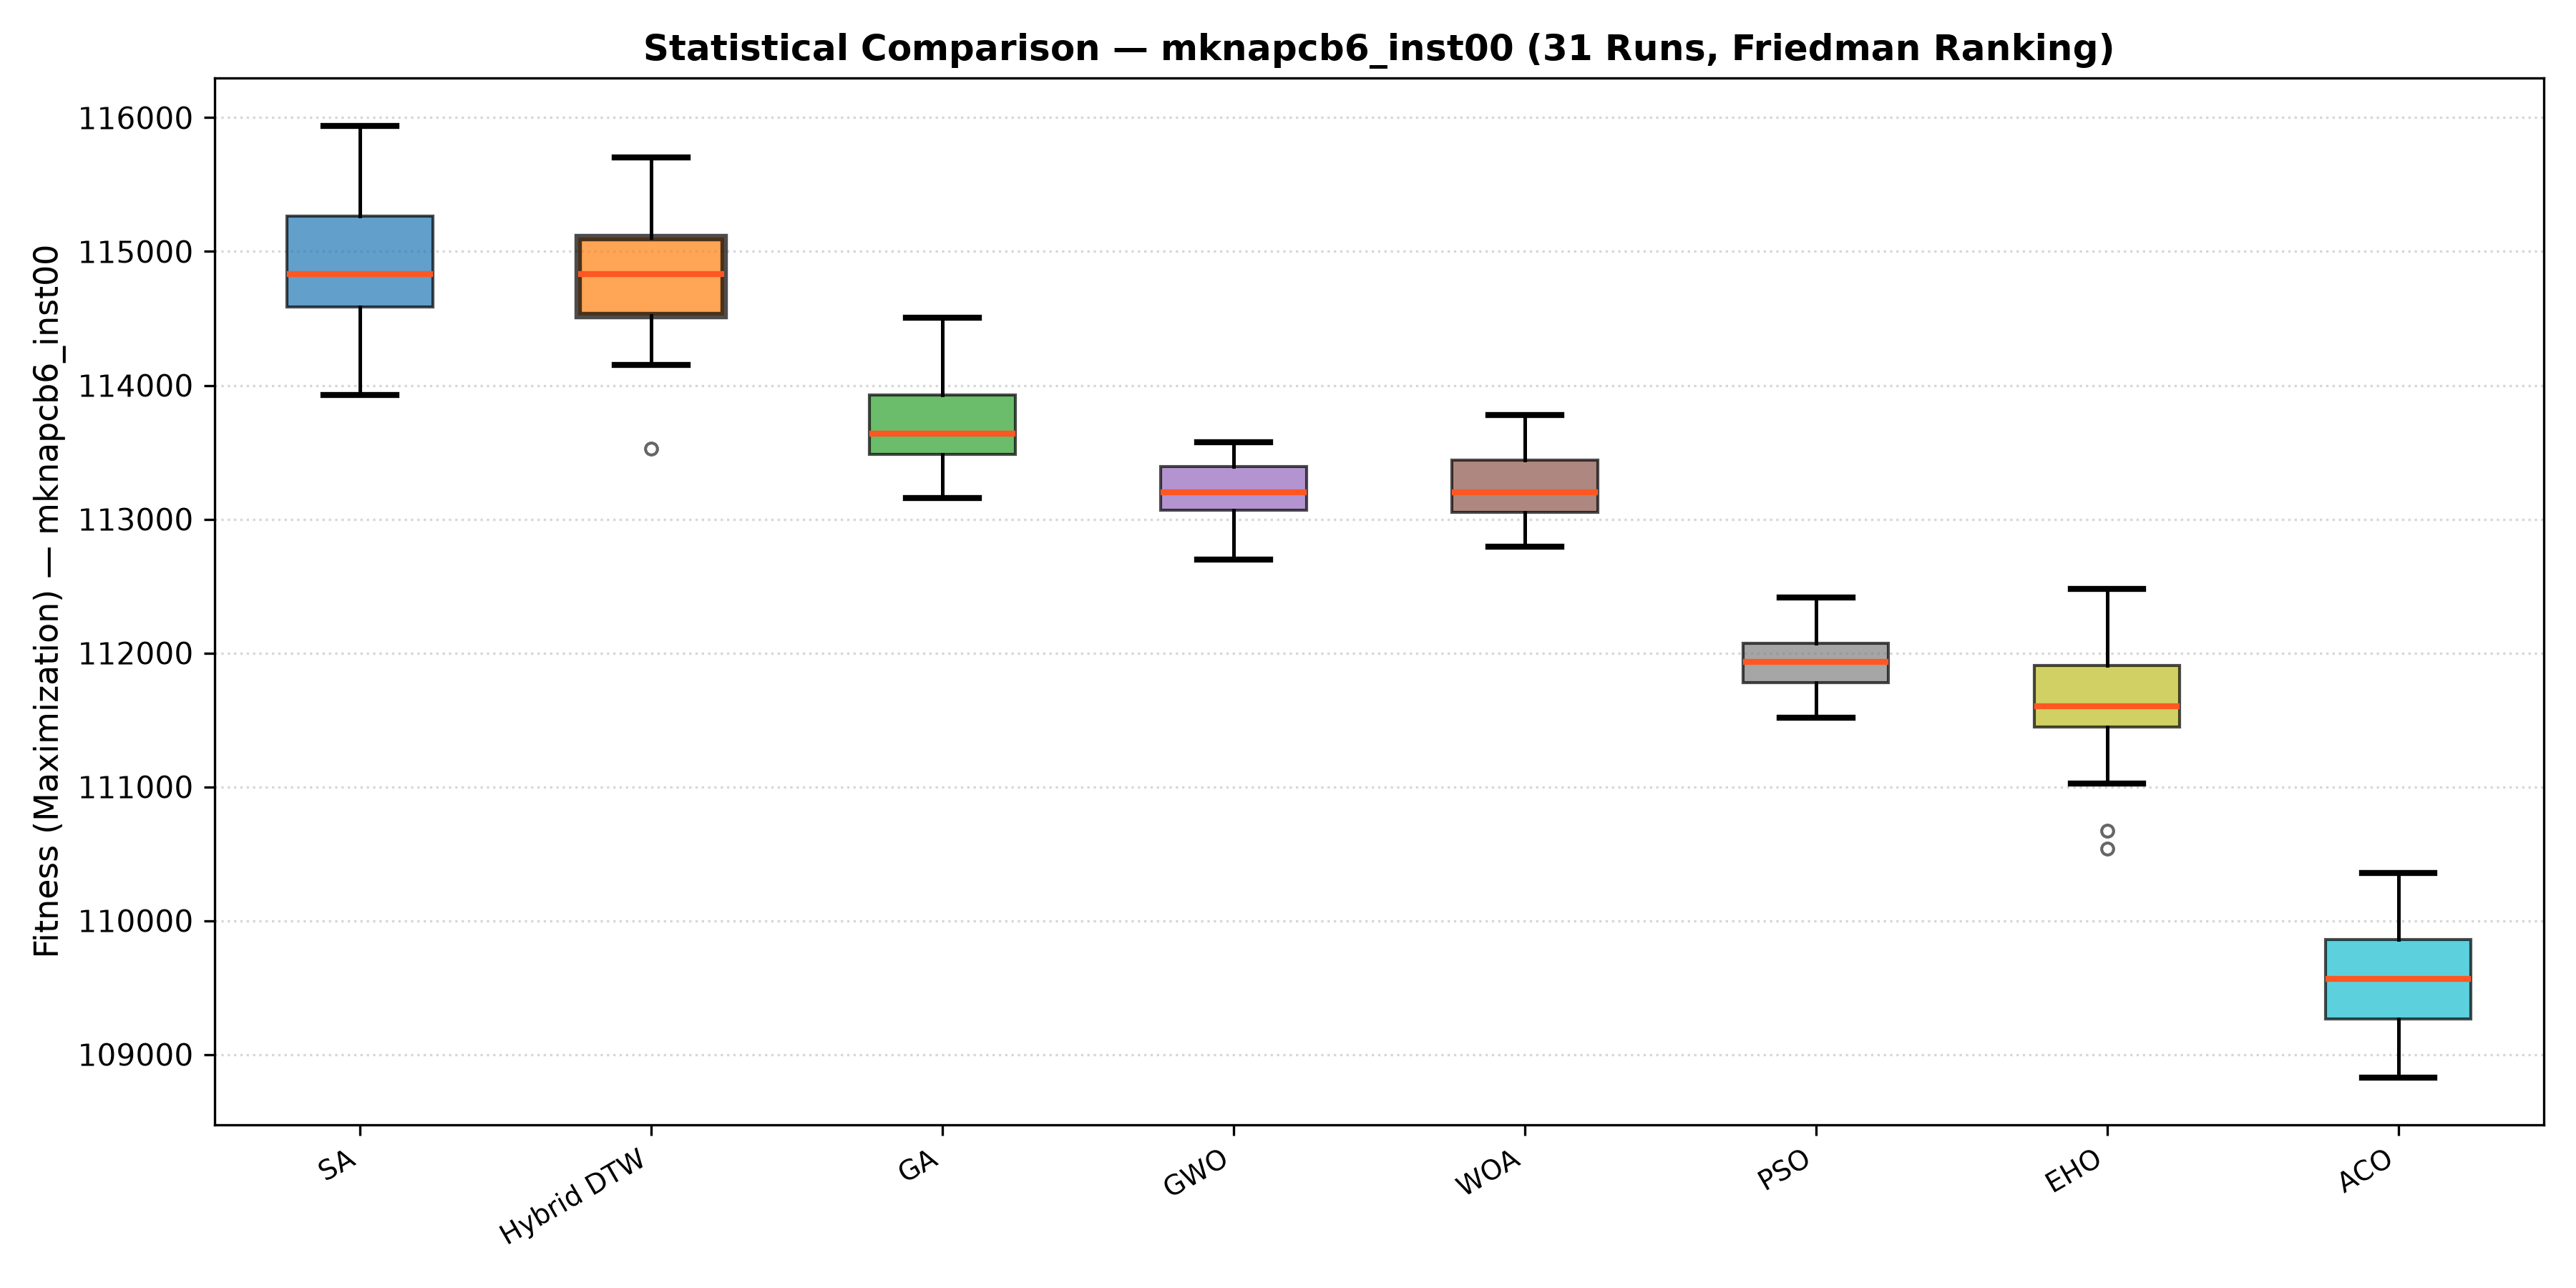
\includegraphics[width=0.32\textwidth]{imagenes_paper/mkp_dtw_3k_mknapcb6_comparativo_mh.png}}\hfill
\subfloat[Best-run convergence.]{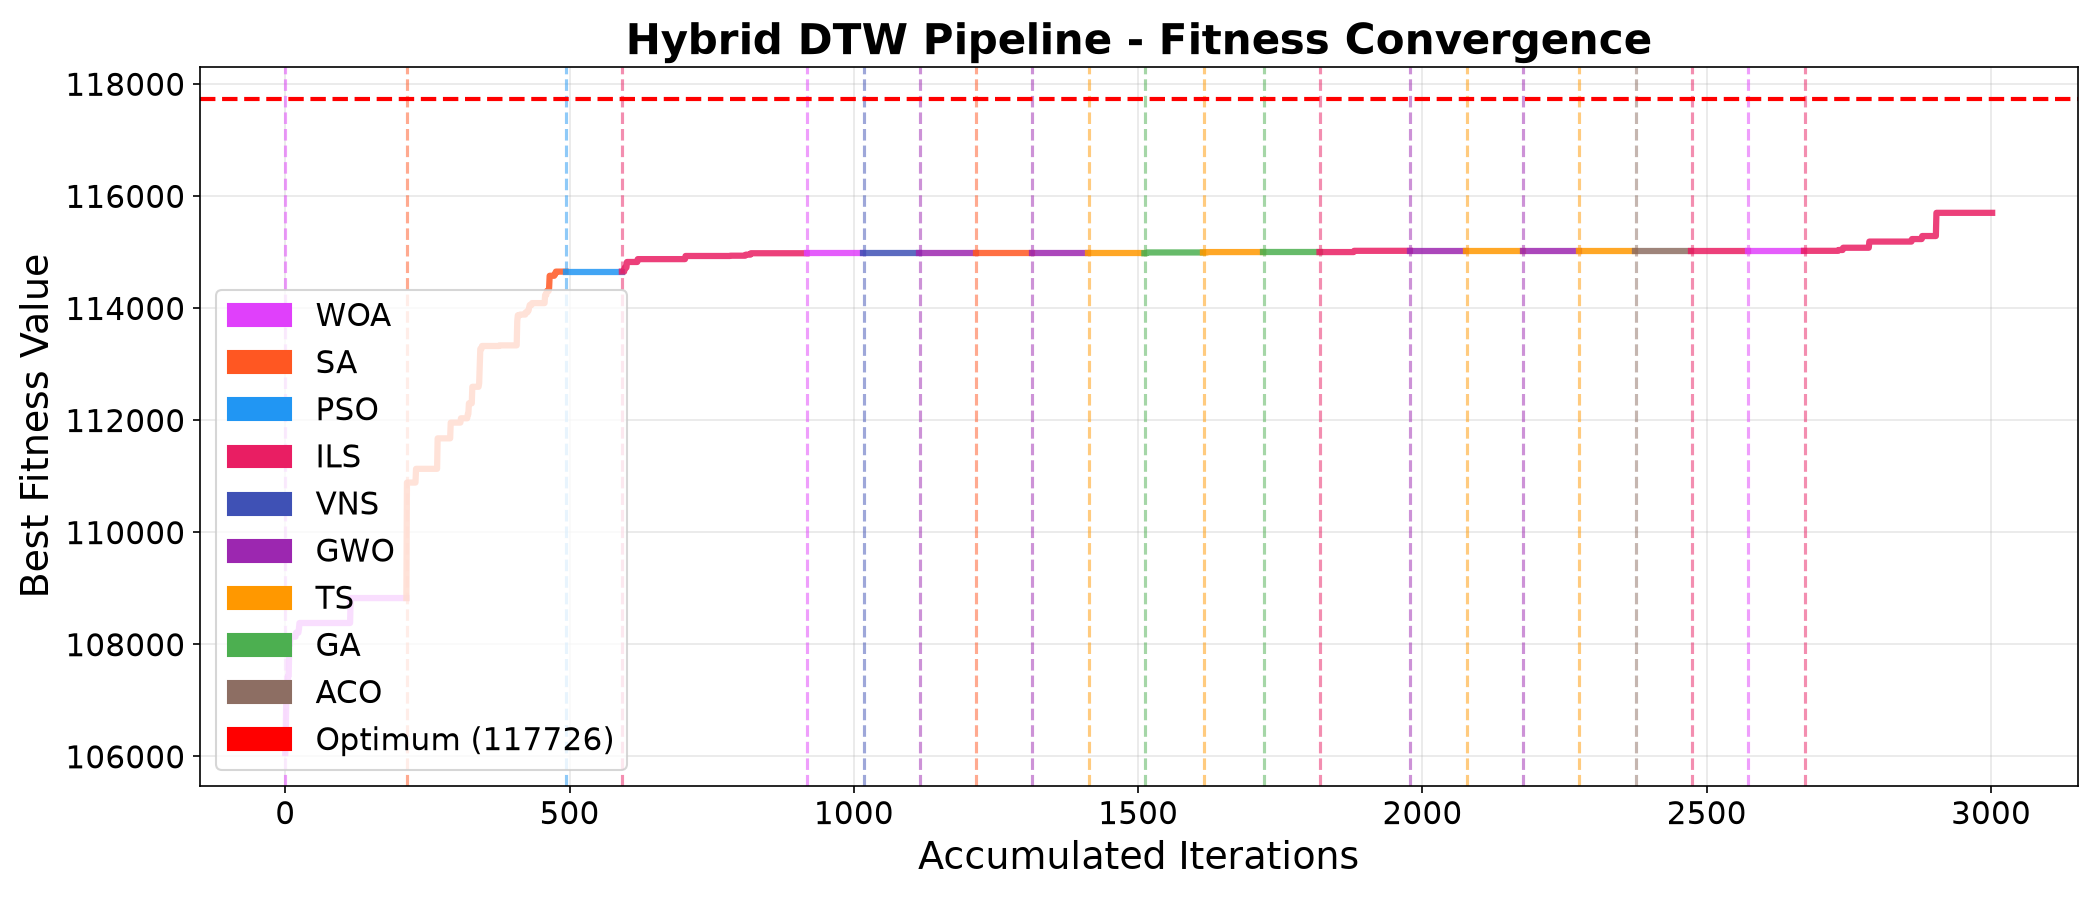
\includegraphics[width=0.32\textwidth]{imagenes_paper/mkp_dtw_3k_mknapcb6_convergencia.png}}\hfill
\subfloat[Elastic metric $\Delta=D_1-D_2$.]{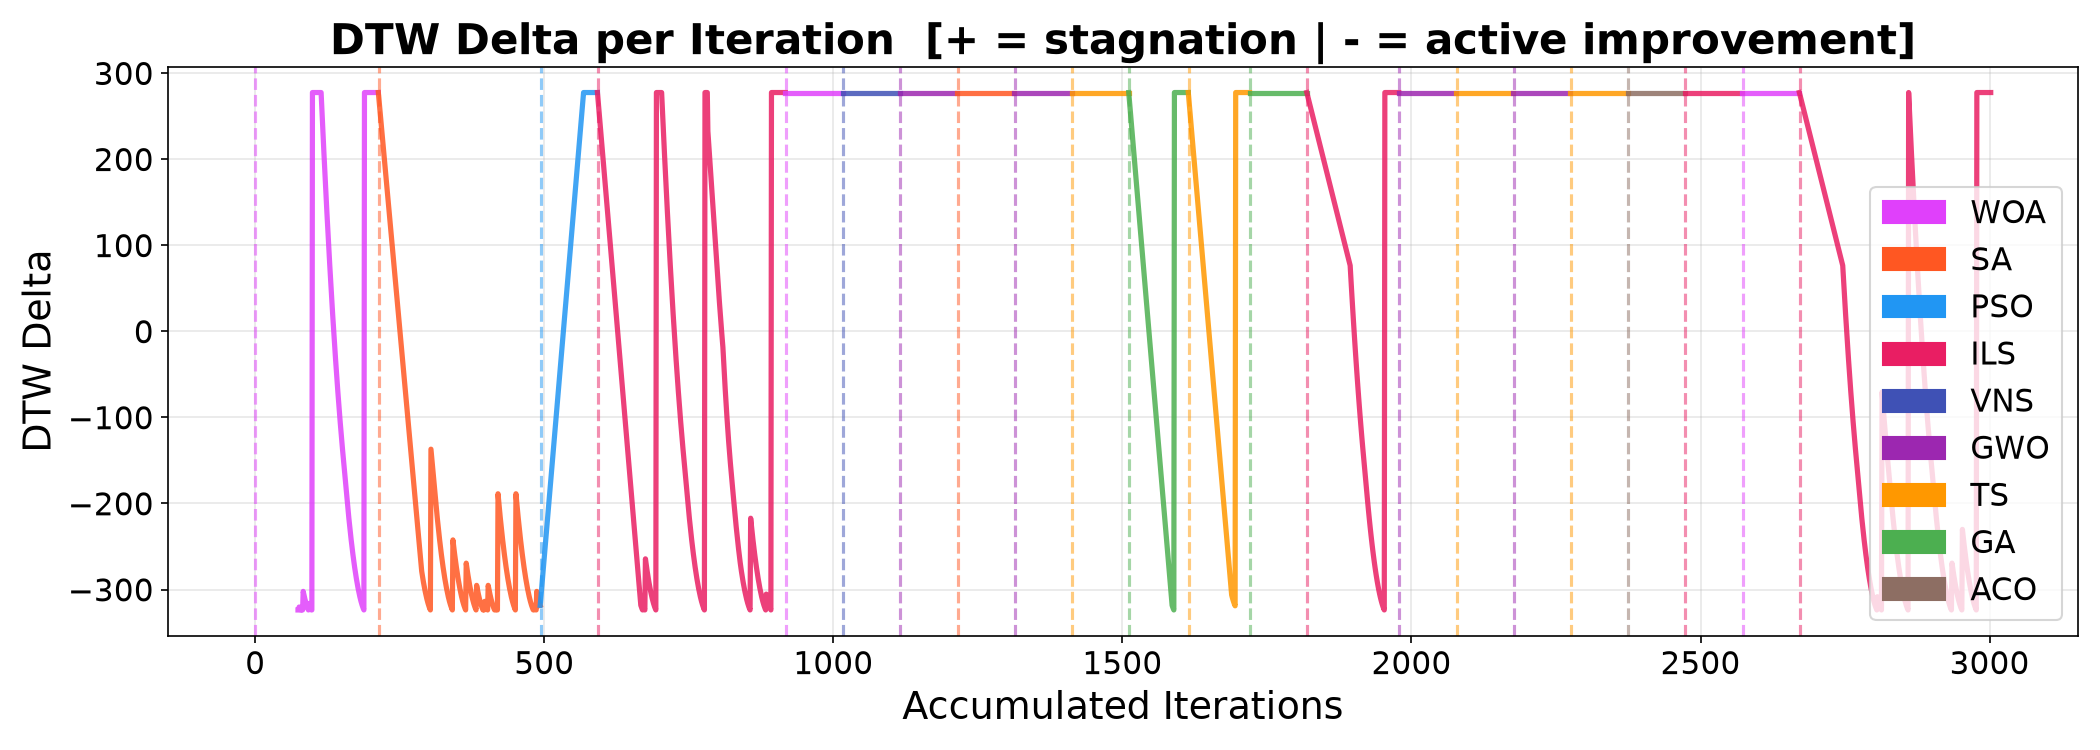
\includegraphics[width=0.32\textwidth]{imagenes_paper/mkp_dtw_3k_mknapcb6_delta.png}}
\caption{Diagnostic suite for instance \textbf{mknapcb6} ($n=500$, $m=10$) under the DTW framework with $T_{\max}=3{,}000$: (a)~final-fitness distribution over $N=31$ runs; (b)~convergence trajectory of the best run; (c)~elastic warping profile $\Delta$.}
\label{fig:mkp-best-cb6}
\end{figure}

% --- mknapcb7: DTW, 3,000 iterations ---
\begin{figure}[htbp]
\centering
\subfloat[Metaheuristic comparison.]{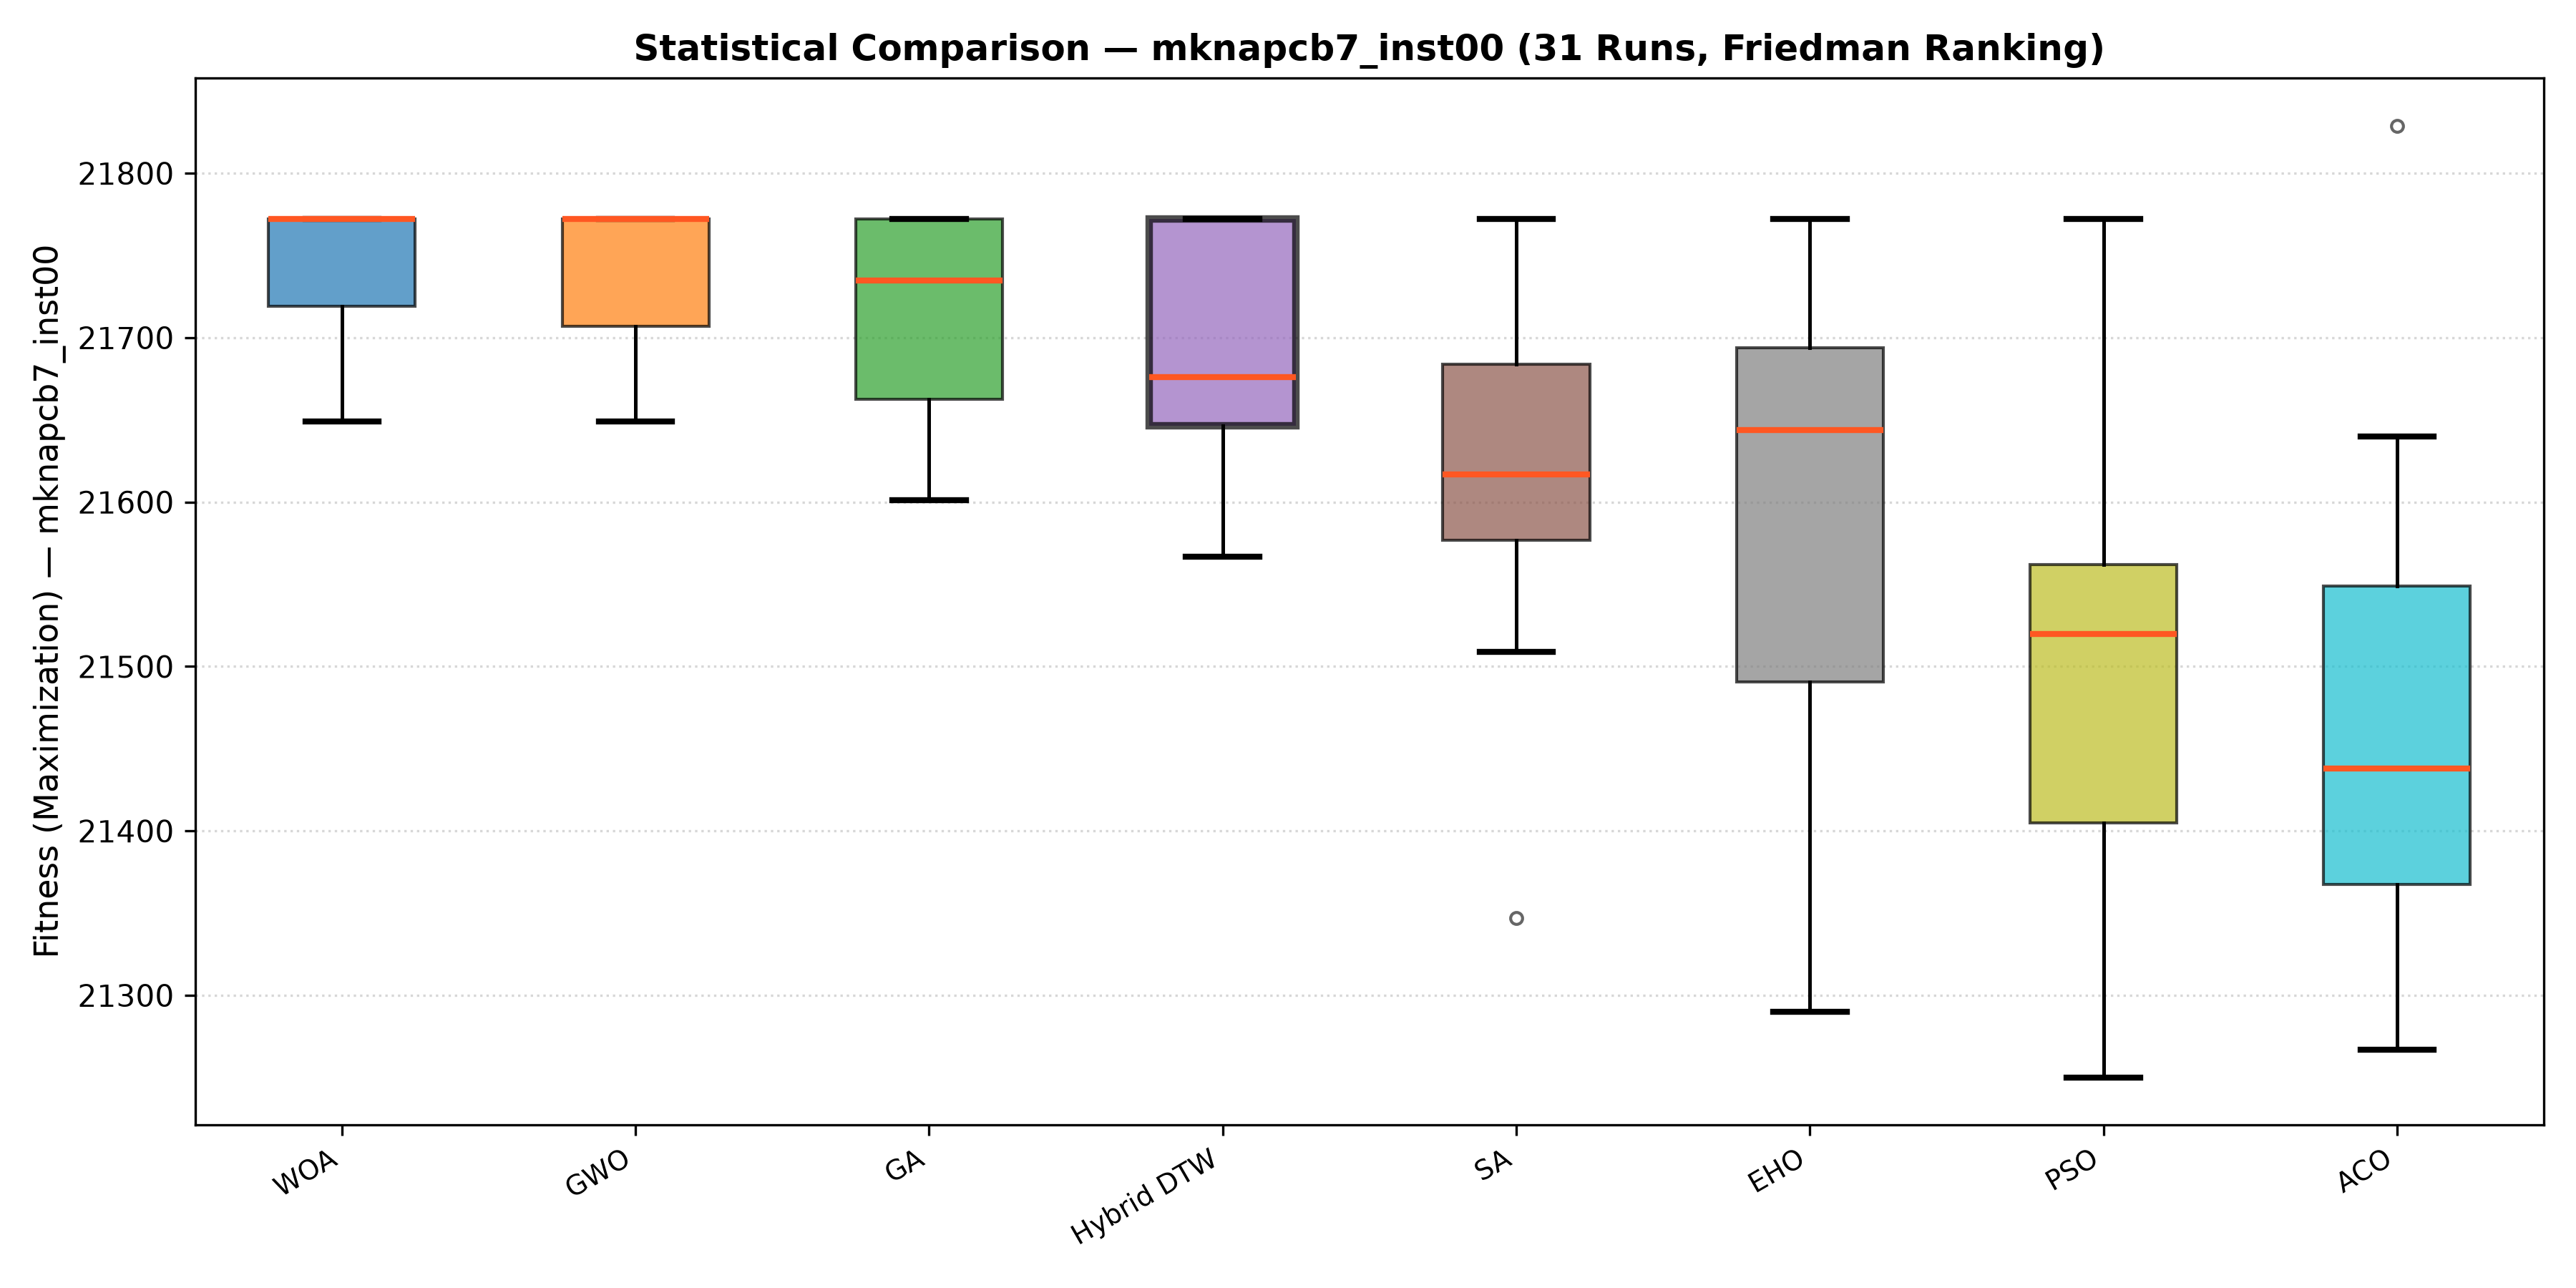
\includegraphics[width=0.32\textwidth]{imagenes_paper/mkp_dtw_3k_mknapcb7_comparativo_mh.png}}\hfill
\subfloat[Best-run convergence.]{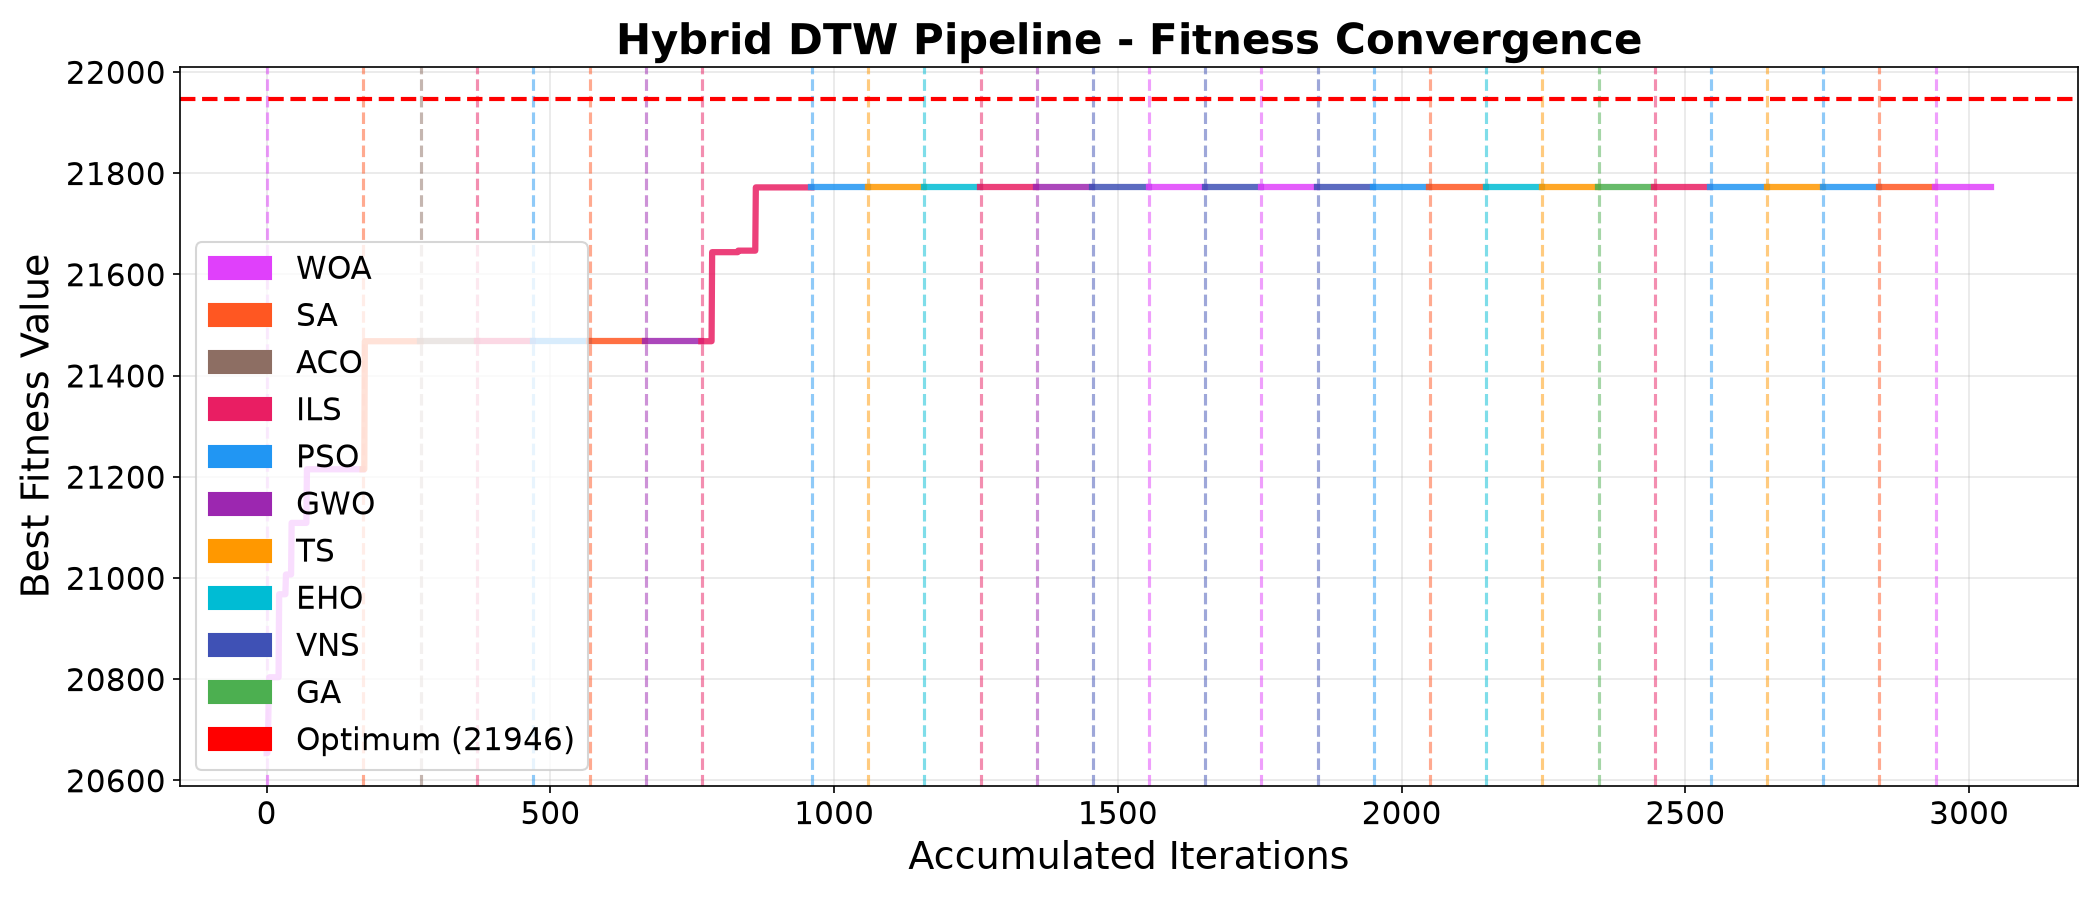
\includegraphics[width=0.32\textwidth]{imagenes_paper/mkp_dtw_3k_mknapcb7_convergencia.png}}\hfill
\subfloat[Elastic metric $\Delta=D_1-D_2$.]{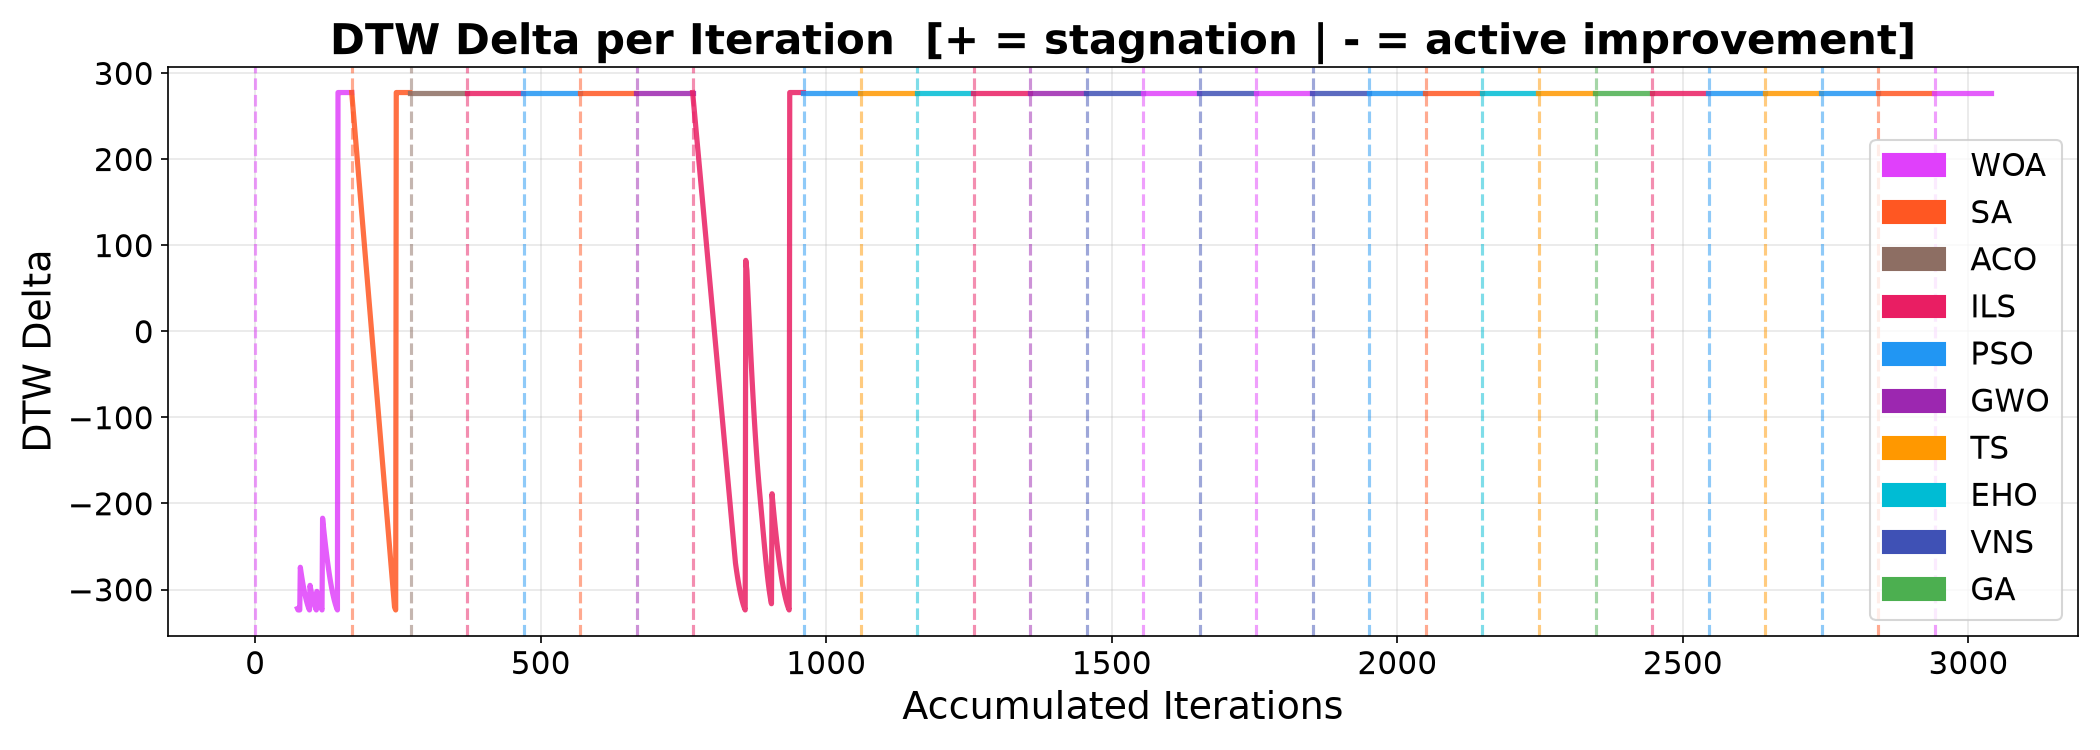
\includegraphics[width=0.32\textwidth]{imagenes_paper/mkp_dtw_3k_mknapcb7_delta.png}}
\caption{Diagnostic suite for instance \textbf{mknapcb7} ($n=100$, $m=30$) under the DTW framework with $T_{\max}=3{,}000$: (a)~final-fitness distribution over $N=31$ runs; (b)~convergence trajectory of the best run; (c)~elastic warping profile $\Delta$.}
\label{fig:mkp-best-cb7}
\end{figure}

% --- mknapcb8: DTW, 3,000 iterations ---
\begin{figure}[htbp]
\centering
\subfloat[Metaheuristic comparison.]{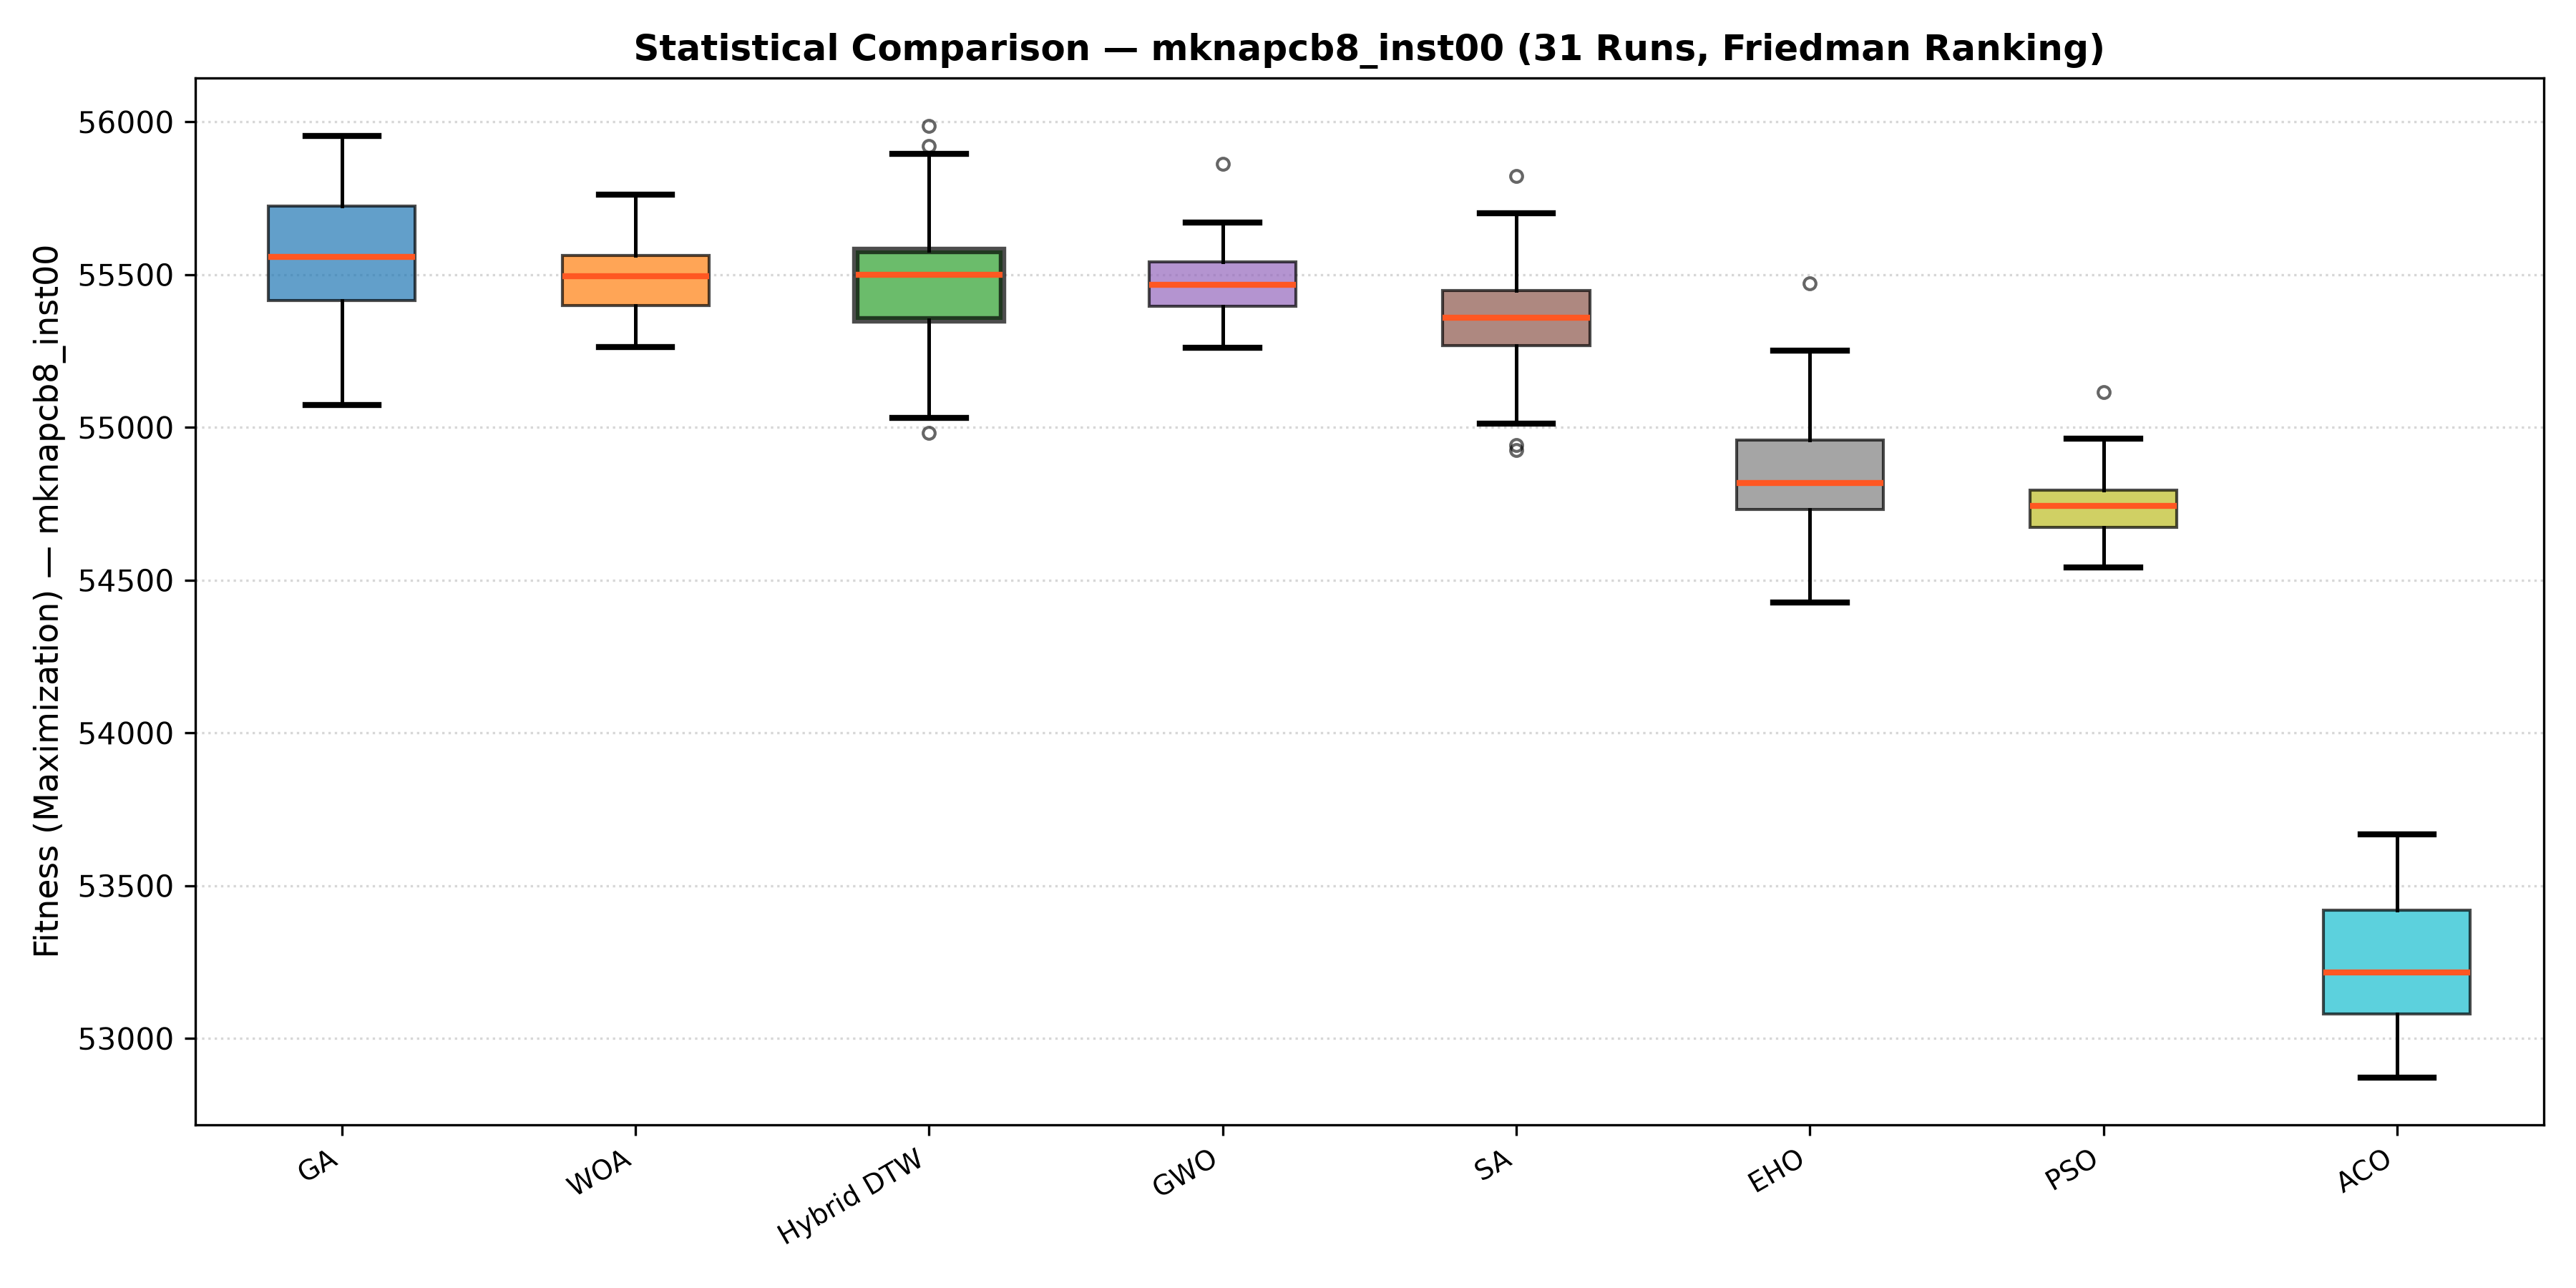
\includegraphics[width=0.32\textwidth]{imagenes_paper/mkp_dtw_3k_mknapcb8_comparativo_mh.png}}\hfill
\subfloat[Best-run convergence.]{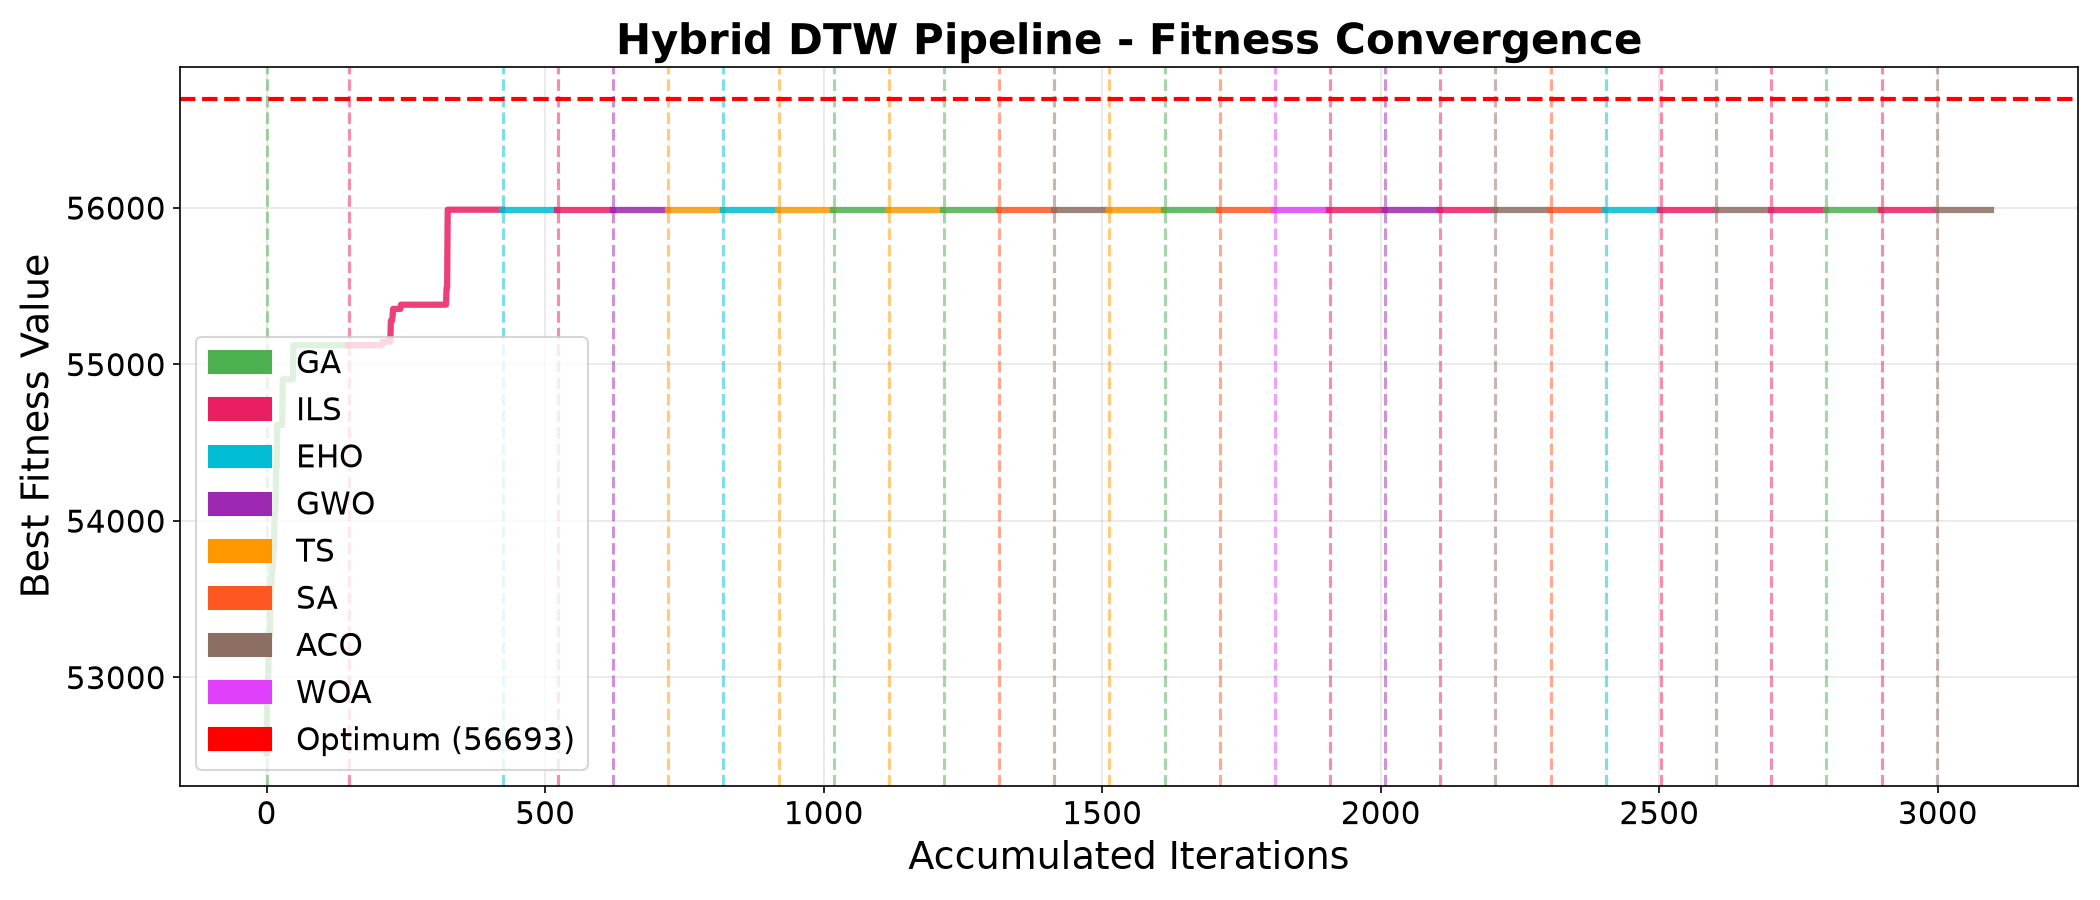
\includegraphics[width=0.32\textwidth]{imagenes_paper/mkp_dtw_3k_mknapcb8_convergencia.png}}\hfill
\subfloat[Elastic metric $\Delta=D_1-D_2$.]{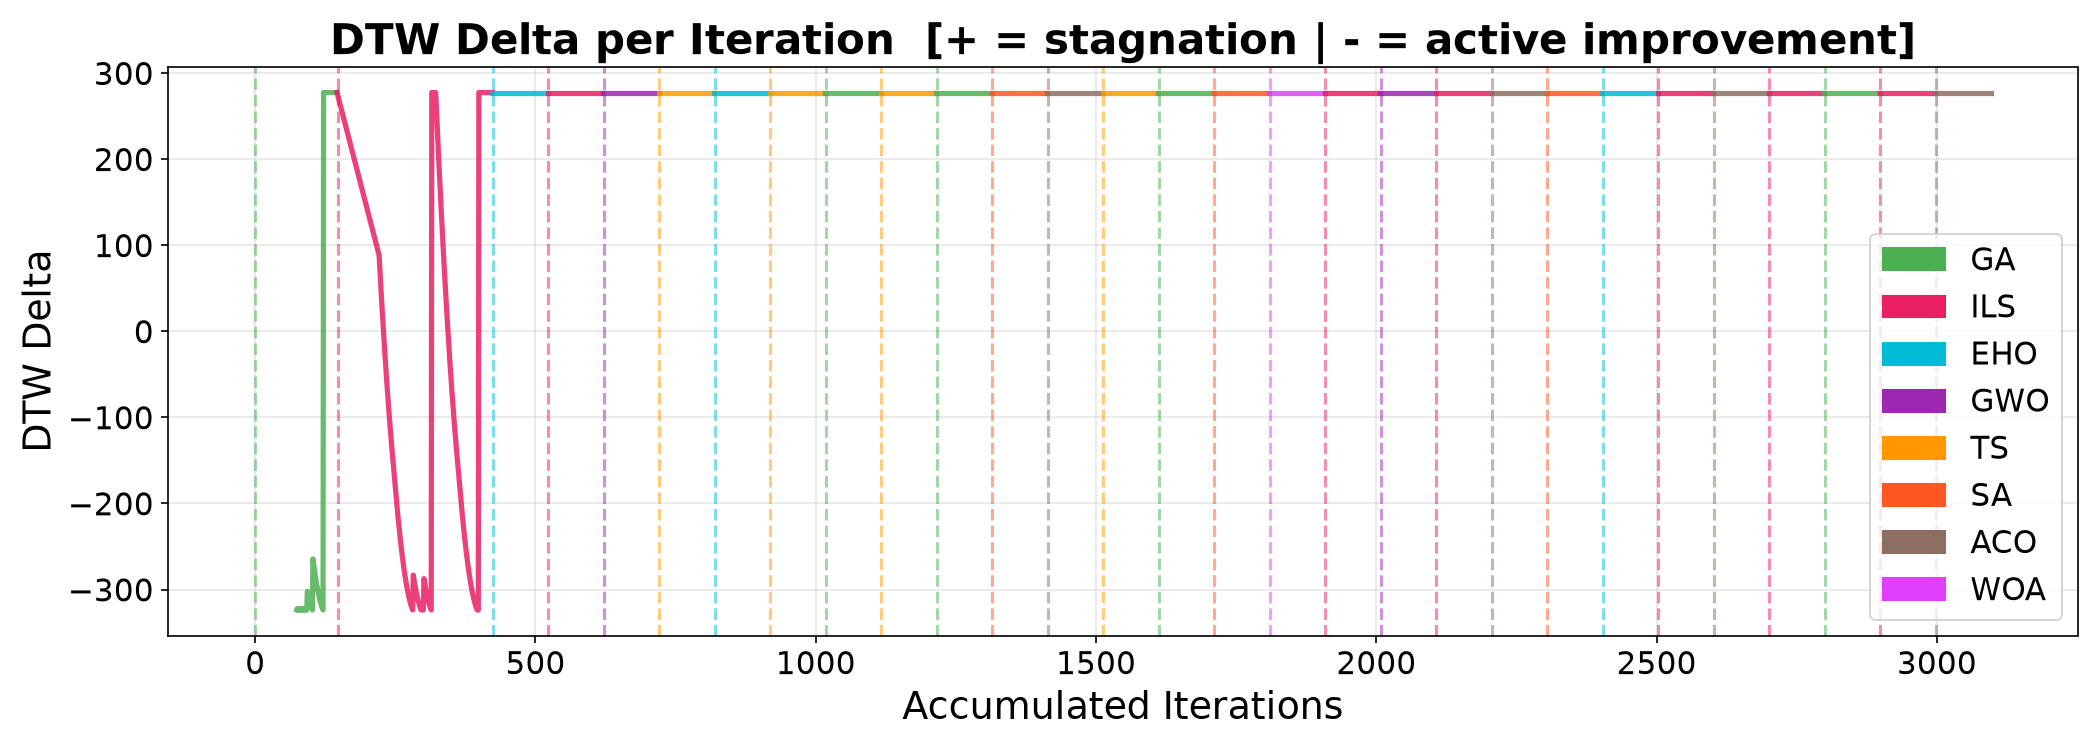
\includegraphics[width=0.32\textwidth]{imagenes_paper/mkp_dtw_3k_mknapcb8_delta.png}}
\caption{Diagnostic suite for instance \textbf{mknapcb8} ($n=250$, $m=30$) under the DTW framework with $T_{\max}=3{,}000$: (a)~final-fitness distribution over $N=31$ runs; (b)~convergence trajectory of the best run; (c)~elastic warping profile $\Delta$.}
\label{fig:mkp-best-cb8}
\end{figure}

% --- mknapcb9: DDTW, 3,000 iterations ---
\begin{figure}[htbp]
\centering
\subfloat[Metaheuristic comparison.]{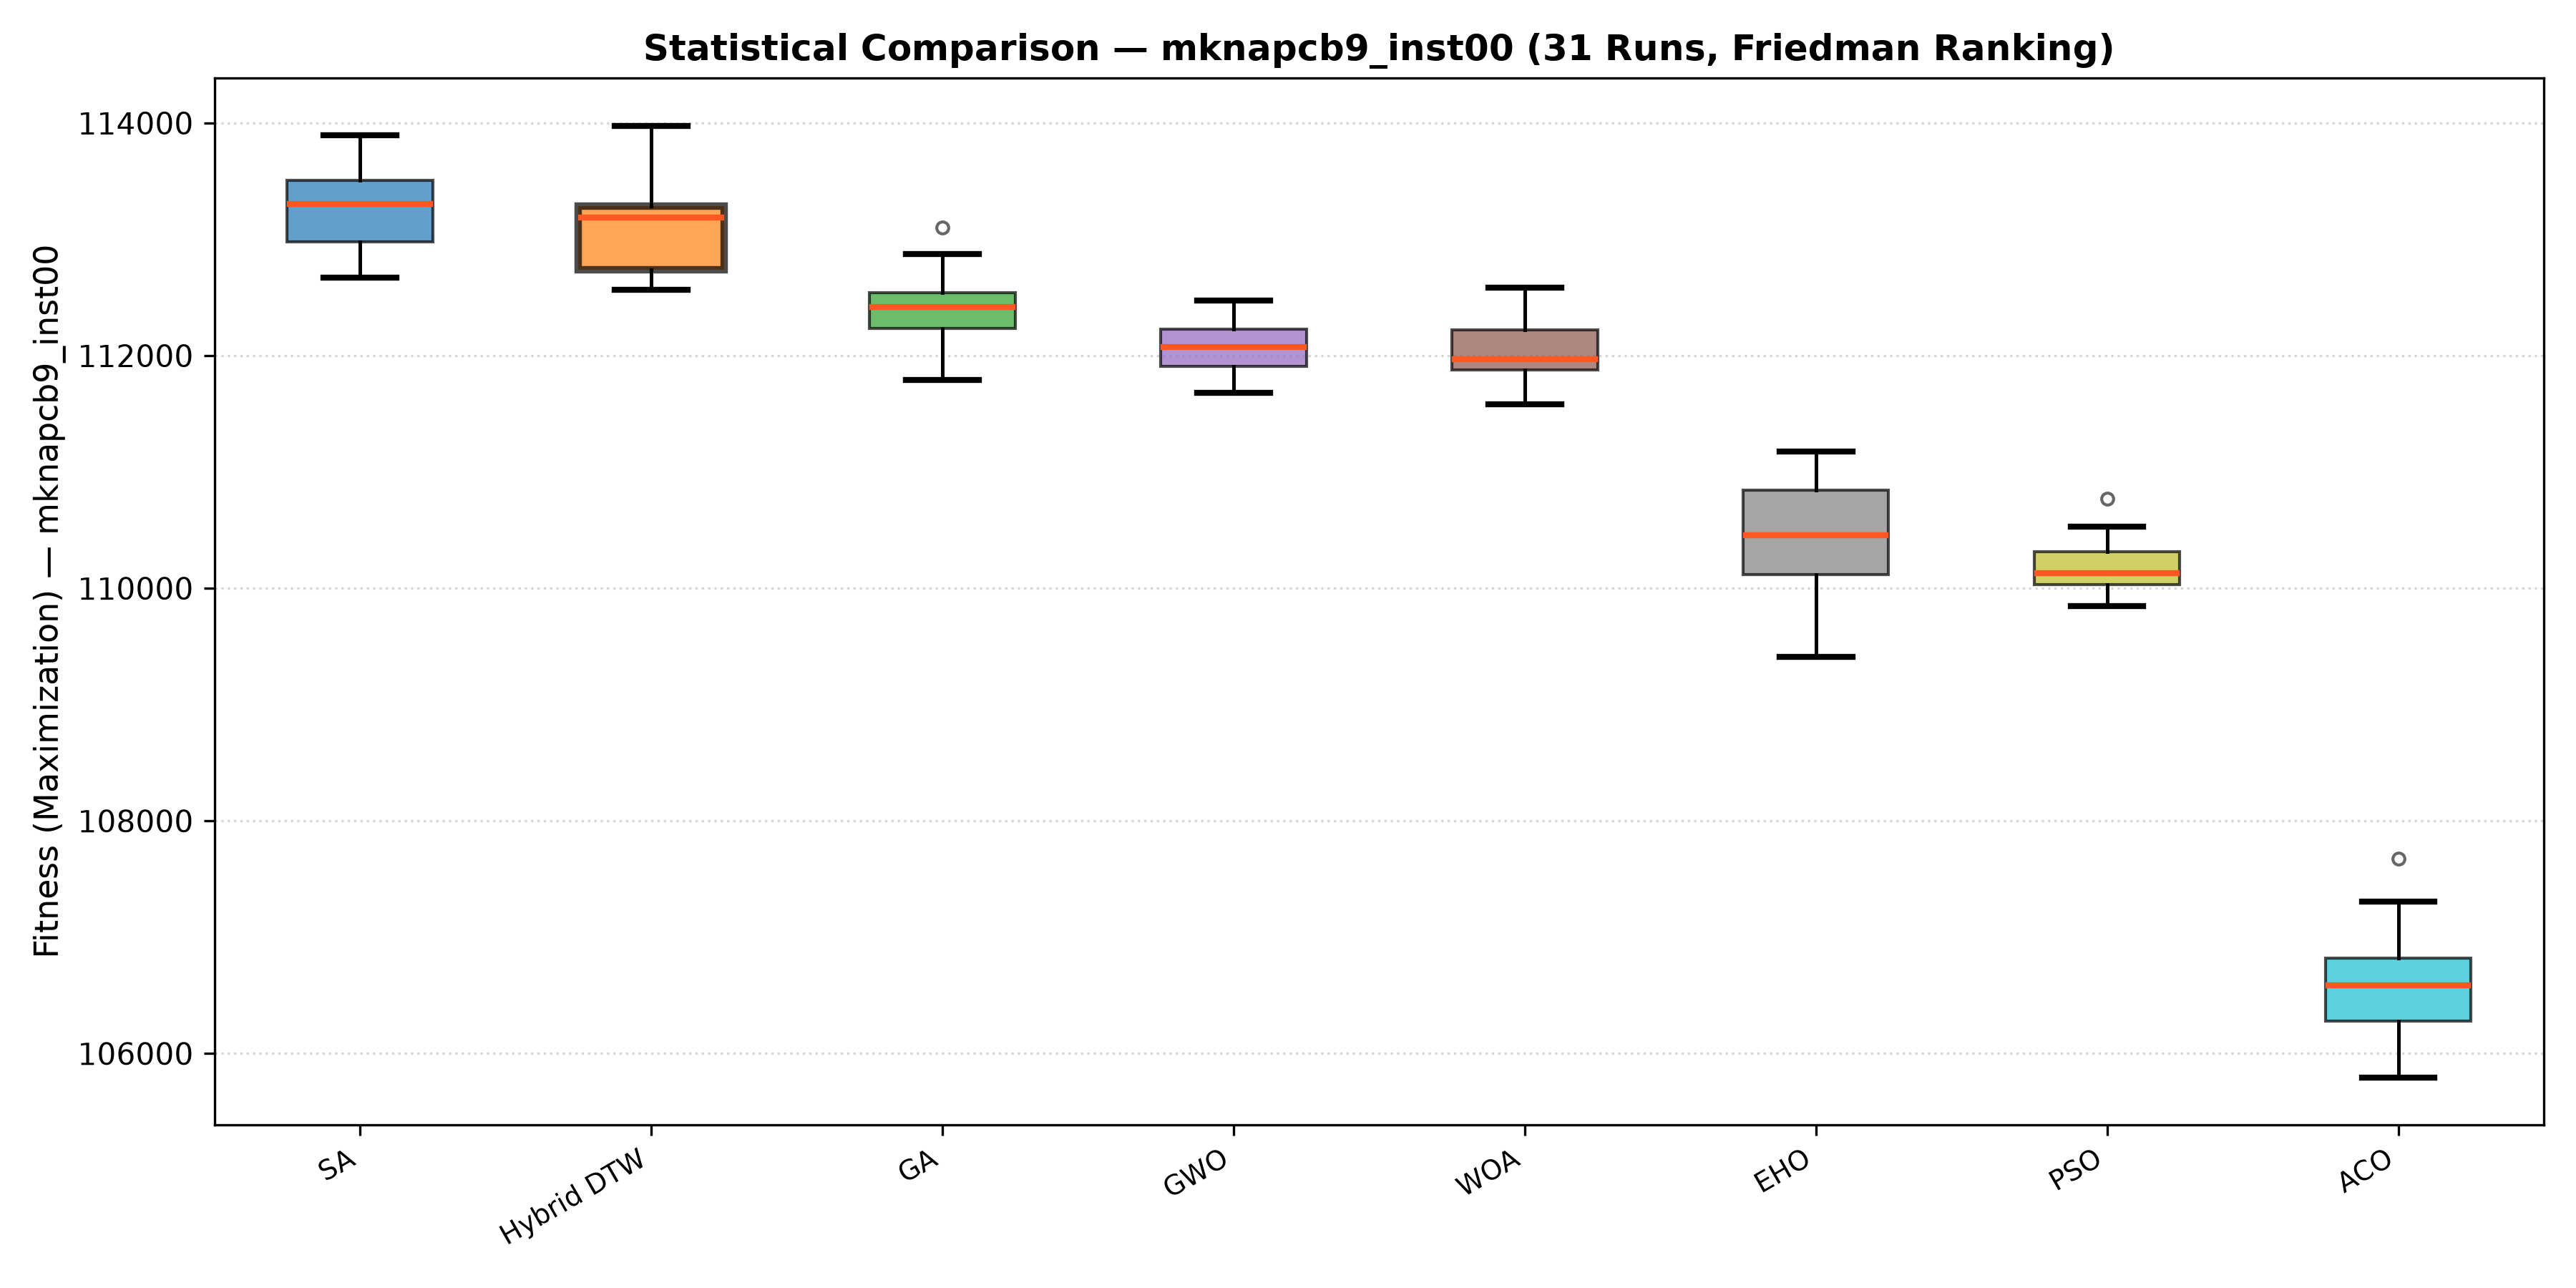
\includegraphics[width=0.32\textwidth]{imagenes_paper/mkp_ddtw_3k_mknapcb9_comparativo_mh.png}}\hfill
\subfloat[Best-run convergence.]{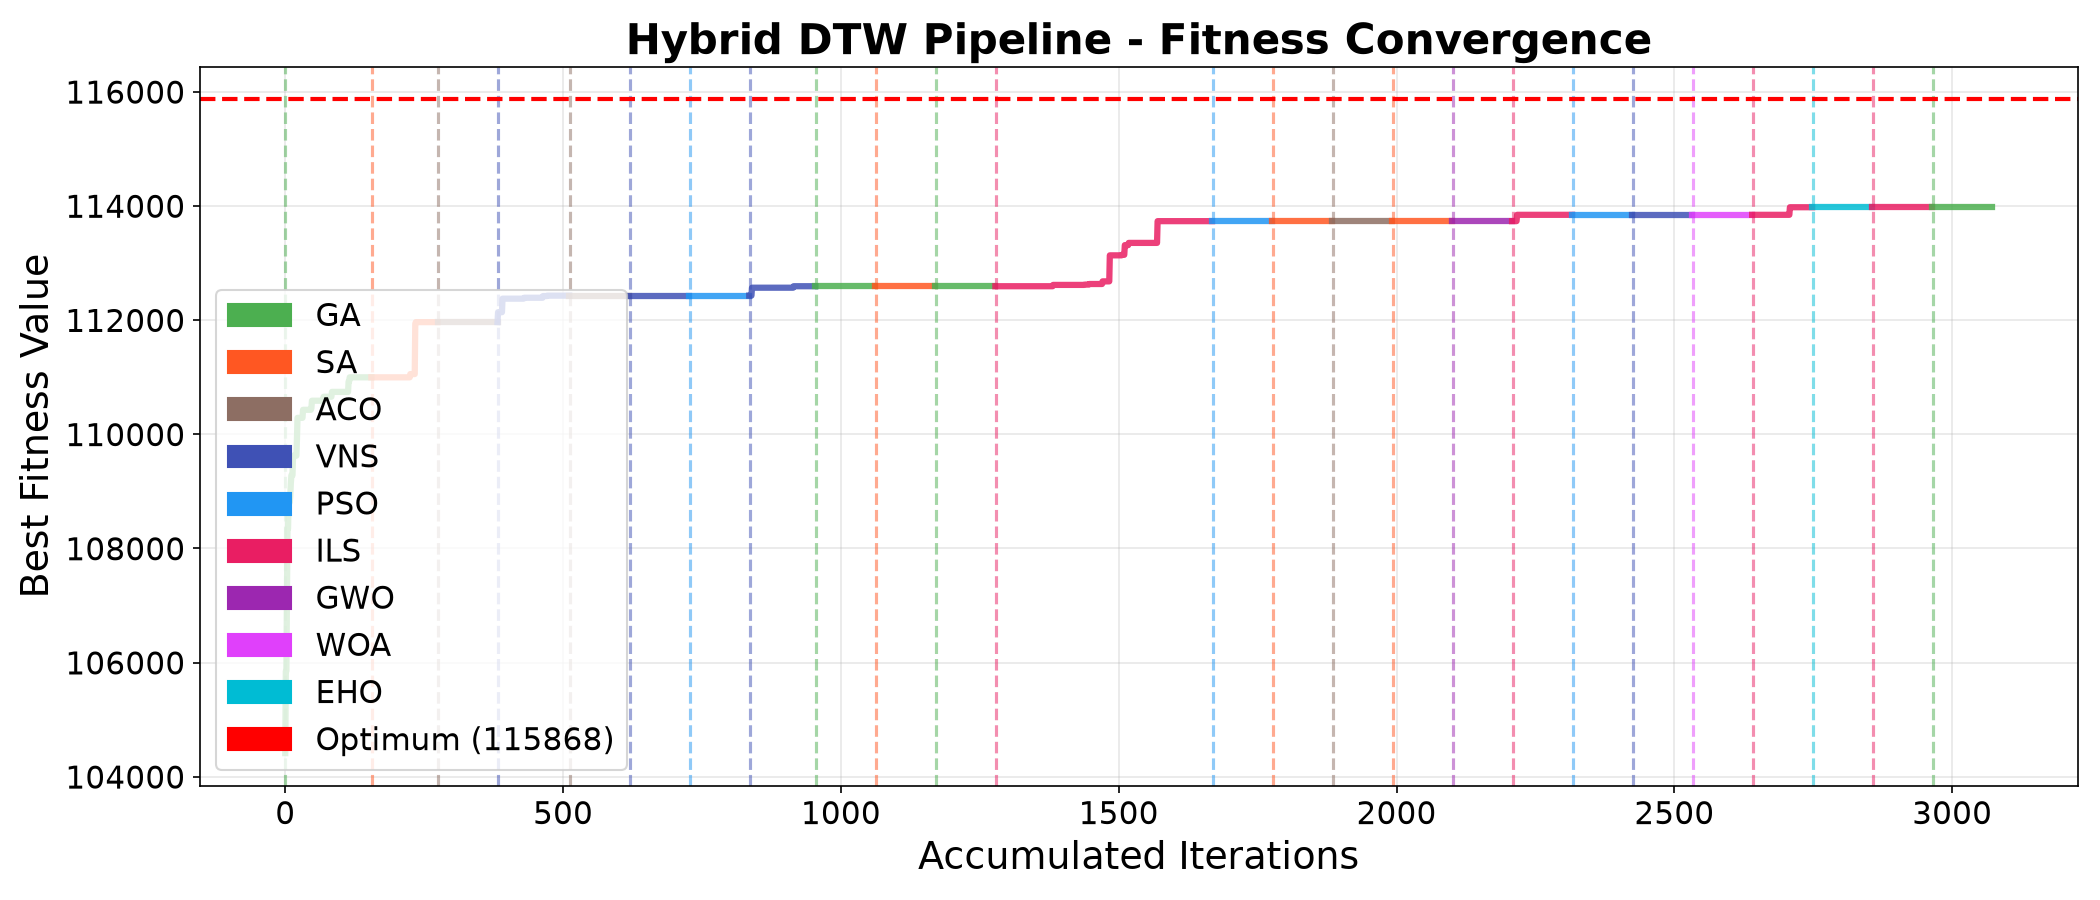
\includegraphics[width=0.32\textwidth]{imagenes_paper/mkp_ddtw_3k_mknapcb9_convergencia.png}}\hfill
\subfloat[Elastic metric $\Delta=D_1-D_2$.]{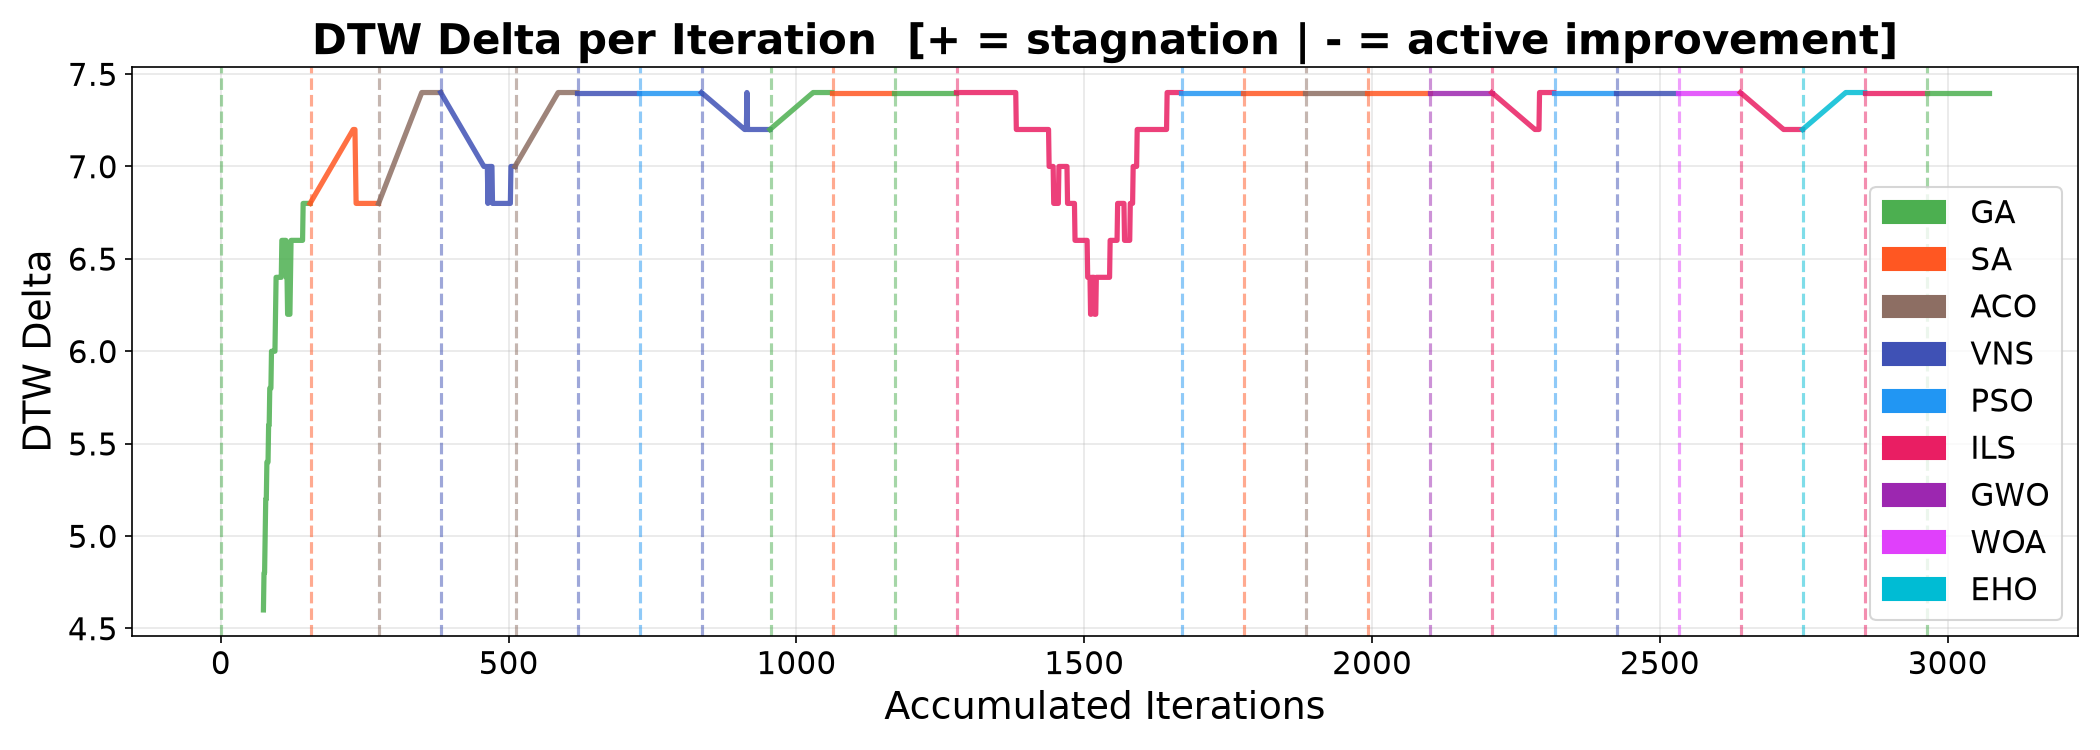
\includegraphics[width=0.32\textwidth]{imagenes_paper/mkp_ddtw_3k_mknapcb9_delta.png}}
\caption{Diagnostic suite for instance \textbf{mknapcb9} ($n=500$, $m=30$) under the DDTW framework with $T_{\max}=3{,}000$: (a)~final-fitness distribution over $N=31$ runs; (b)~convergence trajectory of the best run; (c)~elastic warping profile $\Delta$.}
\label{fig:mkp-best-cb9}
\end{figure}

% Required packages: graphicx, subfig (or subcaption with \subfloat redefined).

% Each figure shows the best-performing framework configuration for the
% corresponding instance, selected by highest mean fitness over 31 runs.
% DTW--3K is best for mknapcb1 and mknapcb3--mknapcb8;
% DDTW--3K is best for mknapcb2 and mknapcb9.

Figures~\ref{fig:mkp-best-cb1}--\ref{fig:mkp-best-cb9} present the
diagnostic suite for each of the nine Chu--Beasley MKP instances under its
best-performing framework configuration, selected by highest mean fitness
over the 31 runs, with corresponding executions treated as paired. DTW with $T_{\max}=3{,}000$ achieved the
highest mean in seven instances (mknapcb1 and mknapcb3--mknapcb8), while
DDTW with $T_{\max}=3{,}000$ was superior for mknapcb2 and mknapcb9.
Each figure comprises three panels: (a)~a box-plot comparing the
final-fitness distributions of the hybrid framework against the standalone
metaheuristics over the 31 runs, allowing visual assessment of both central
tendency and dispersion; (b)~the convergence trajectory of the best run,
showing the evolution of the incumbent fitness along with the solver
transitions triggered by the stagnation monitor; and (c)~the elastic
warping profile $\Delta = D_1 - D_2$, where positive values indicate
detected stagnation phases and negative values correspond to periods of
active improvement.

% --- mknapcb1: DTW, 3,000 iterations ---
\begin{figure}[htbp]
\centering
\subfloat[Metaheuristic comparison.]{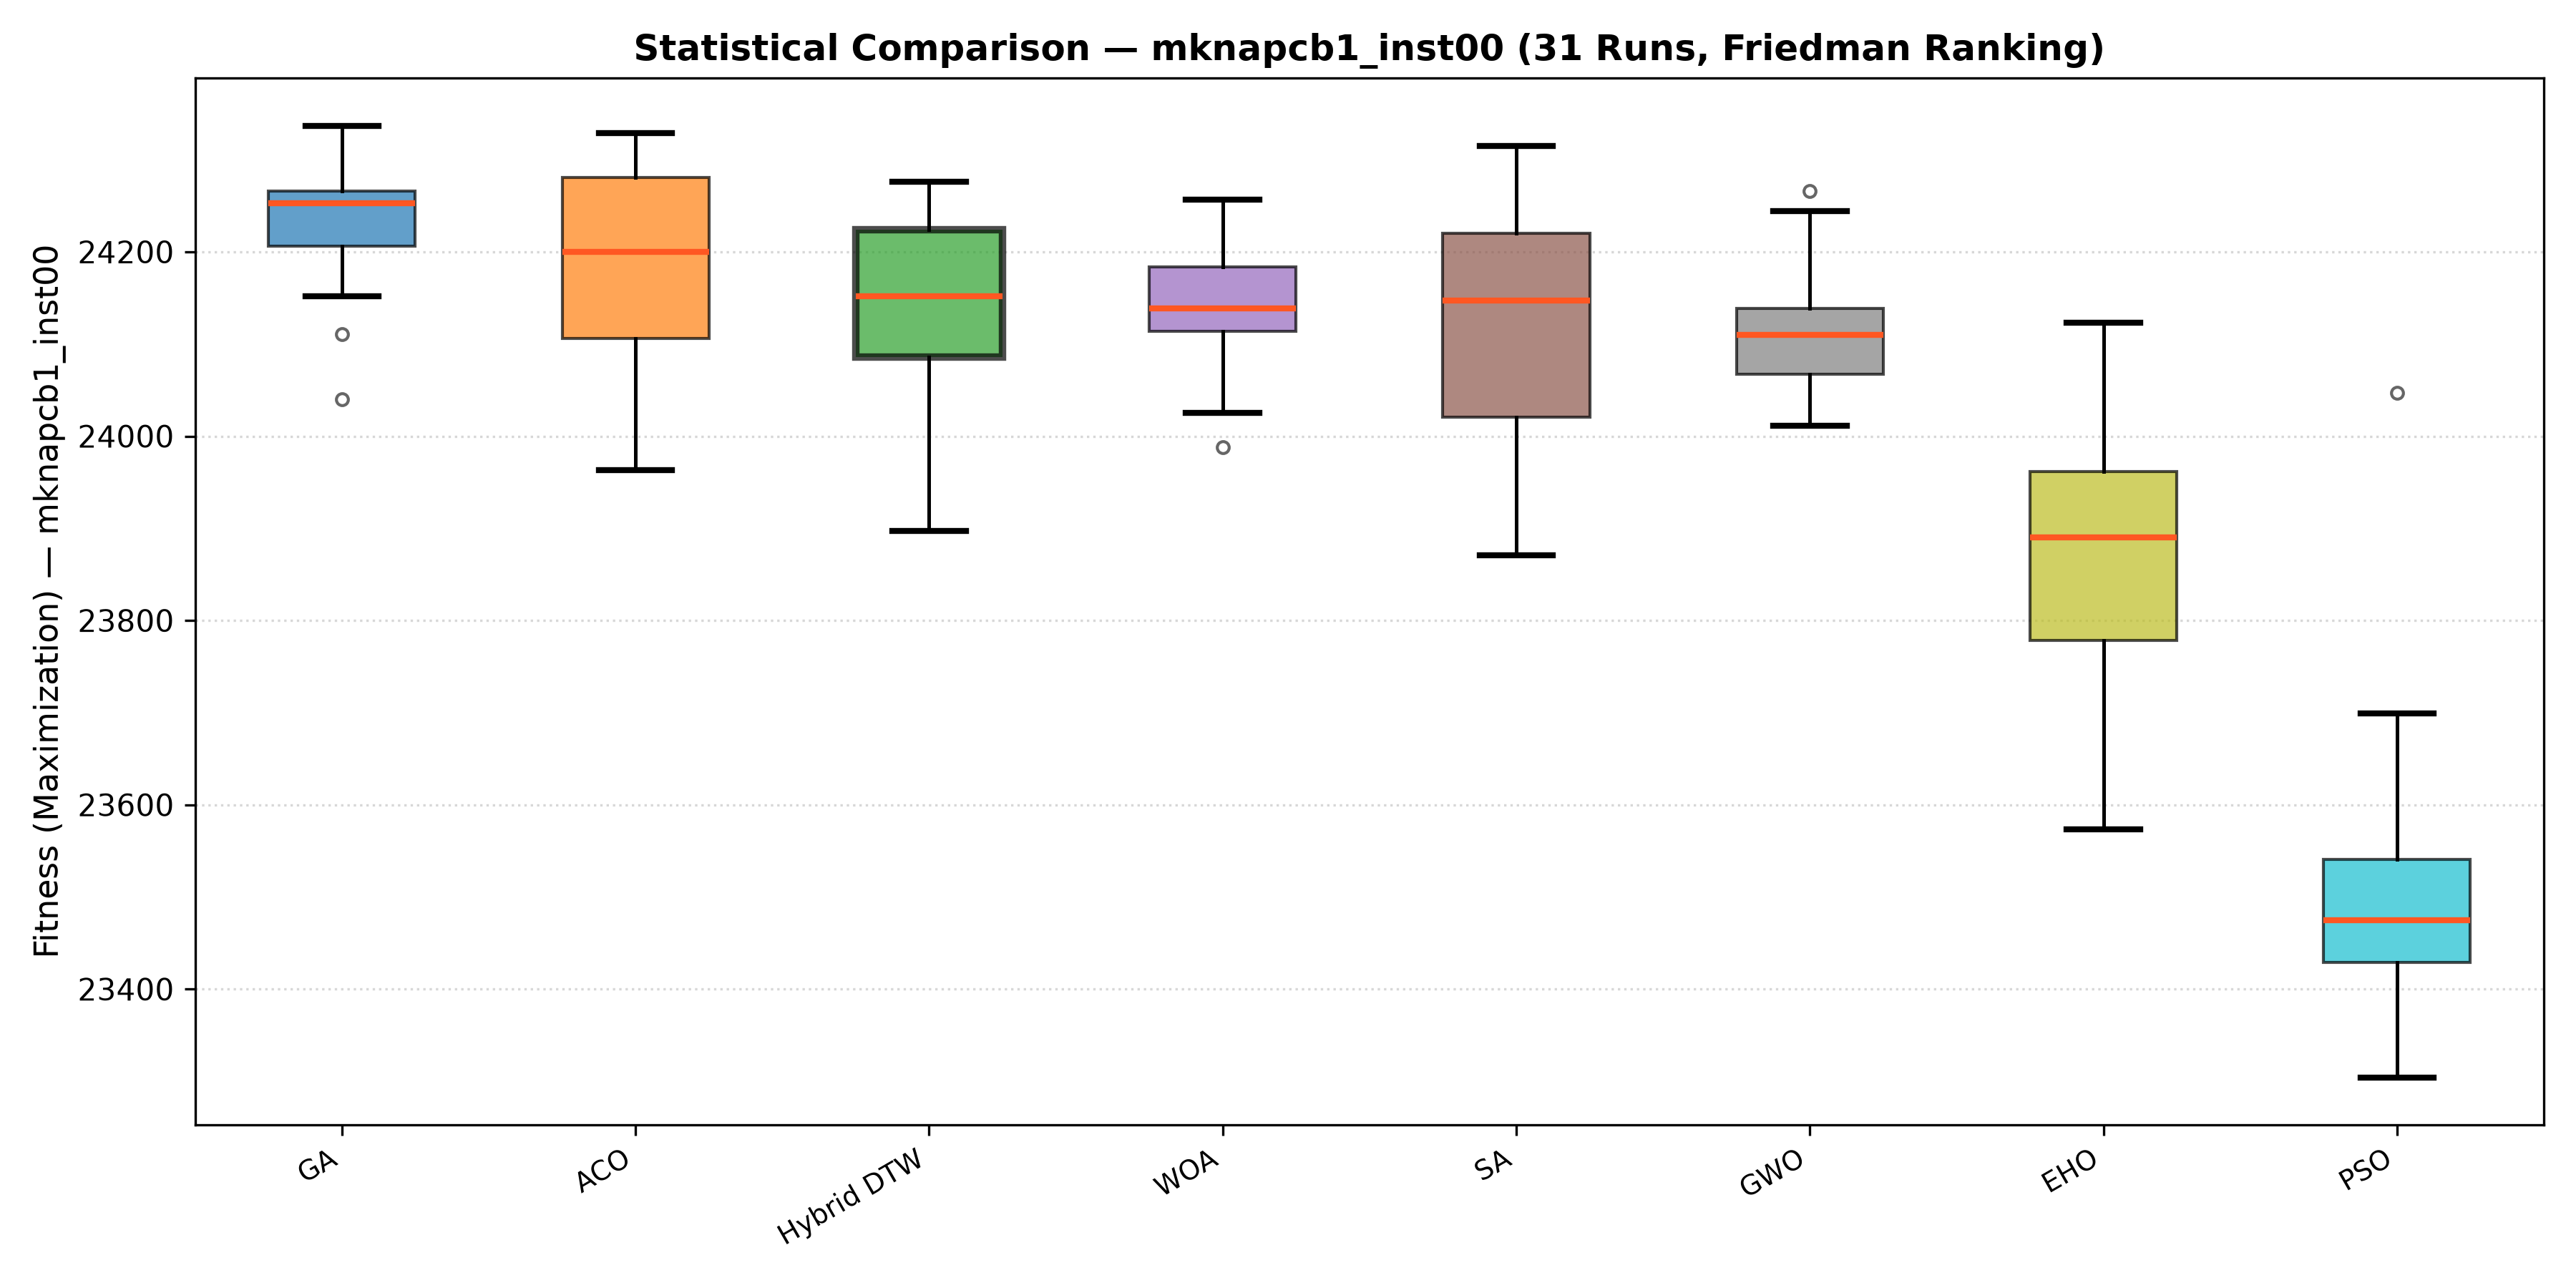
\includegraphics[width=0.32\textwidth]{imagenes_paper/mkp_dtw_3k_mknapcb1_comparativo_mh.png}}\hfill
\subfloat[Best-run convergence.]{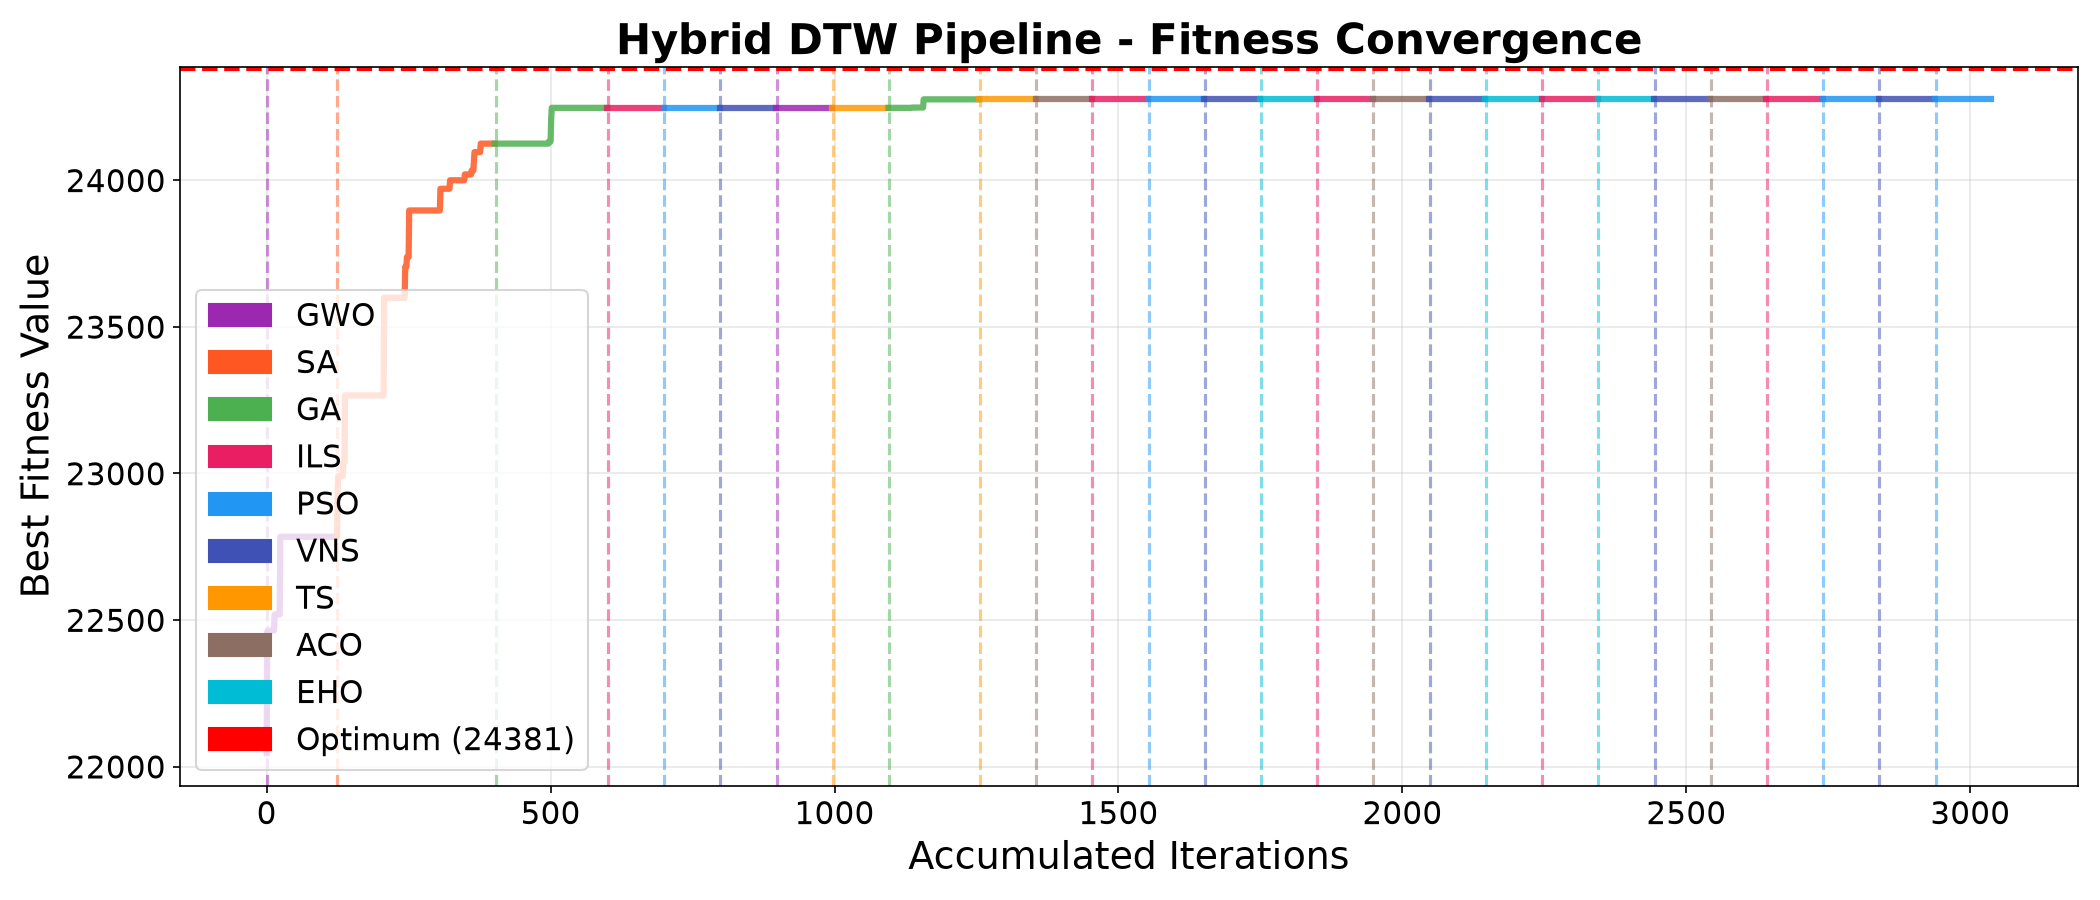
\includegraphics[width=0.32\textwidth]{imagenes_paper/mkp_dtw_3k_mknapcb1_convergencia.png}}\hfill
\subfloat[Elastic metric $\Delta=D_1-D_2$.]{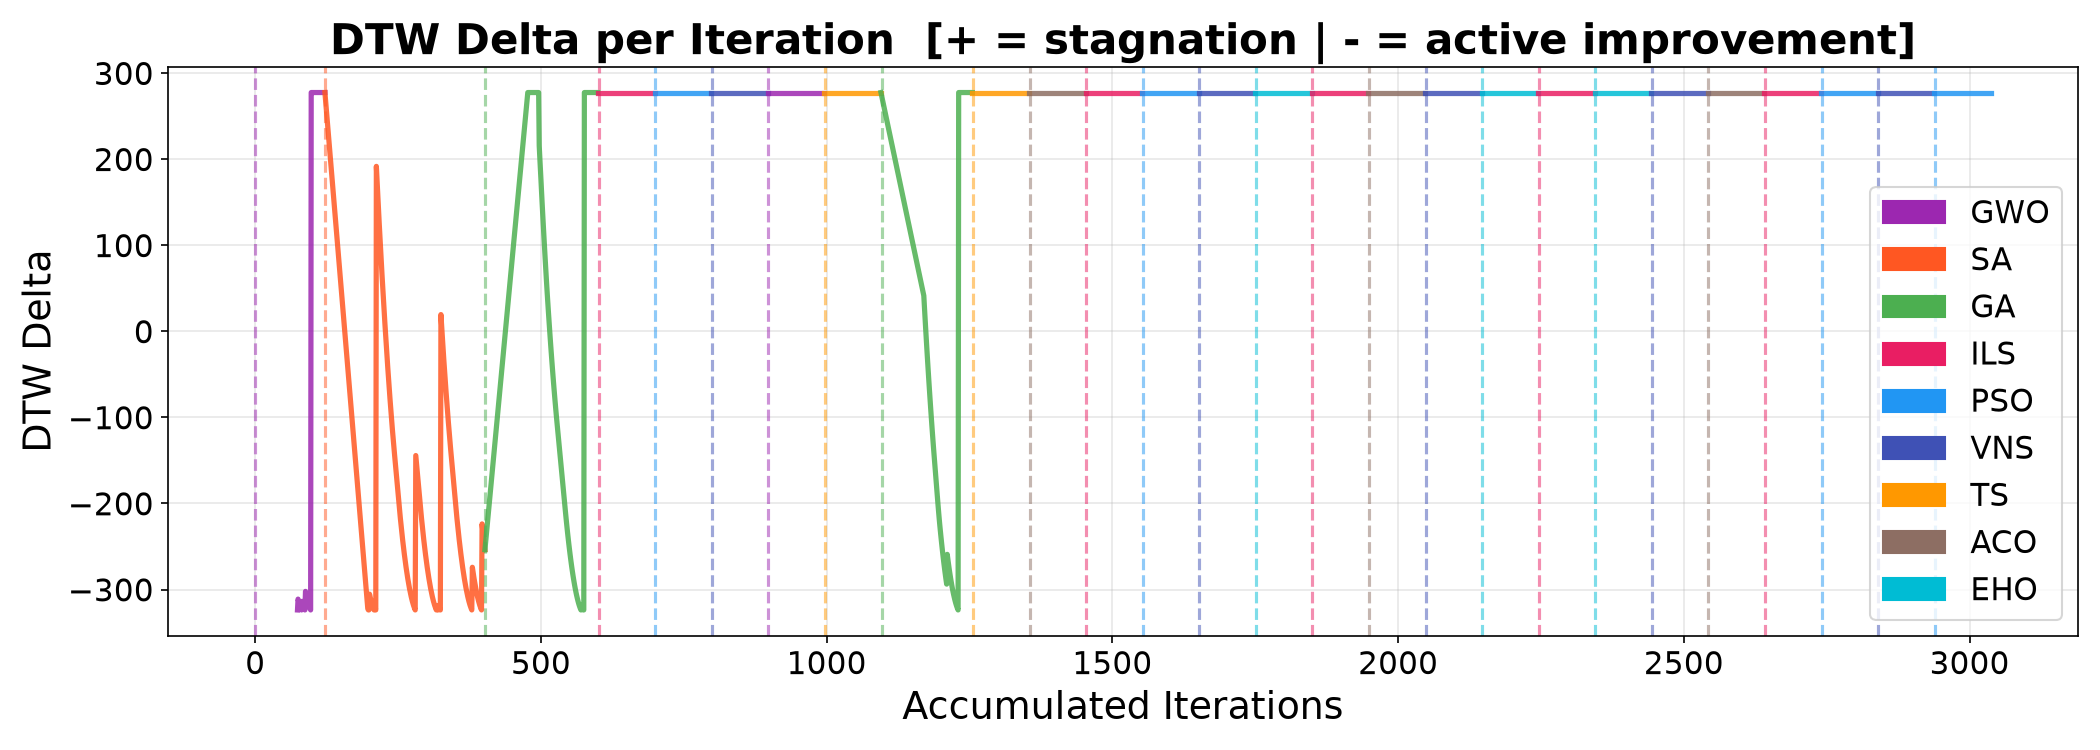
\includegraphics[width=0.32\textwidth]{imagenes_paper/mkp_dtw_3k_mknapcb1_delta.png}}
\caption{Diagnostic suite for instance \textbf{mknapcb1} ($n=100$, $m=5$) under the DTW framework with $T_{\max}=3{,}000$: (a)~final-fitness distribution over $N=31$ runs; (b)~convergence trajectory of the best run; (c)~elastic warping profile $\Delta$.}
\label{fig:mkp-best-cb1}
\end{figure}

% --- mknapcb2: DDTW, 3,000 iterations ---
\begin{figure}[htbp]
\centering
\subfloat[Metaheuristic comparison.]{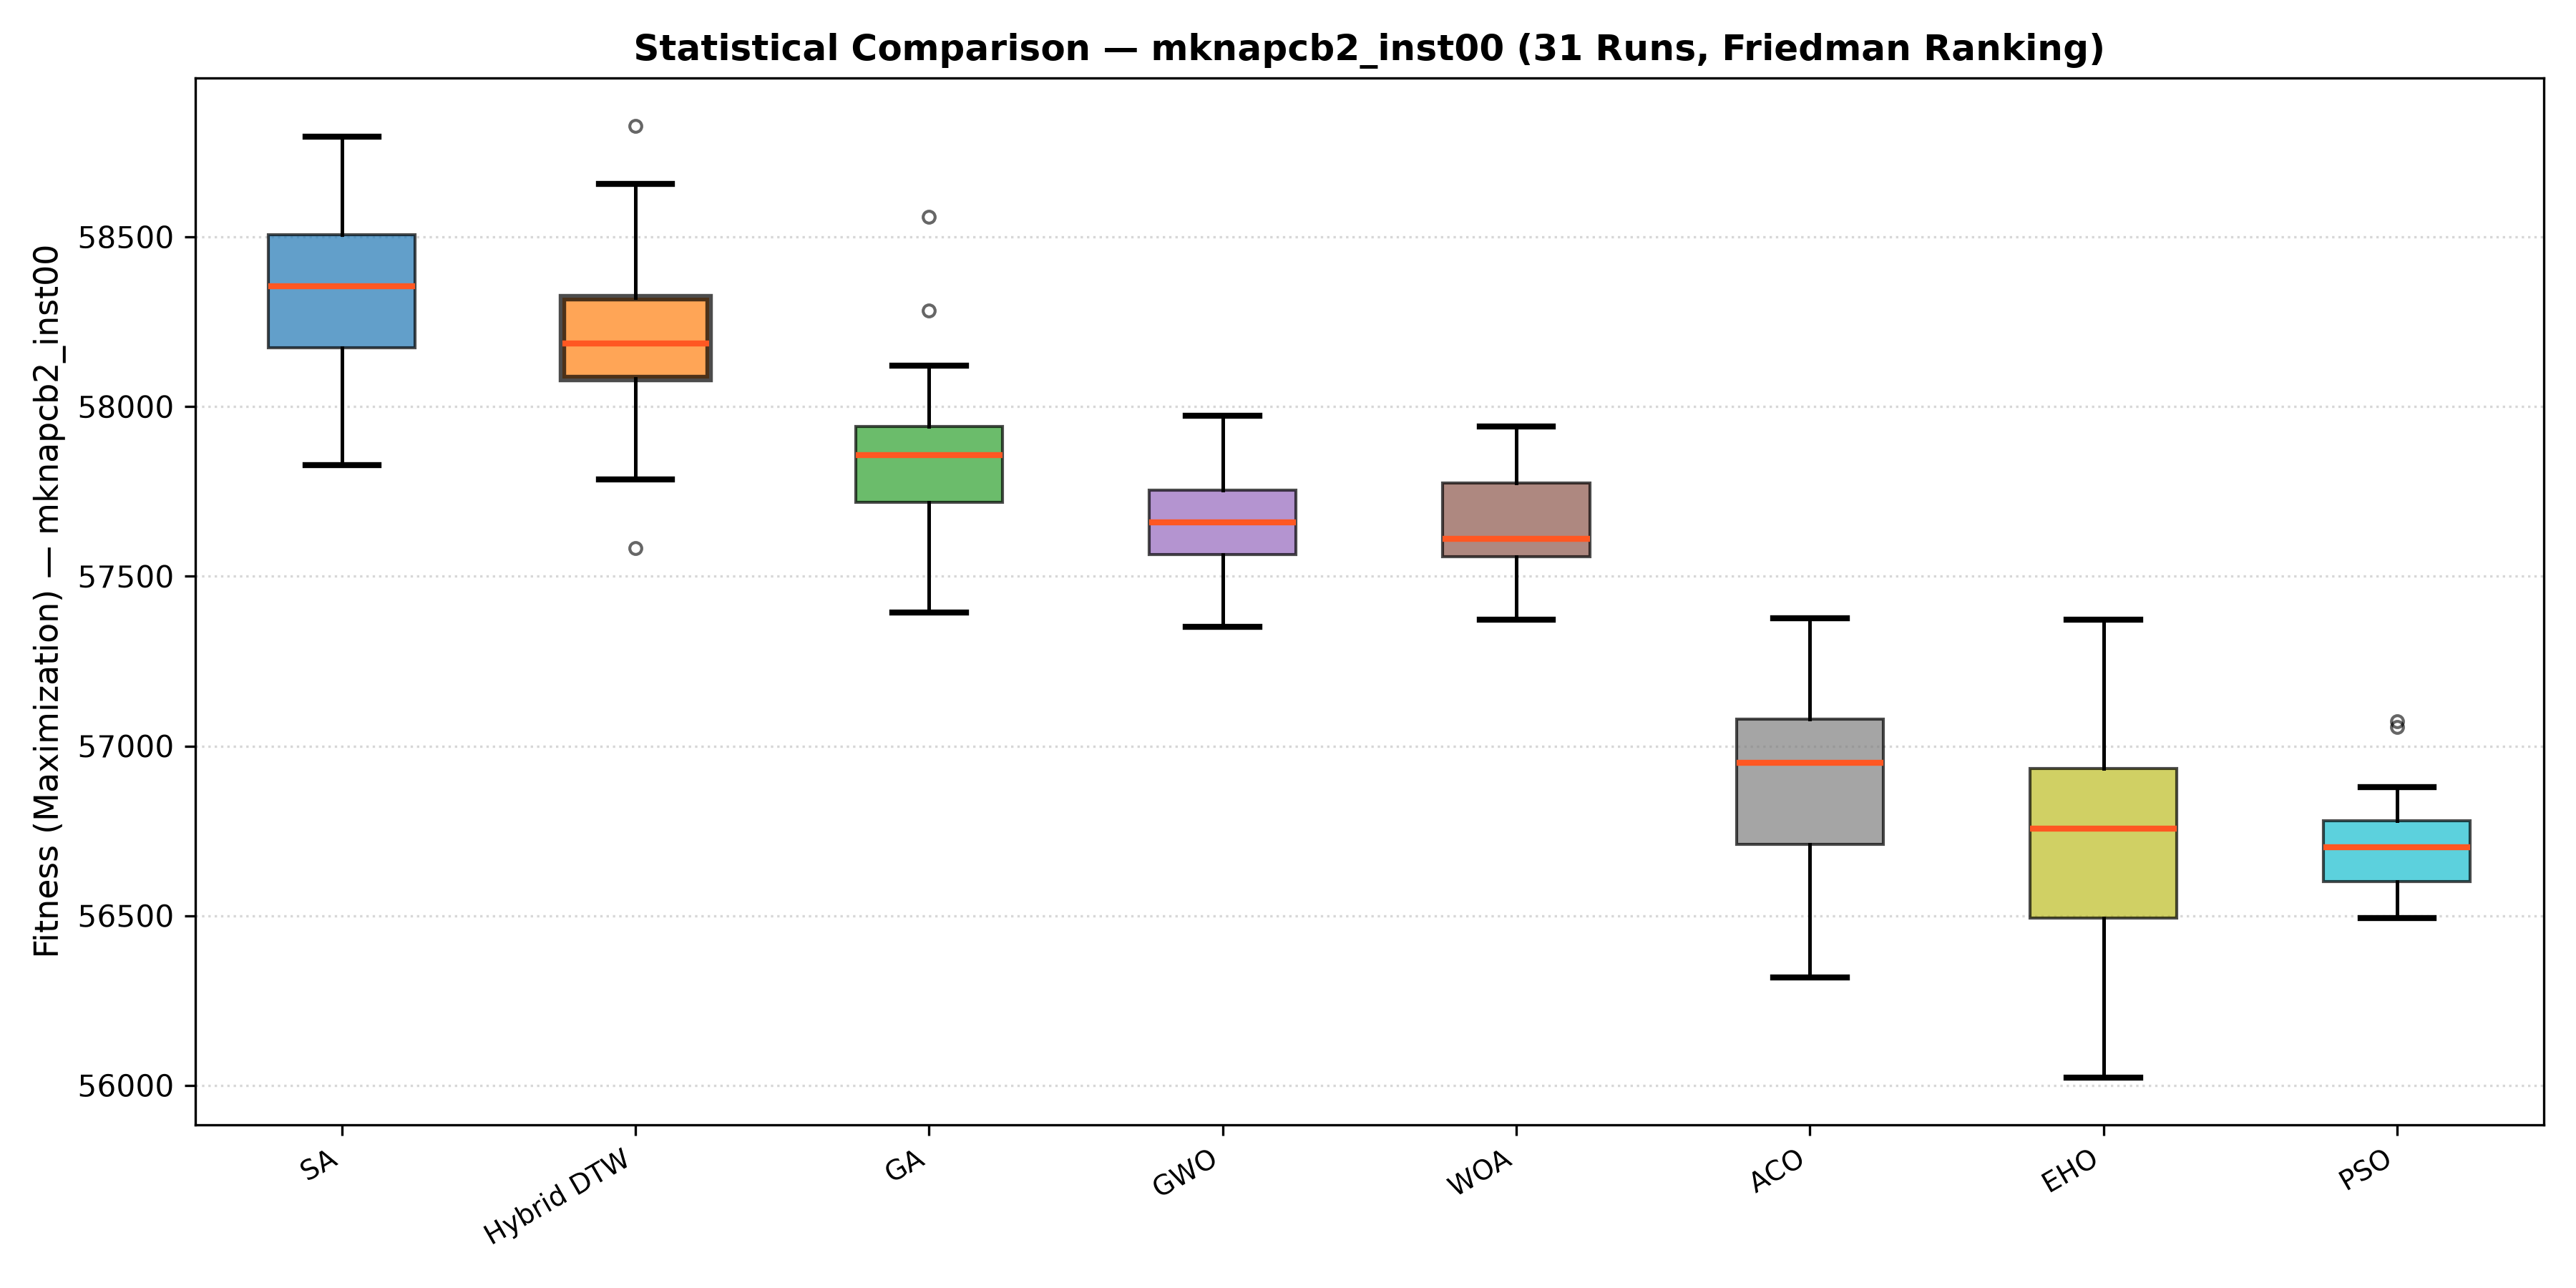
\includegraphics[width=0.32\textwidth]{imagenes_paper/mkp_ddtw_3k_mknapcb2_comparativo_mh.png}}\hfill
\subfloat[Best-run convergence.]{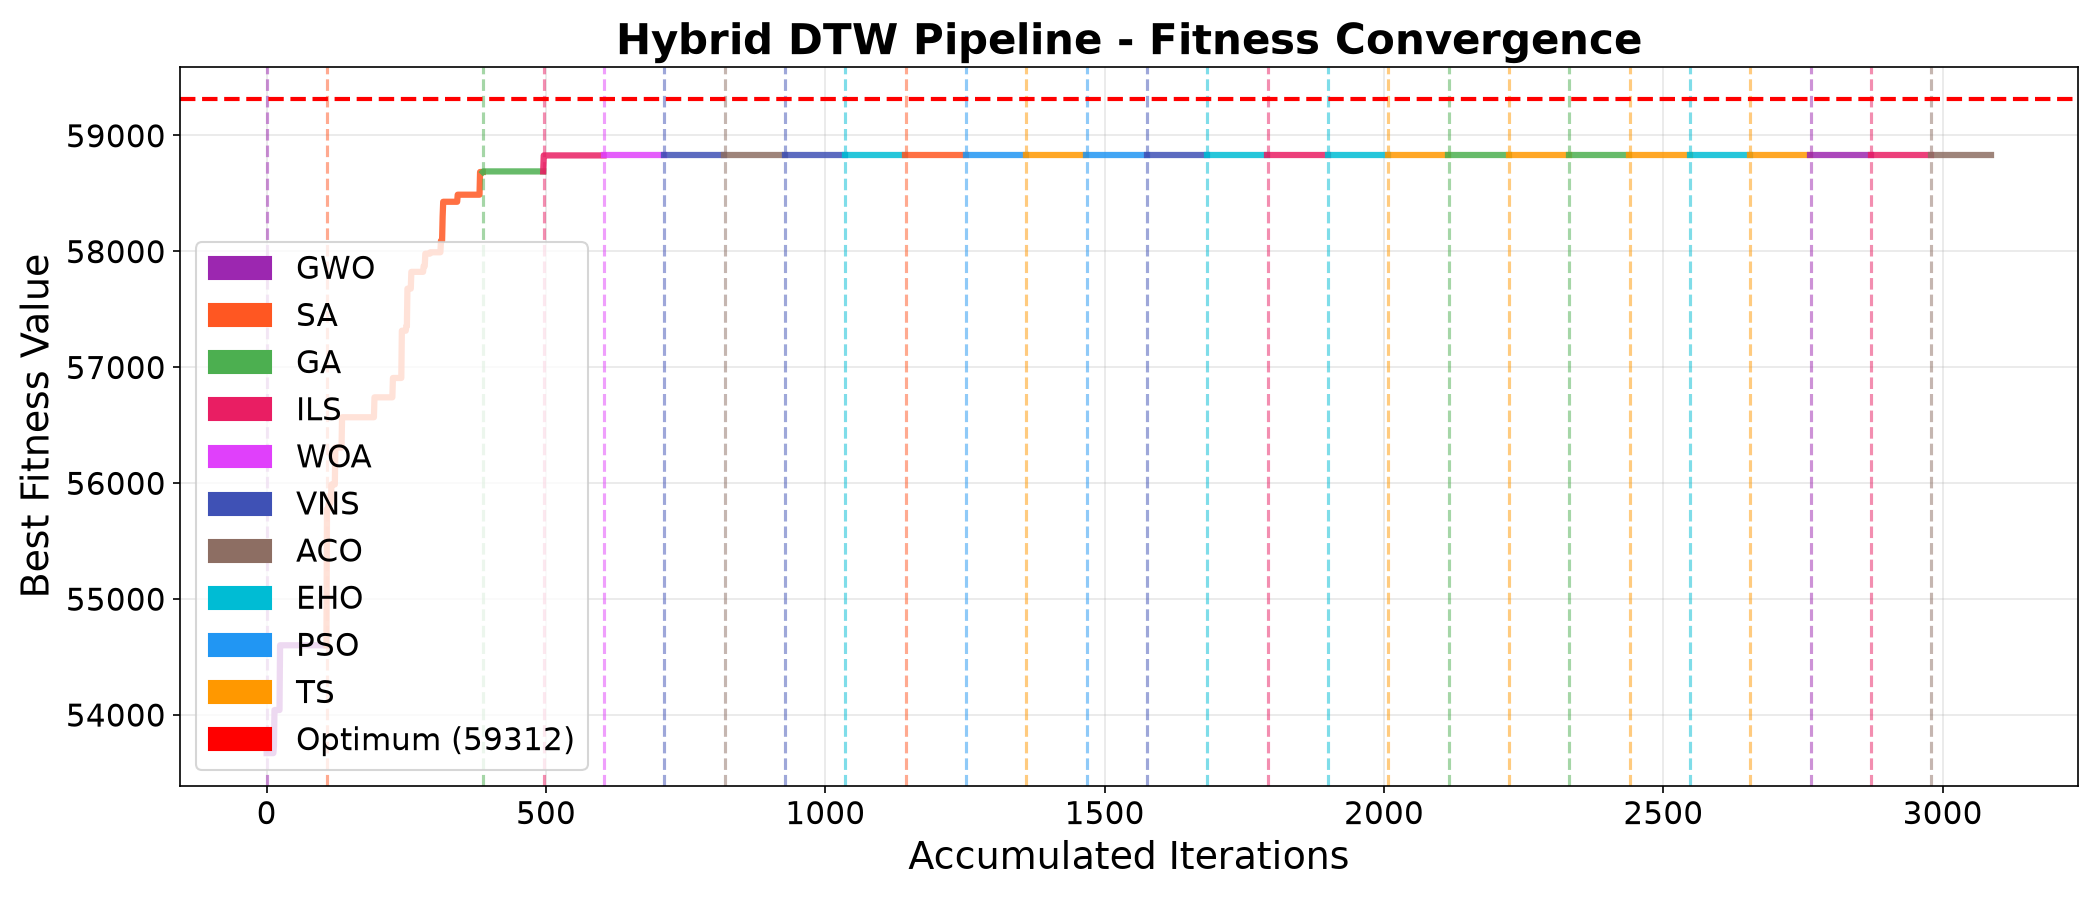
\includegraphics[width=0.32\textwidth]{imagenes_paper/mkp_ddtw_3k_mknapcb2_convergencia.png}}\hfill
\subfloat[Elastic metric $\Delta=D_1-D_2$.]{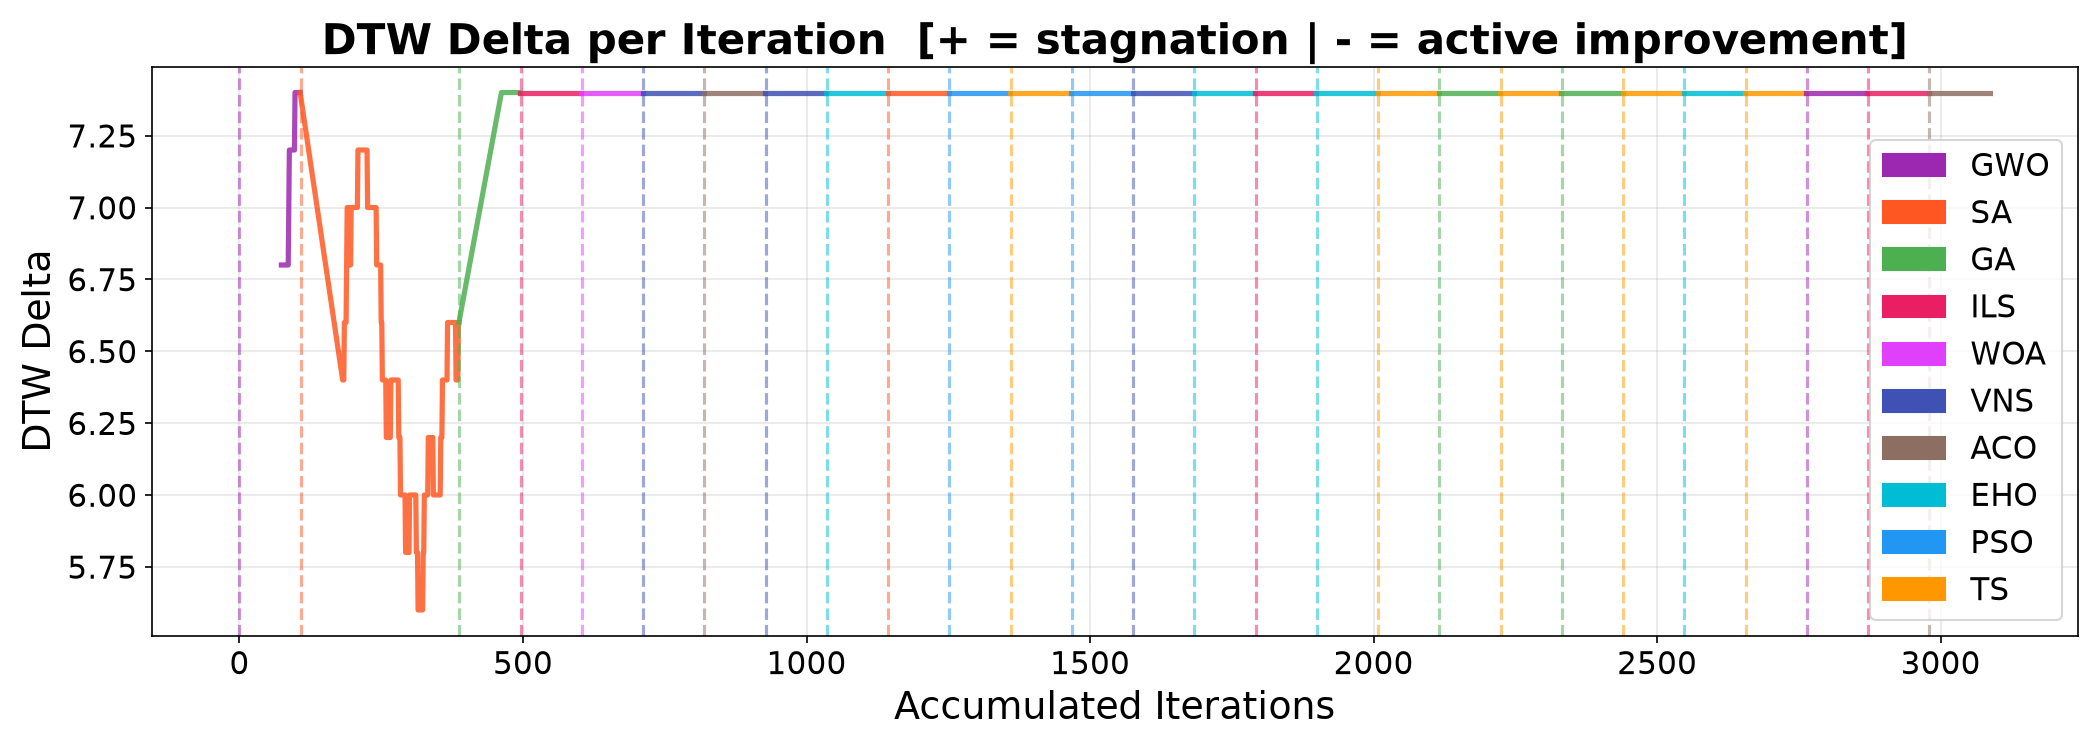
\includegraphics[width=0.32\textwidth]{imagenes_paper/mkp_ddtw_3k_mknapcb2_delta.png}}
\caption{Diagnostic suite for instance \textbf{mknapcb2} ($n=250$, $m=5$) under the DDTW framework with $T_{\max}=3{,}000$: (a)~final-fitness distribution over $N=31$ runs; (b)~convergence trajectory of the best run; (c)~elastic warping profile $\Delta$.}
\label{fig:mkp-best-cb2}
\end{figure}

% --- mknapcb3: DTW, 3,000 iterations ---
\begin{figure}[htbp]
\centering
\subfloat[Metaheuristic comparison.]{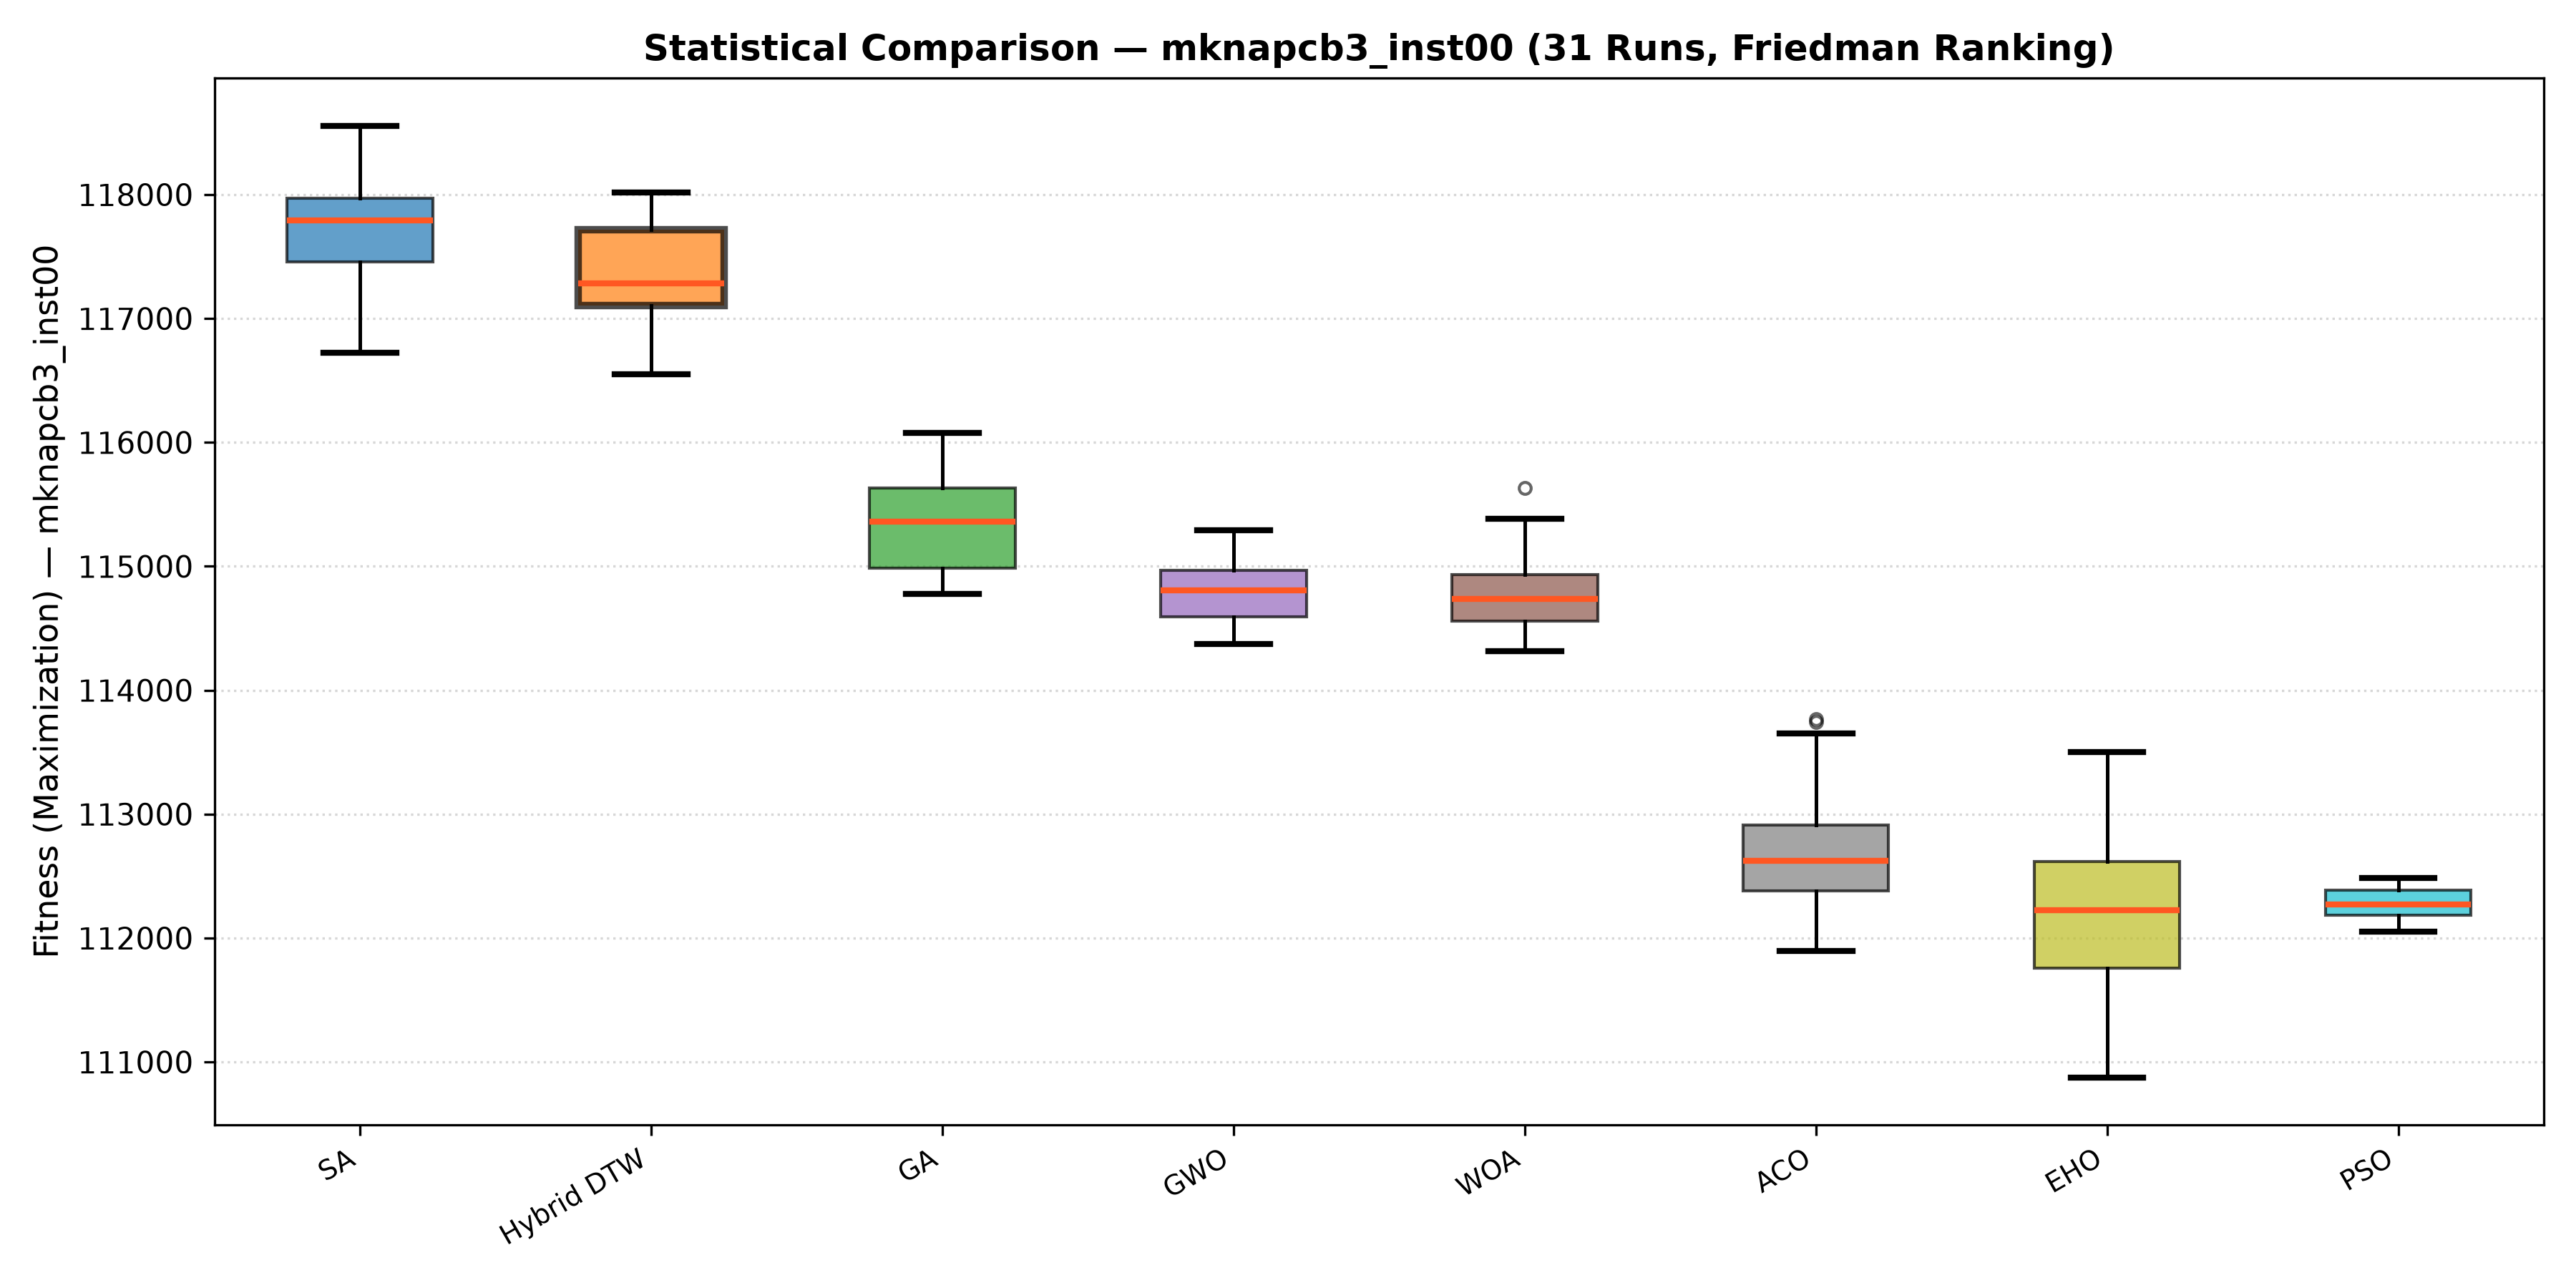
\includegraphics[width=0.32\textwidth]{imagenes_paper/mkp_dtw_3k_mknapcb3_comparativo_mh.png}}\hfill
\subfloat[Best-run convergence.]{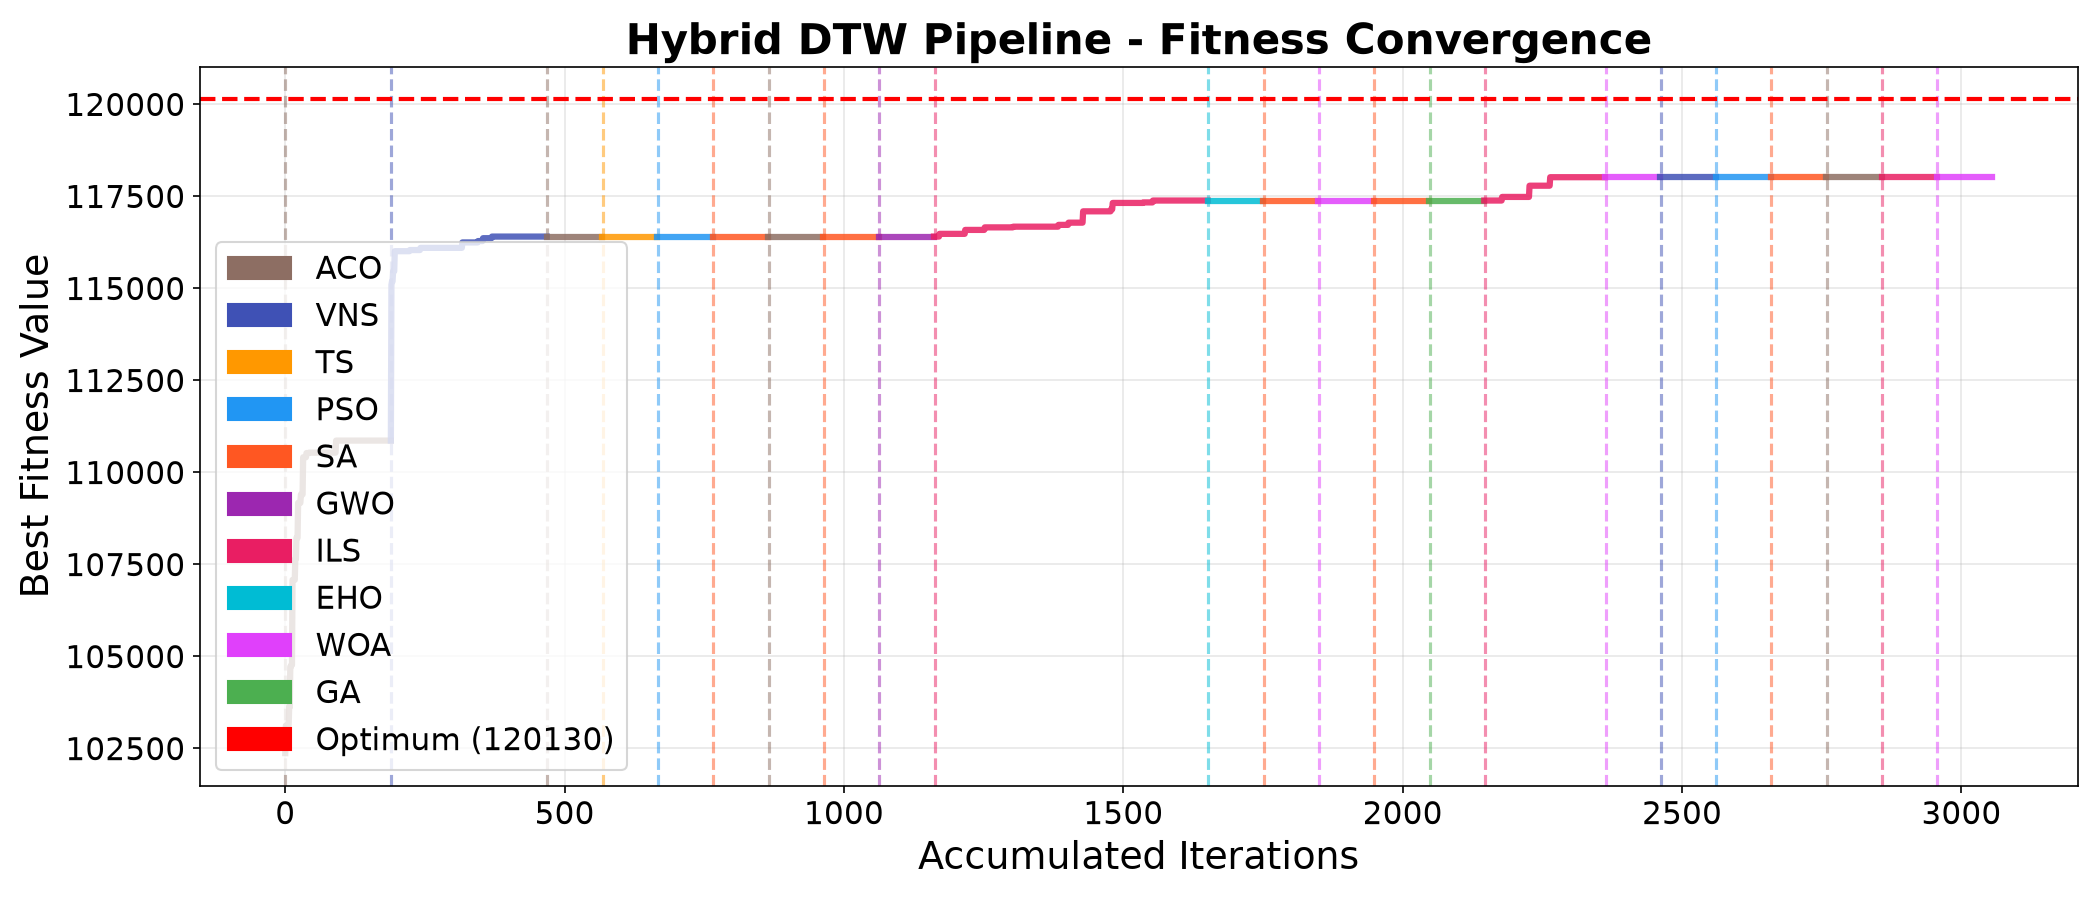
\includegraphics[width=0.32\textwidth]{imagenes_paper/mkp_dtw_3k_mknapcb3_convergencia.png}}\hfill
\subfloat[Elastic metric $\Delta=D_1-D_2$.]{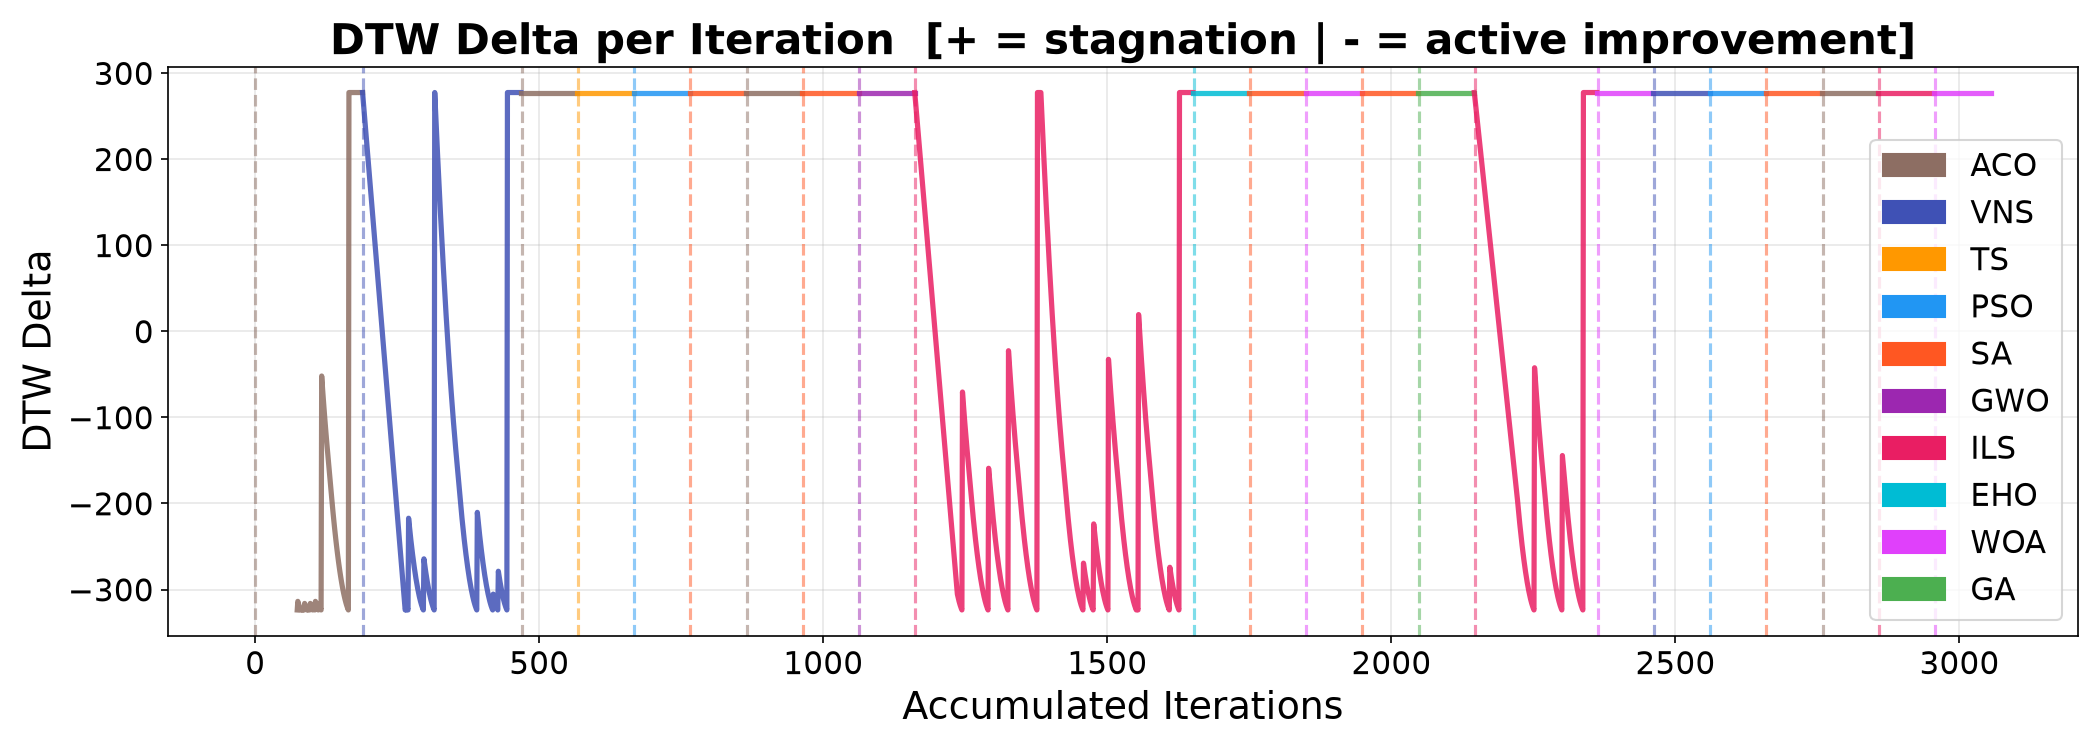
\includegraphics[width=0.32\textwidth]{imagenes_paper/mkp_dtw_3k_mknapcb3_delta.png}}
\caption{Diagnostic suite for instance \textbf{mknapcb3} ($n=500$, $m=5$) under the DTW framework with $T_{\max}=3{,}000$: (a)~final-fitness distribution over $N=31$ runs; (b)~convergence trajectory of the best run; (c)~elastic warping profile $\Delta$.}
\label{fig:mkp-best-cb3}
\end{figure}

% --- mknapcb4: DTW, 3,000 iterations ---
\begin{figure}[htbp]
\centering
\subfloat[Metaheuristic comparison.]{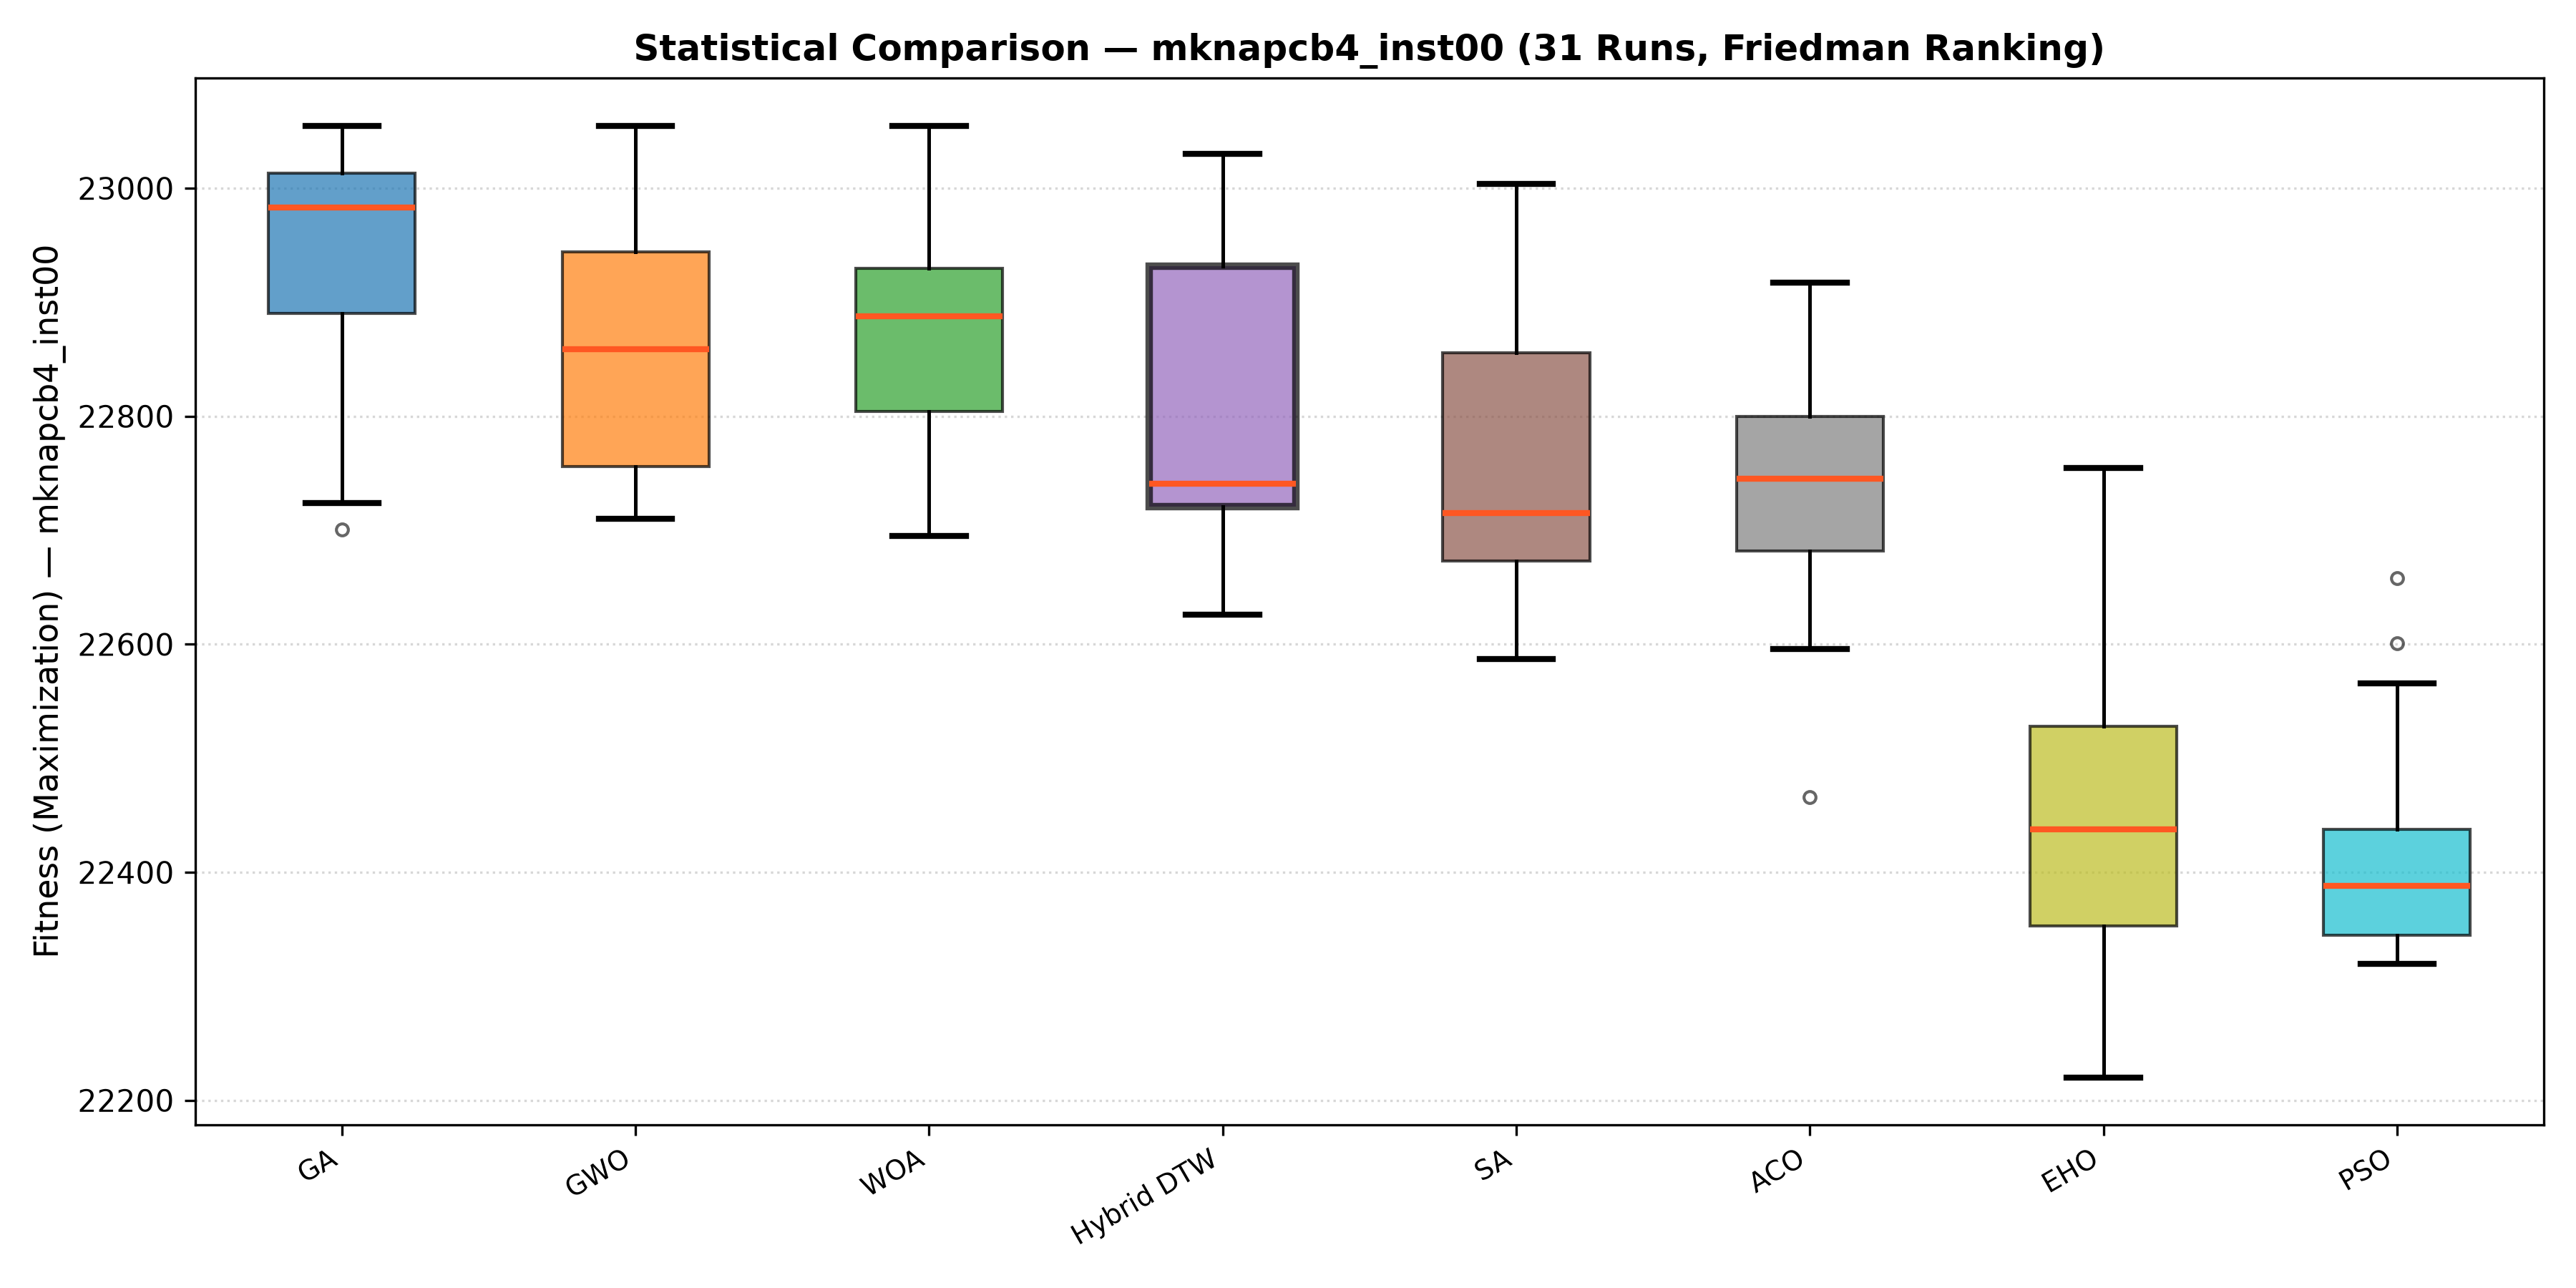
\includegraphics[width=0.32\textwidth]{imagenes_paper/mkp_dtw_3k_mknapcb4_comparativo_mh.png}}\hfill
\subfloat[Best-run convergence.]{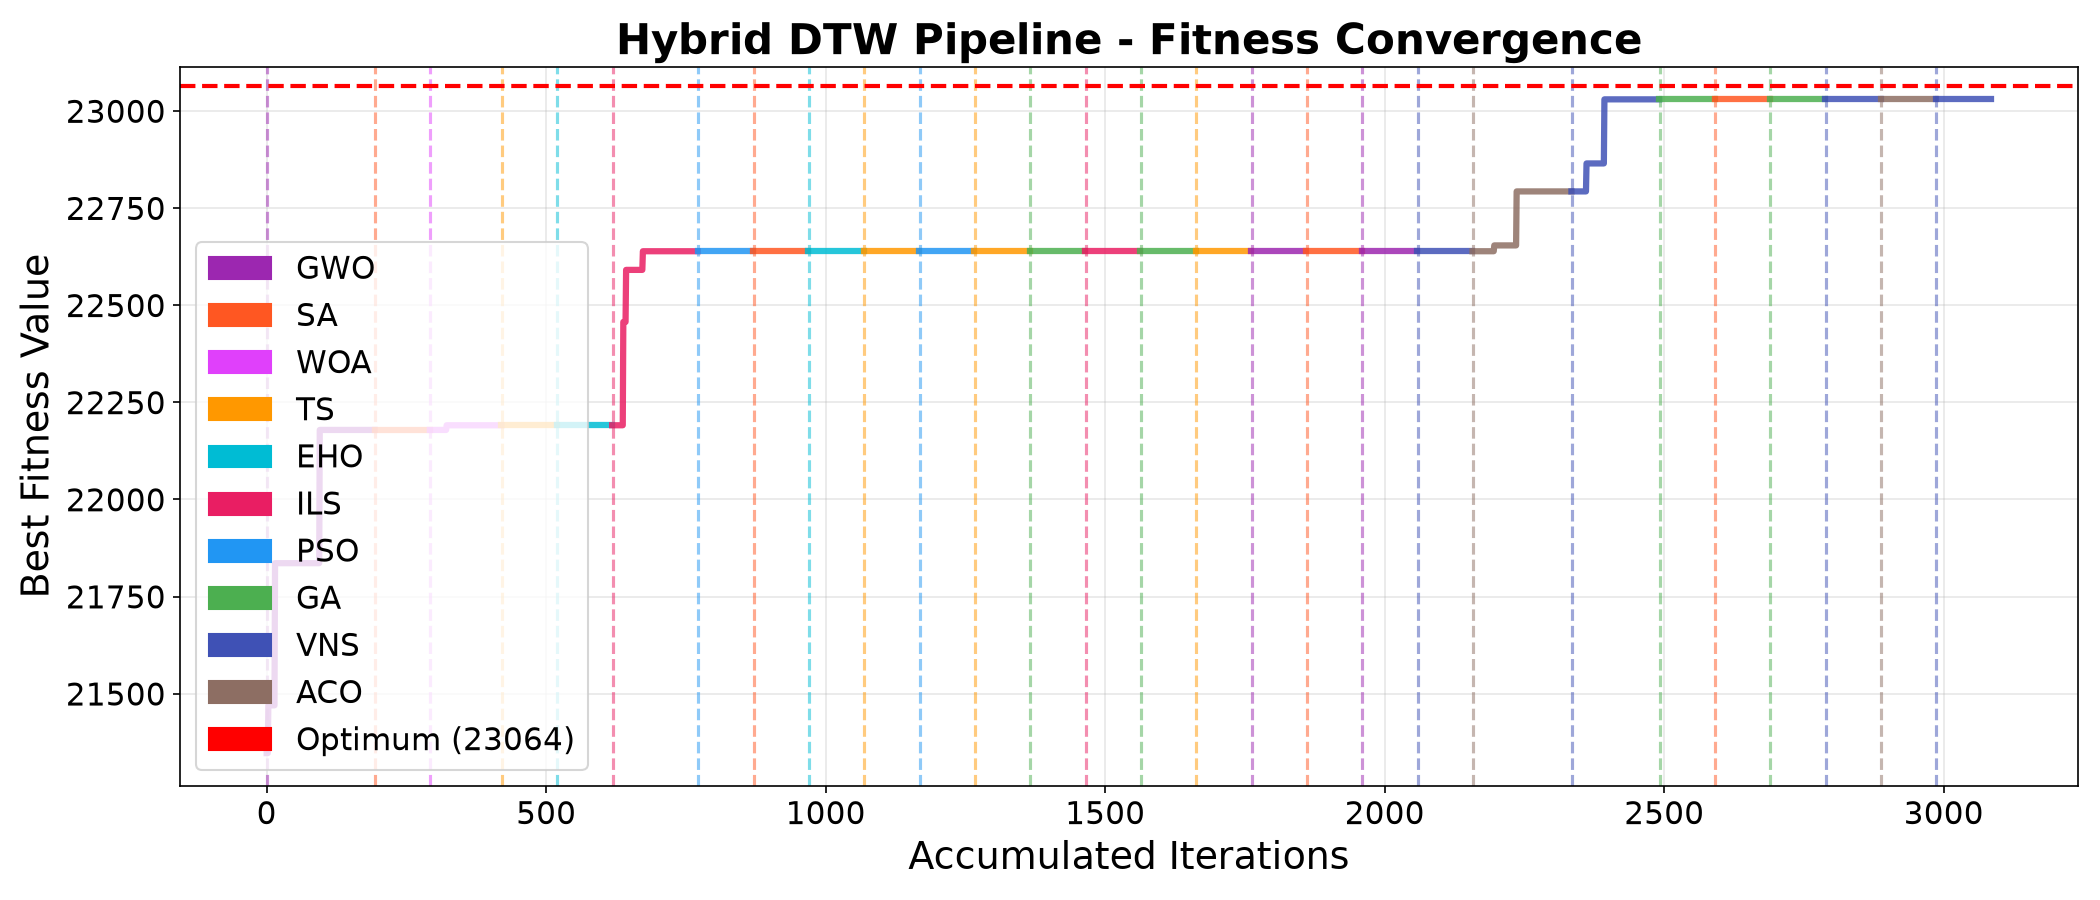
\includegraphics[width=0.32\textwidth]{imagenes_paper/mkp_dtw_3k_mknapcb4_convergencia.png}}\hfill
\subfloat[Elastic metric $\Delta=D_1-D_2$.]{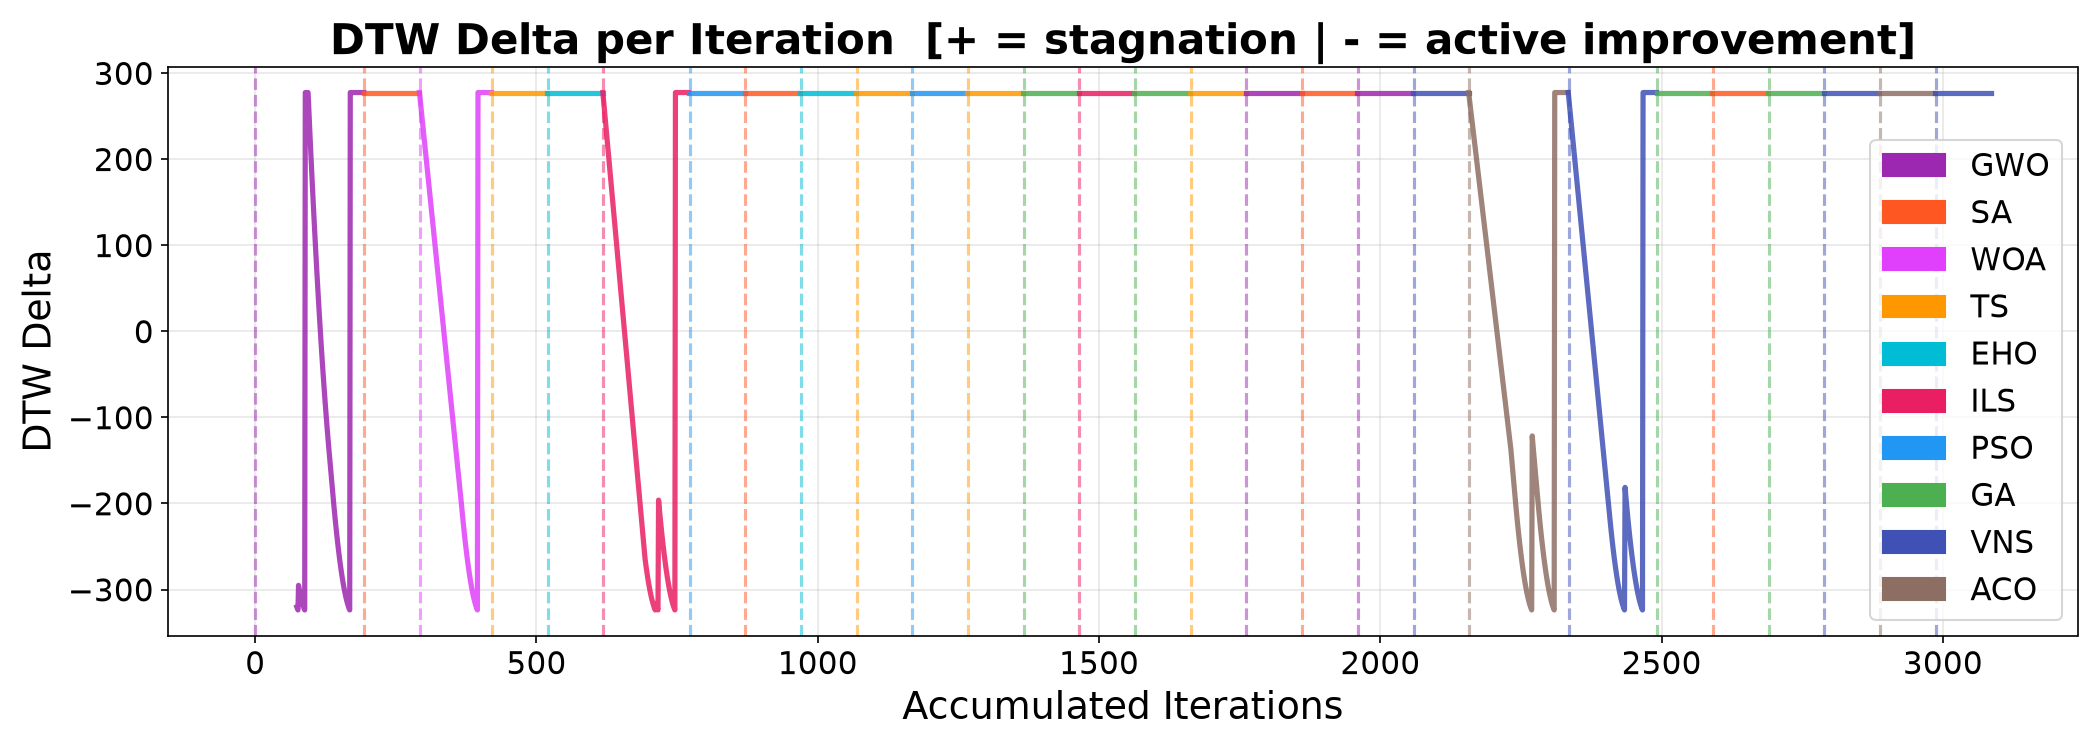
\includegraphics[width=0.32\textwidth]{imagenes_paper/mkp_dtw_3k_mknapcb4_delta.png}}
\caption{Diagnostic suite for instance \textbf{mknapcb4} ($n=100$, $m=10$) under the DTW framework with $T_{\max}=3{,}000$: (a)~final-fitness distribution over $N=31$ runs; (b)~convergence trajectory of the best run; (c)~elastic warping profile $\Delta$.}
\label{fig:mkp-best-cb4}
\end{figure}

% --- mknapcb5: DTW, 3,000 iterations ---
\begin{figure}[htbp]
\centering
\subfloat[Metaheuristic comparison.]{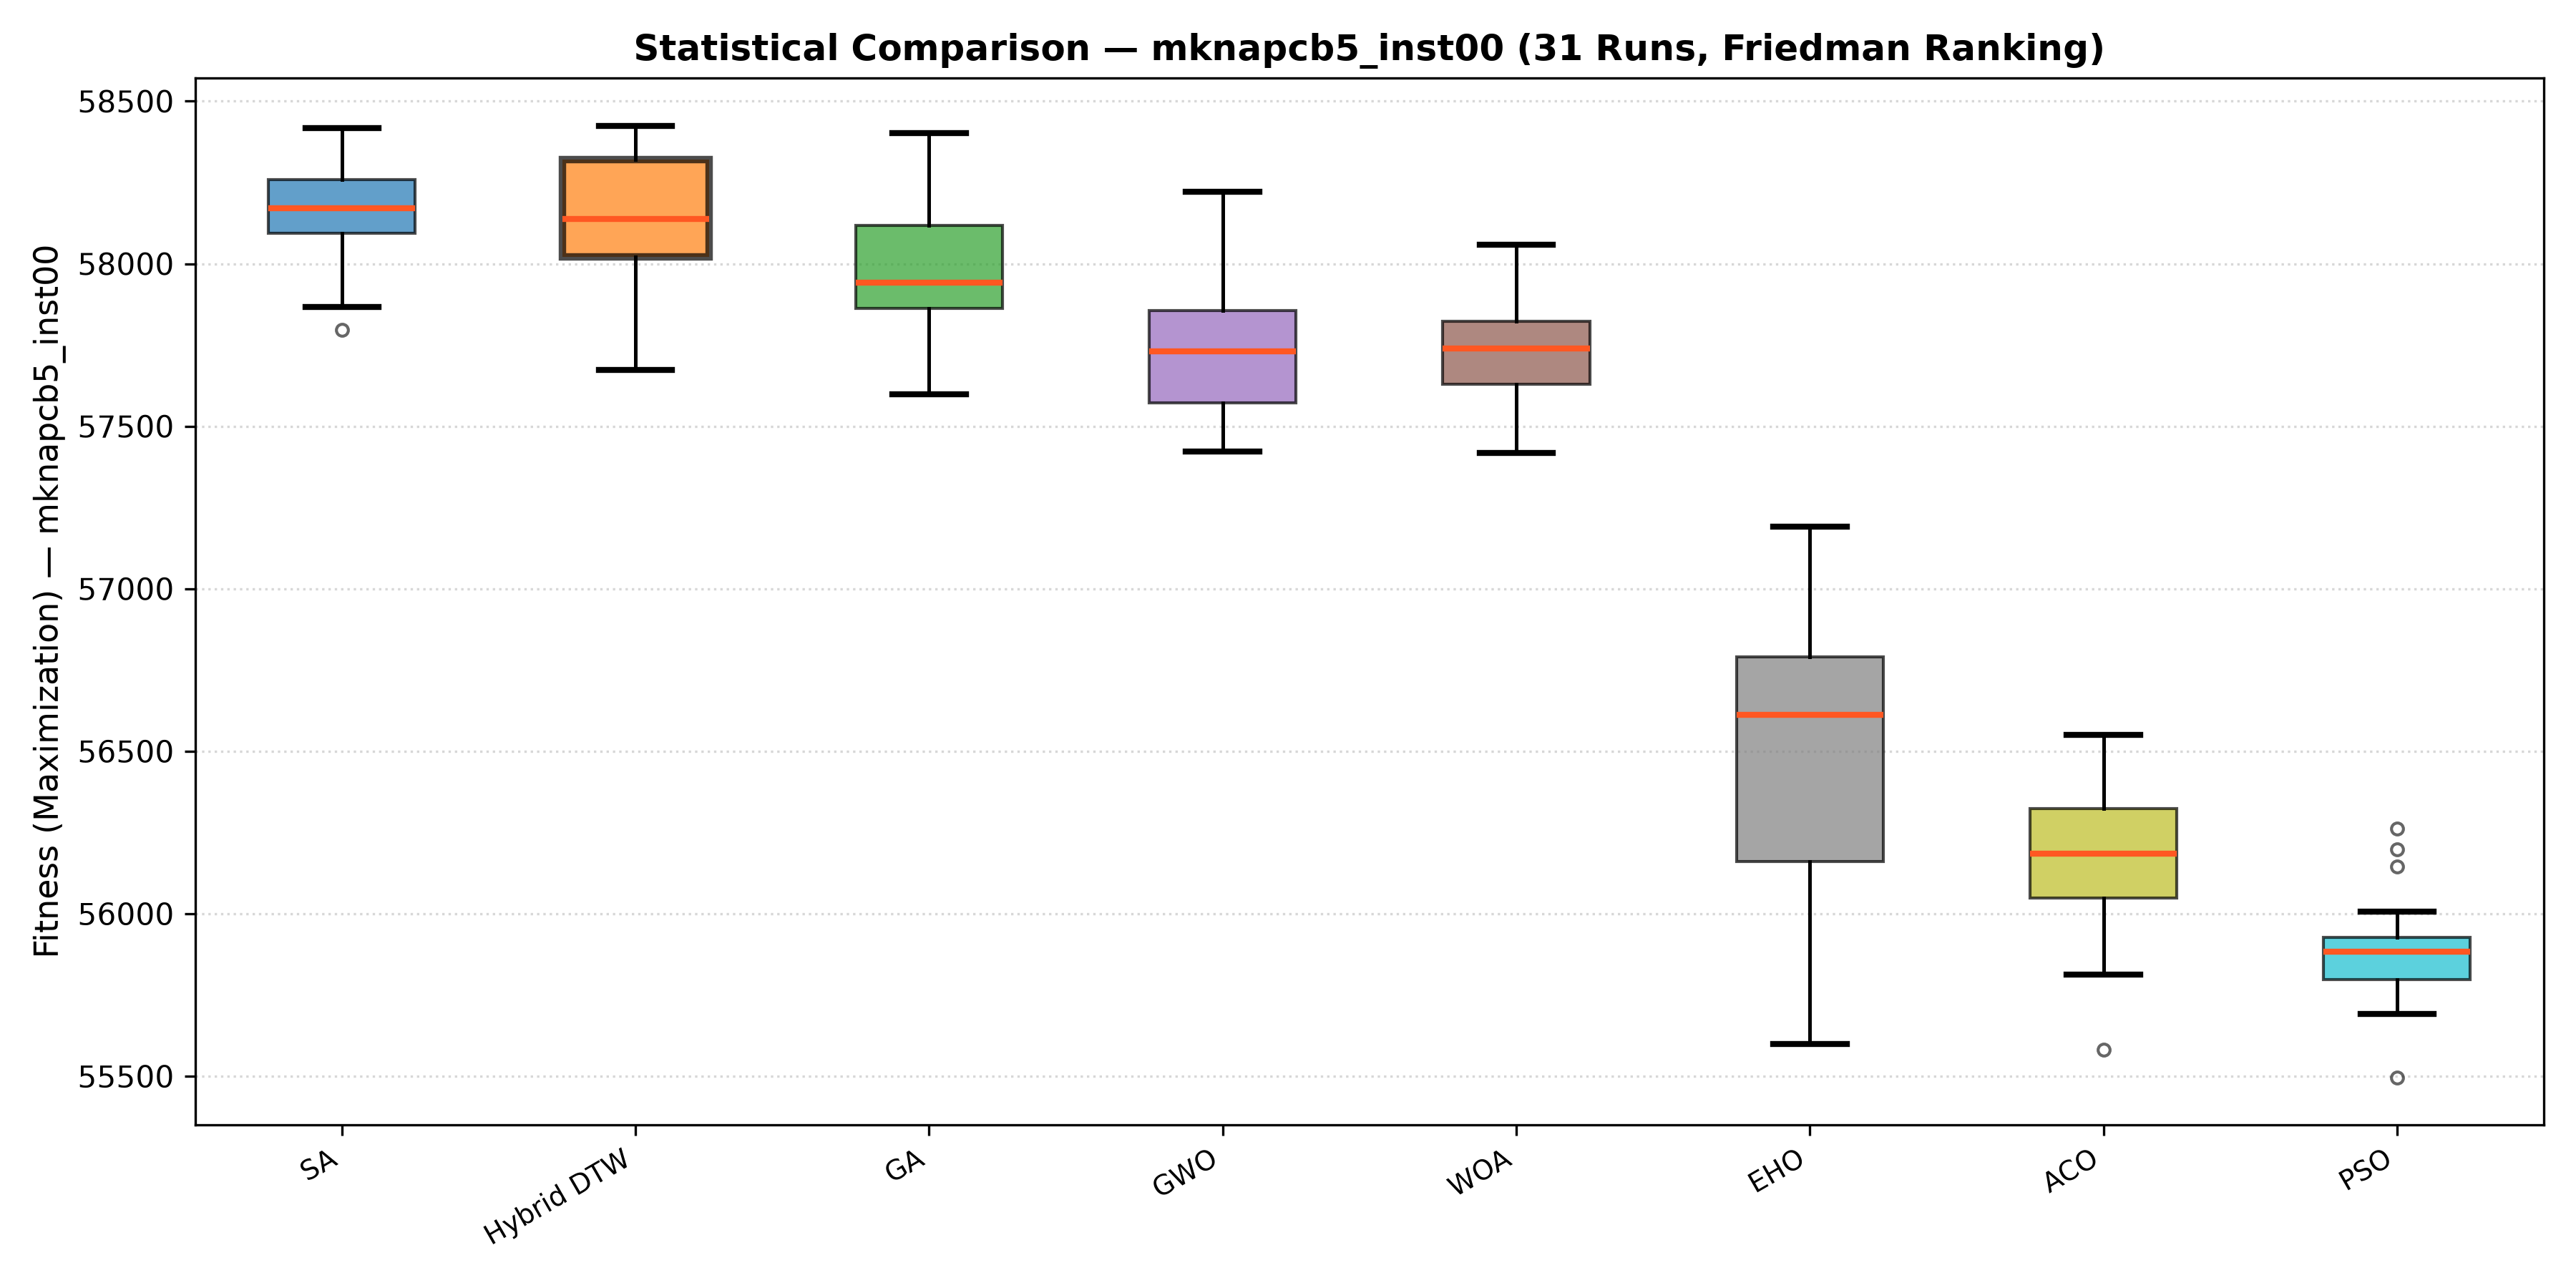
\includegraphics[width=0.32\textwidth]{imagenes_paper/mkp_dtw_3k_mknapcb5_comparativo_mh.png}}\hfill
\subfloat[Best-run convergence.]{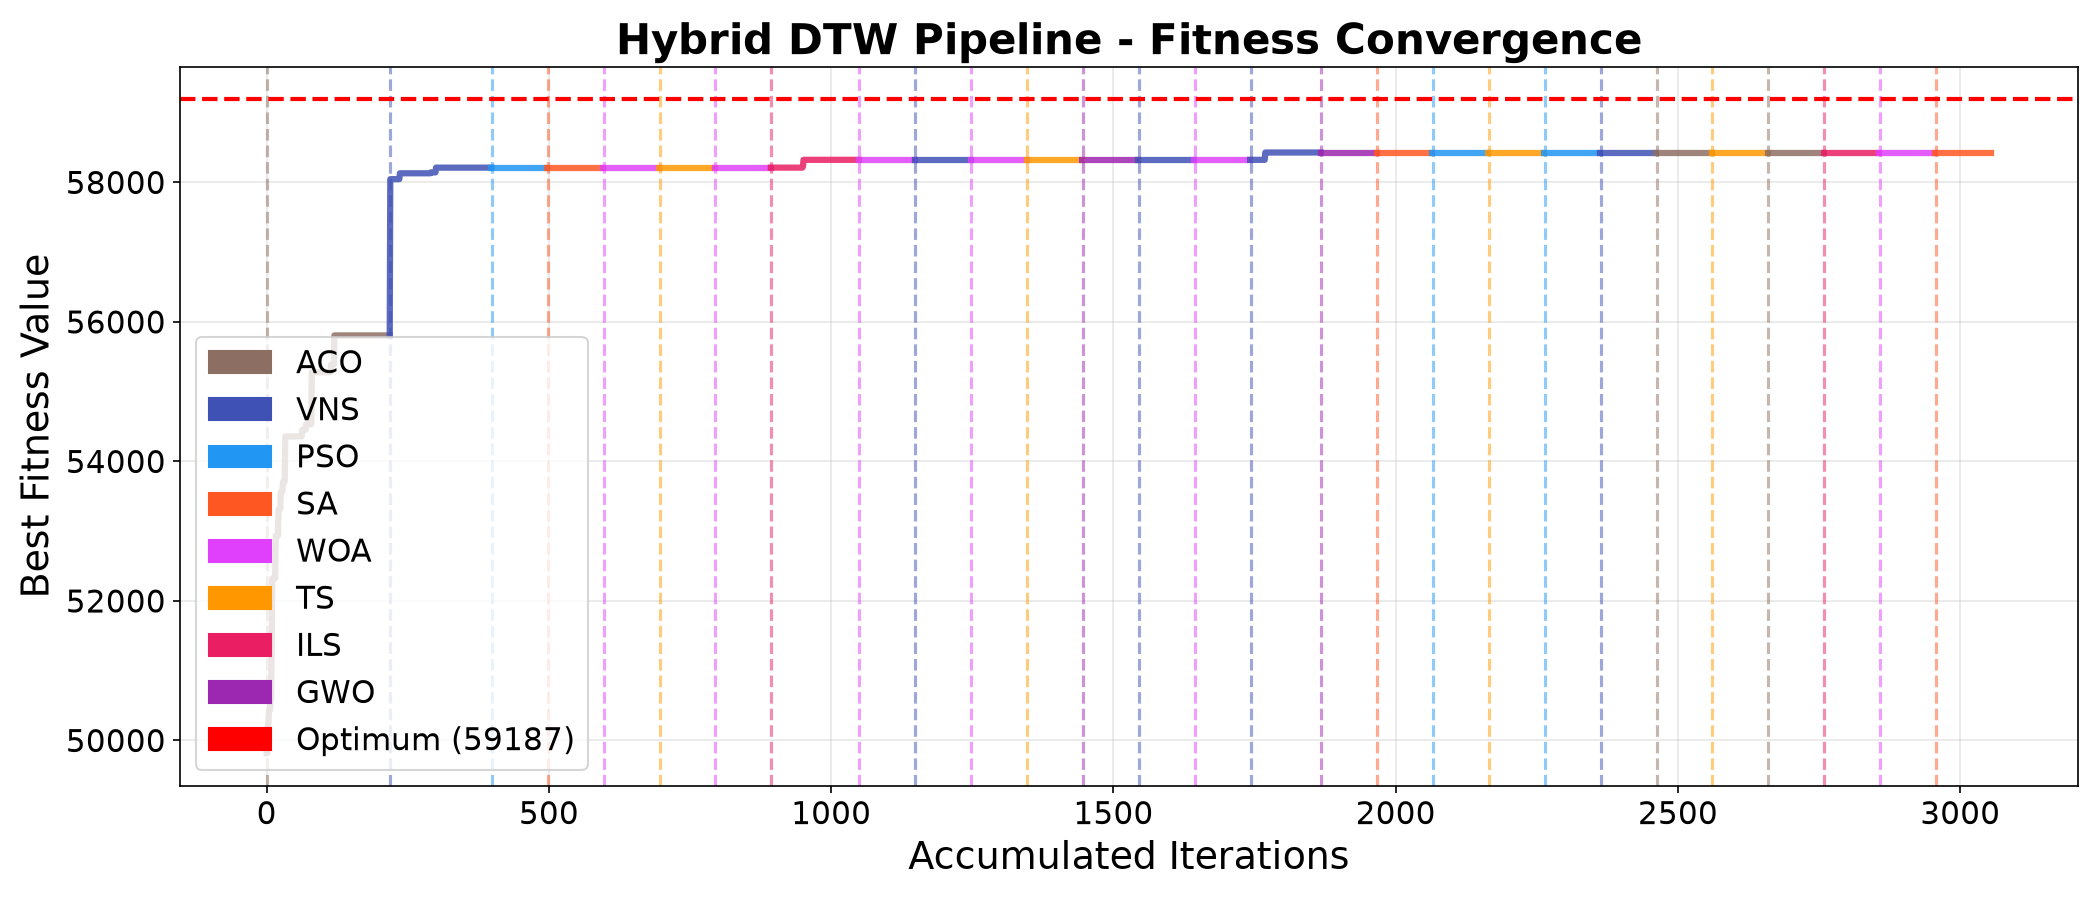
\includegraphics[width=0.32\textwidth]{imagenes_paper/mkp_dtw_3k_mknapcb5_convergencia.png}}\hfill
\subfloat[Elastic metric $\Delta=D_1-D_2$.]{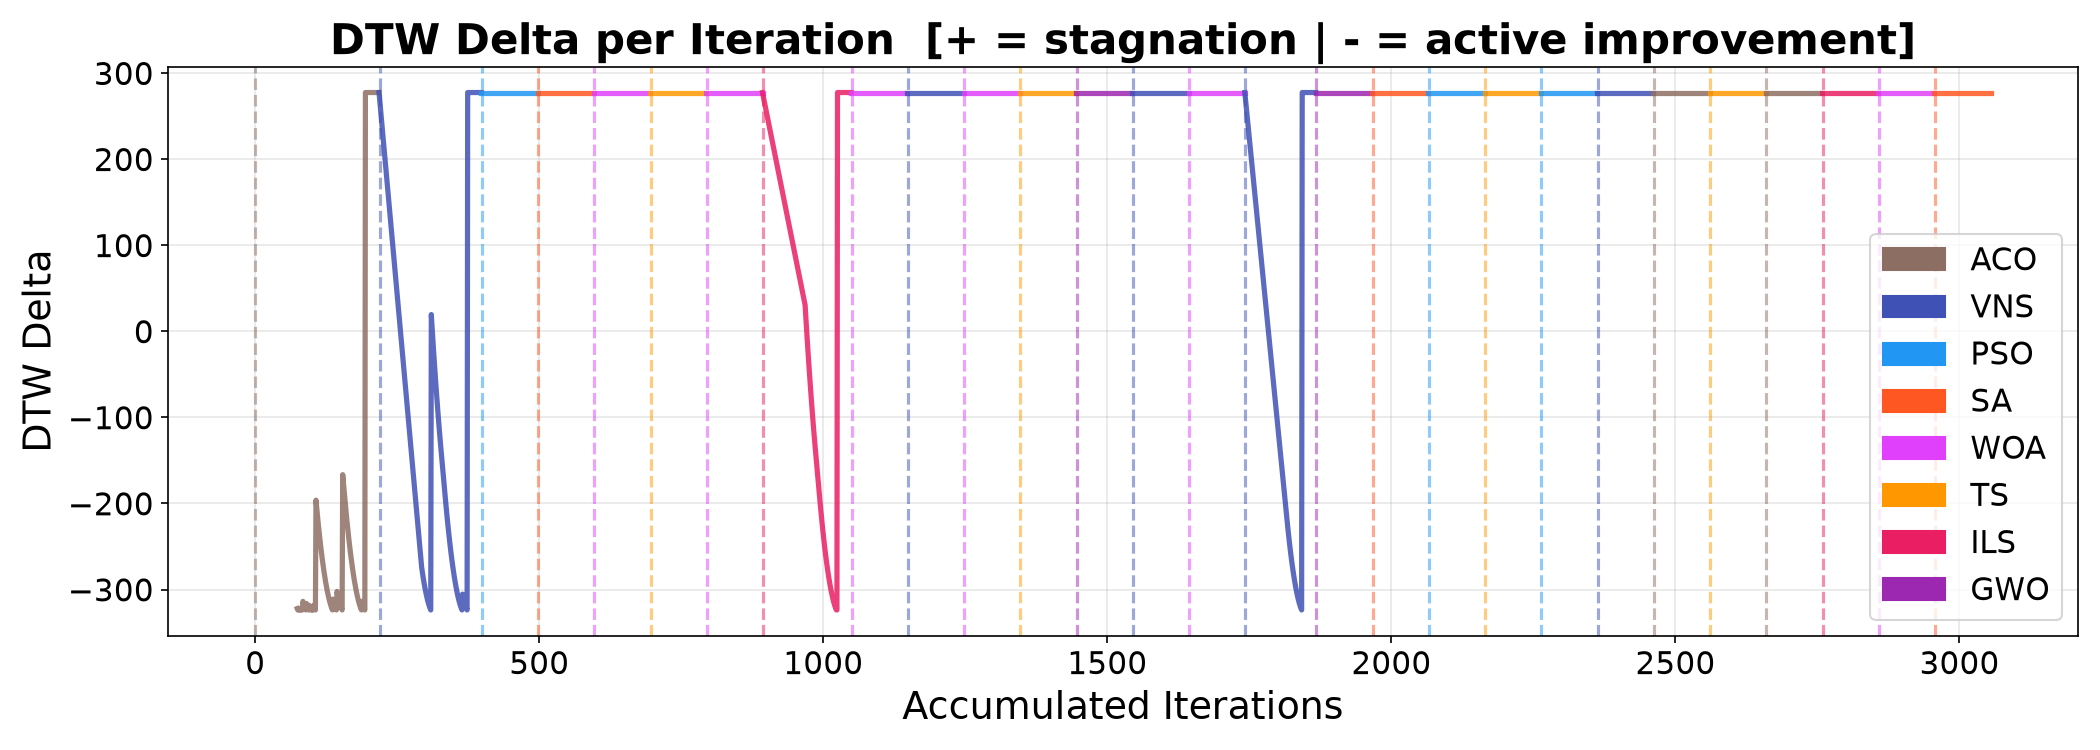
\includegraphics[width=0.32\textwidth]{imagenes_paper/mkp_dtw_3k_mknapcb5_delta.png}}
\caption{Diagnostic suite for instance \textbf{mknapcb5} ($n=250$, $m=10$) under the DTW framework with $T_{\max}=3{,}000$: (a)~final-fitness distribution over $N=31$ runs; (b)~convergence trajectory of the best run; (c)~elastic warping profile $\Delta$.}
\label{fig:mkp-best-cb5}
\end{figure}

% --- mknapcb6: DTW, 3,000 iterations ---
\begin{figure}[htbp]
\centering
\subfloat[Metaheuristic comparison.]{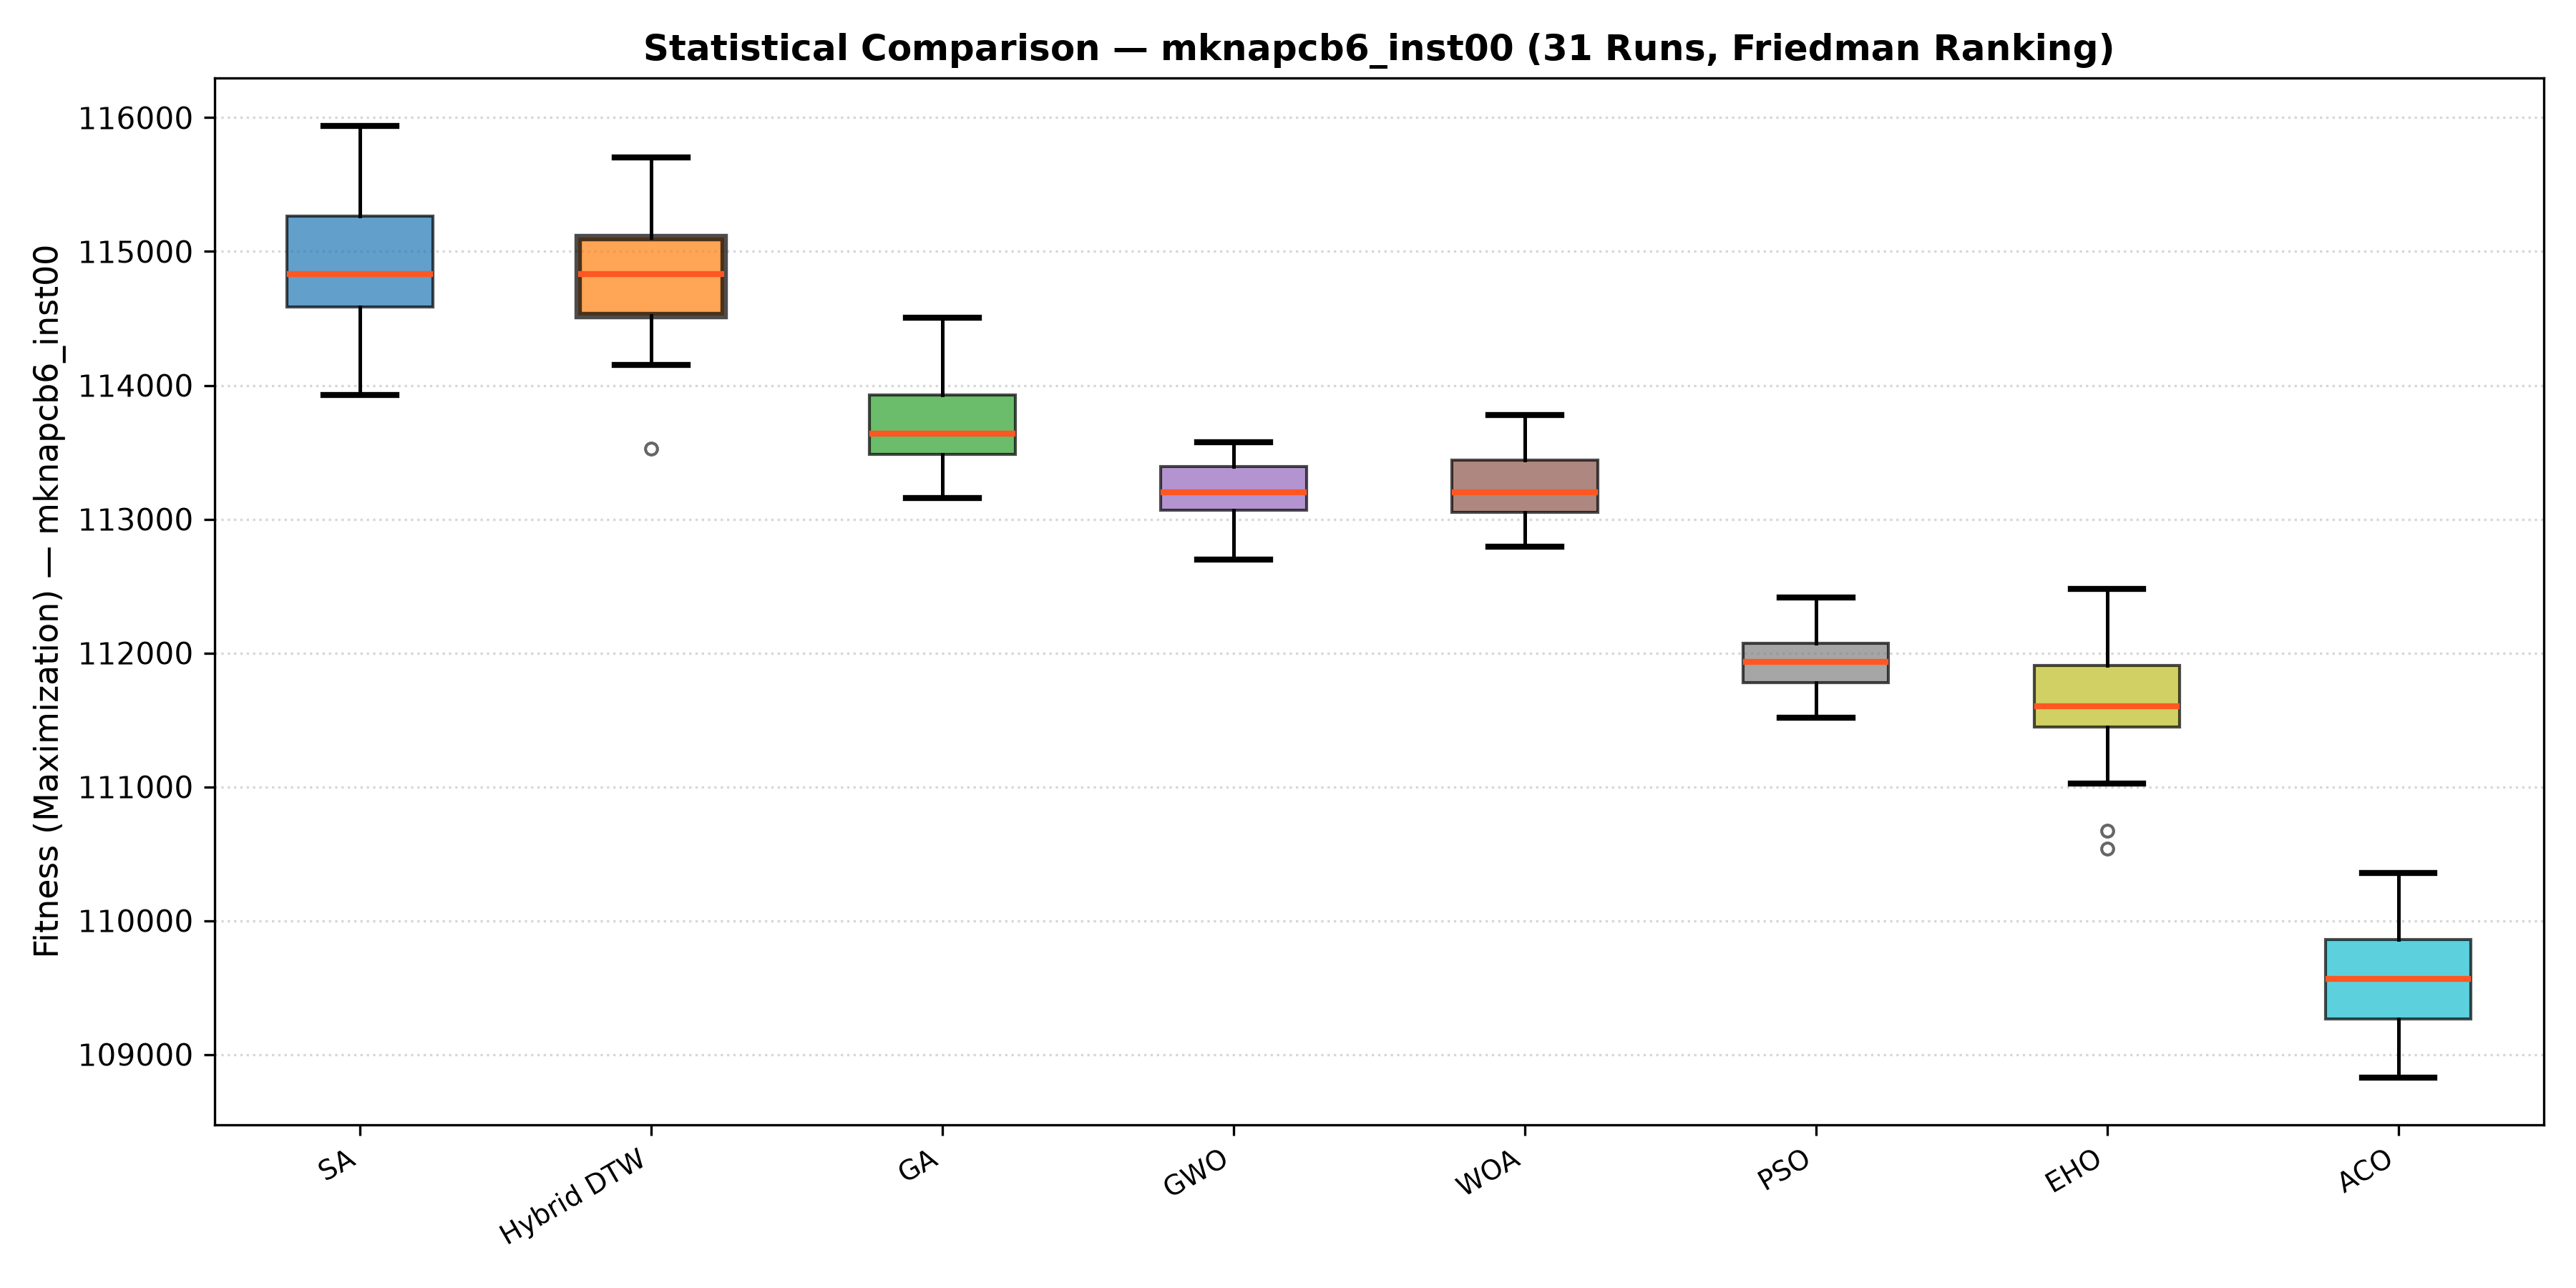
\includegraphics[width=0.32\textwidth]{imagenes_paper/mkp_dtw_3k_mknapcb6_comparativo_mh.png}}\hfill
\subfloat[Best-run convergence.]{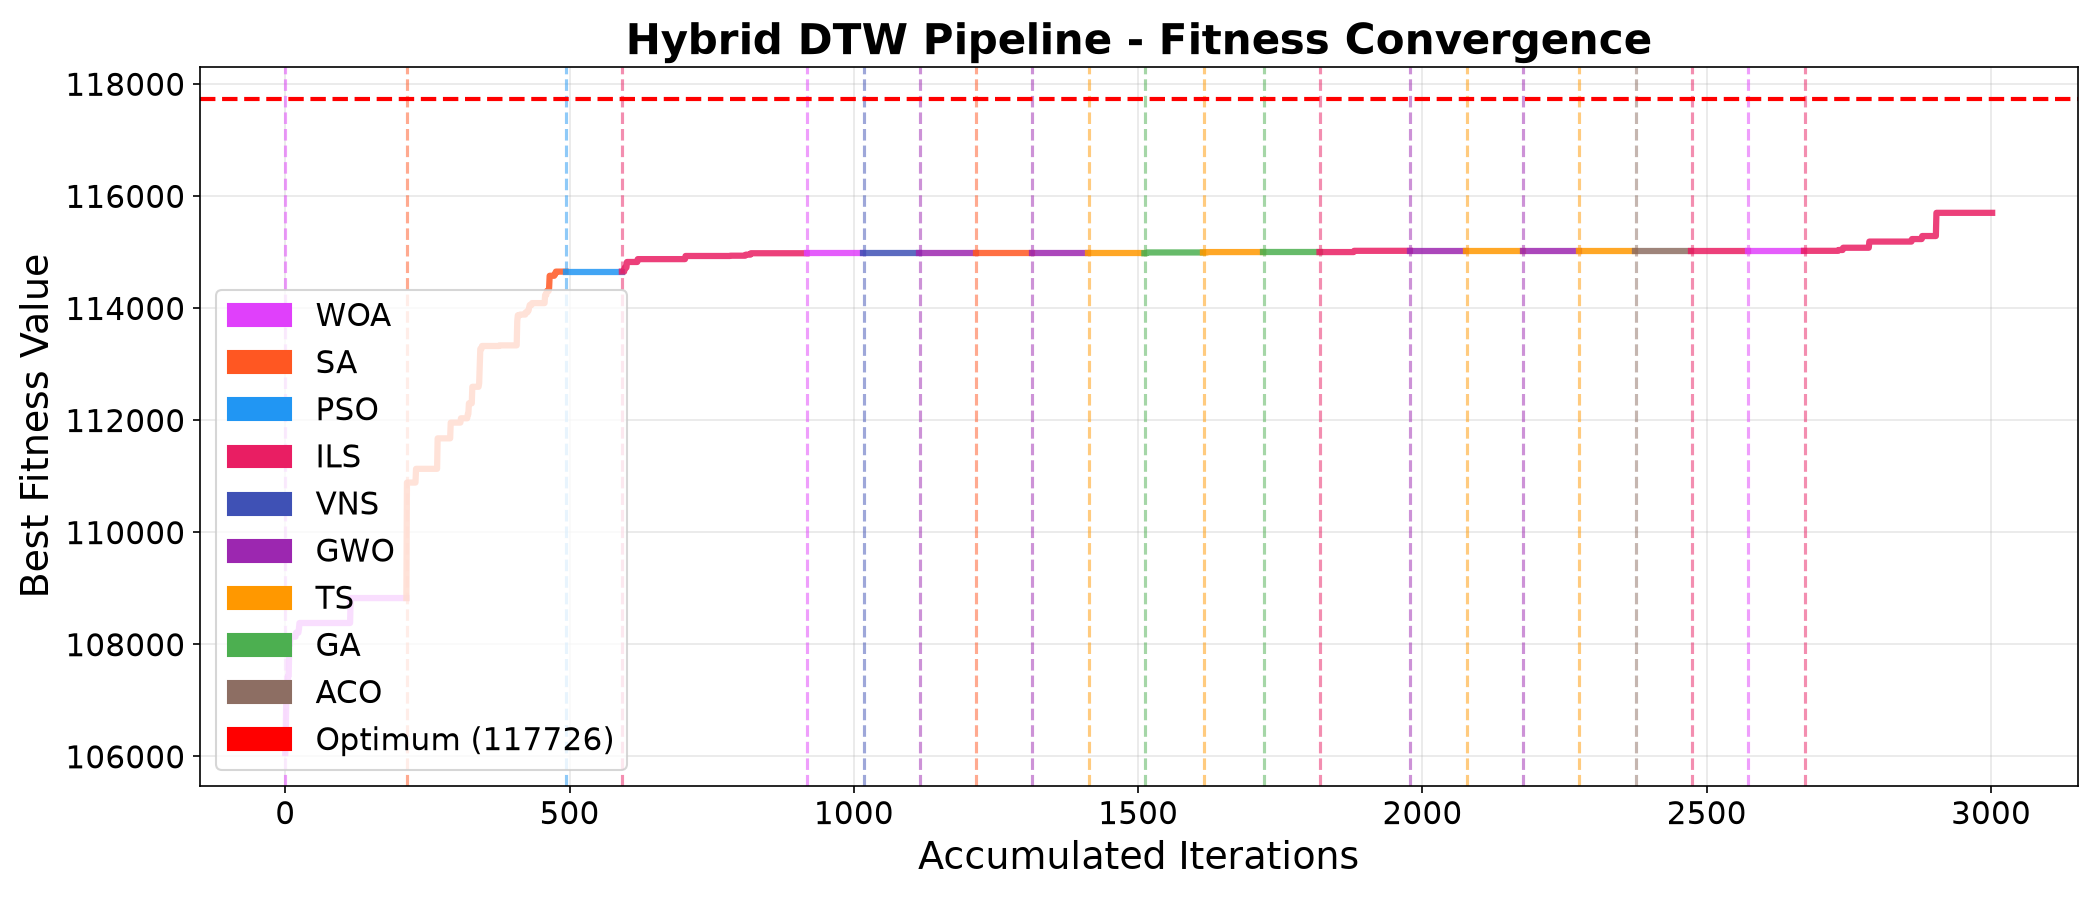
\includegraphics[width=0.32\textwidth]{imagenes_paper/mkp_dtw_3k_mknapcb6_convergencia.png}}\hfill
\subfloat[Elastic metric $\Delta=D_1-D_2$.]{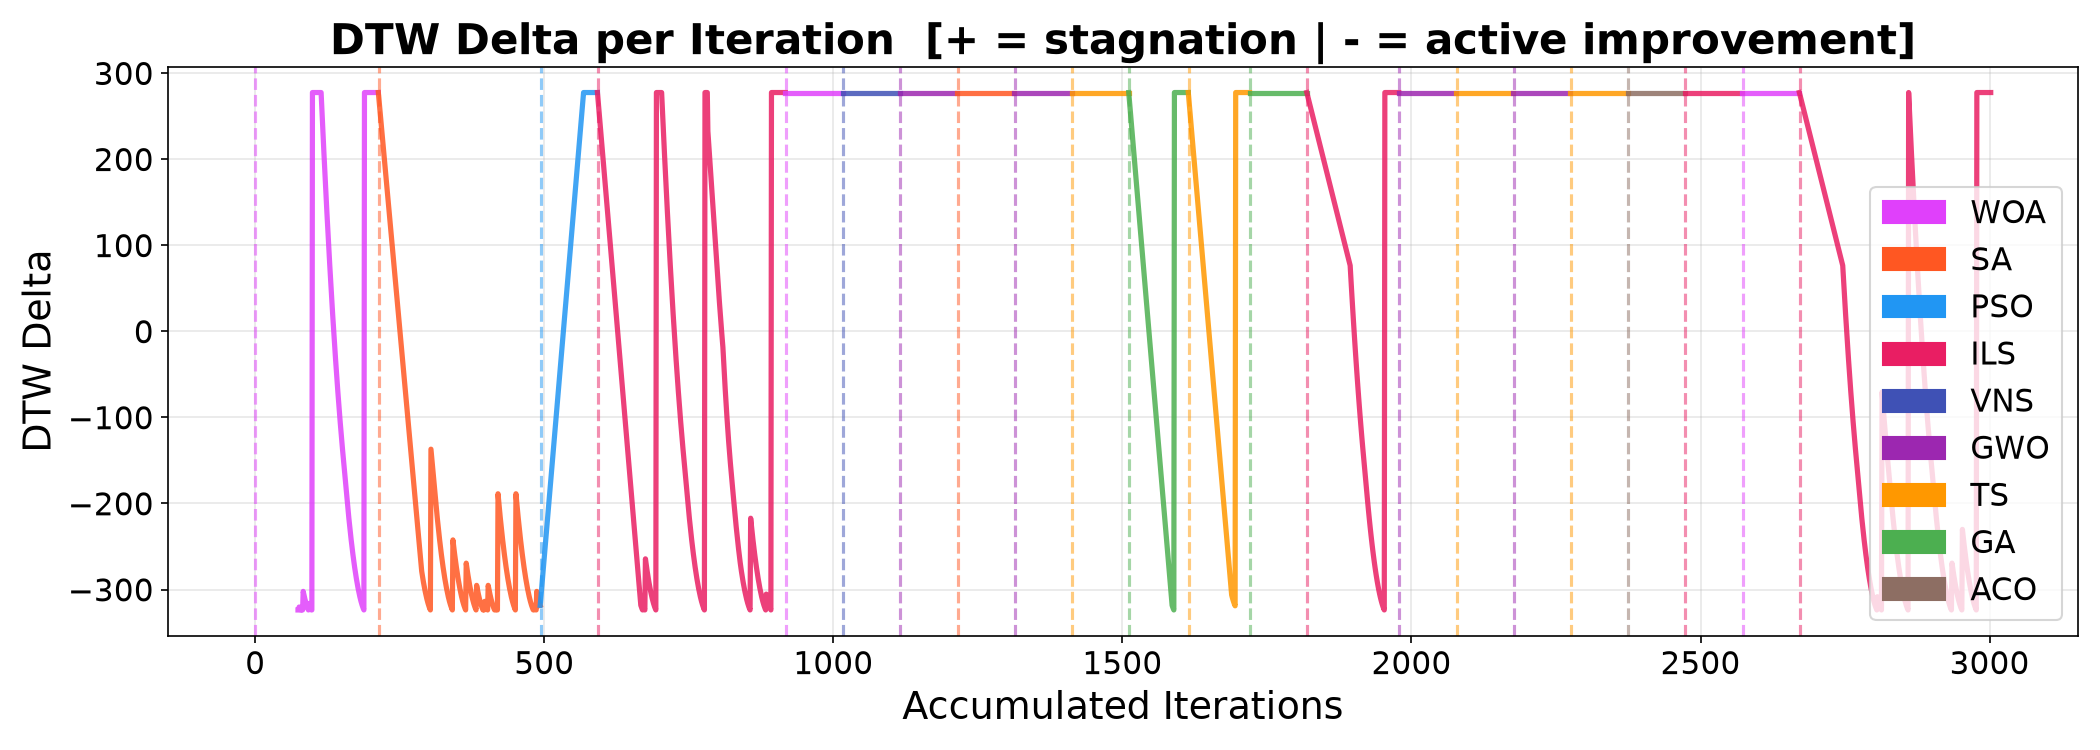
\includegraphics[width=0.32\textwidth]{imagenes_paper/mkp_dtw_3k_mknapcb6_delta.png}}
\caption{Diagnostic suite for instance \textbf{mknapcb6} ($n=500$, $m=10$) under the DTW framework with $T_{\max}=3{,}000$: (a)~final-fitness distribution over $N=31$ runs; (b)~convergence trajectory of the best run; (c)~elastic warping profile $\Delta$.}
\label{fig:mkp-best-cb6}
\end{figure}

% --- mknapcb7: DTW, 3,000 iterations ---
\begin{figure}[htbp]
\centering
\subfloat[Metaheuristic comparison.]{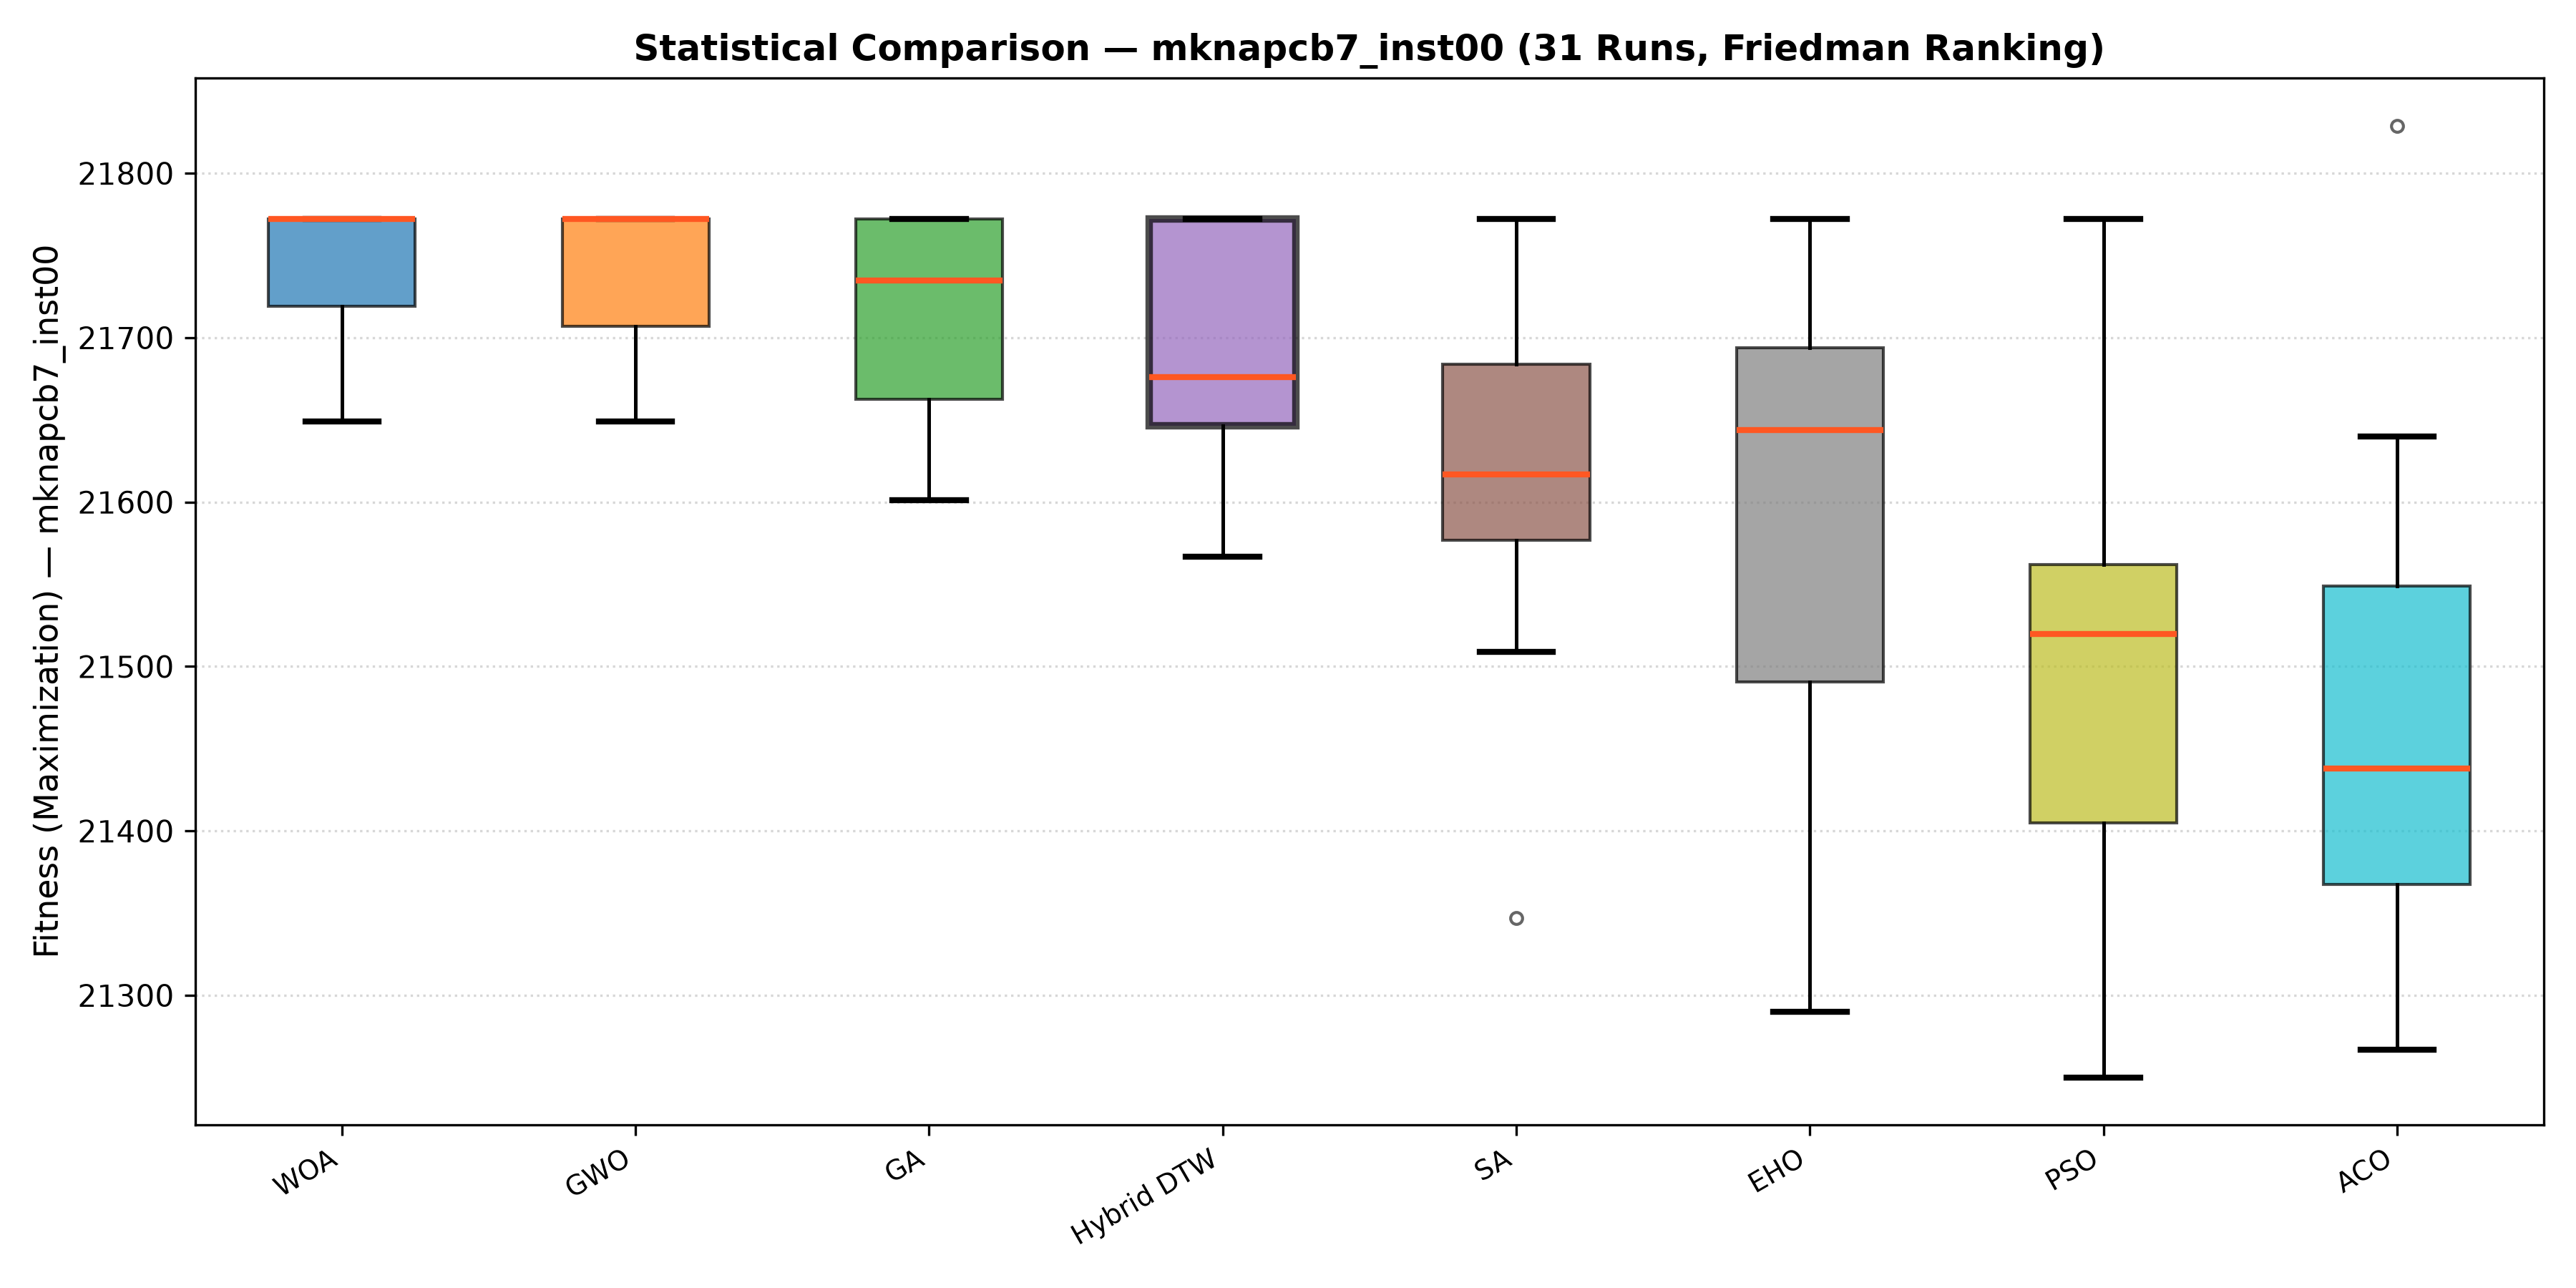
\includegraphics[width=0.32\textwidth]{imagenes_paper/mkp_dtw_3k_mknapcb7_comparativo_mh.png}}\hfill
\subfloat[Best-run convergence.]{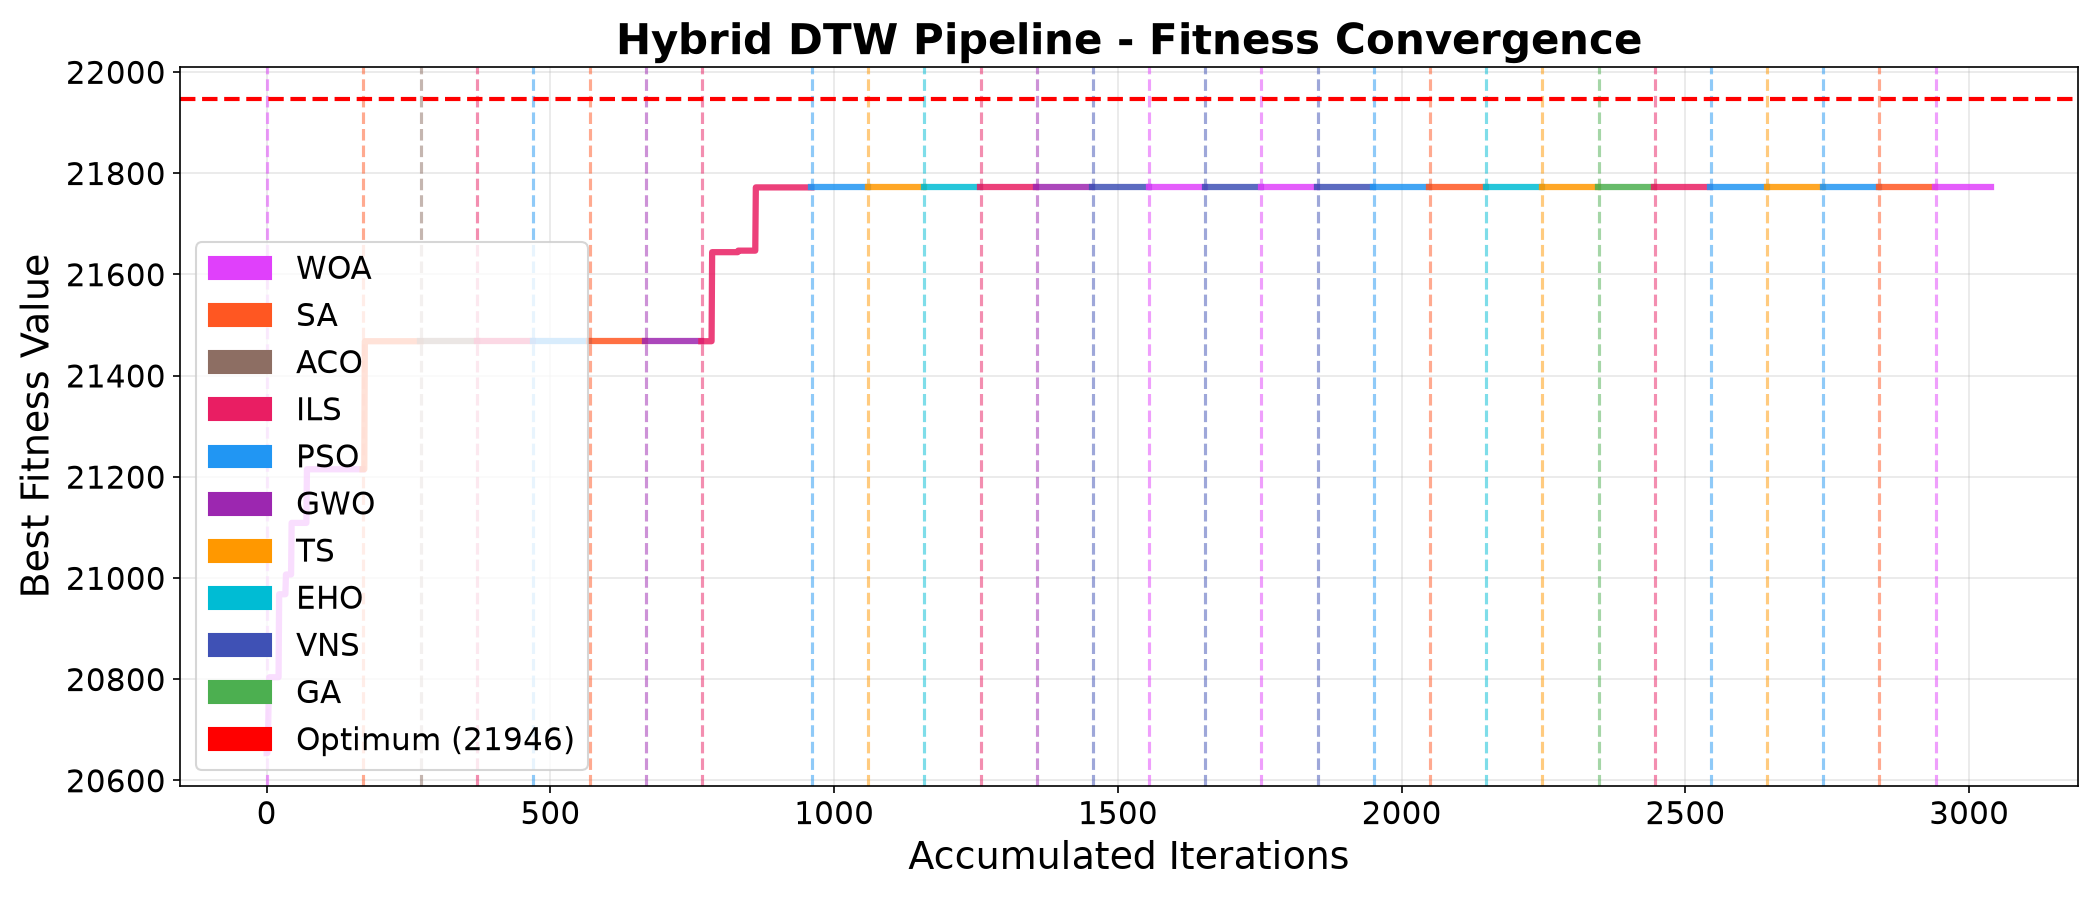
\includegraphics[width=0.32\textwidth]{imagenes_paper/mkp_dtw_3k_mknapcb7_convergencia.png}}\hfill
\subfloat[Elastic metric $\Delta=D_1-D_2$.]{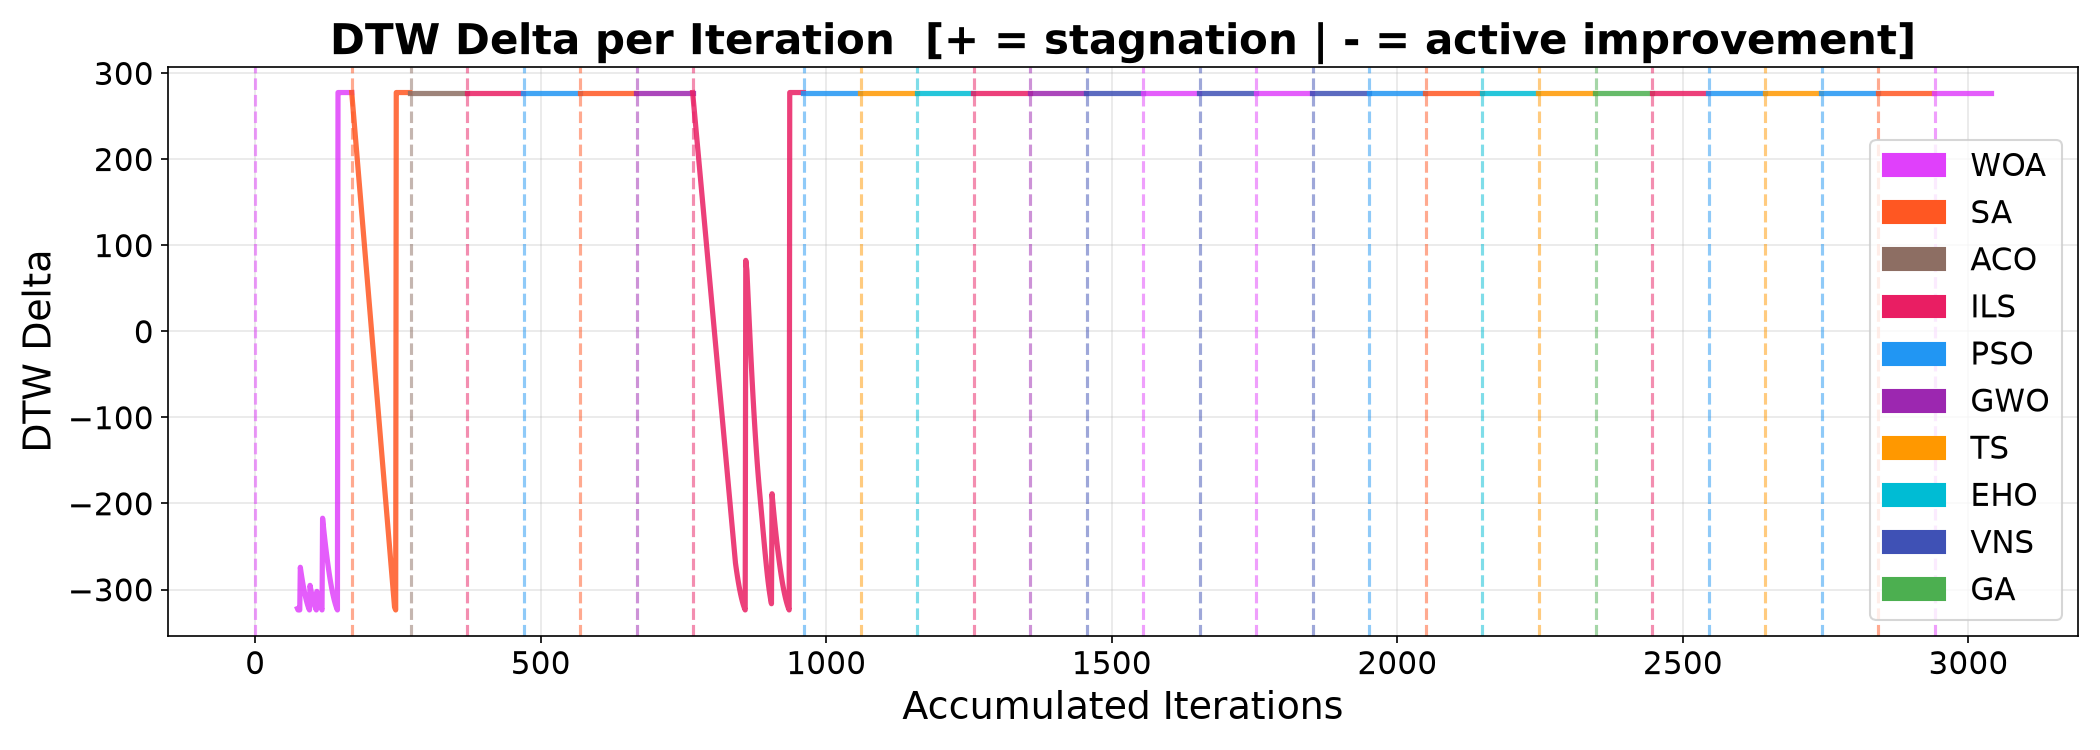
\includegraphics[width=0.32\textwidth]{imagenes_paper/mkp_dtw_3k_mknapcb7_delta.png}}
\caption{Diagnostic suite for instance \textbf{mknapcb7} ($n=100$, $m=30$) under the DTW framework with $T_{\max}=3{,}000$: (a)~final-fitness distribution over $N=31$ runs; (b)~convergence trajectory of the best run; (c)~elastic warping profile $\Delta$.}
\label{fig:mkp-best-cb7}
\end{figure}

% --- mknapcb8: DTW, 3,000 iterations ---
\begin{figure}[htbp]
\centering
\subfloat[Metaheuristic comparison.]{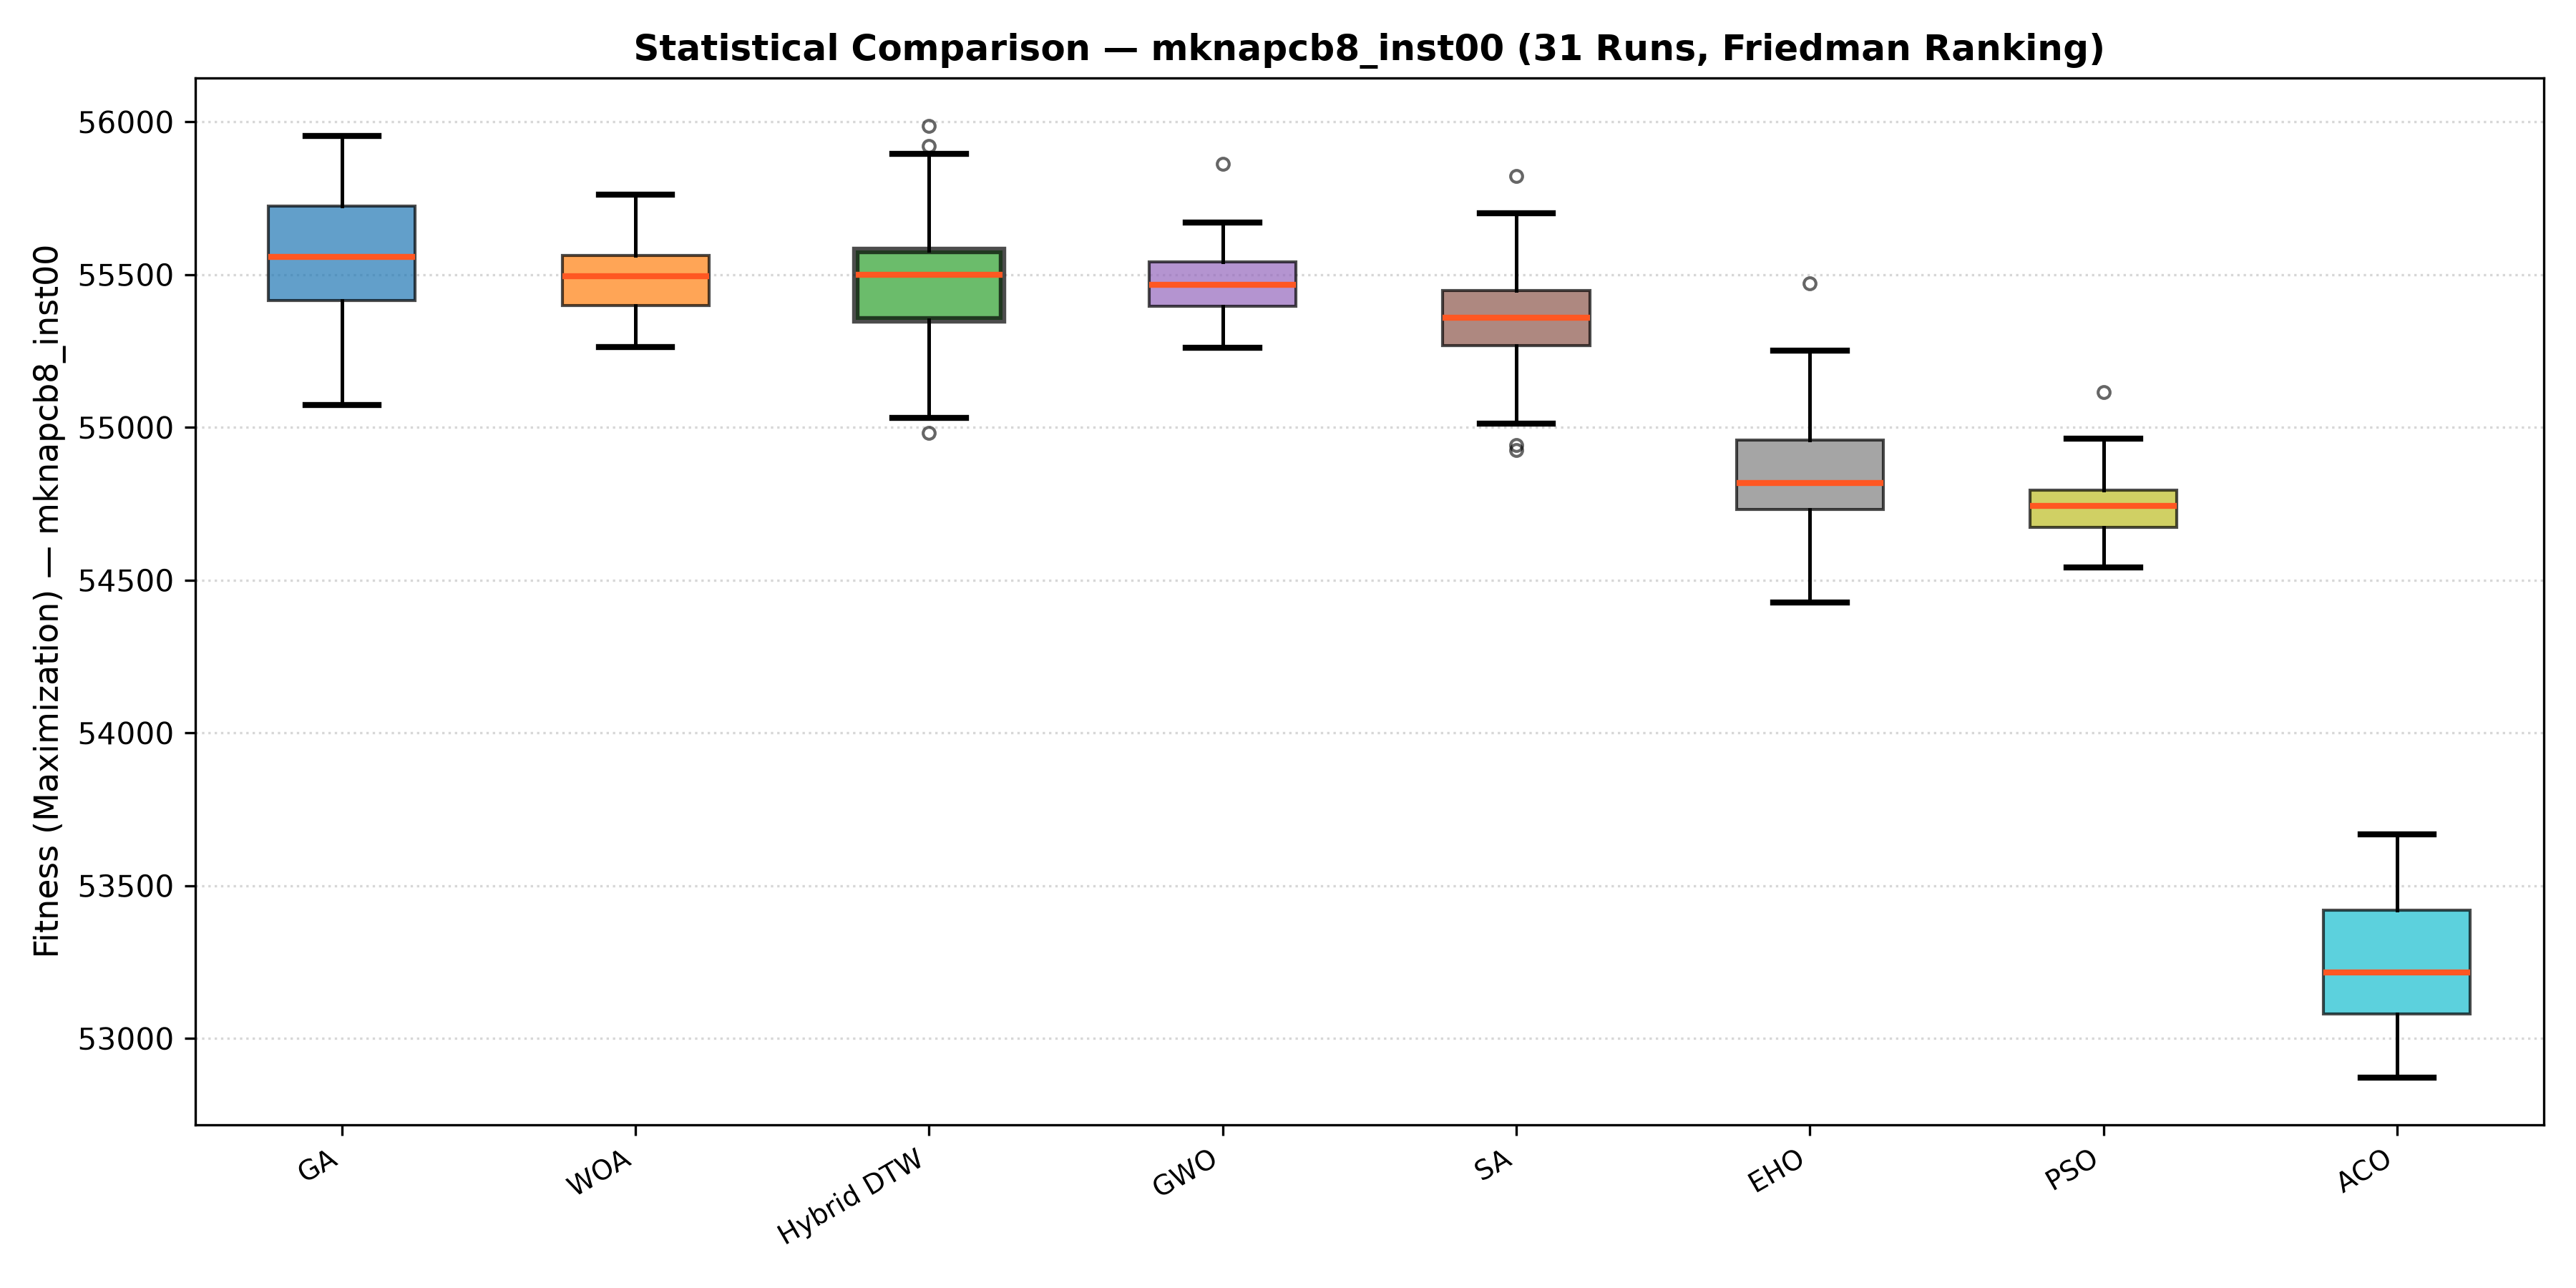
\includegraphics[width=0.32\textwidth]{imagenes_paper/mkp_dtw_3k_mknapcb8_comparativo_mh.png}}\hfill
\subfloat[Best-run convergence.]{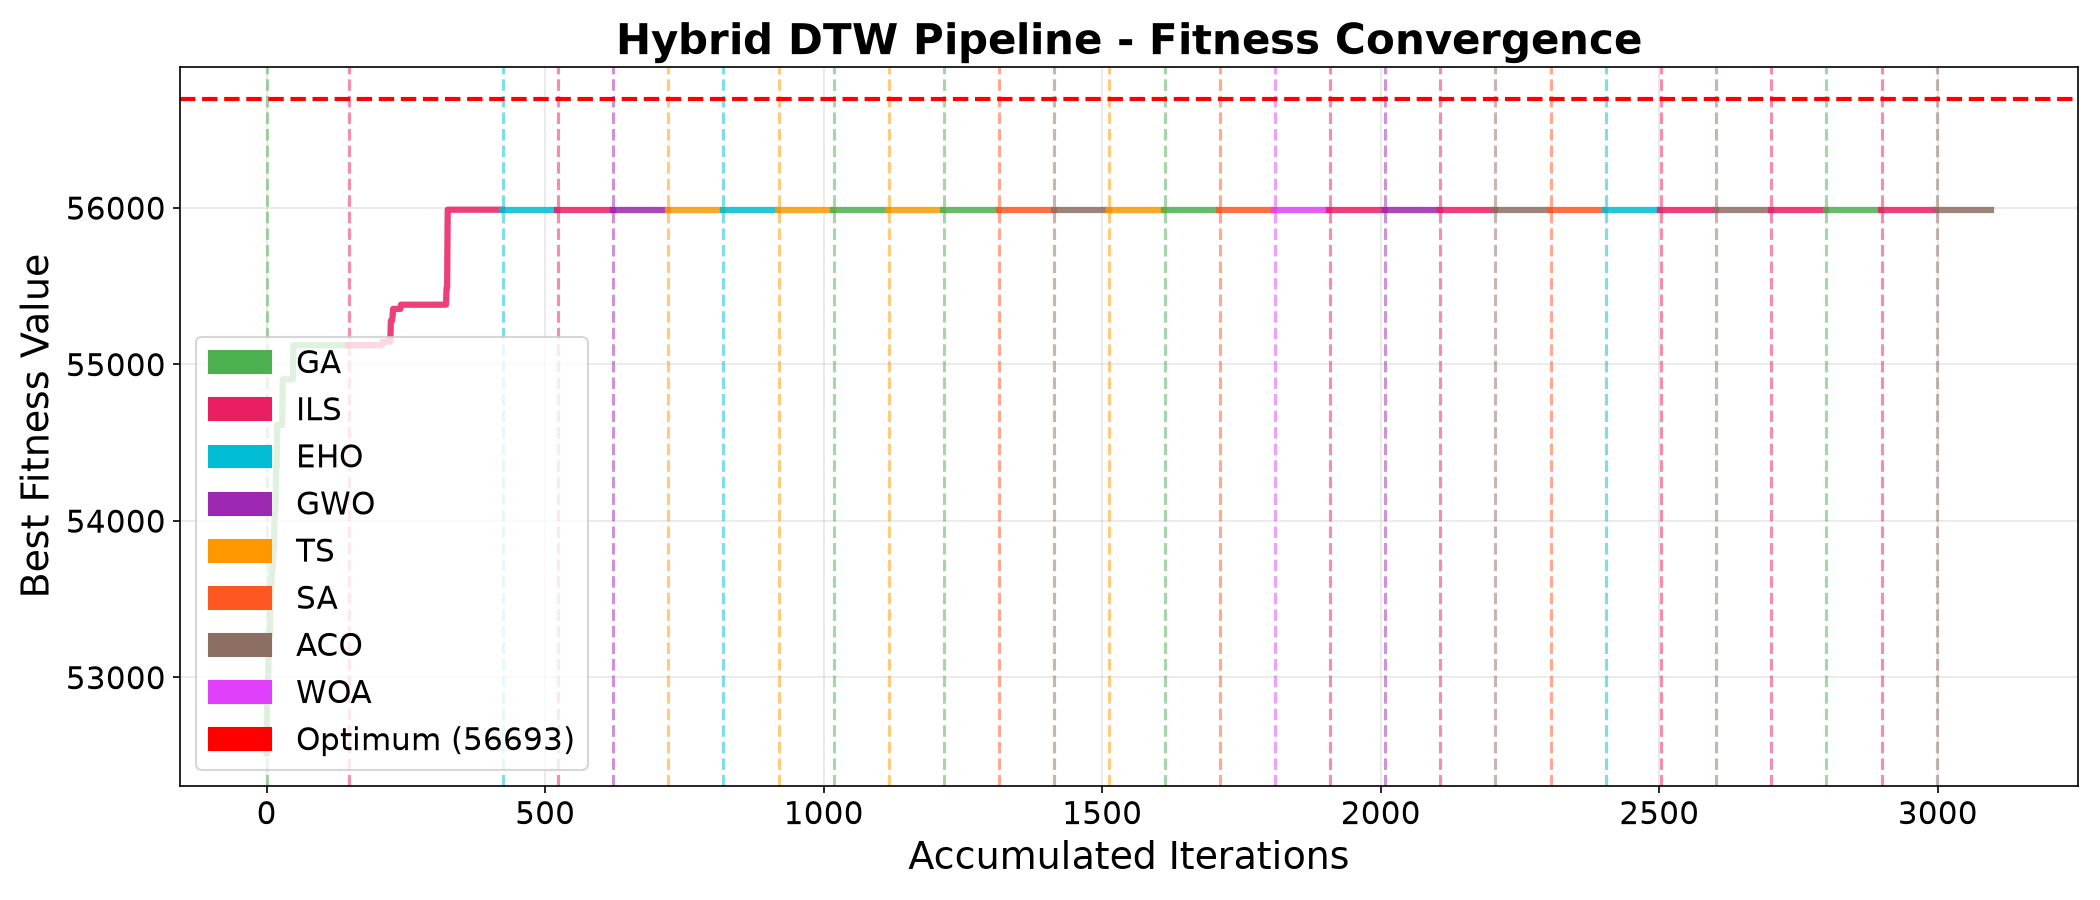
\includegraphics[width=0.32\textwidth]{imagenes_paper/mkp_dtw_3k_mknapcb8_convergencia.png}}\hfill
\subfloat[Elastic metric $\Delta=D_1-D_2$.]{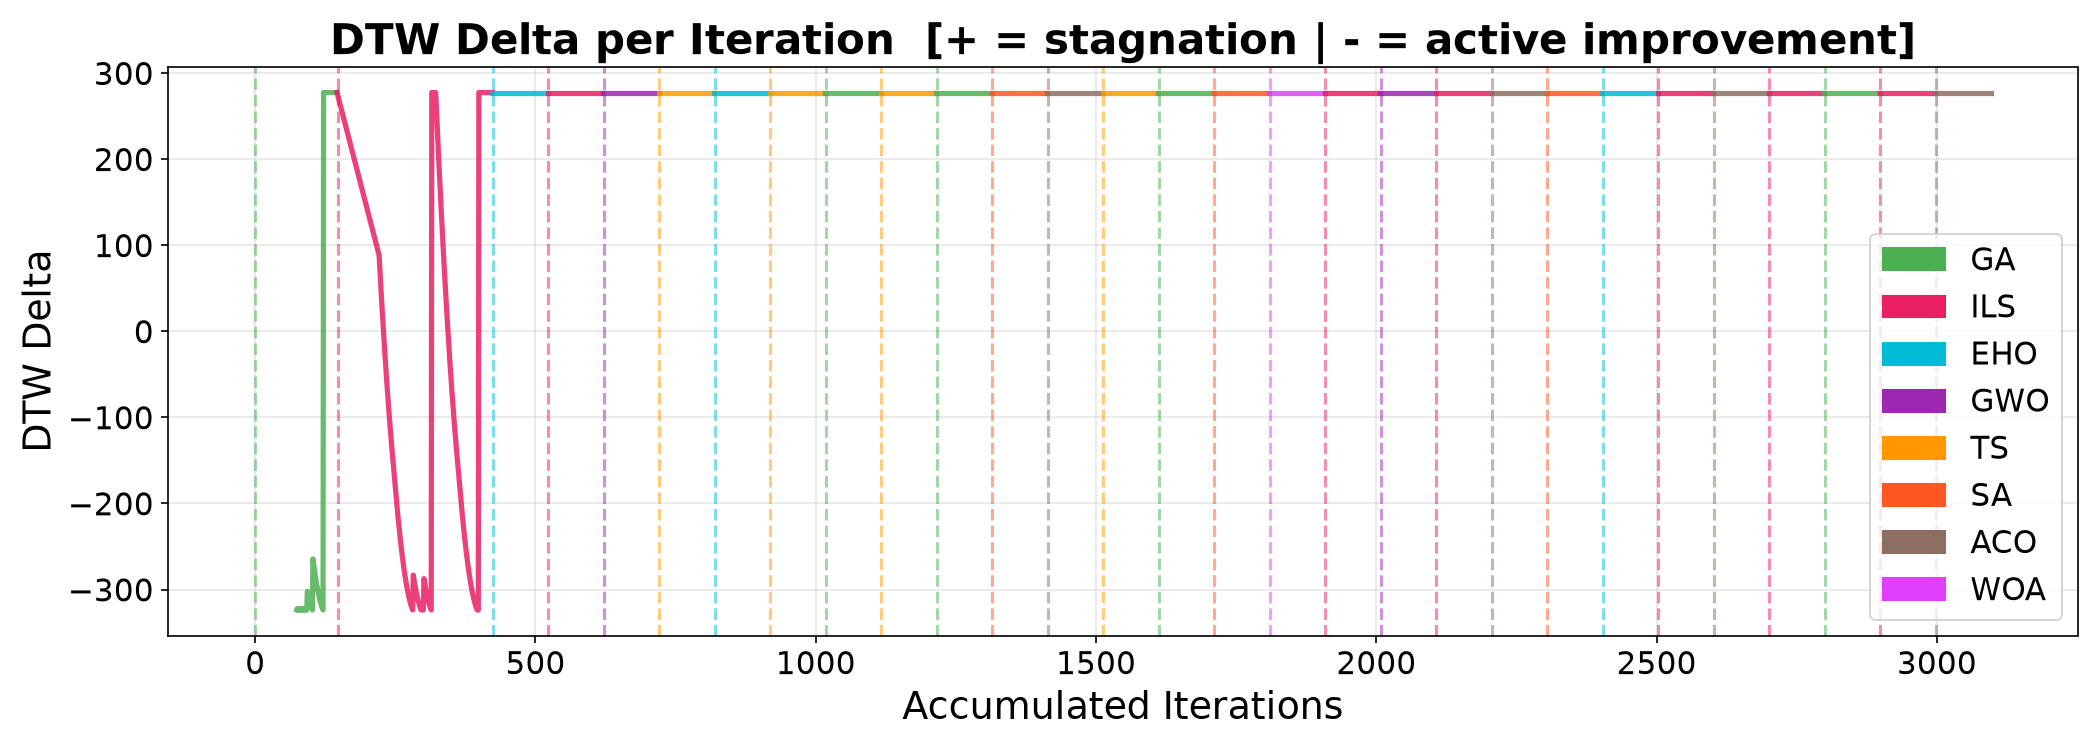
\includegraphics[width=0.32\textwidth]{imagenes_paper/mkp_dtw_3k_mknapcb8_delta.png}}
\caption{Diagnostic suite for instance \textbf{mknapcb8} ($n=250$, $m=30$) under the DTW framework with $T_{\max}=3{,}000$: (a)~final-fitness distribution over $N=31$ runs; (b)~convergence trajectory of the best run; (c)~elastic warping profile $\Delta$.}
\label{fig:mkp-best-cb8}
\end{figure}

% --- mknapcb9: DDTW, 3,000 iterations ---
\begin{figure}[htbp]
\centering
\subfloat[Metaheuristic comparison.]{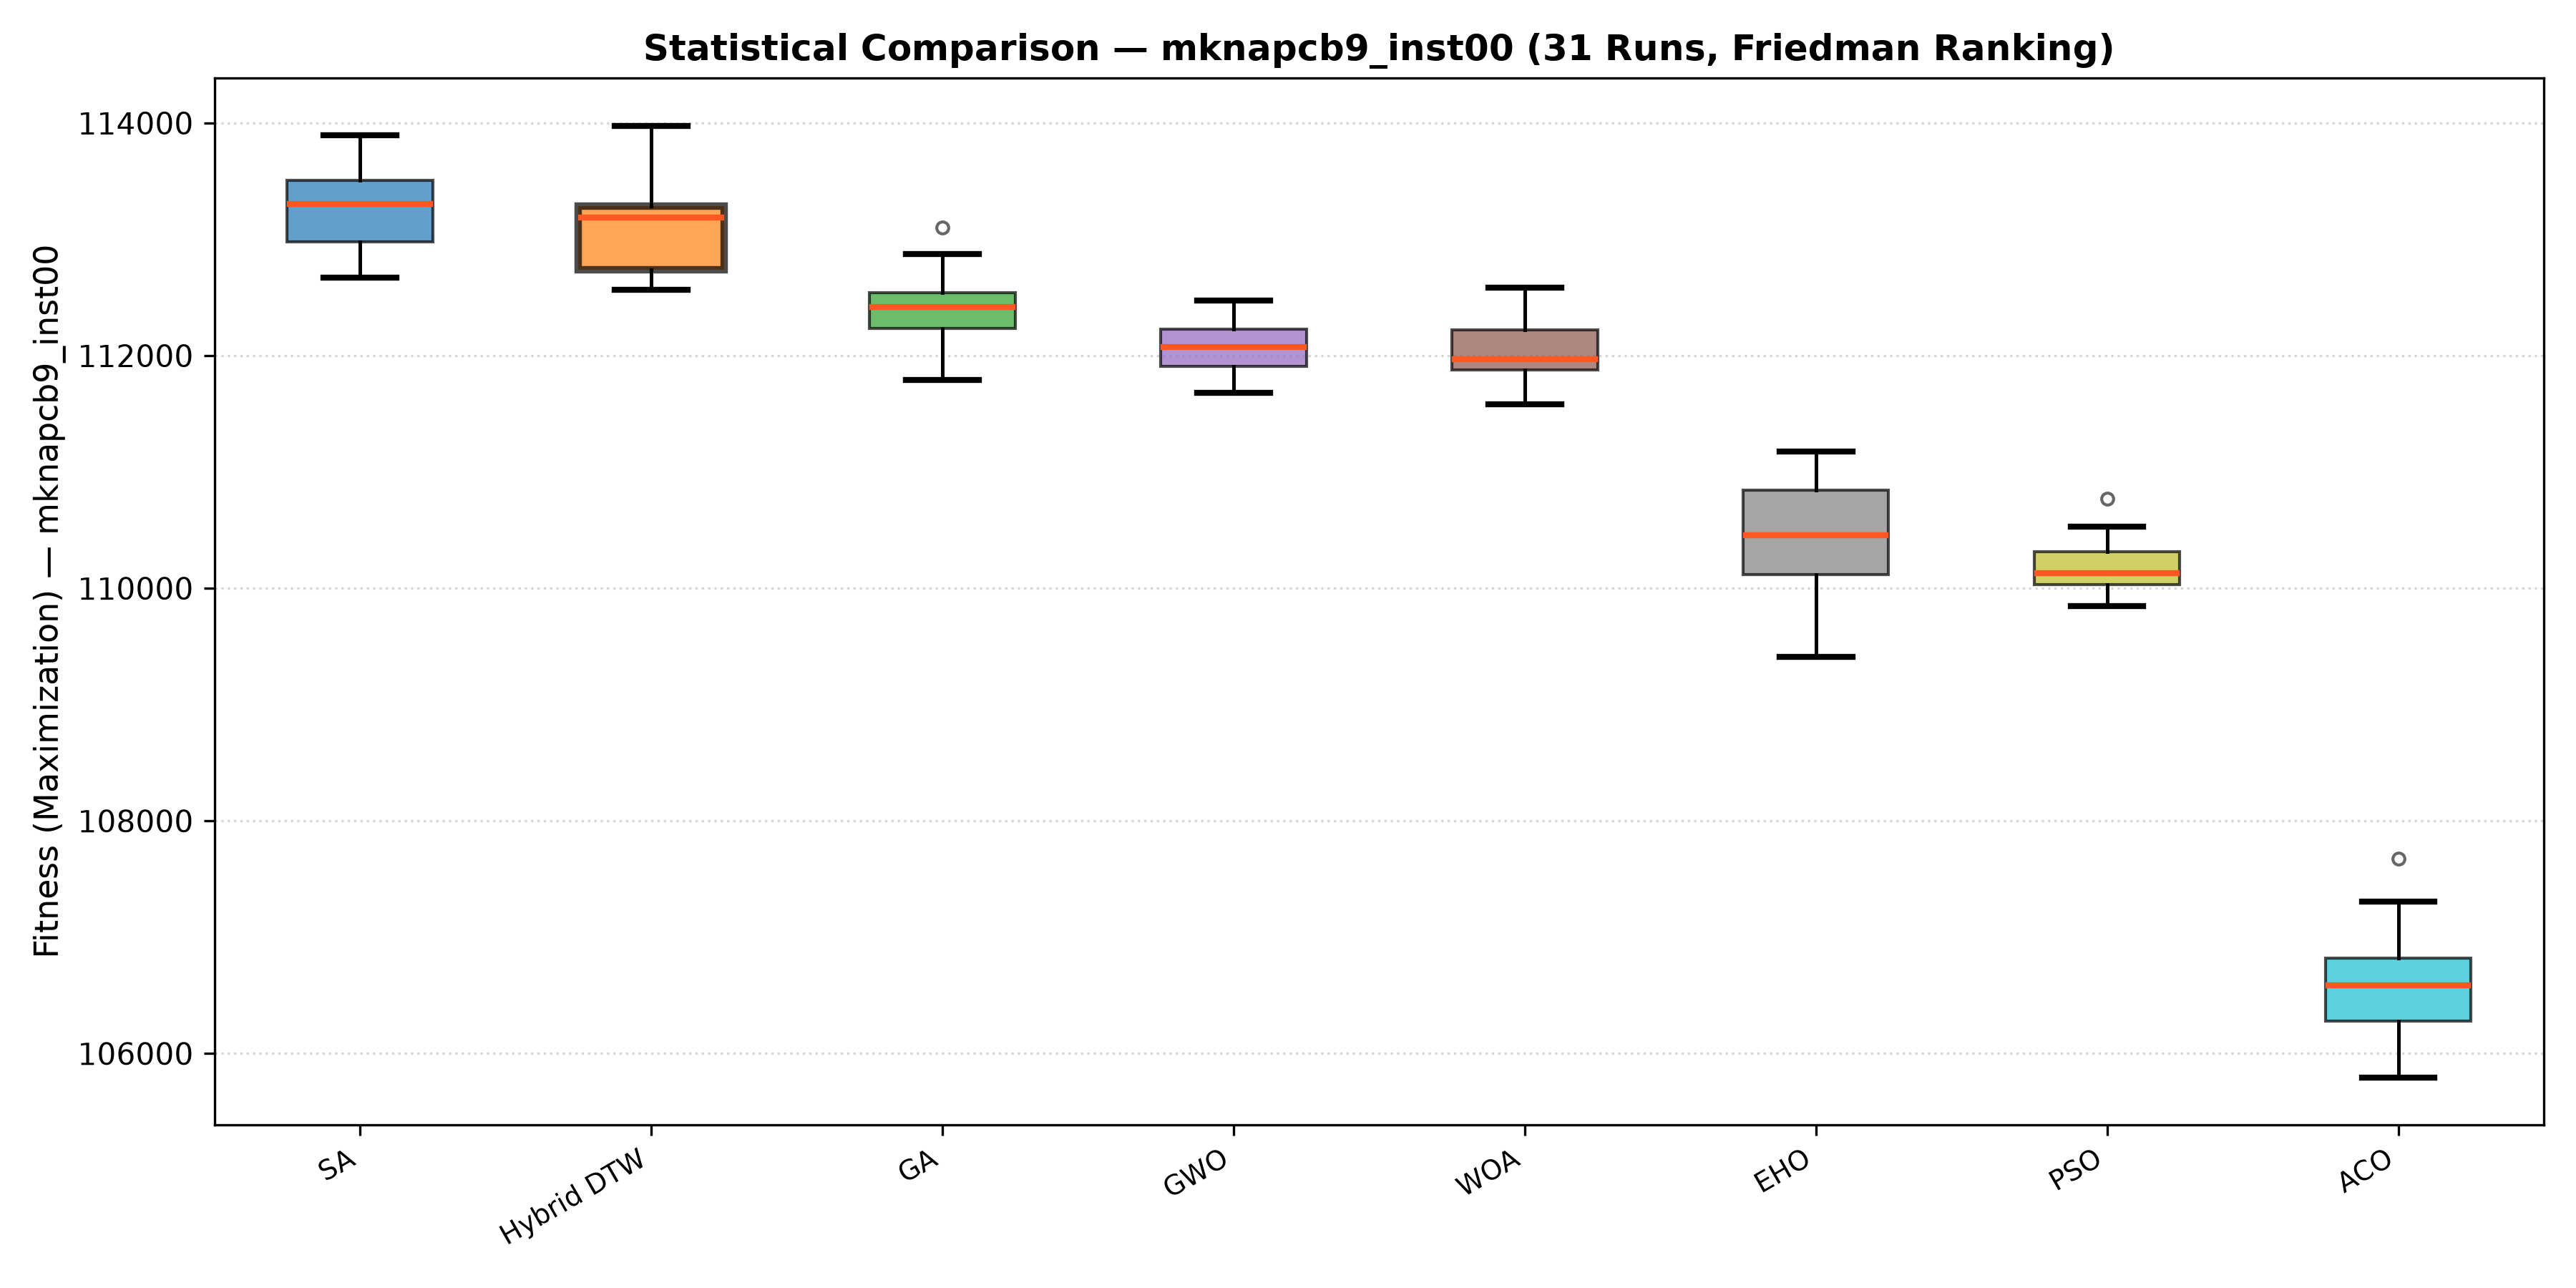
\includegraphics[width=0.32\textwidth]{imagenes_paper/mkp_ddtw_3k_mknapcb9_comparativo_mh.png}}\hfill
\subfloat[Best-run convergence.]{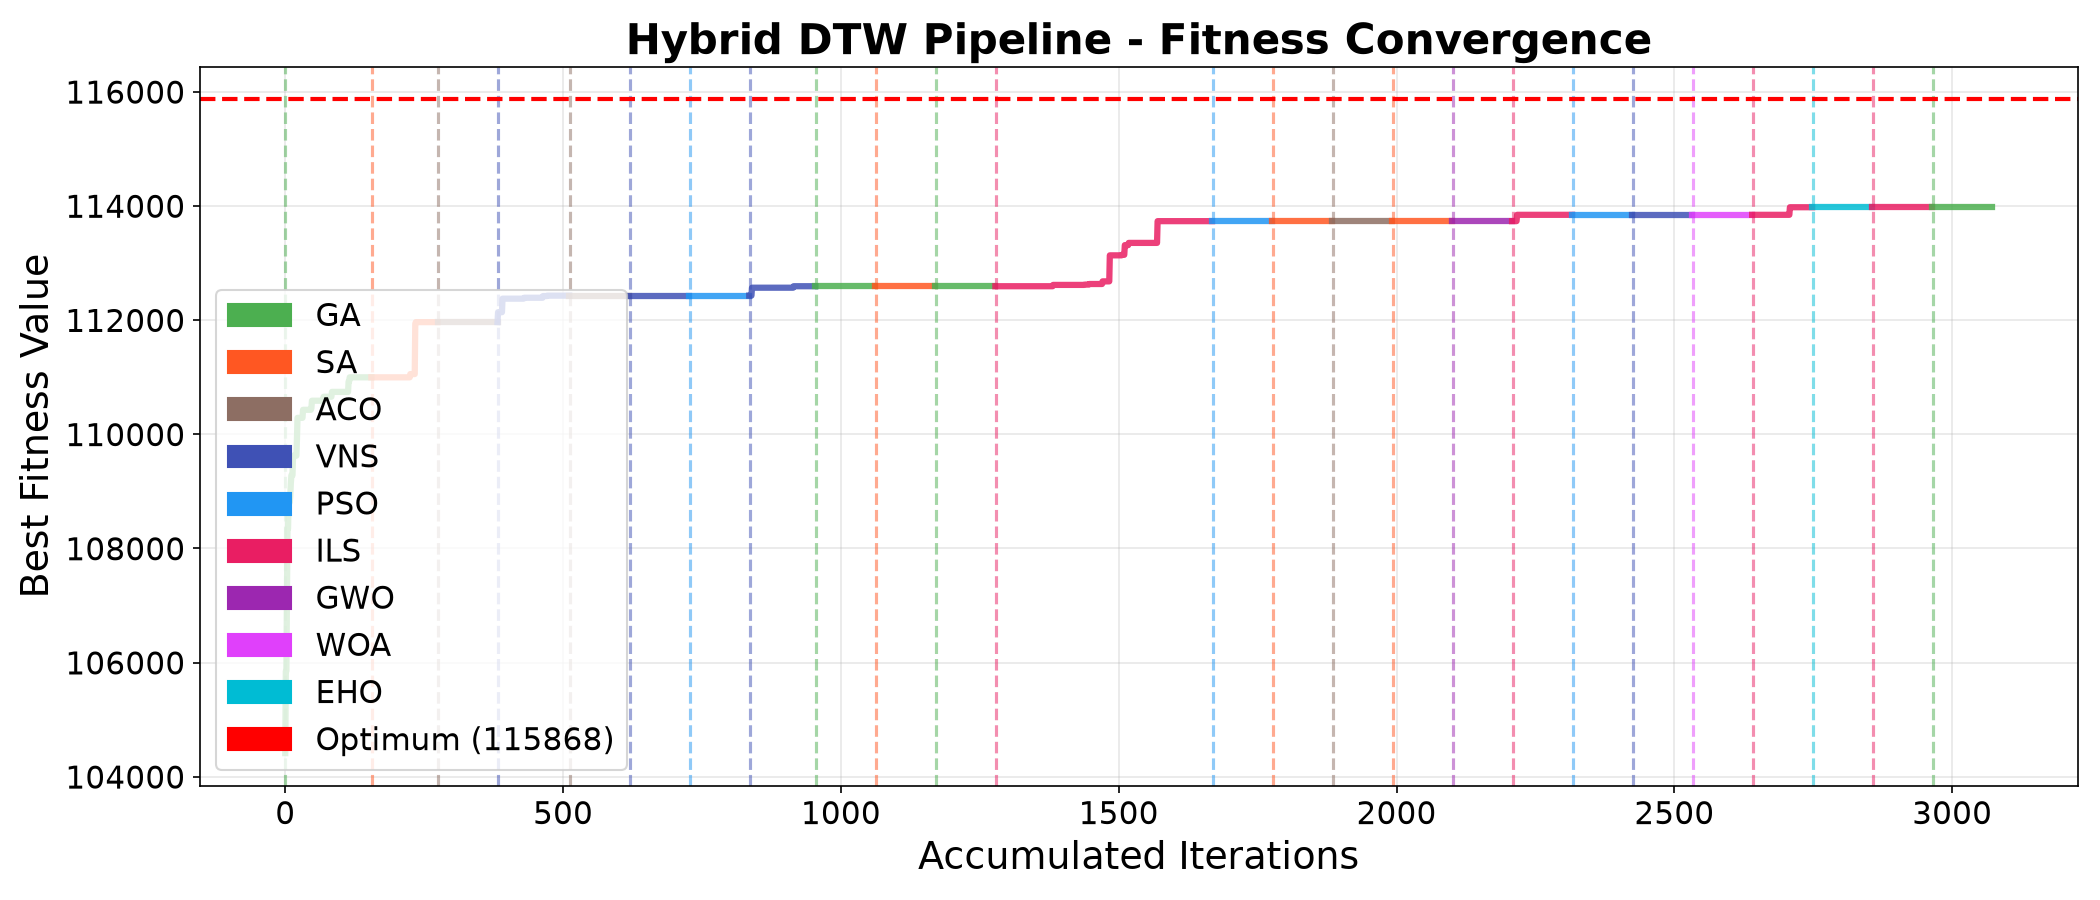
\includegraphics[width=0.32\textwidth]{imagenes_paper/mkp_ddtw_3k_mknapcb9_convergencia.png}}\hfill
\subfloat[Elastic metric $\Delta=D_1-D_2$.]{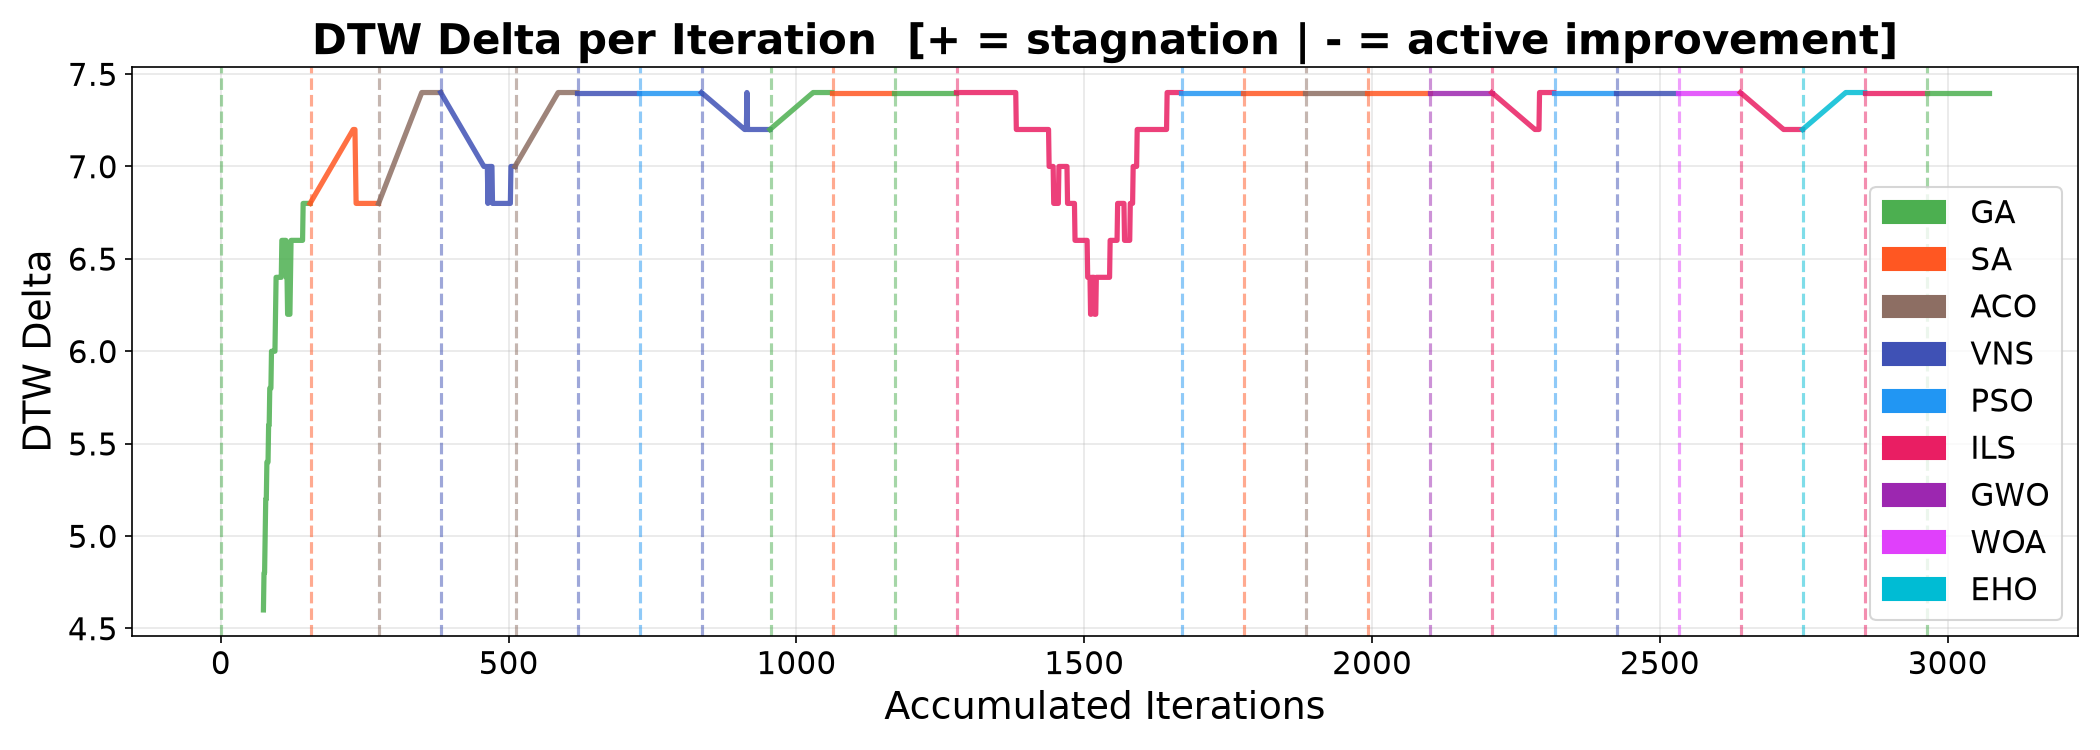
\includegraphics[width=0.32\textwidth]{imagenes_paper/mkp_ddtw_3k_mknapcb9_delta.png}}
\caption{Diagnostic suite for instance \textbf{mknapcb9} ($n=500$, $m=30$) under the DDTW framework with $T_{\max}=3{,}000$: (a)~final-fitness distribution over $N=31$ runs; (b)~convergence trajectory of the best run; (c)~elastic warping profile $\Delta$.}
\label{fig:mkp-best-cb9}
\end{figure}

% Required packages: graphicx, subfig (or subcaption with \subfloat redefined).

% Each figure shows the best-performing framework configuration for the
% corresponding instance, selected by highest mean fitness over 31 runs.
% DTW--3K is best for mknapcb1 and mknapcb3--mknapcb8;
% DDTW--3K is best for mknapcb2 and mknapcb9.

Figures~\ref{fig:mkp-best-cb1}--\ref{fig:mkp-best-cb9} present the
diagnostic suite for each of the nine Chu--Beasley MKP instances under its
best-performing framework configuration, selected by highest mean fitness
over the 31 runs, with corresponding executions treated as paired. DTW with $T_{\max}=3{,}000$ achieved the
highest mean in seven instances (mknapcb1 and mknapcb3--mknapcb8), while
DDTW with $T_{\max}=3{,}000$ was superior for mknapcb2 and mknapcb9.
Each figure comprises three panels: (a)~a box-plot comparing the
final-fitness distributions of the hybrid framework against the standalone
metaheuristics over the 31 runs, allowing visual assessment of both central
tendency and dispersion; (b)~the convergence trajectory of the best run,
showing the evolution of the incumbent fitness along with the solver
transitions triggered by the stagnation monitor; and (c)~the elastic
warping profile $\Delta = D_1 - D_2$, where positive values indicate
detected stagnation phases and negative values correspond to periods of
active improvement.

% --- mknapcb1: DTW, 3,000 iterations ---
\begin{figure}[htbp]
\centering
\subfloat[Metaheuristic comparison.]{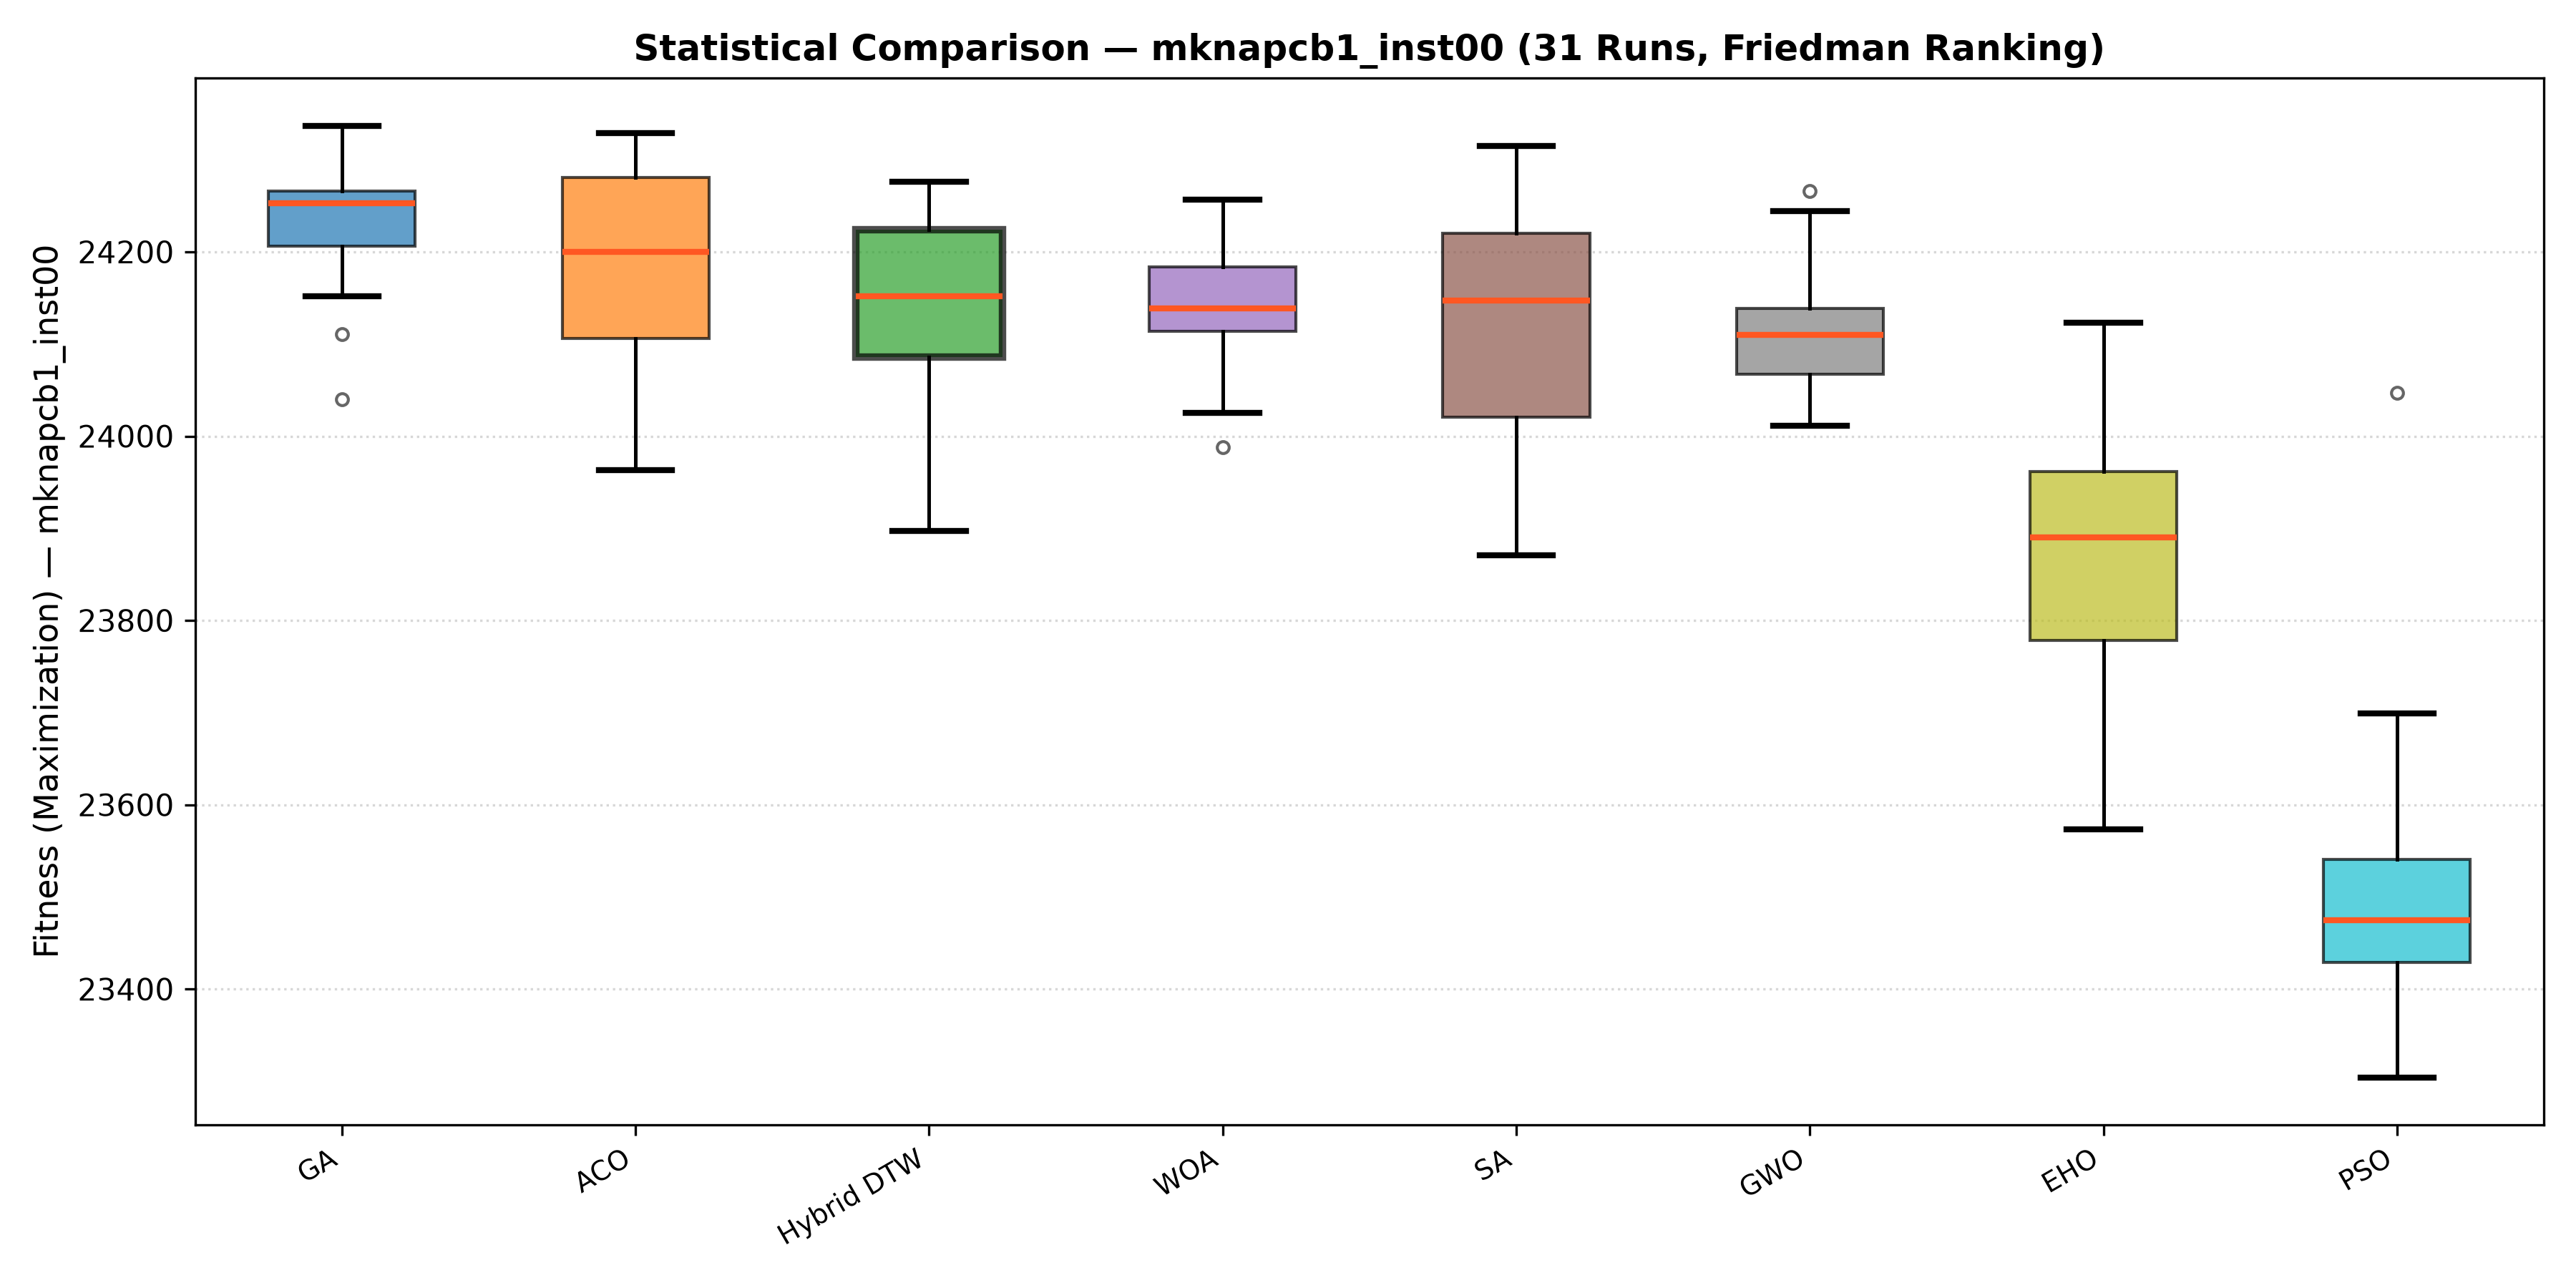
\includegraphics[width=0.32\textwidth]{imagenes_paper/mkp_dtw_3k_mknapcb1_comparativo_mh.png}}\hfill
\subfloat[Best-run convergence.]{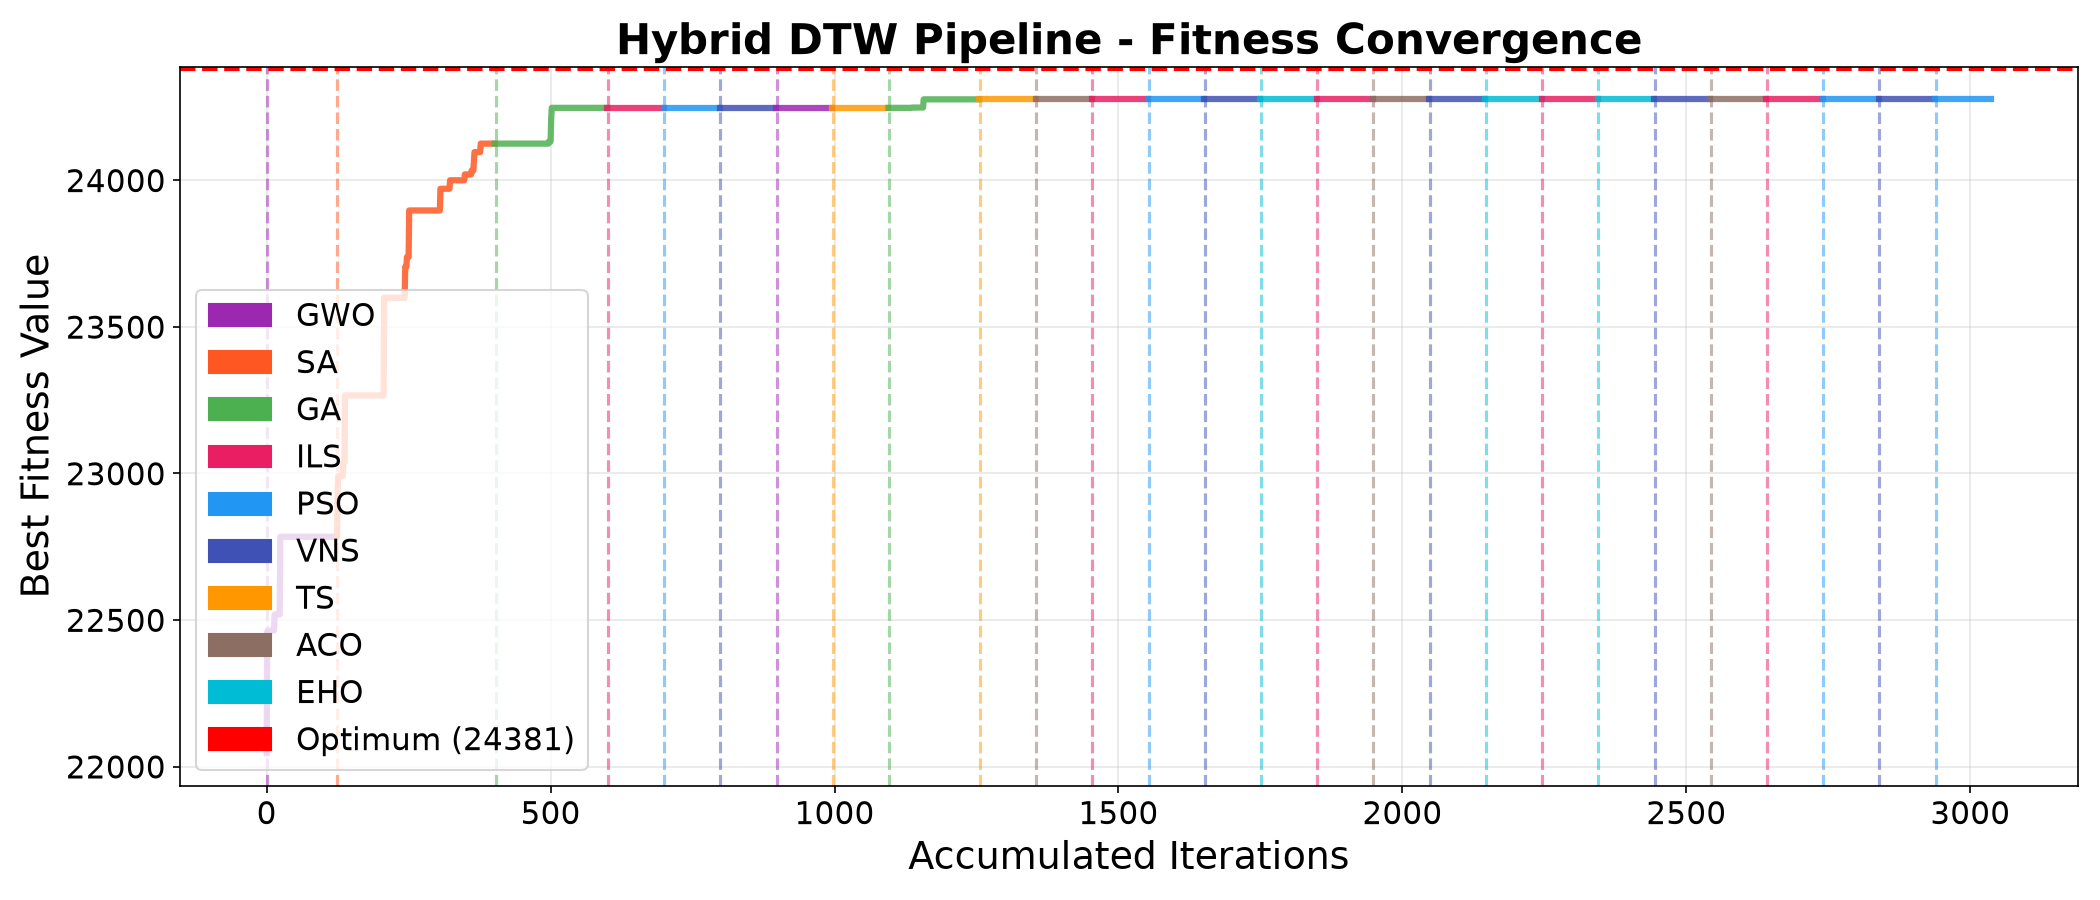
\includegraphics[width=0.32\textwidth]{imagenes_paper/mkp_dtw_3k_mknapcb1_convergencia.png}}\hfill
\subfloat[Elastic metric $\Delta=D_1-D_2$.]{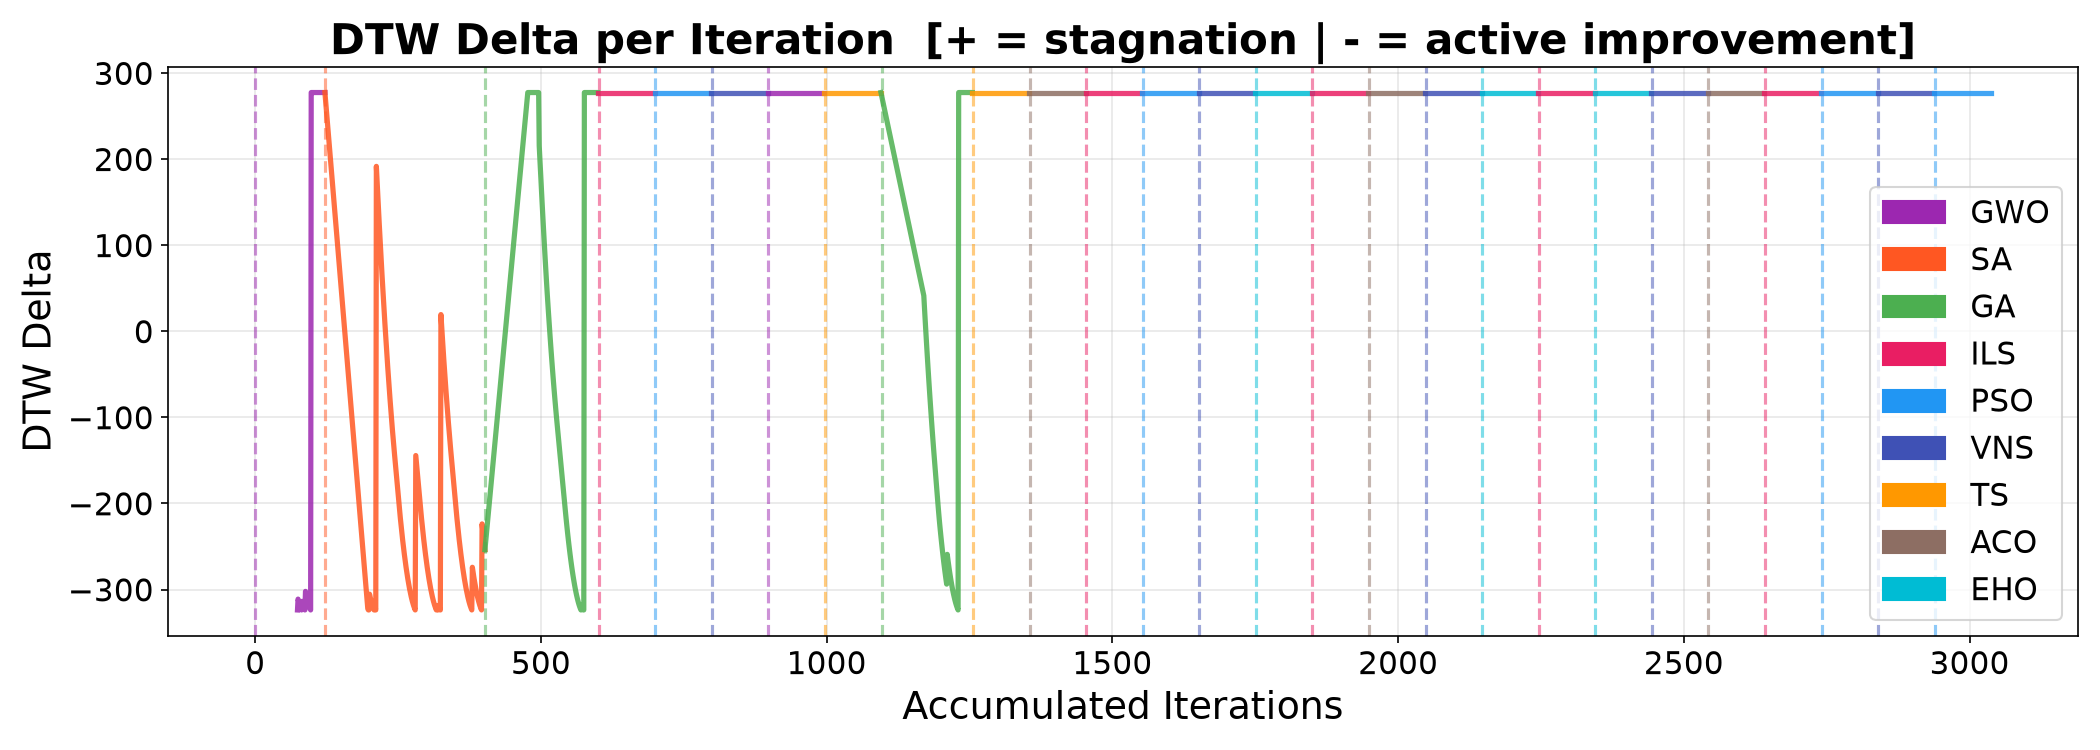
\includegraphics[width=0.32\textwidth]{imagenes_paper/mkp_dtw_3k_mknapcb1_delta.png}}
\caption{Diagnostic suite for instance \textbf{mknapcb1} ($n=100$, $m=5$) under the DTW framework with $T_{\max}=3{,}000$: (a)~final-fitness distribution over $N=31$ runs; (b)~convergence trajectory of the best run; (c)~elastic warping profile $\Delta$.}
\label{fig:mkp-best-cb1}
\end{figure}

% --- mknapcb2: DDTW, 3,000 iterations ---
\begin{figure}[htbp]
\centering
\subfloat[Metaheuristic comparison.]{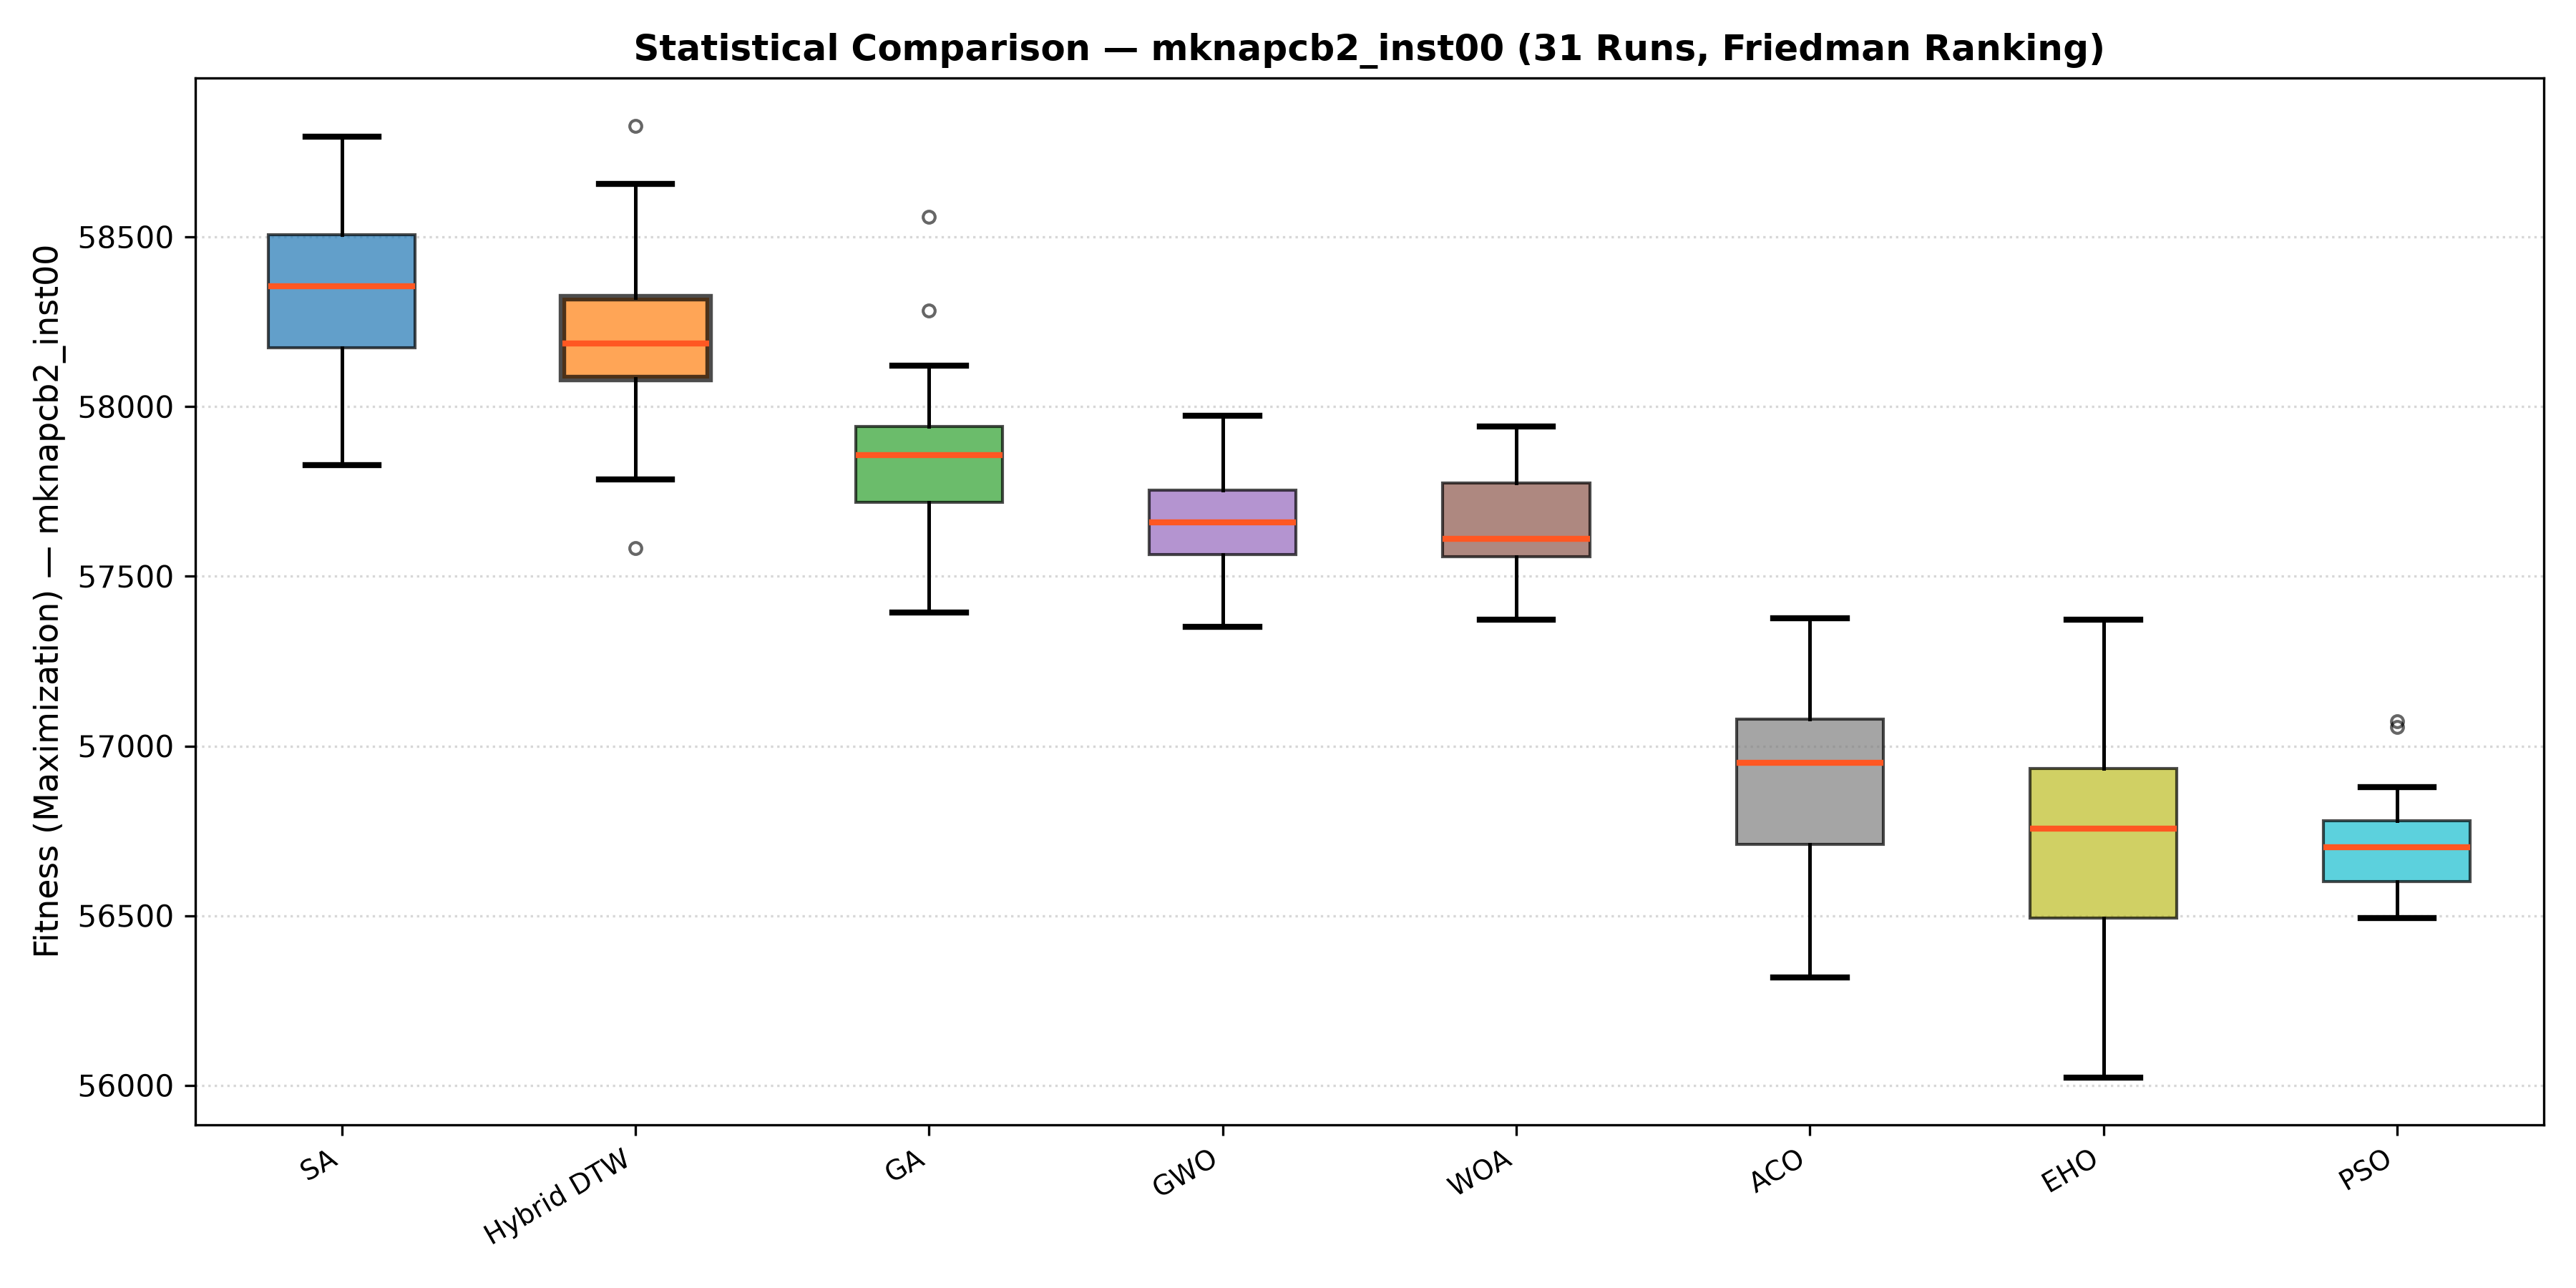
\includegraphics[width=0.32\textwidth]{imagenes_paper/mkp_ddtw_3k_mknapcb2_comparativo_mh.png}}\hfill
\subfloat[Best-run convergence.]{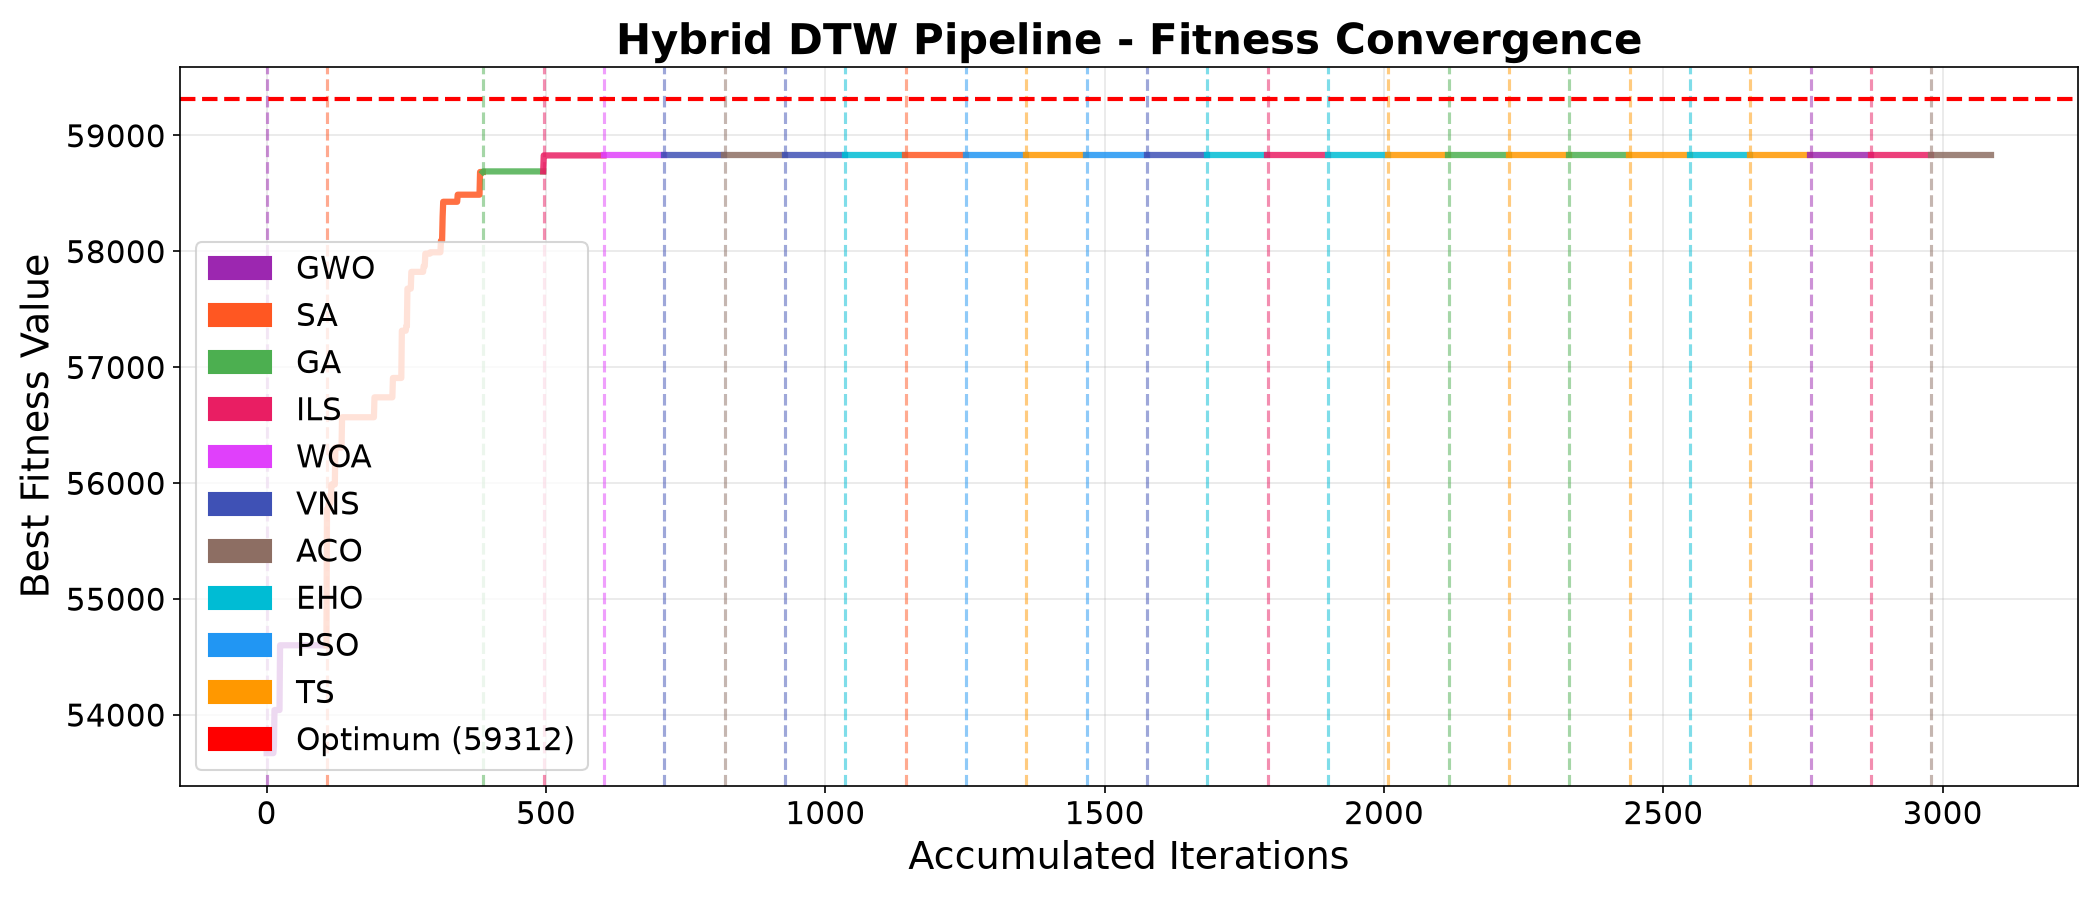
\includegraphics[width=0.32\textwidth]{imagenes_paper/mkp_ddtw_3k_mknapcb2_convergencia.png}}\hfill
\subfloat[Elastic metric $\Delta=D_1-D_2$.]{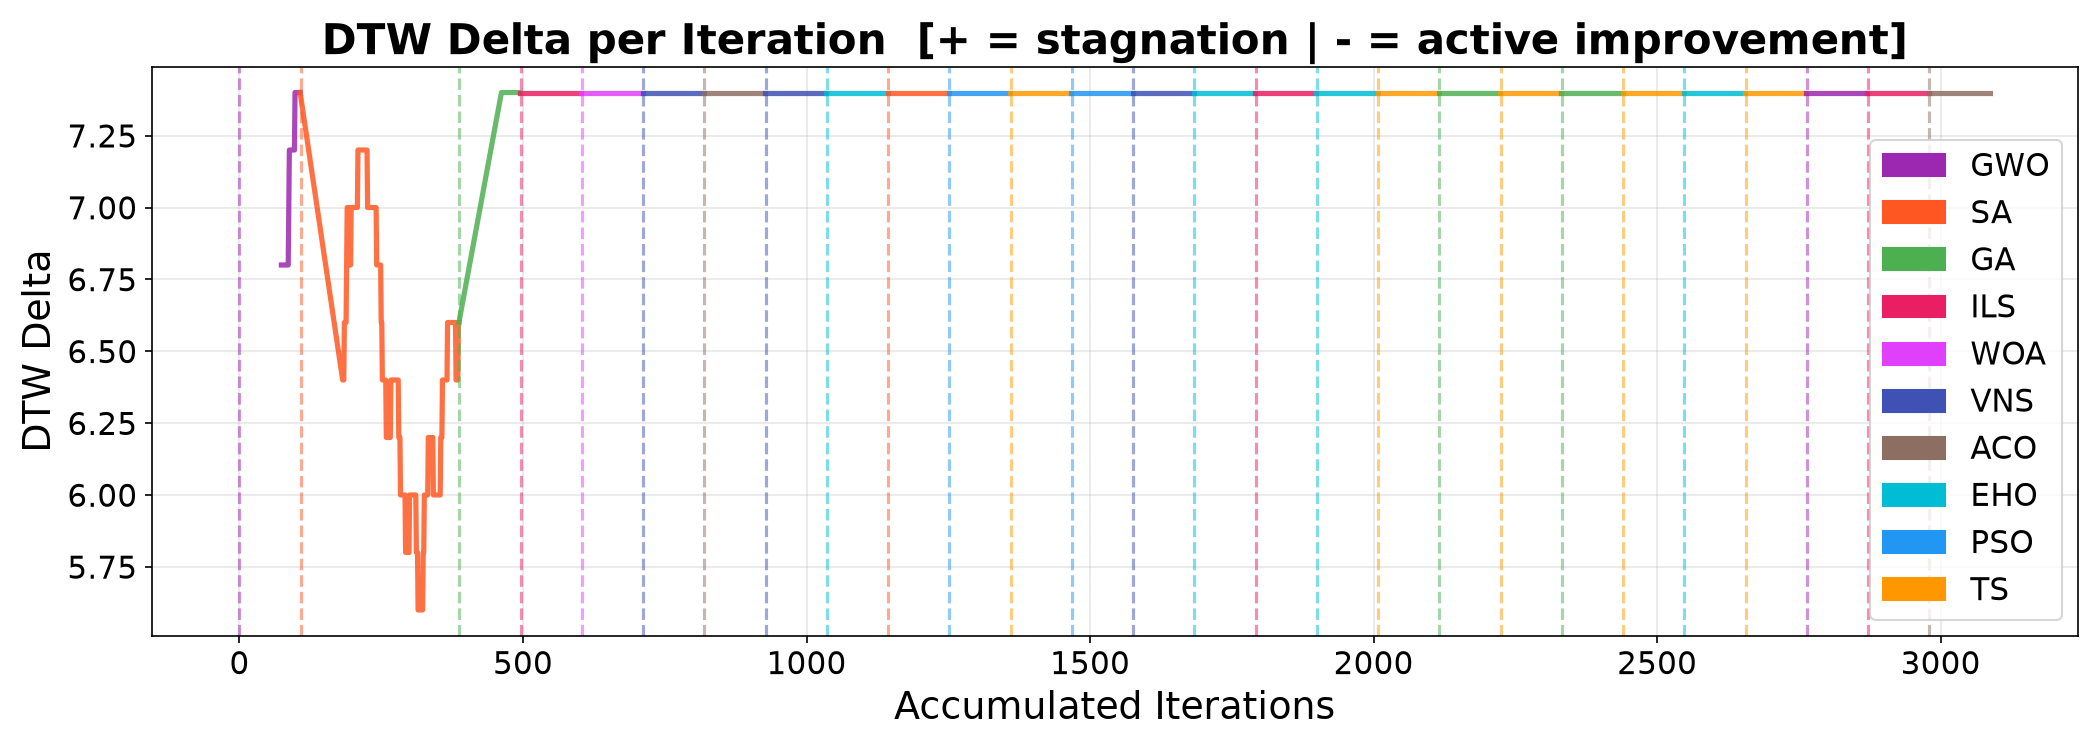
\includegraphics[width=0.32\textwidth]{imagenes_paper/mkp_ddtw_3k_mknapcb2_delta.png}}
\caption{Diagnostic suite for instance \textbf{mknapcb2} ($n=250$, $m=5$) under the DDTW framework with $T_{\max}=3{,}000$: (a)~final-fitness distribution over $N=31$ runs; (b)~convergence trajectory of the best run; (c)~elastic warping profile $\Delta$.}
\label{fig:mkp-best-cb2}
\end{figure}

% --- mknapcb3: DTW, 3,000 iterations ---
\begin{figure}[htbp]
\centering
\subfloat[Metaheuristic comparison.]{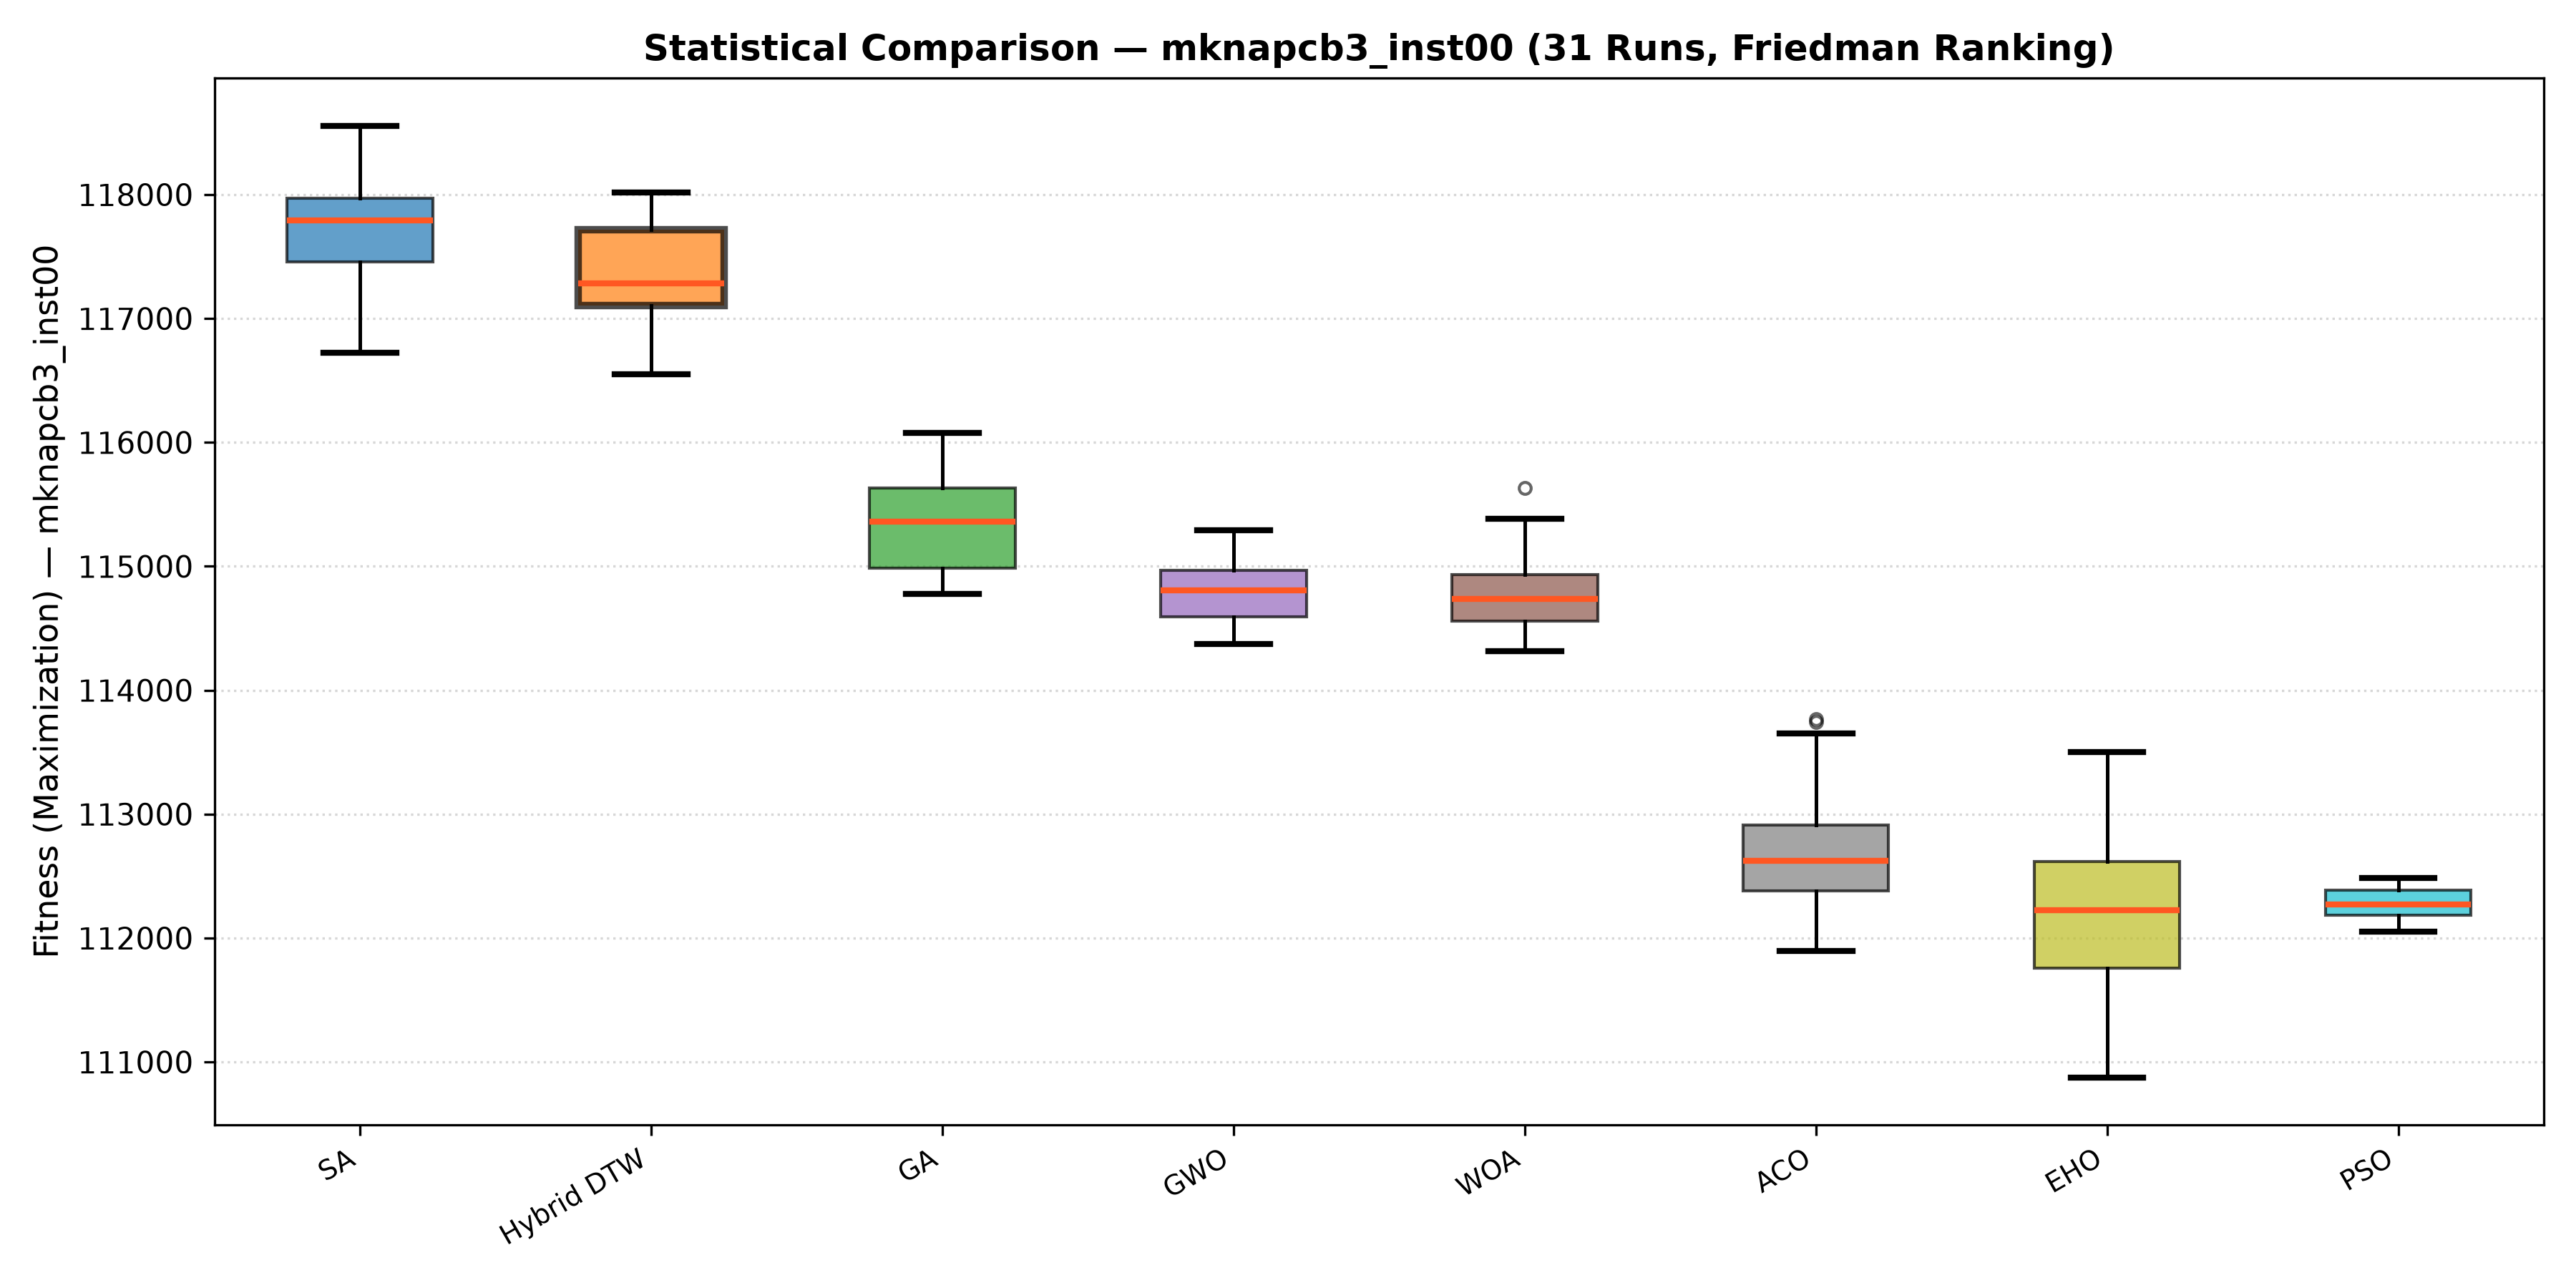
\includegraphics[width=0.32\textwidth]{imagenes_paper/mkp_dtw_3k_mknapcb3_comparativo_mh.png}}\hfill
\subfloat[Best-run convergence.]{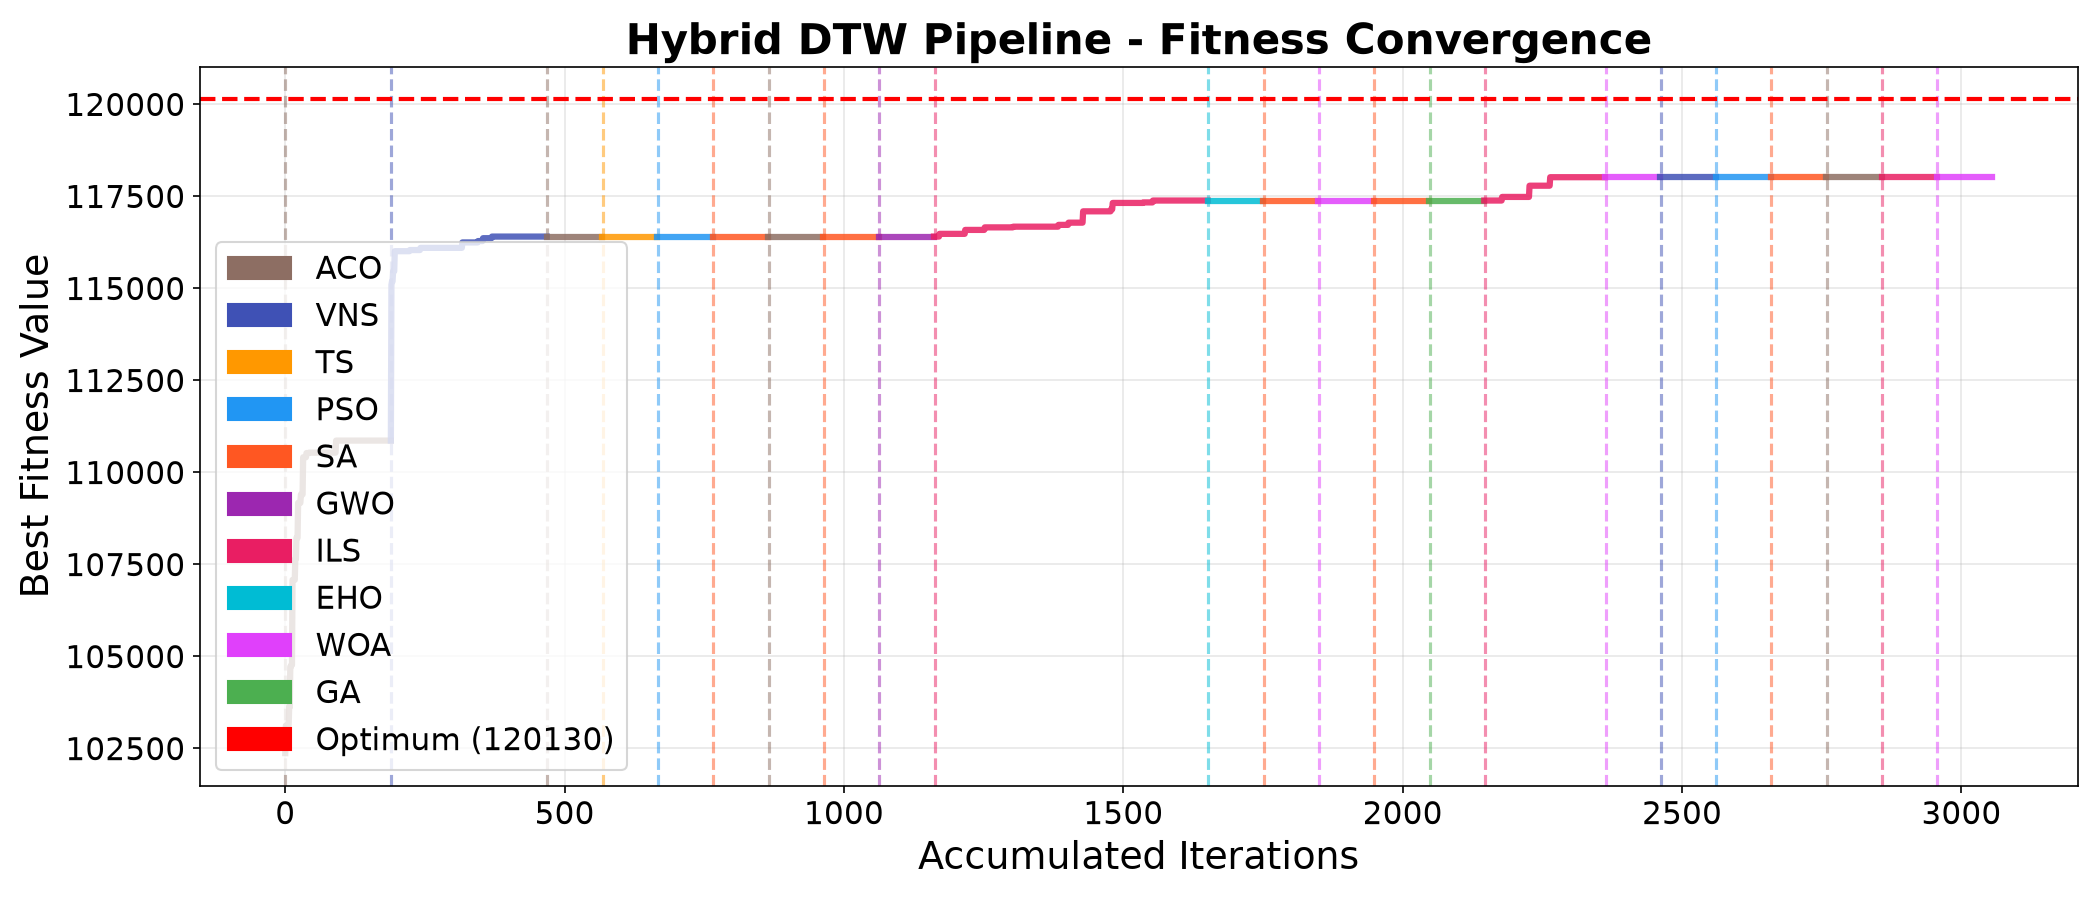
\includegraphics[width=0.32\textwidth]{imagenes_paper/mkp_dtw_3k_mknapcb3_convergencia.png}}\hfill
\subfloat[Elastic metric $\Delta=D_1-D_2$.]{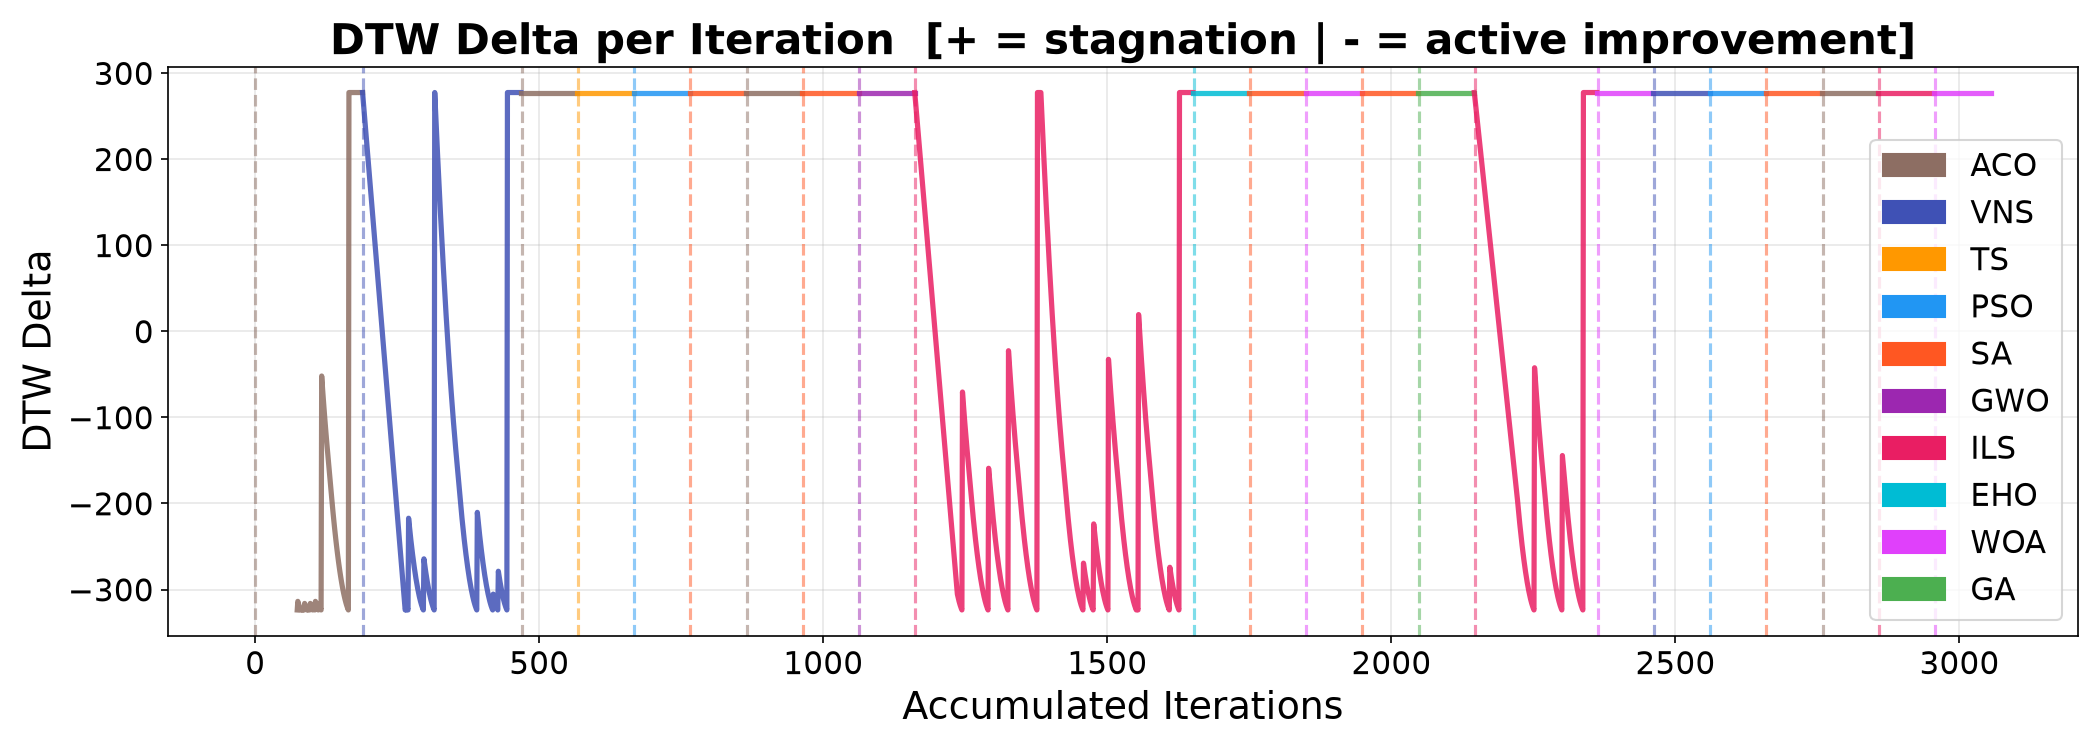
\includegraphics[width=0.32\textwidth]{imagenes_paper/mkp_dtw_3k_mknapcb3_delta.png}}
\caption{Diagnostic suite for instance \textbf{mknapcb3} ($n=500$, $m=5$) under the DTW framework with $T_{\max}=3{,}000$: (a)~final-fitness distribution over $N=31$ runs; (b)~convergence trajectory of the best run; (c)~elastic warping profile $\Delta$.}
\label{fig:mkp-best-cb3}
\end{figure}

% --- mknapcb4: DTW, 3,000 iterations ---
\begin{figure}[htbp]
\centering
\subfloat[Metaheuristic comparison.]{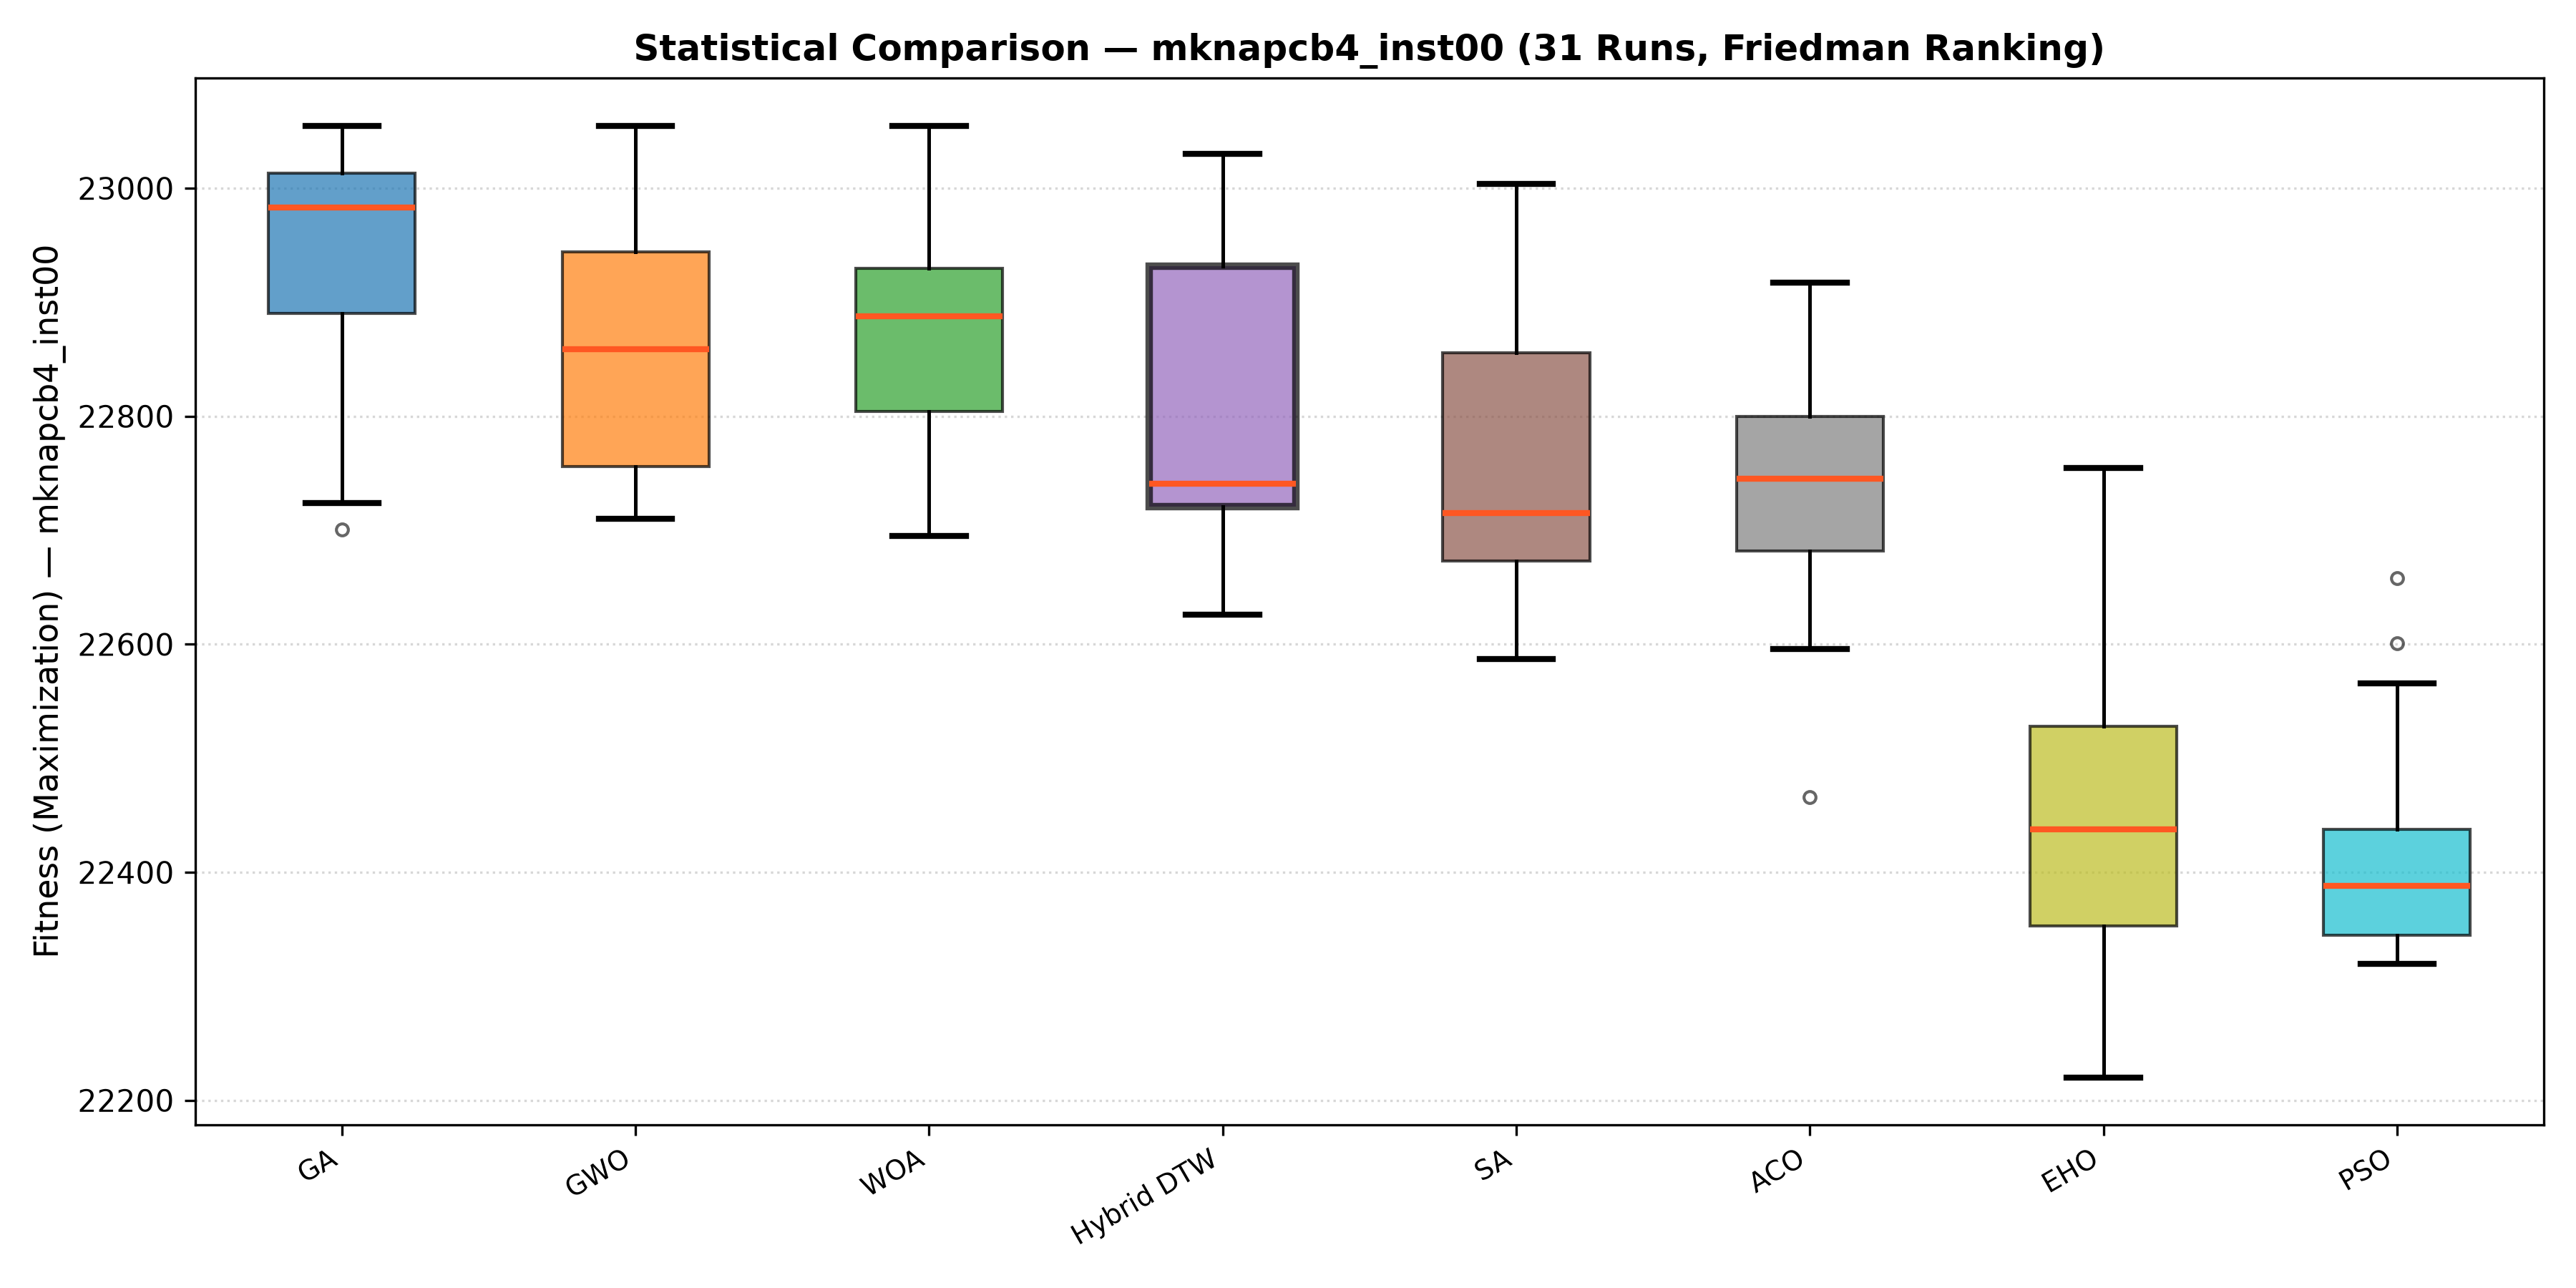
\includegraphics[width=0.32\textwidth]{imagenes_paper/mkp_dtw_3k_mknapcb4_comparativo_mh.png}}\hfill
\subfloat[Best-run convergence.]{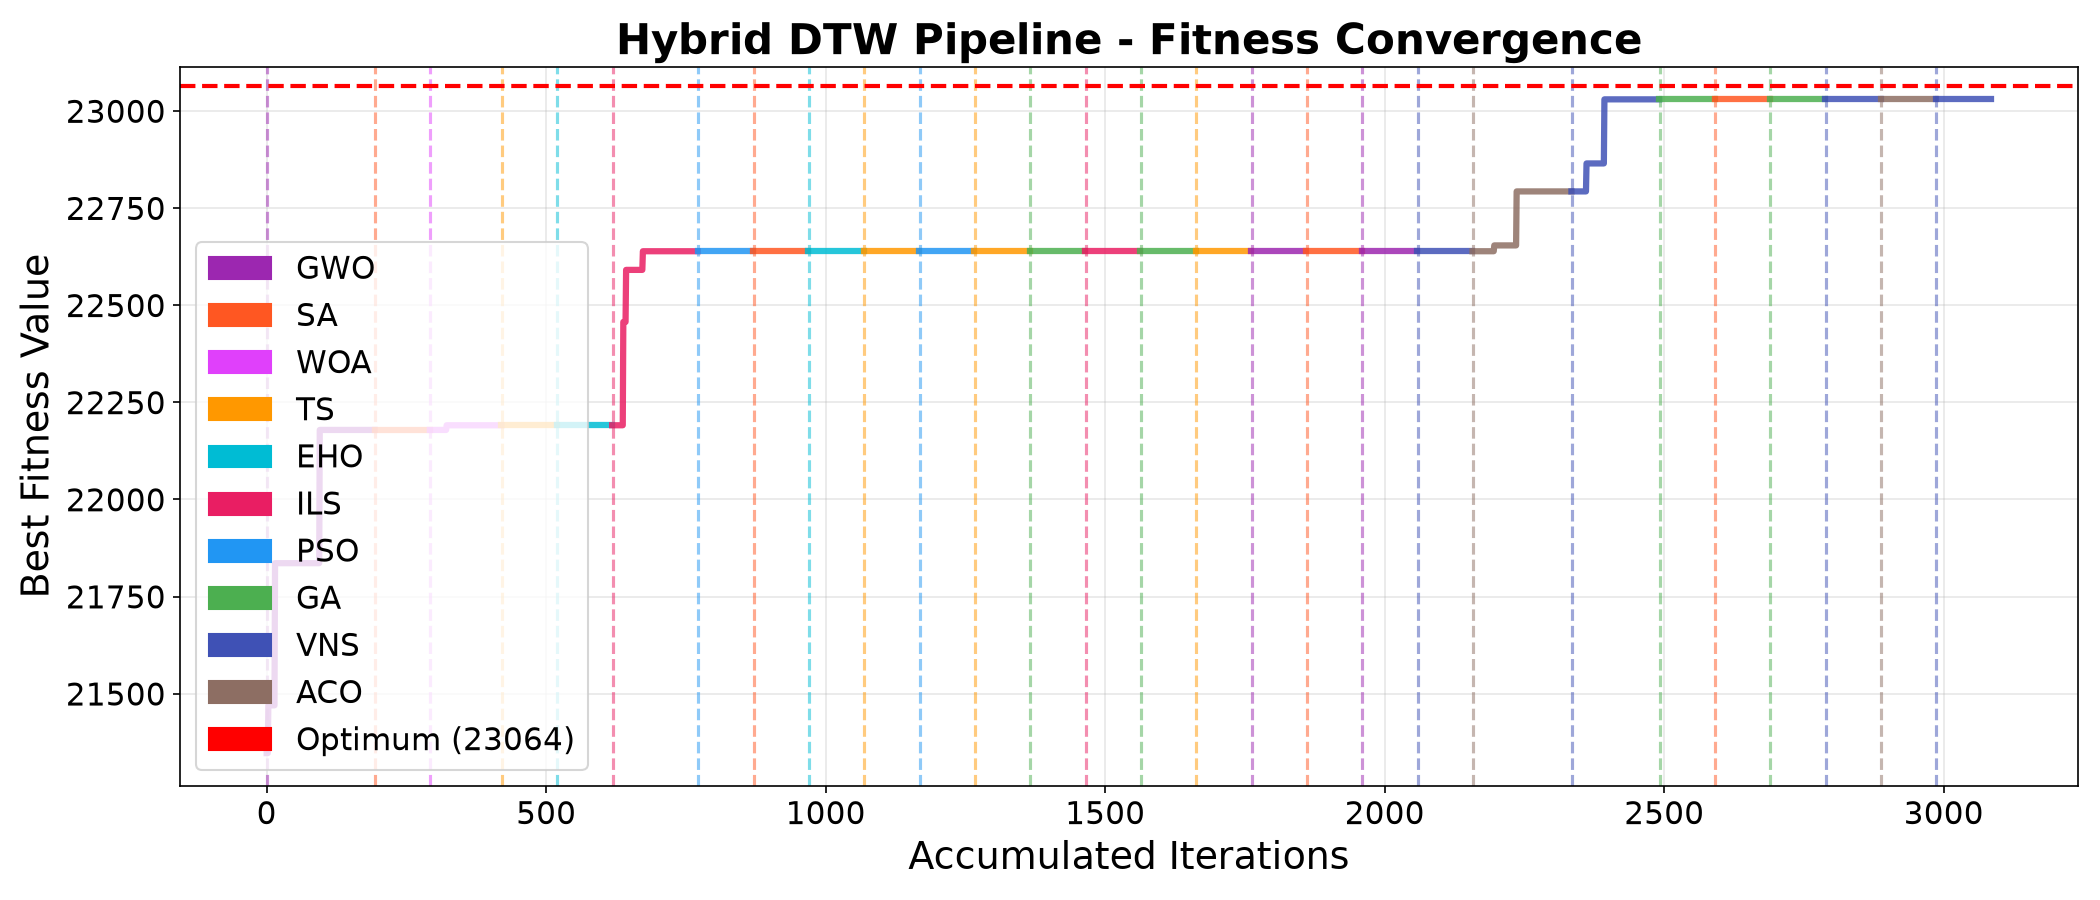
\includegraphics[width=0.32\textwidth]{imagenes_paper/mkp_dtw_3k_mknapcb4_convergencia.png}}\hfill
\subfloat[Elastic metric $\Delta=D_1-D_2$.]{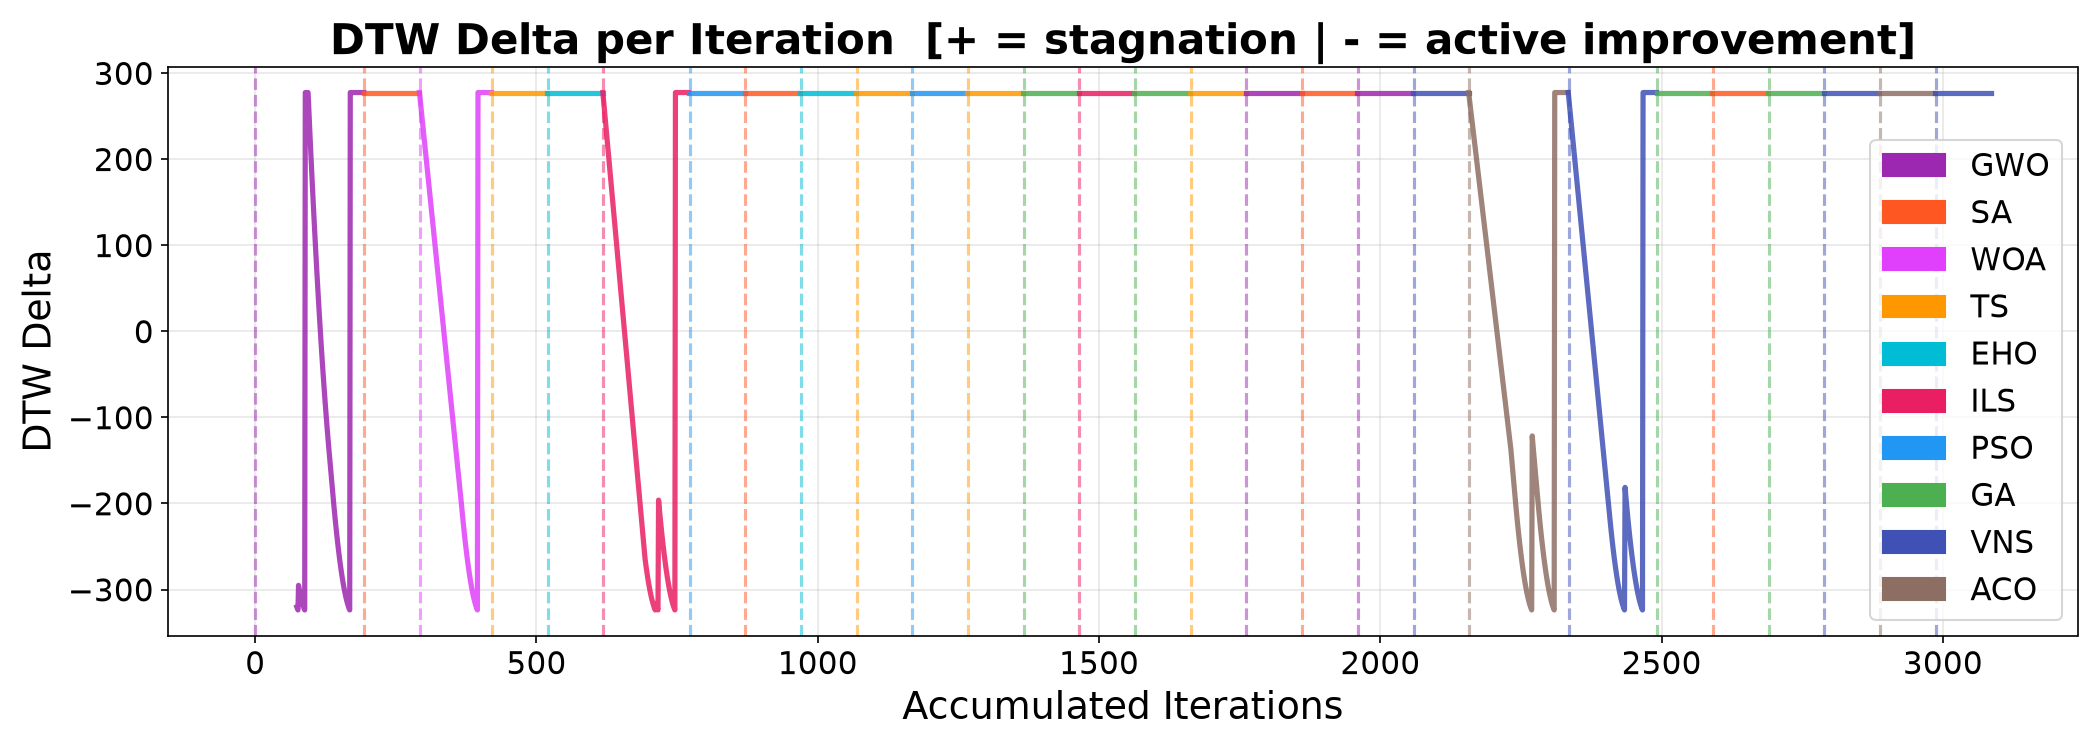
\includegraphics[width=0.32\textwidth]{imagenes_paper/mkp_dtw_3k_mknapcb4_delta.png}}
\caption{Diagnostic suite for instance \textbf{mknapcb4} ($n=100$, $m=10$) under the DTW framework with $T_{\max}=3{,}000$: (a)~final-fitness distribution over $N=31$ runs; (b)~convergence trajectory of the best run; (c)~elastic warping profile $\Delta$.}
\label{fig:mkp-best-cb4}
\end{figure}

% --- mknapcb5: DTW, 3,000 iterations ---
\begin{figure}[htbp]
\centering
\subfloat[Metaheuristic comparison.]{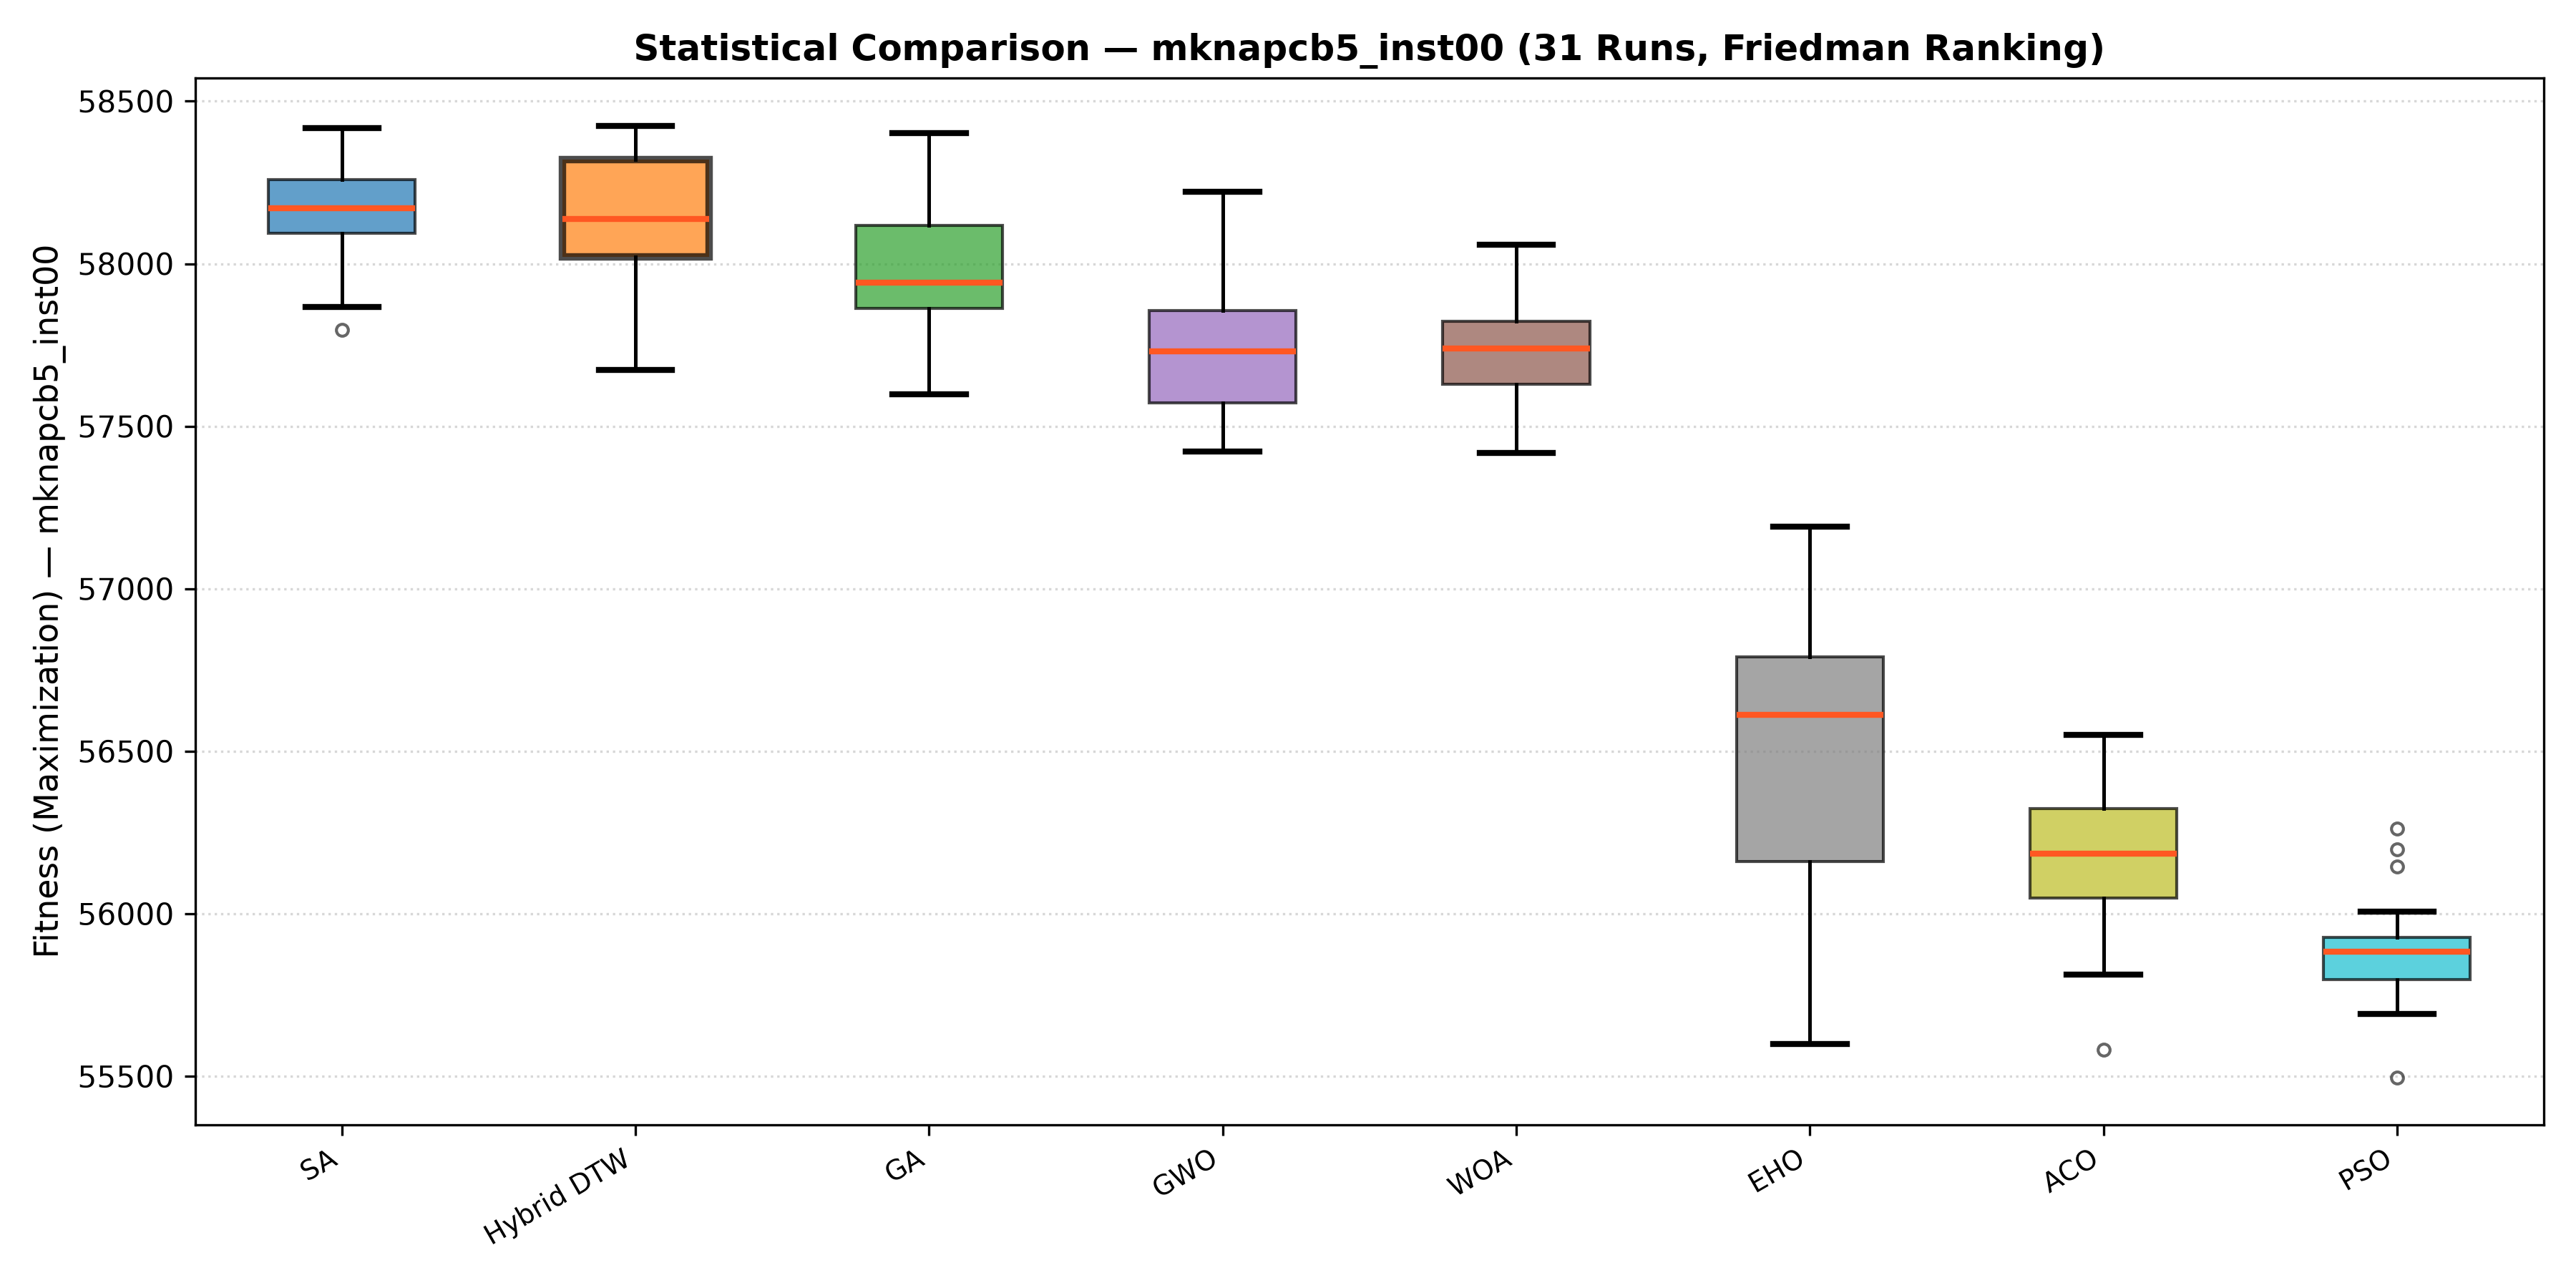
\includegraphics[width=0.32\textwidth]{imagenes_paper/mkp_dtw_3k_mknapcb5_comparativo_mh.png}}\hfill
\subfloat[Best-run convergence.]{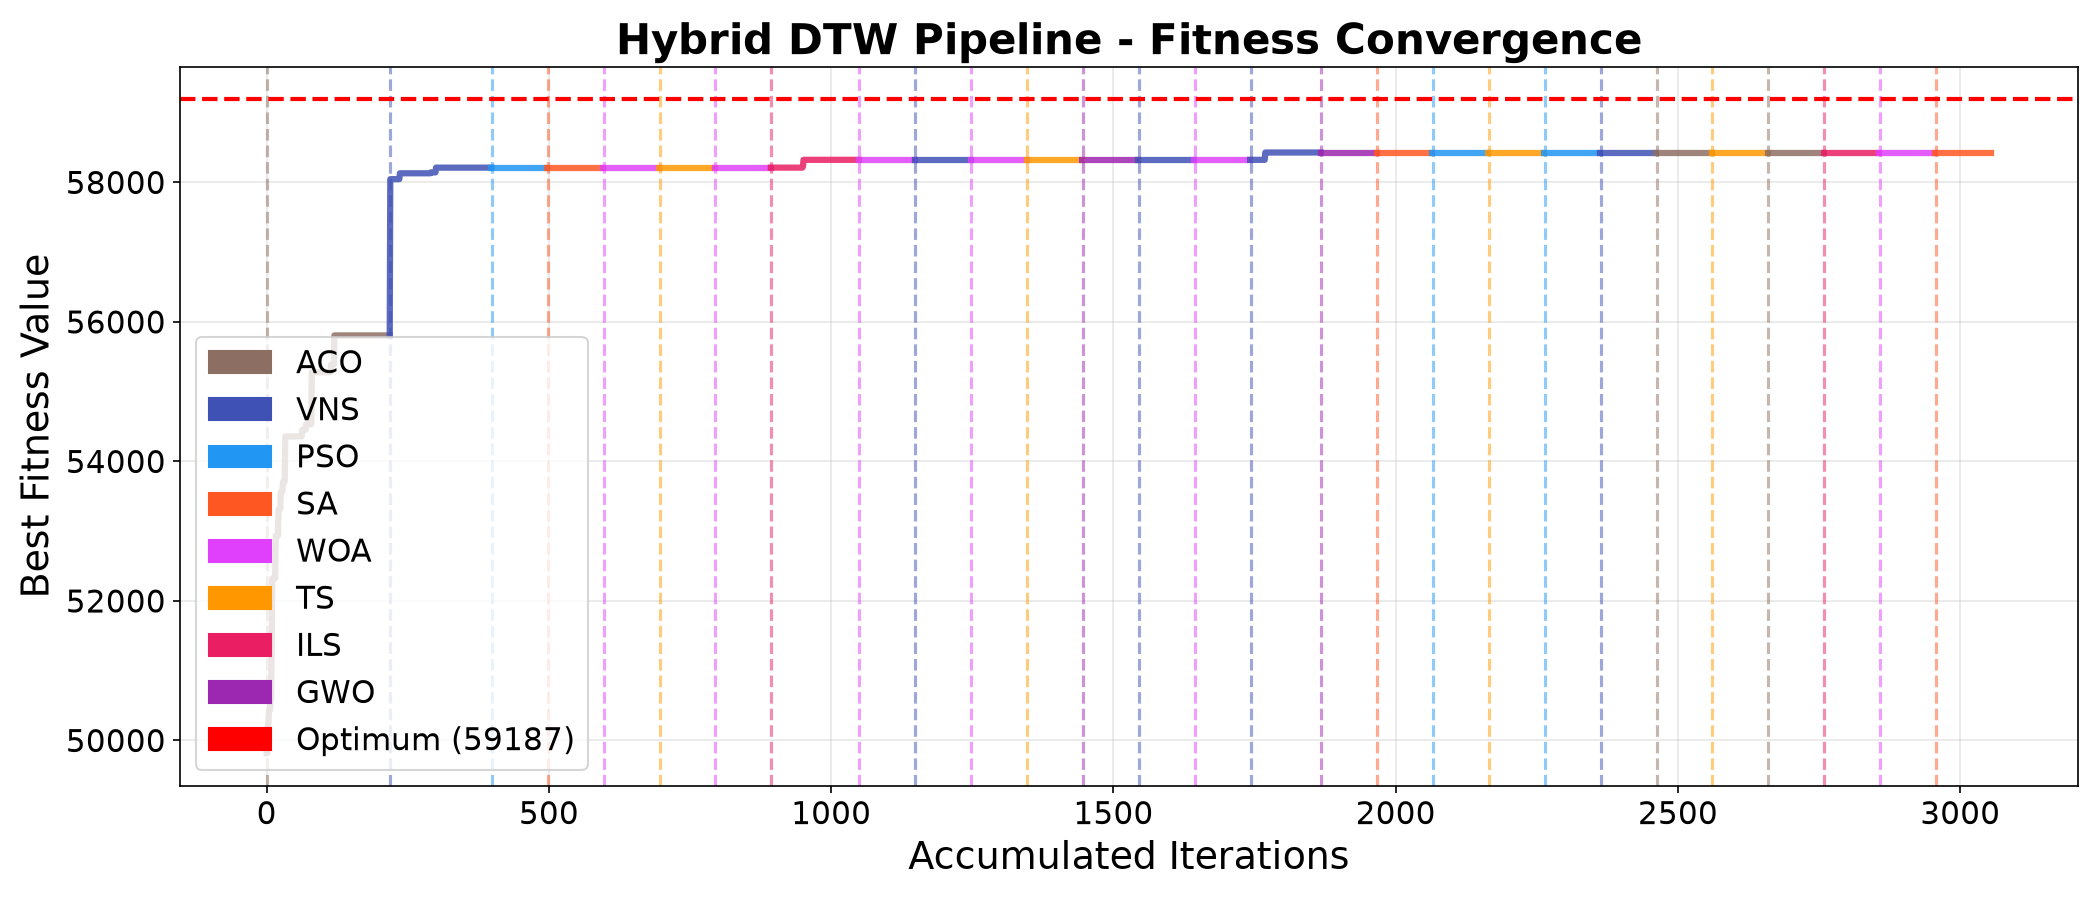
\includegraphics[width=0.32\textwidth]{imagenes_paper/mkp_dtw_3k_mknapcb5_convergencia.png}}\hfill
\subfloat[Elastic metric $\Delta=D_1-D_2$.]{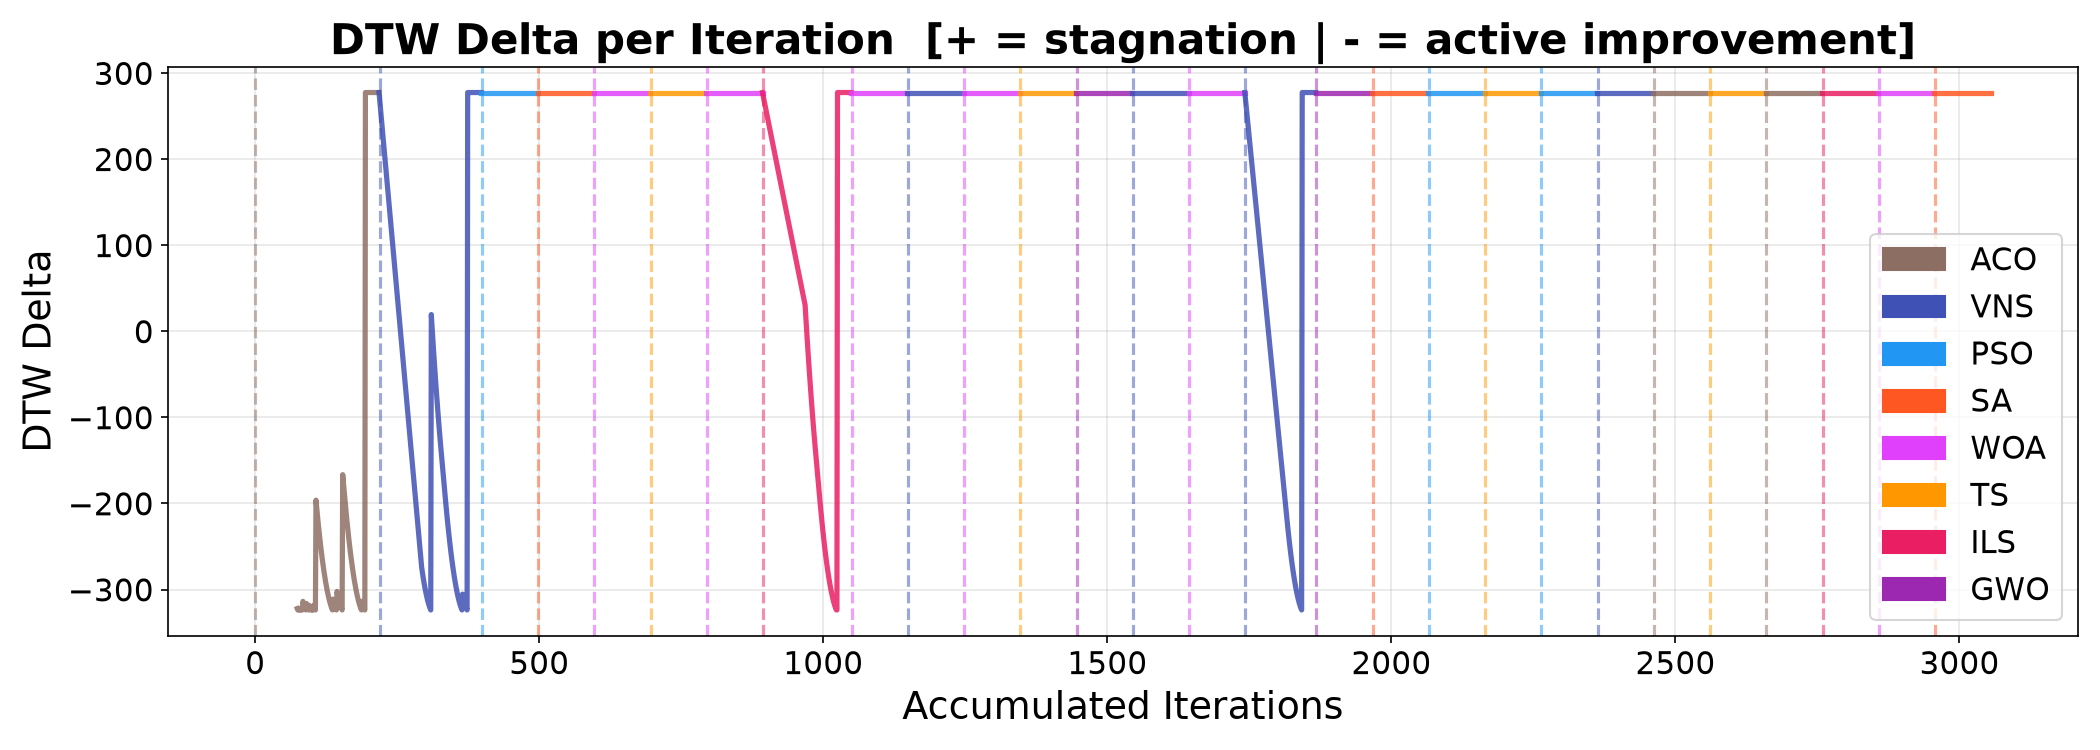
\includegraphics[width=0.32\textwidth]{imagenes_paper/mkp_dtw_3k_mknapcb5_delta.png}}
\caption{Diagnostic suite for instance \textbf{mknapcb5} ($n=250$, $m=10$) under the DTW framework with $T_{\max}=3{,}000$: (a)~final-fitness distribution over $N=31$ runs; (b)~convergence trajectory of the best run; (c)~elastic warping profile $\Delta$.}
\label{fig:mkp-best-cb5}
\end{figure}

% --- mknapcb6: DTW, 3,000 iterations ---
\begin{figure}[htbp]
\centering
\subfloat[Metaheuristic comparison.]{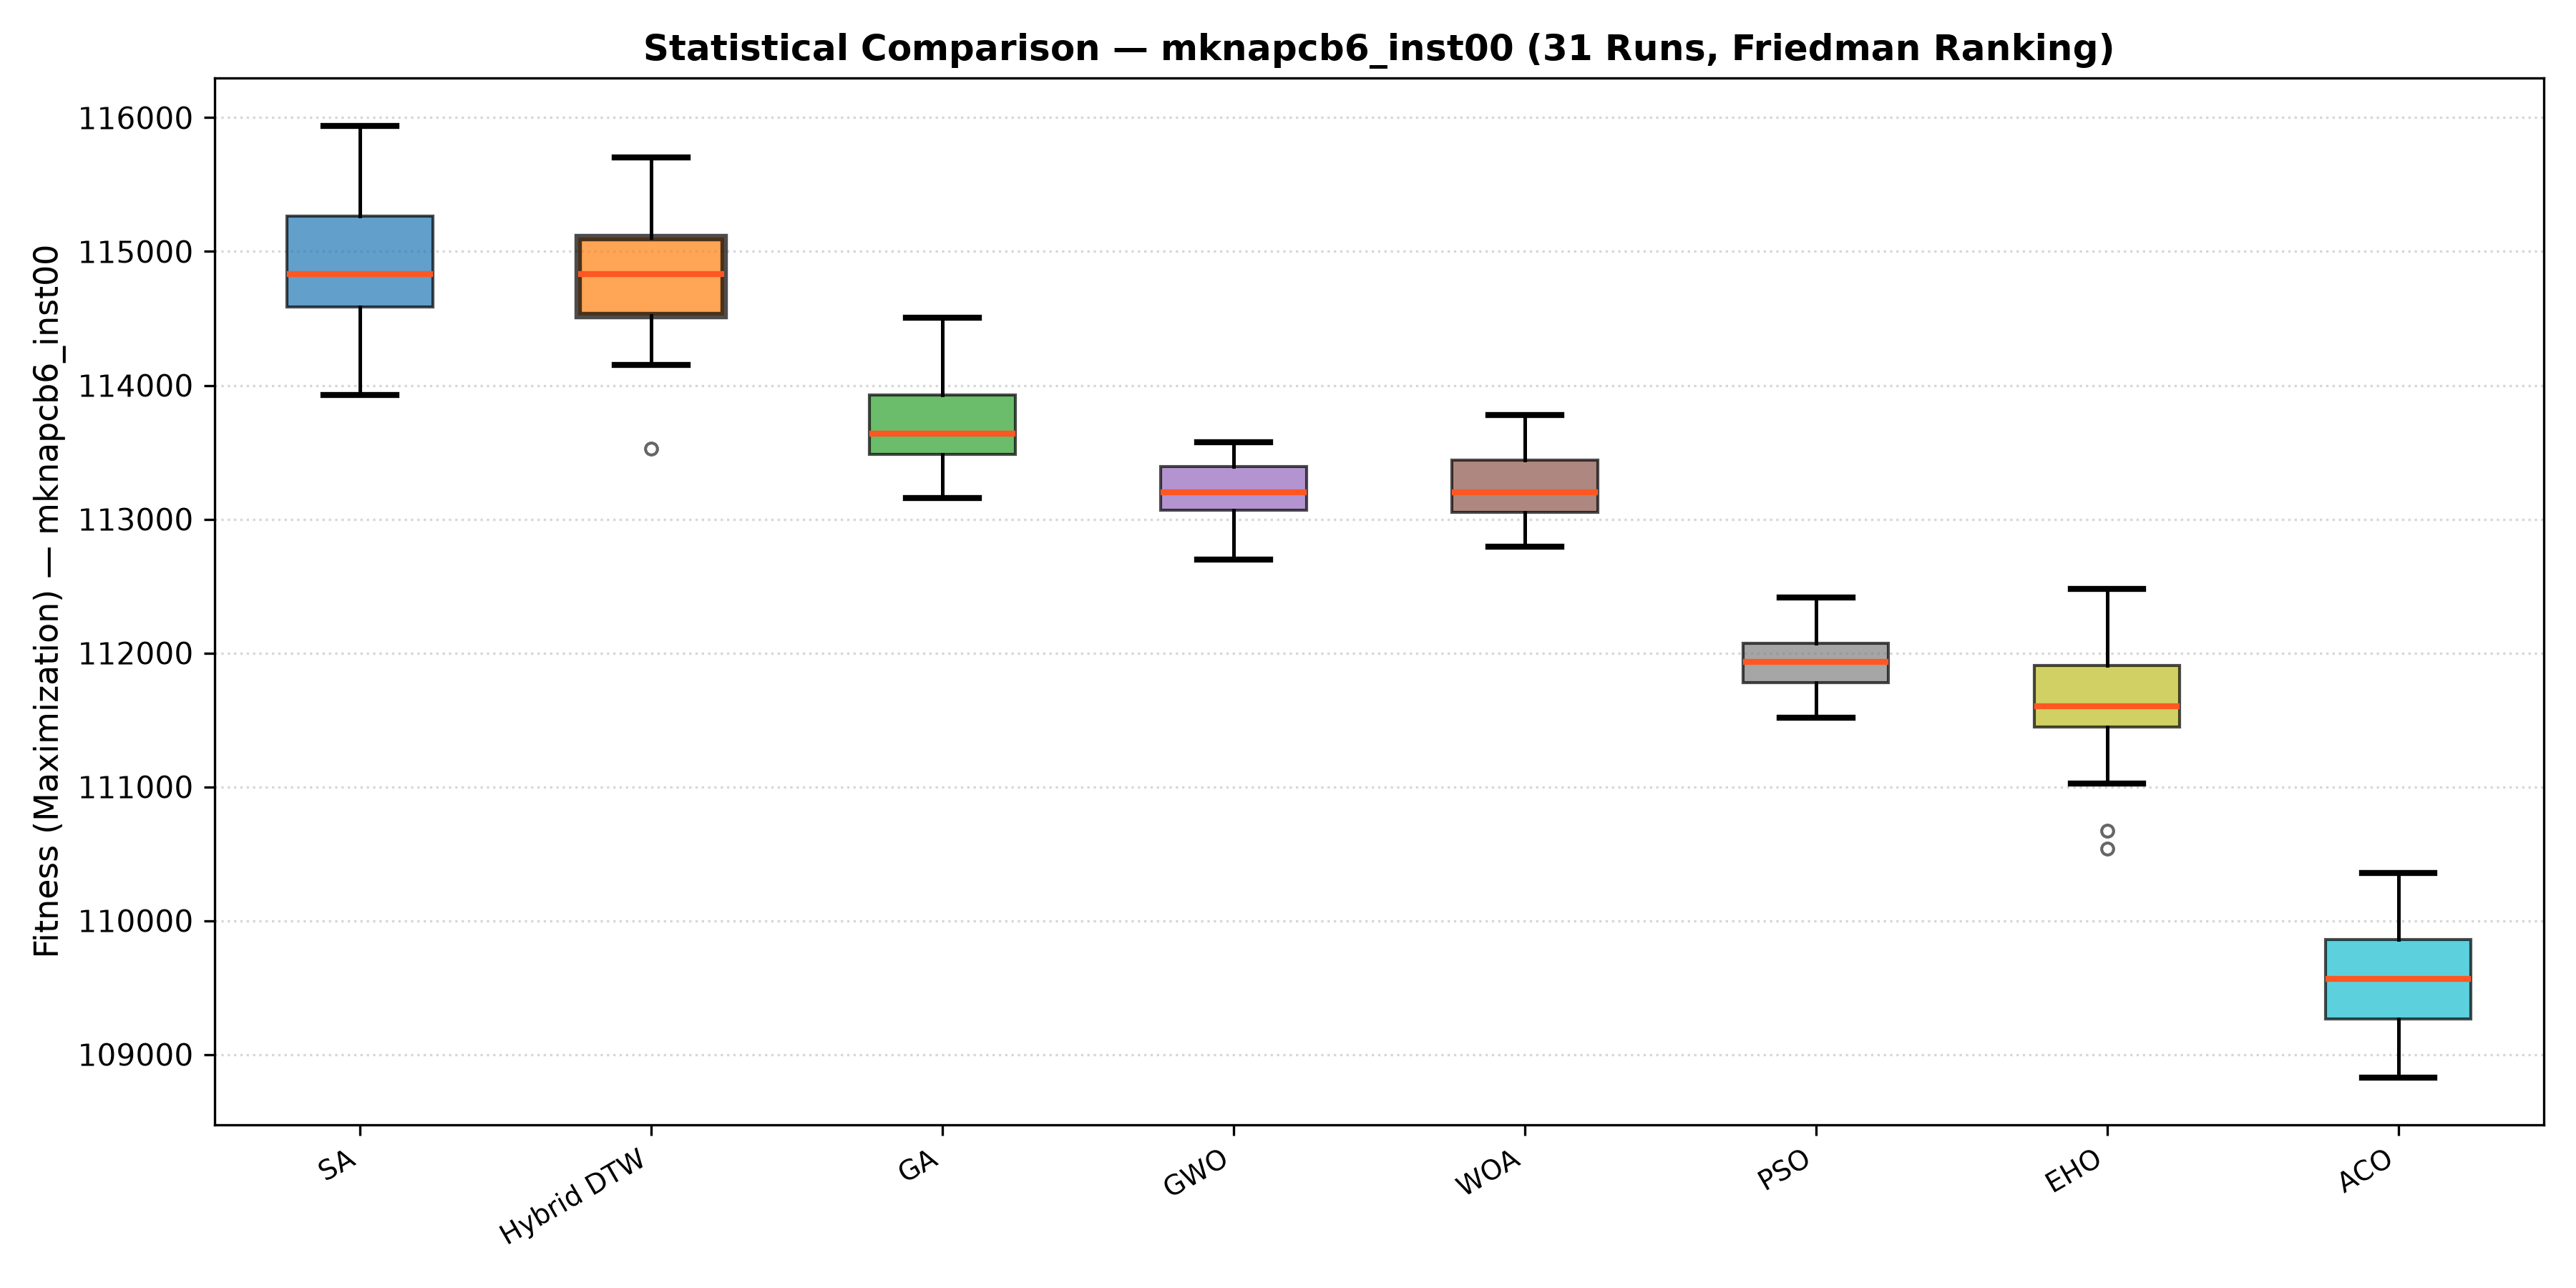
\includegraphics[width=0.32\textwidth]{imagenes_paper/mkp_dtw_3k_mknapcb6_comparativo_mh.png}}\hfill
\subfloat[Best-run convergence.]{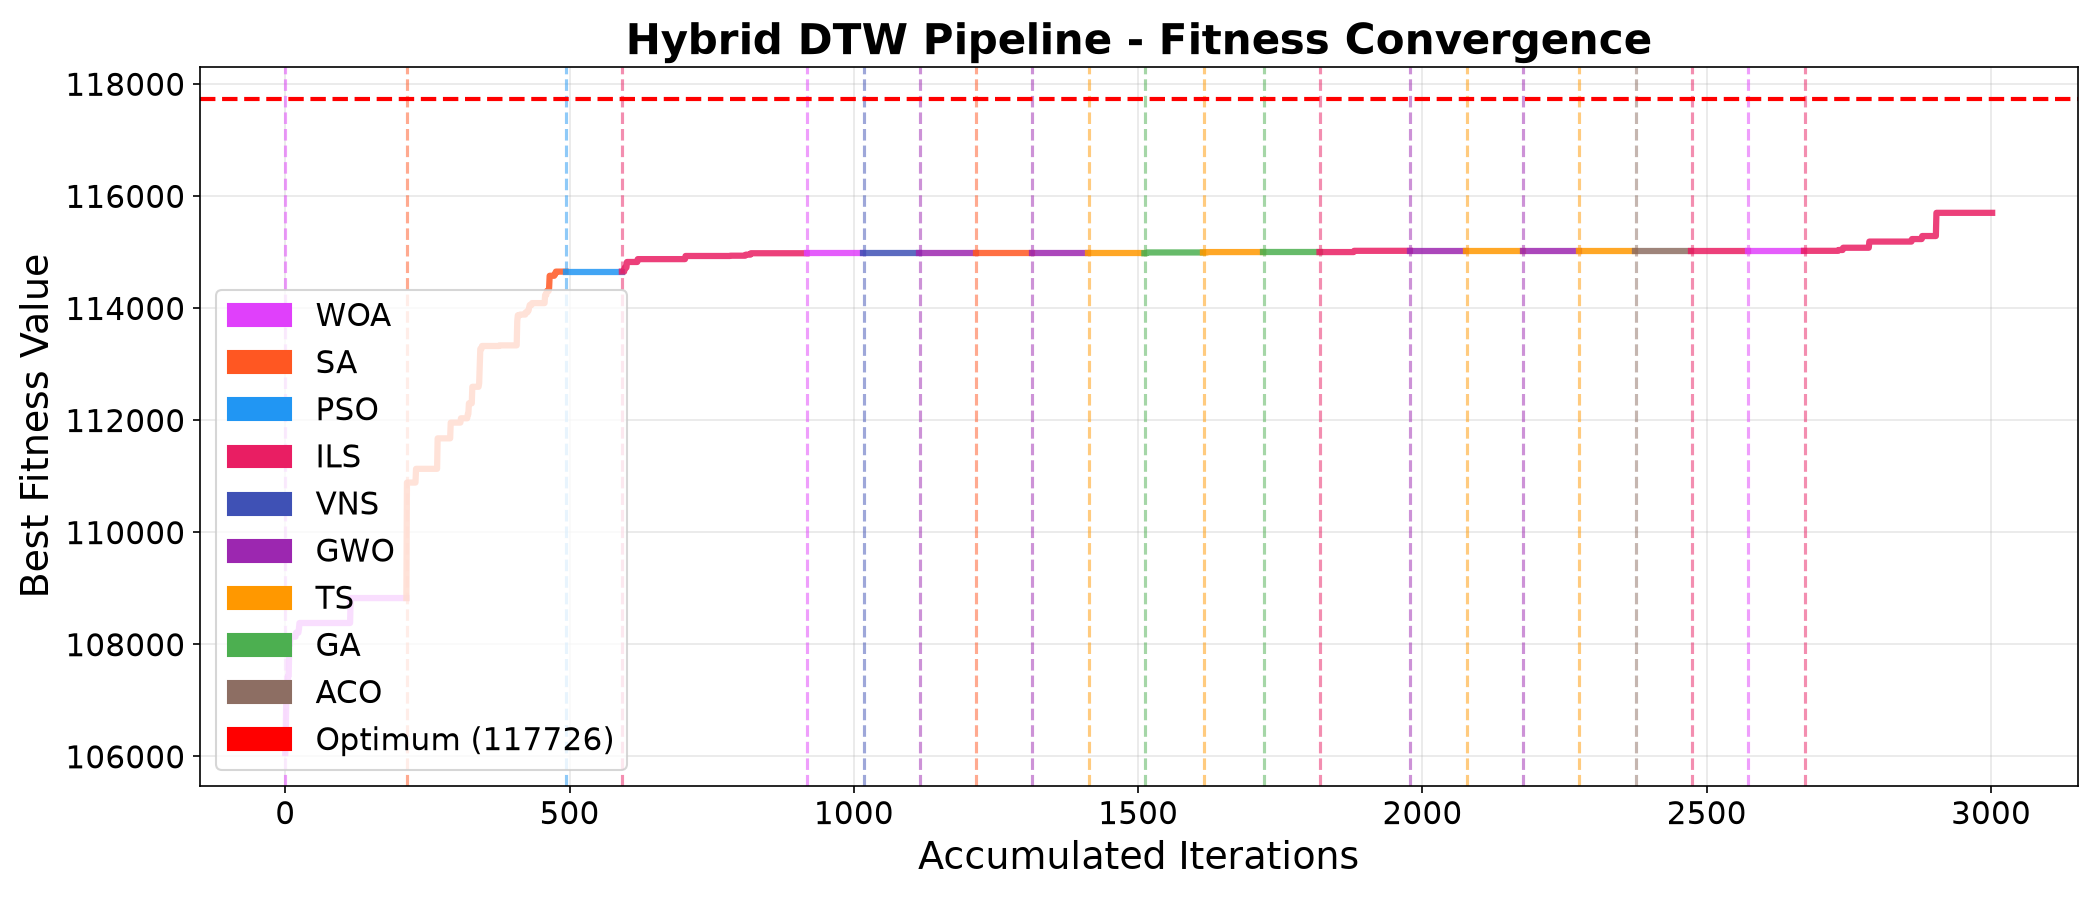
\includegraphics[width=0.32\textwidth]{imagenes_paper/mkp_dtw_3k_mknapcb6_convergencia.png}}\hfill
\subfloat[Elastic metric $\Delta=D_1-D_2$.]{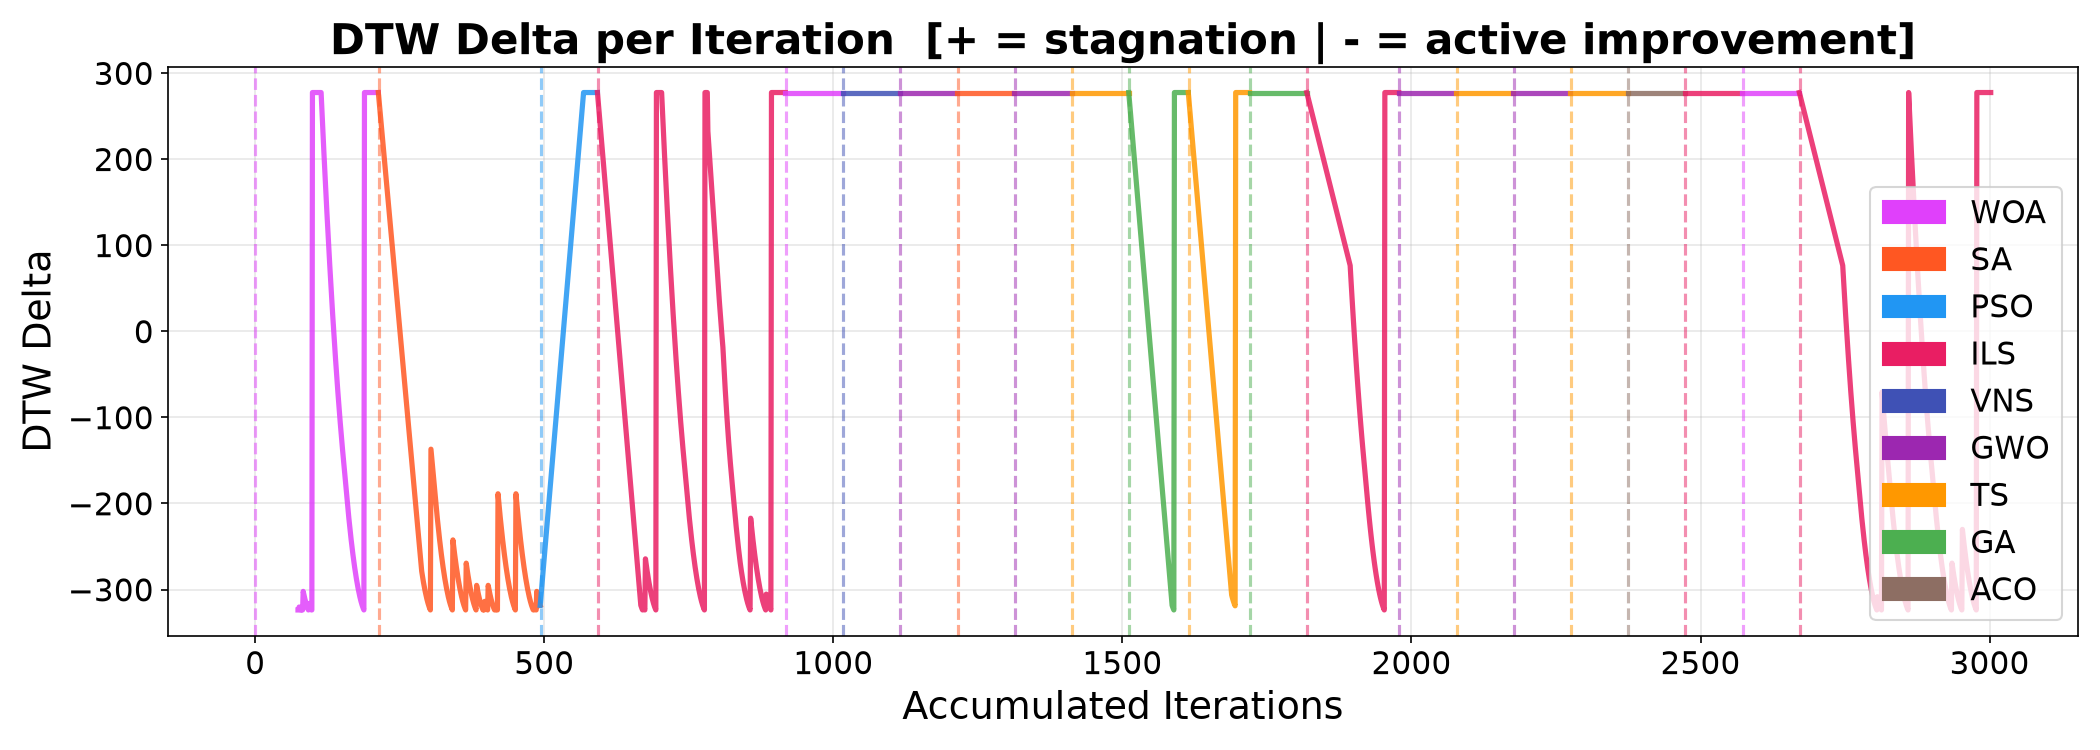
\includegraphics[width=0.32\textwidth]{imagenes_paper/mkp_dtw_3k_mknapcb6_delta.png}}
\caption{Diagnostic suite for instance \textbf{mknapcb6} ($n=500$, $m=10$) under the DTW framework with $T_{\max}=3{,}000$: (a)~final-fitness distribution over $N=31$ runs; (b)~convergence trajectory of the best run; (c)~elastic warping profile $\Delta$.}
\label{fig:mkp-best-cb6}
\end{figure}

% --- mknapcb7: DTW, 3,000 iterations ---
\begin{figure}[htbp]
\centering
\subfloat[Metaheuristic comparison.]{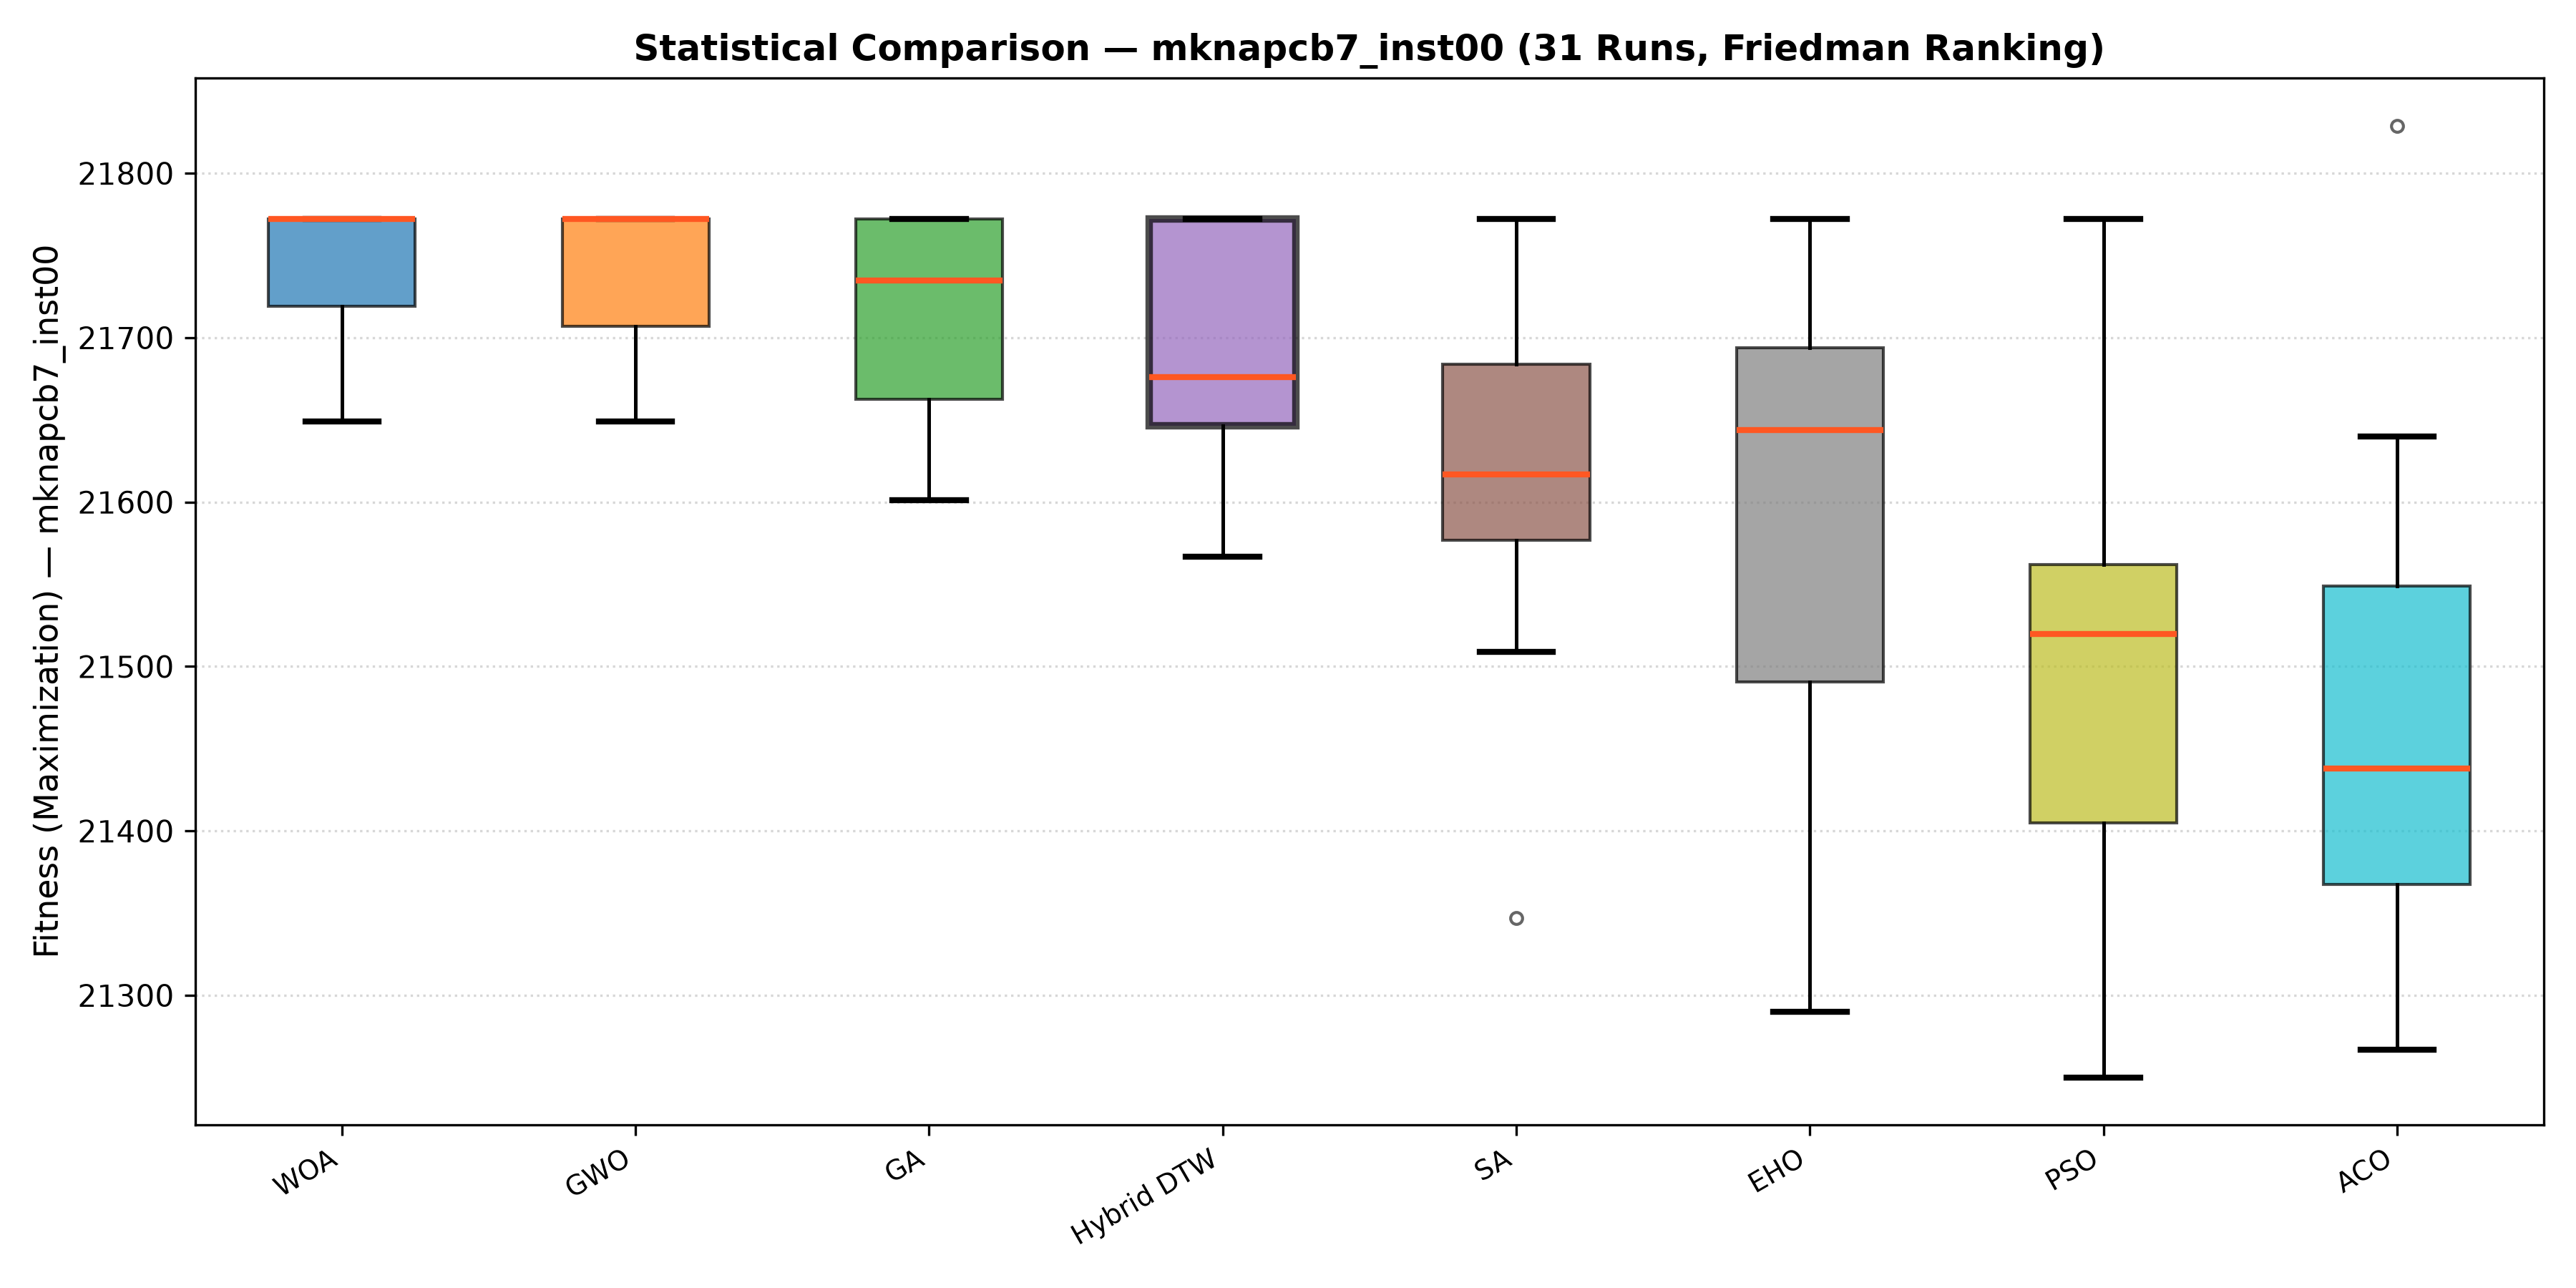
\includegraphics[width=0.32\textwidth]{imagenes_paper/mkp_dtw_3k_mknapcb7_comparativo_mh.png}}\hfill
\subfloat[Best-run convergence.]{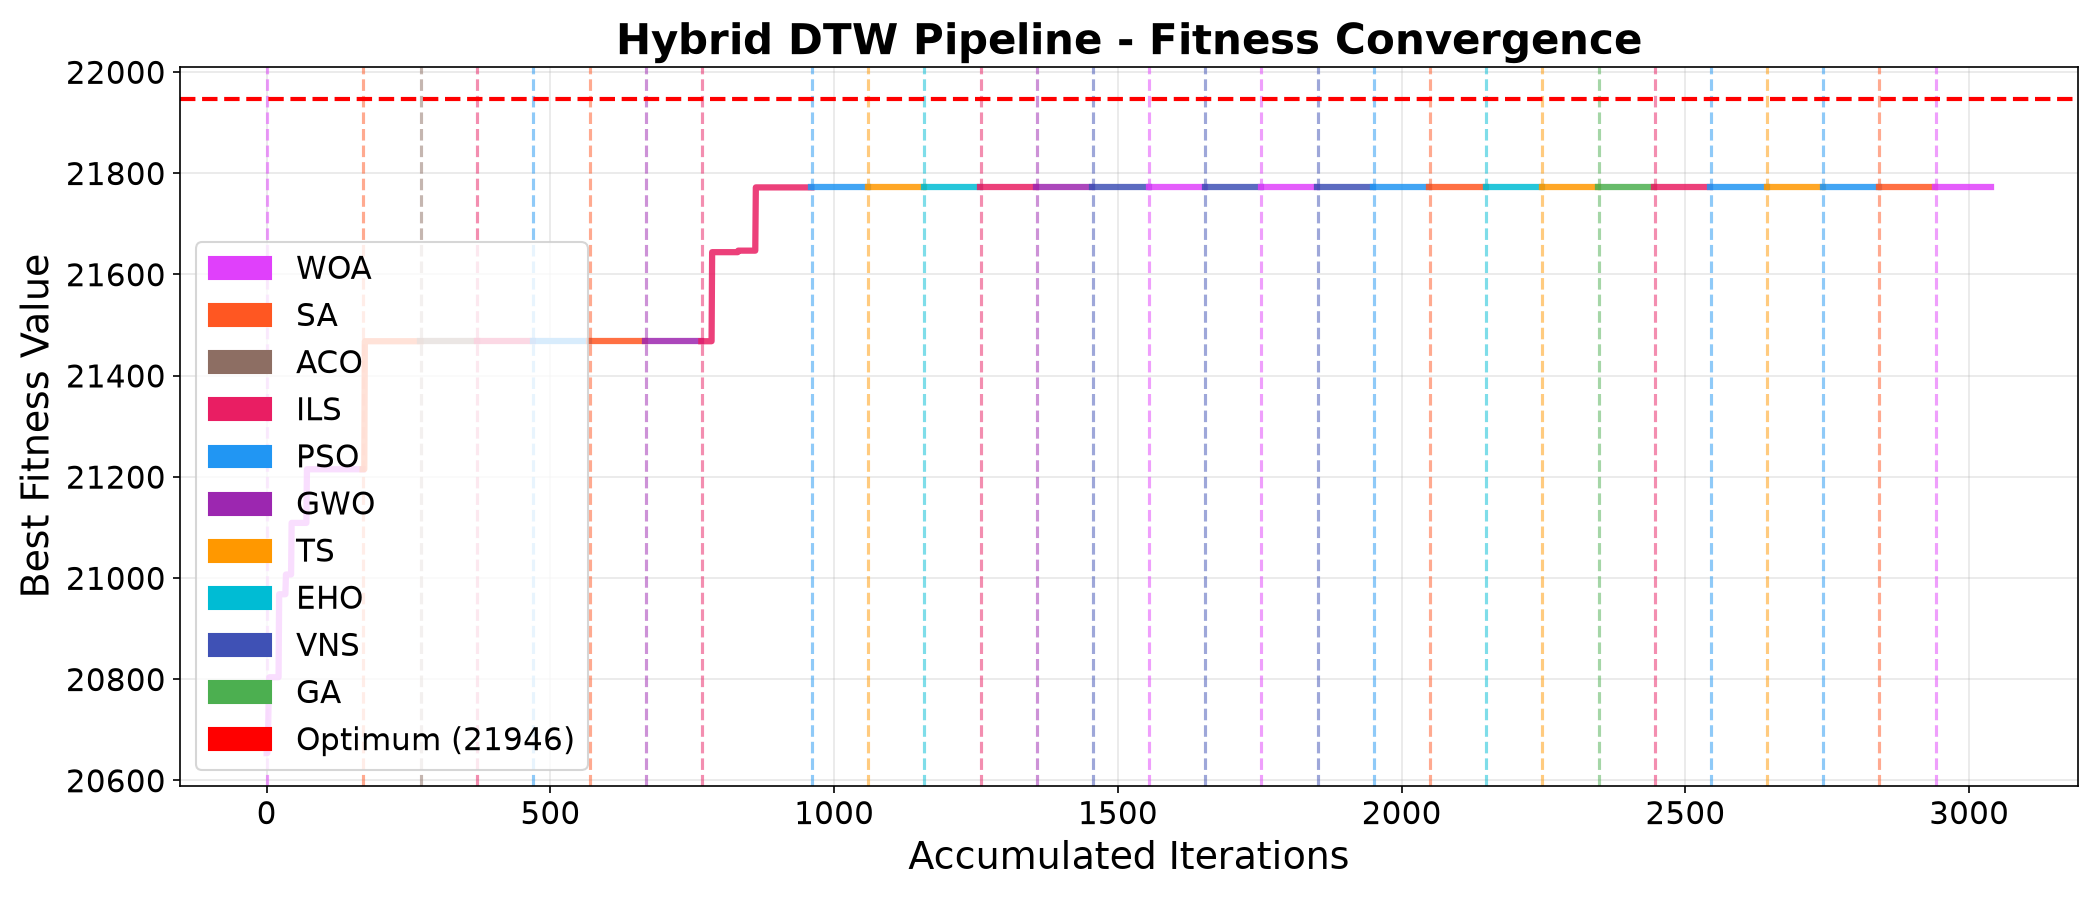
\includegraphics[width=0.32\textwidth]{imagenes_paper/mkp_dtw_3k_mknapcb7_convergencia.png}}\hfill
\subfloat[Elastic metric $\Delta=D_1-D_2$.]{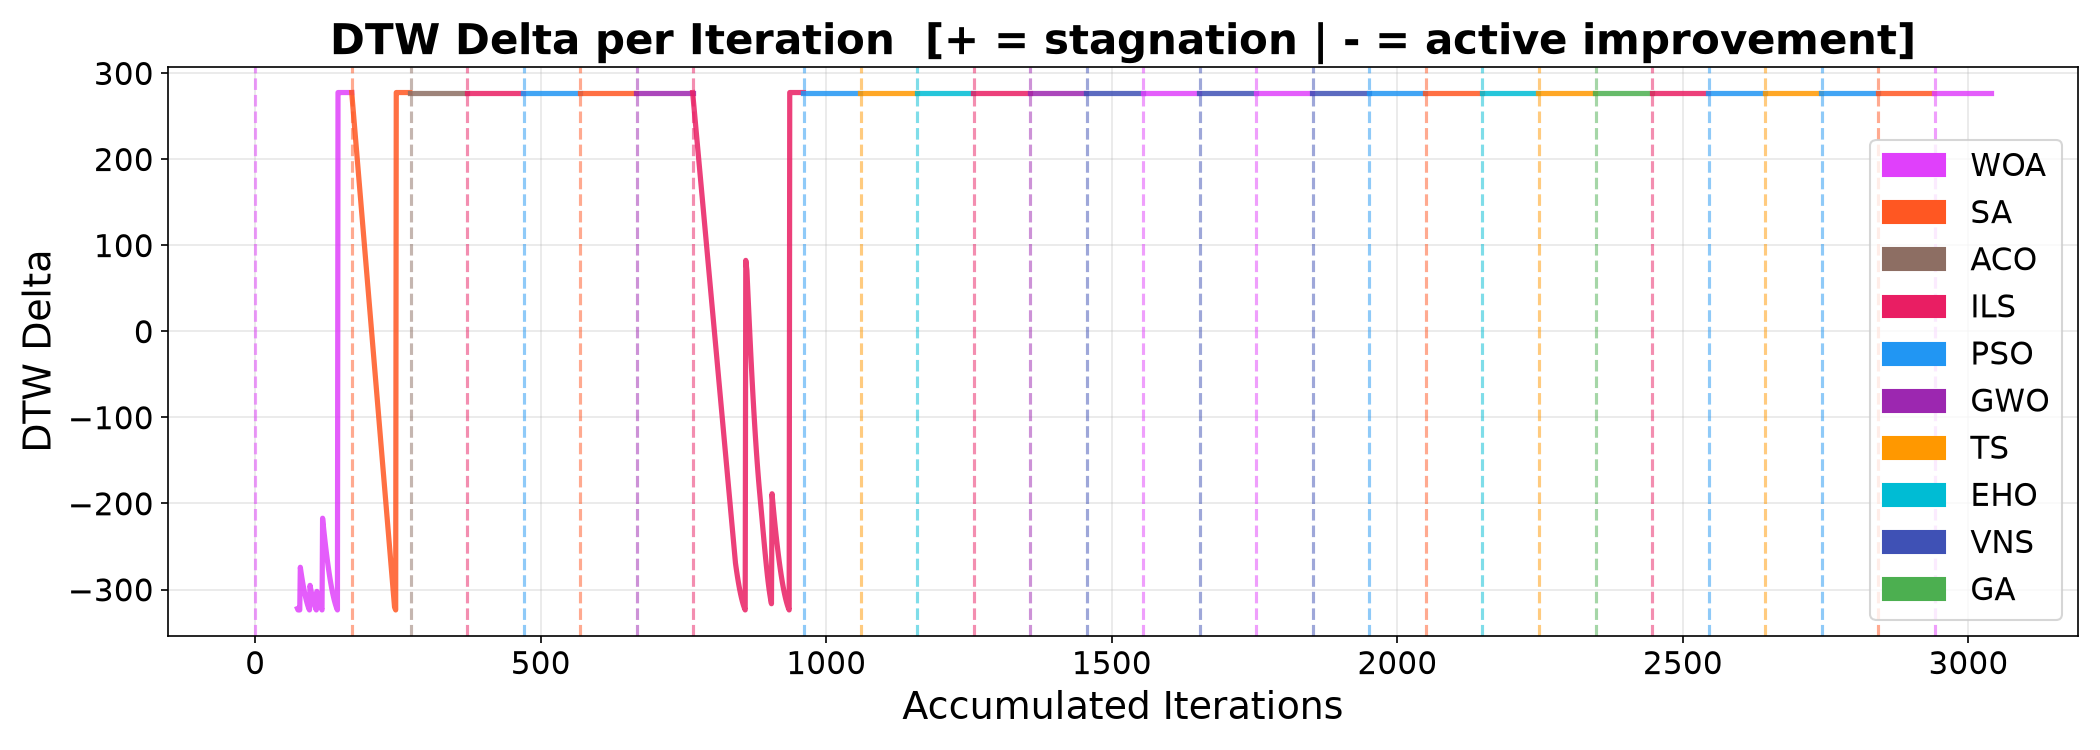
\includegraphics[width=0.32\textwidth]{imagenes_paper/mkp_dtw_3k_mknapcb7_delta.png}}
\caption{Diagnostic suite for instance \textbf{mknapcb7} ($n=100$, $m=30$) under the DTW framework with $T_{\max}=3{,}000$: (a)~final-fitness distribution over $N=31$ runs; (b)~convergence trajectory of the best run; (c)~elastic warping profile $\Delta$.}
\label{fig:mkp-best-cb7}
\end{figure}

% --- mknapcb8: DTW, 3,000 iterations ---
\begin{figure}[htbp]
\centering
\subfloat[Metaheuristic comparison.]{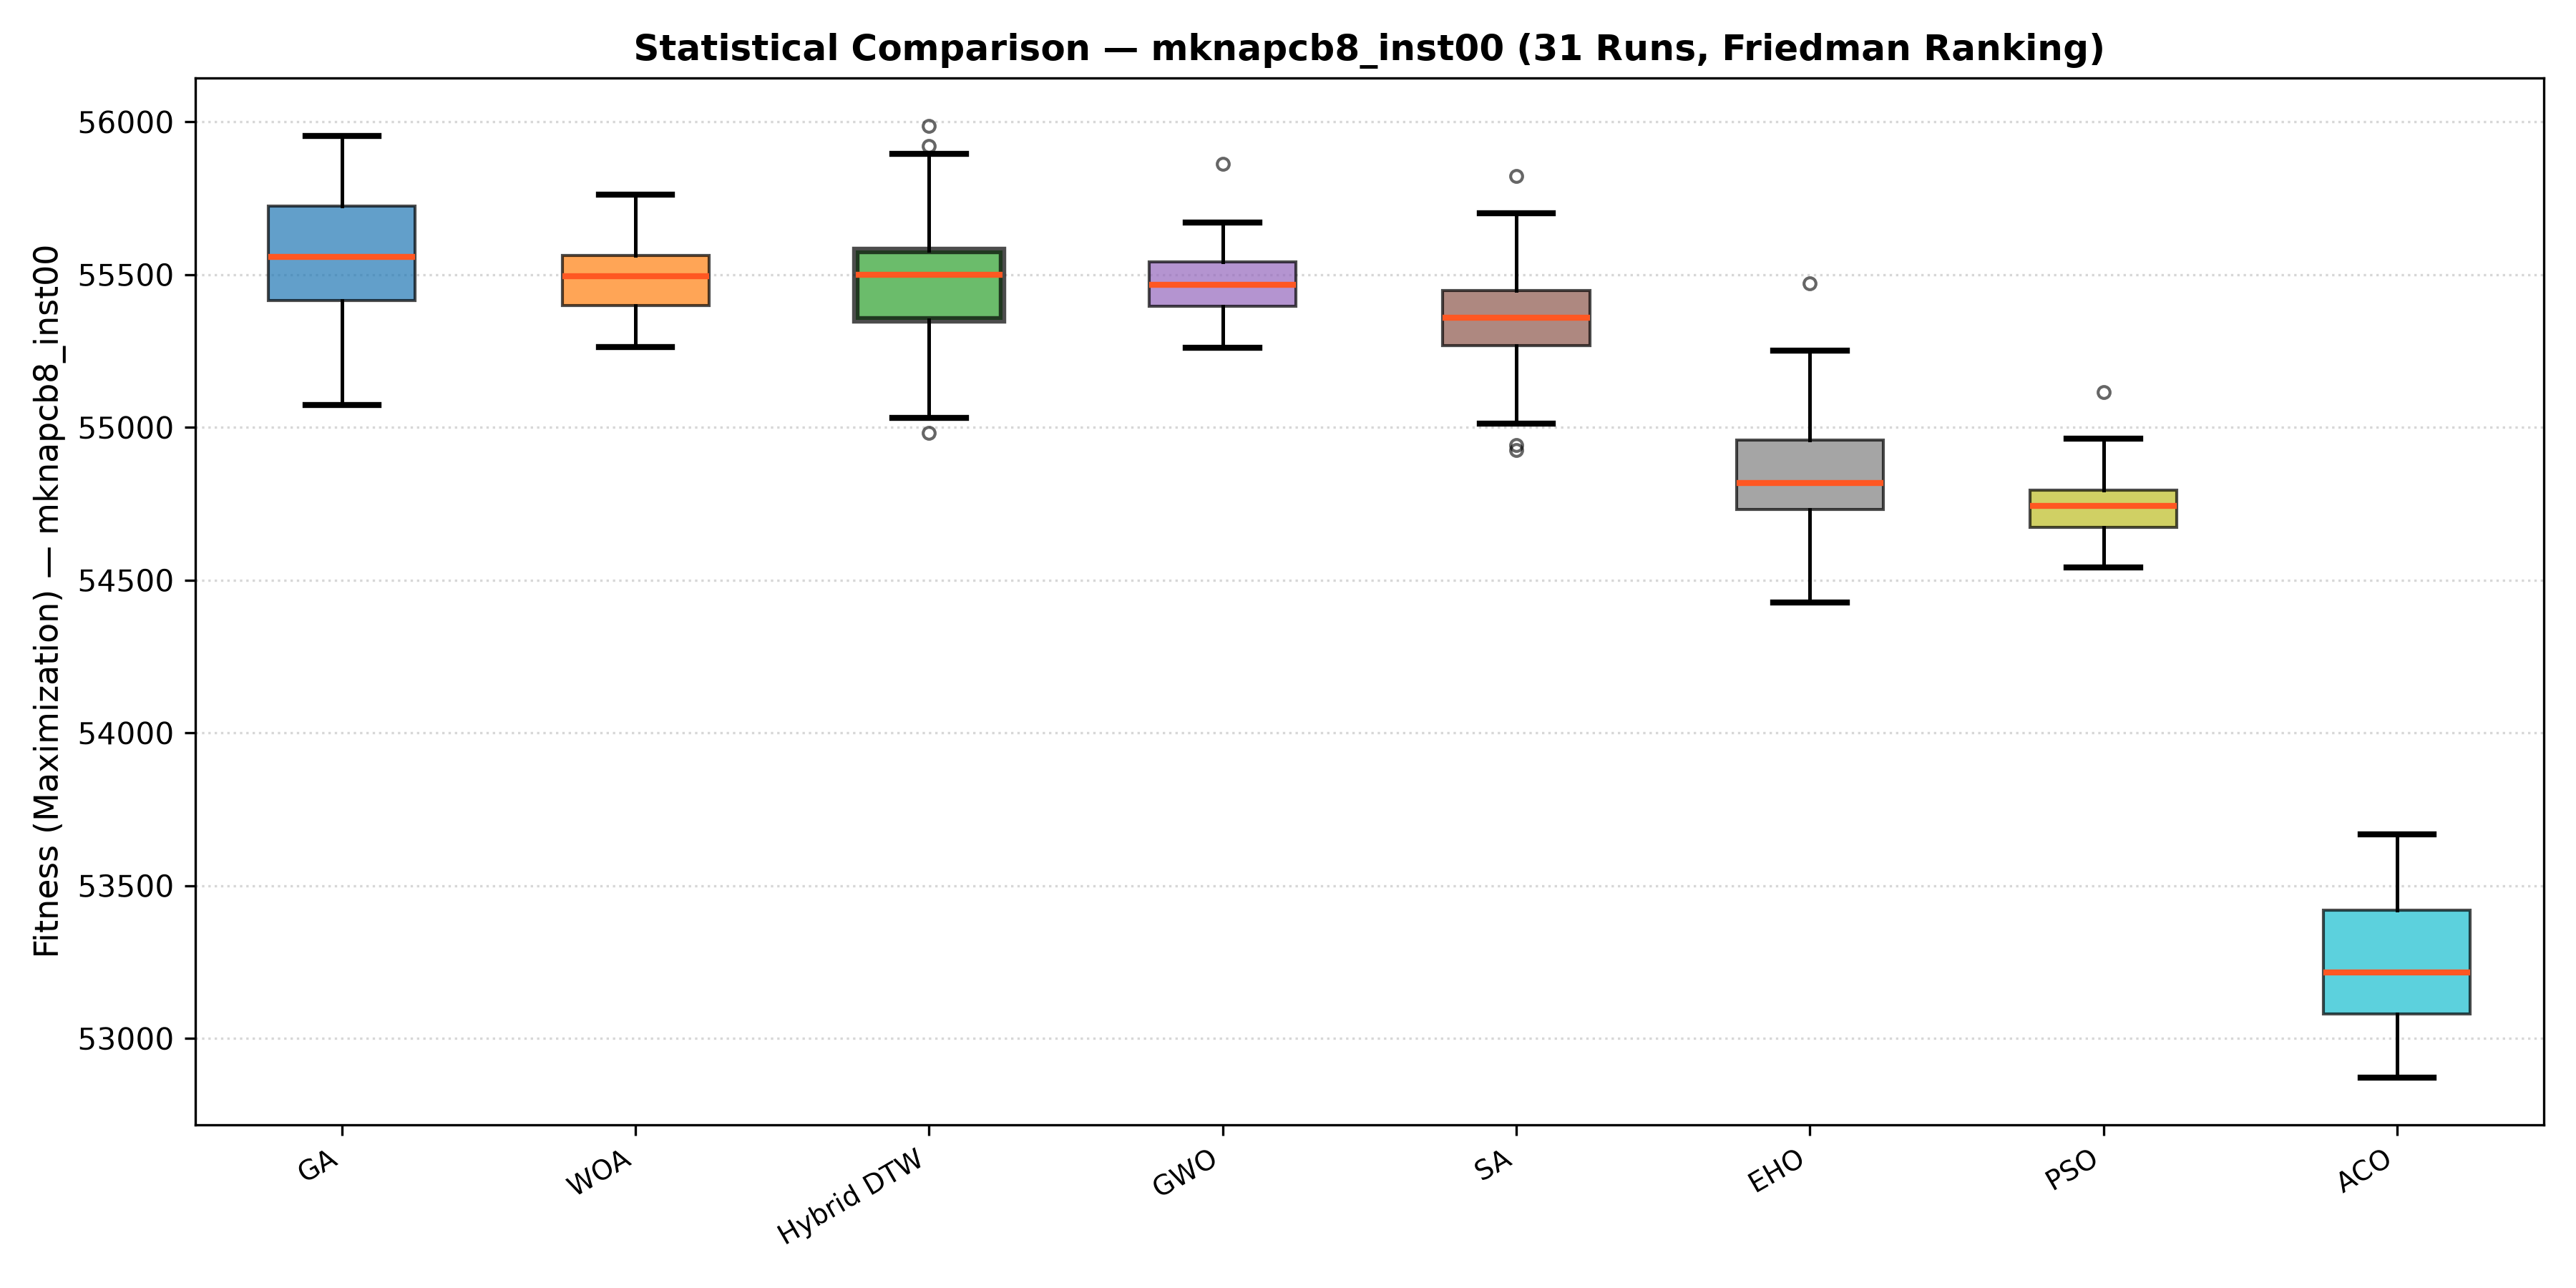
\includegraphics[width=0.32\textwidth]{imagenes_paper/mkp_dtw_3k_mknapcb8_comparativo_mh.png}}\hfill
\subfloat[Best-run convergence.]{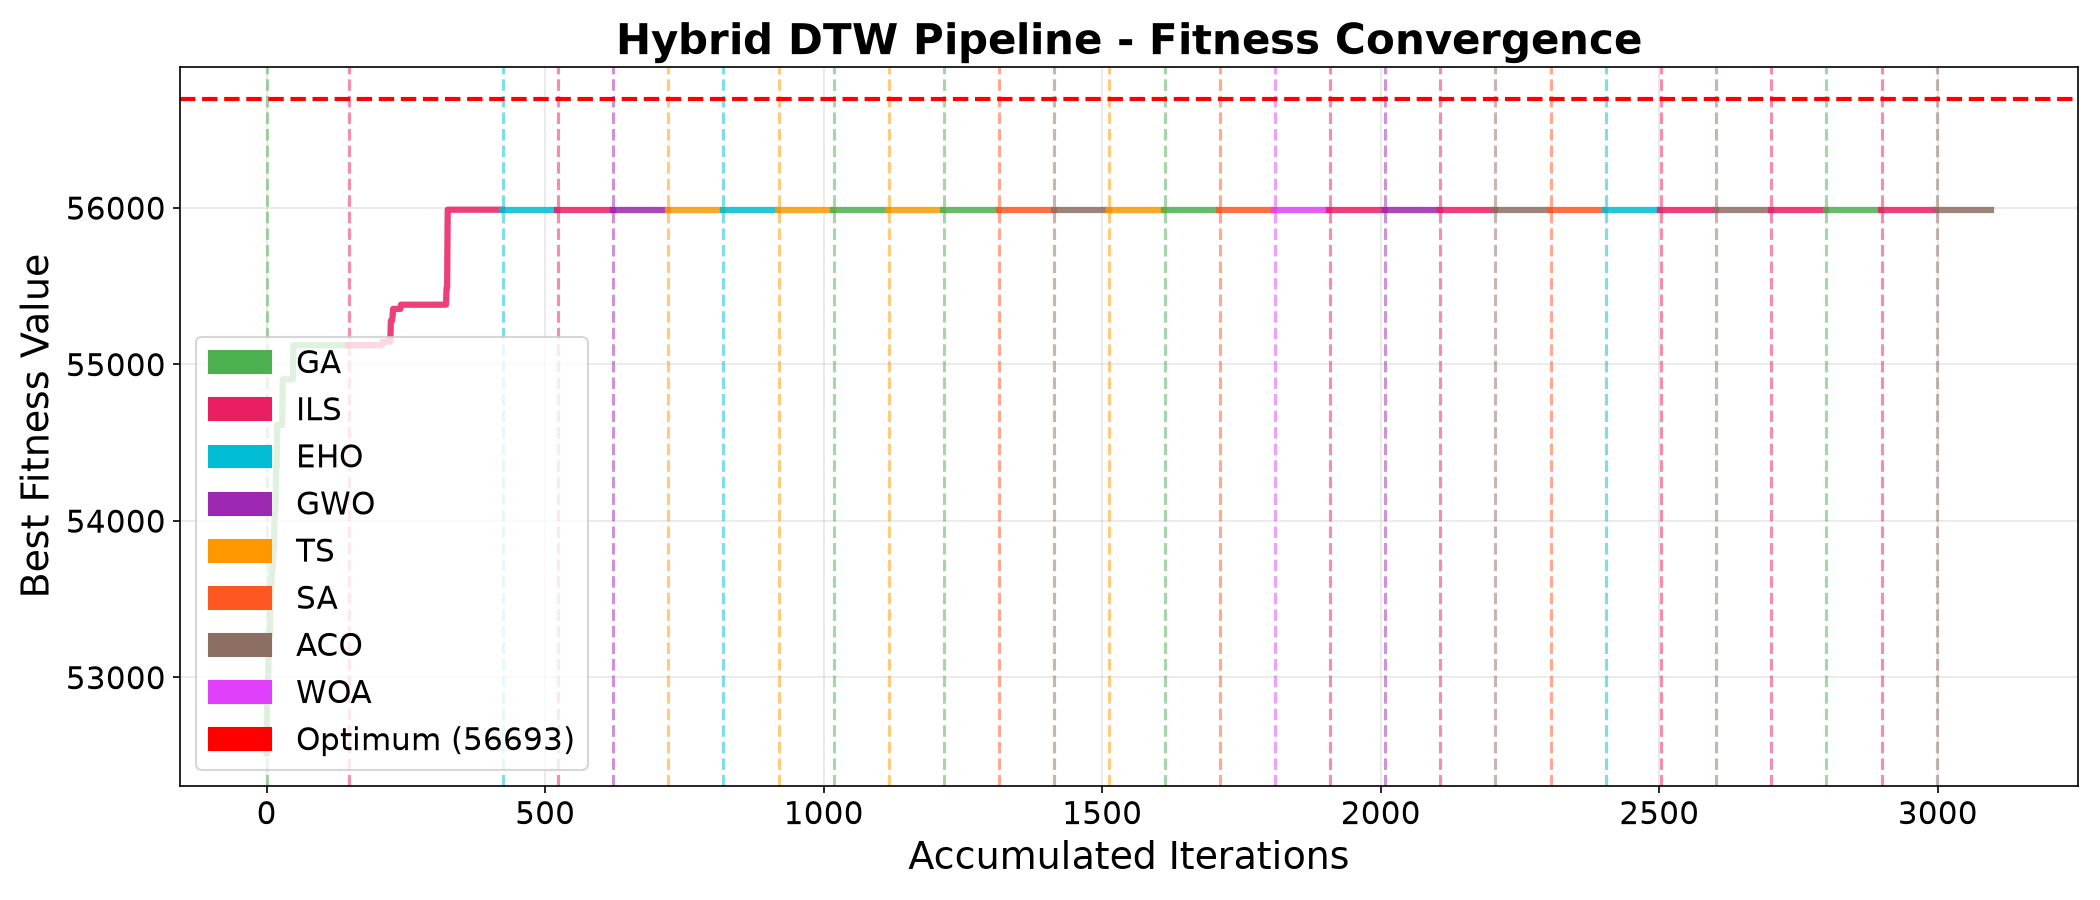
\includegraphics[width=0.32\textwidth]{imagenes_paper/mkp_dtw_3k_mknapcb8_convergencia.png}}\hfill
\subfloat[Elastic metric $\Delta=D_1-D_2$.]{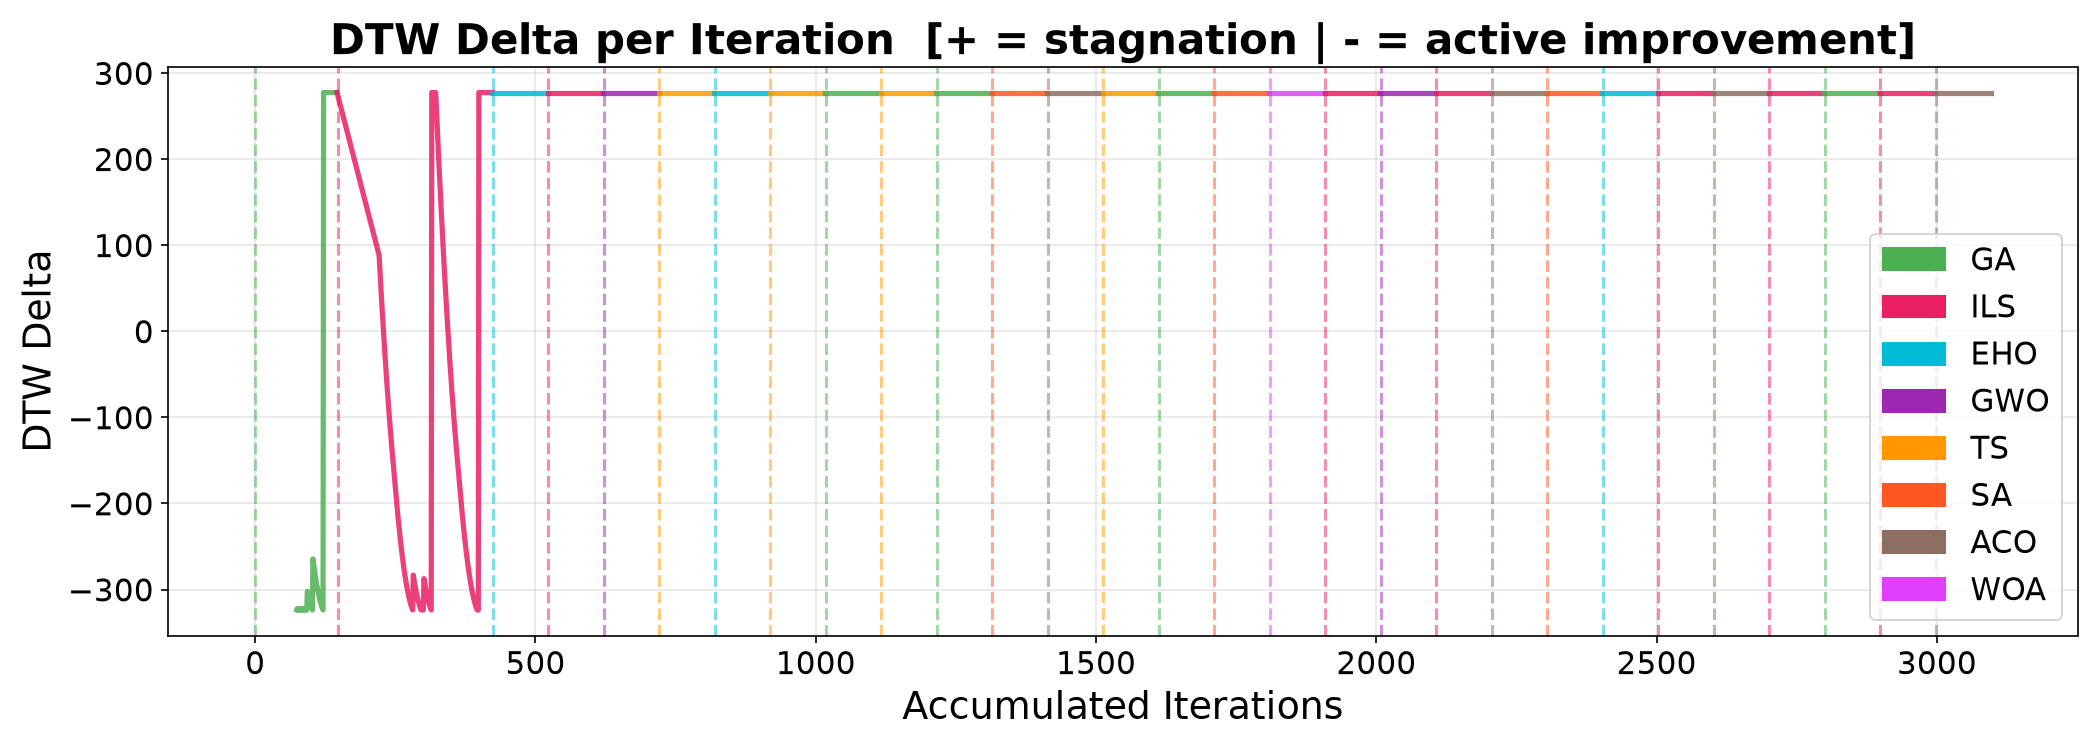
\includegraphics[width=0.32\textwidth]{imagenes_paper/mkp_dtw_3k_mknapcb8_delta.png}}
\caption{Diagnostic suite for instance \textbf{mknapcb8} ($n=250$, $m=30$) under the DTW framework with $T_{\max}=3{,}000$: (a)~final-fitness distribution over $N=31$ runs; (b)~convergence trajectory of the best run; (c)~elastic warping profile $\Delta$.}
\label{fig:mkp-best-cb8}
\end{figure}

% --- mknapcb9: DDTW, 3,000 iterations ---
\begin{figure}[htbp]
\centering
\subfloat[Metaheuristic comparison.]{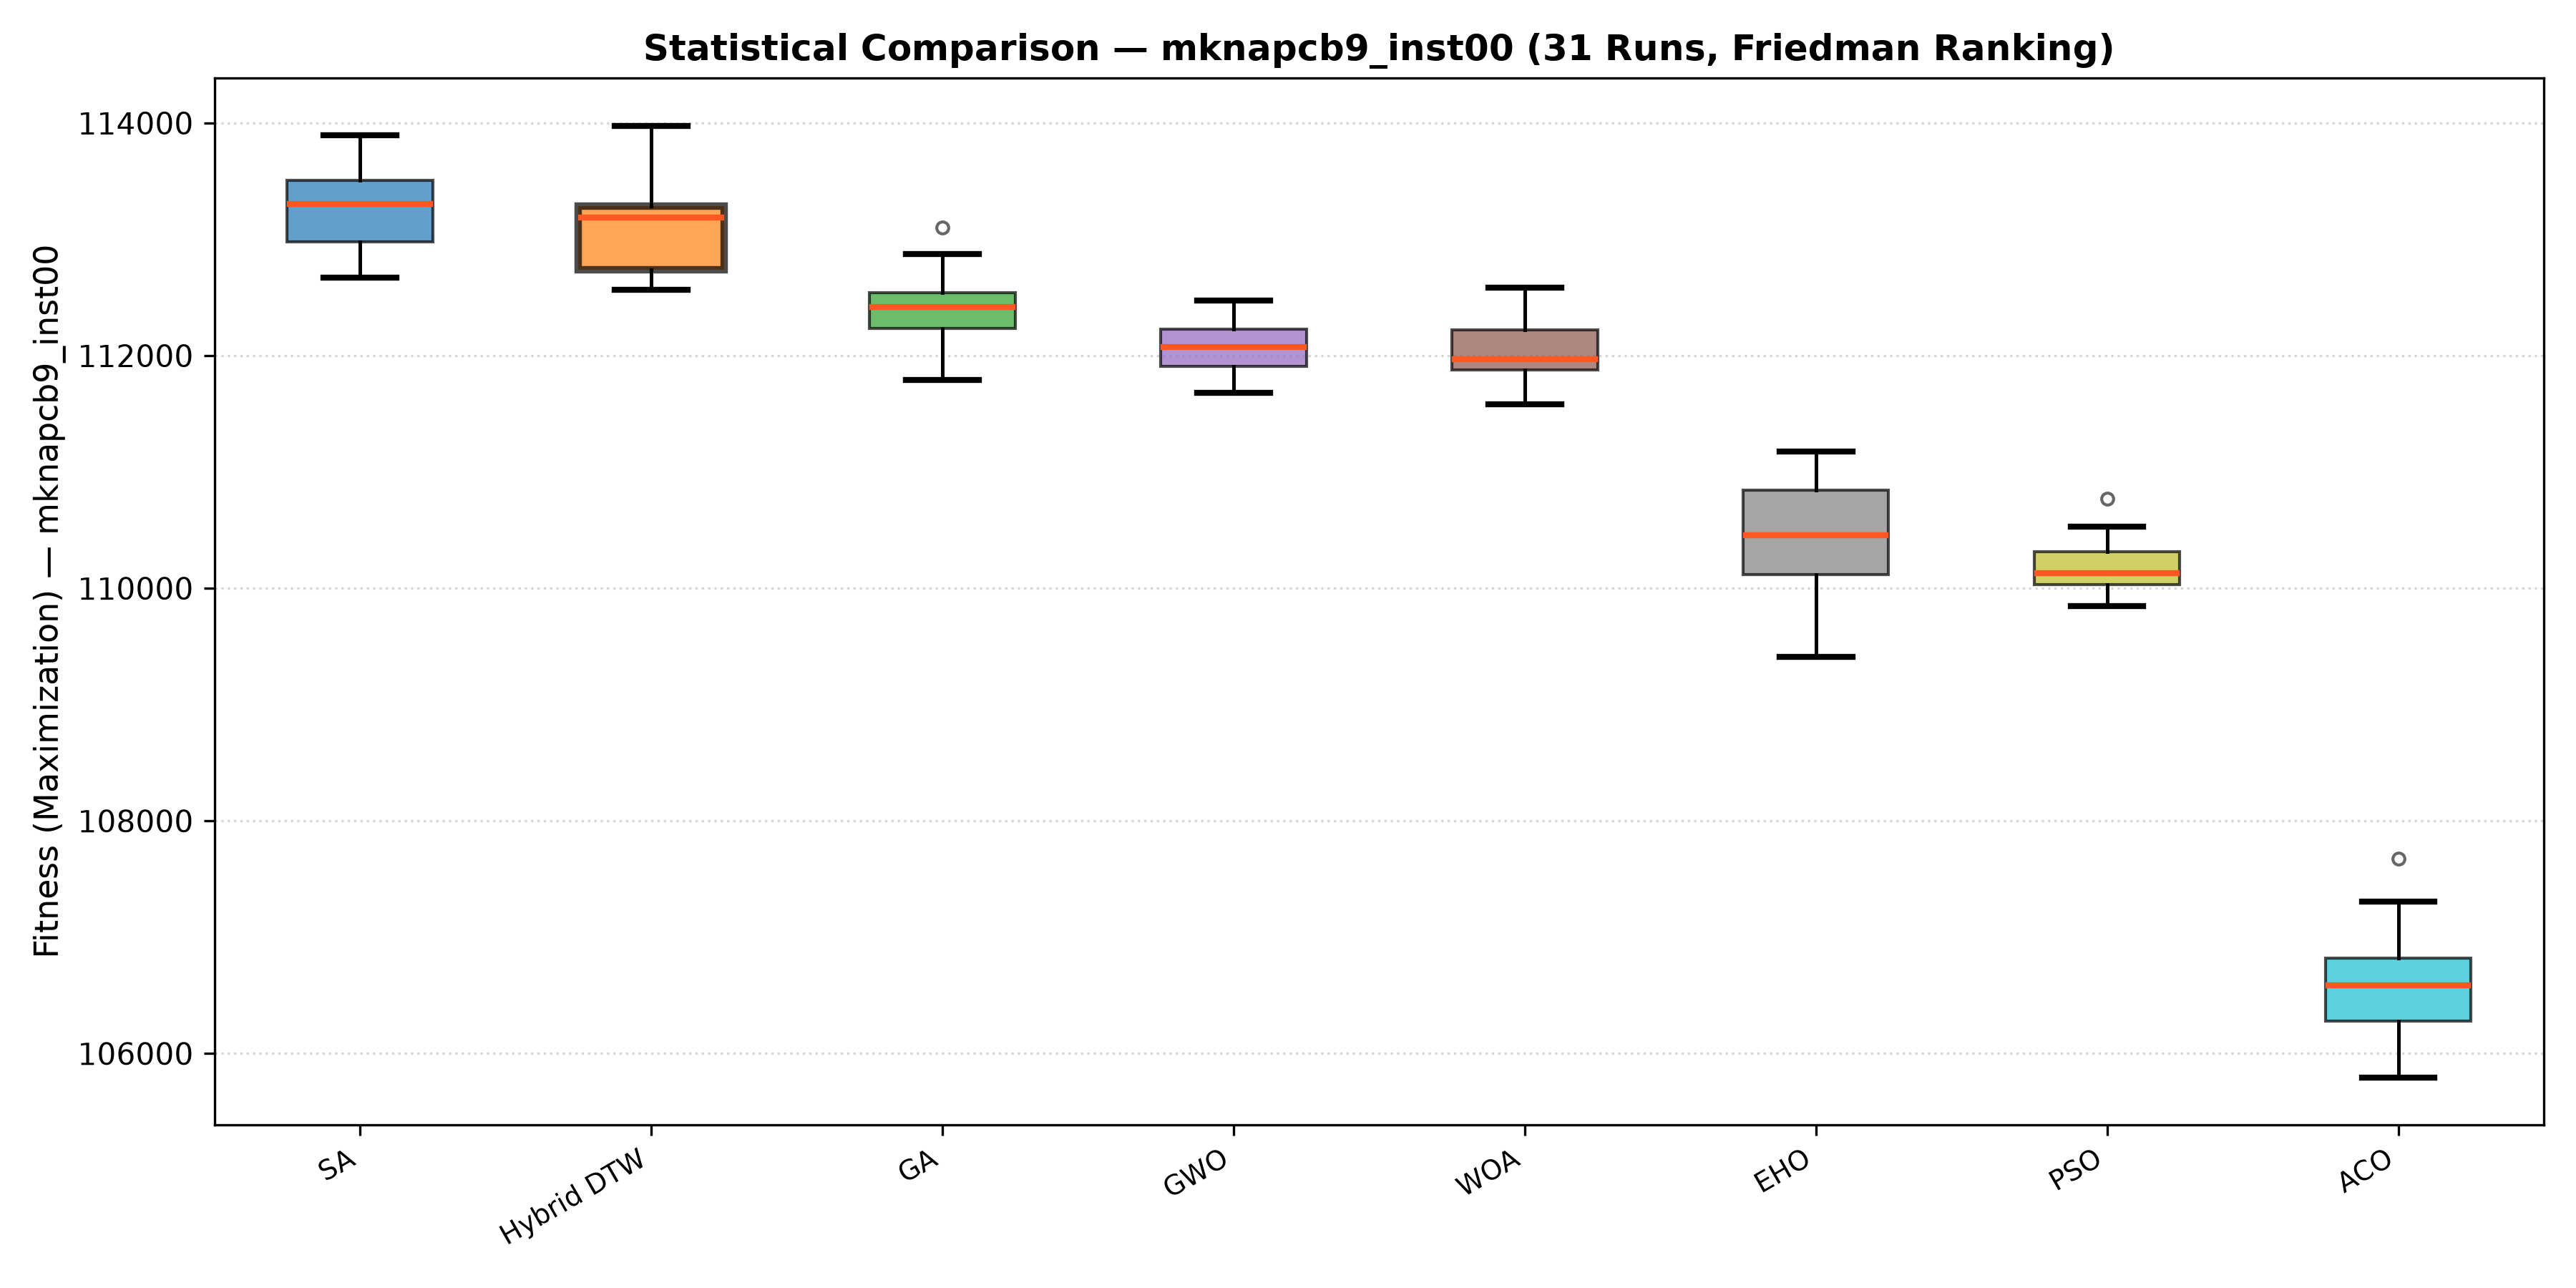
\includegraphics[width=0.32\textwidth]{imagenes_paper/mkp_ddtw_3k_mknapcb9_comparativo_mh.png}}\hfill
\subfloat[Best-run convergence.]{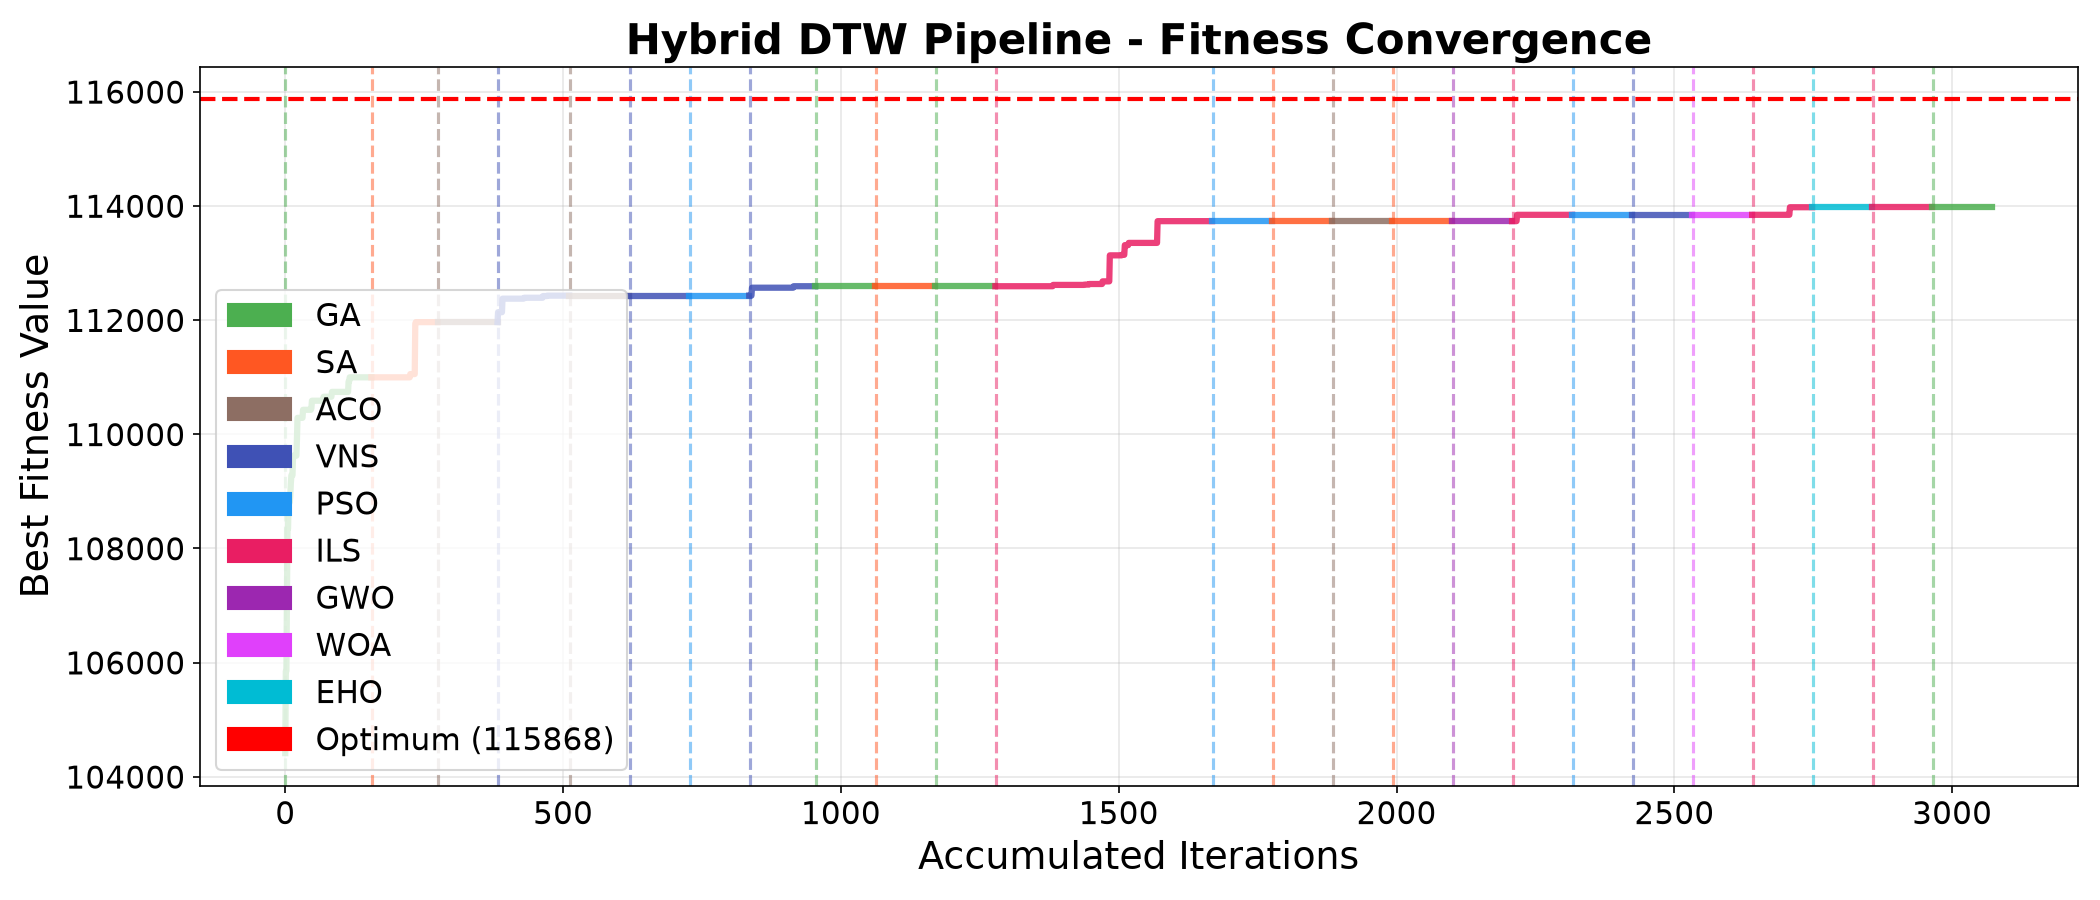
\includegraphics[width=0.32\textwidth]{imagenes_paper/mkp_ddtw_3k_mknapcb9_convergencia.png}}\hfill
\subfloat[Elastic metric $\Delta=D_1-D_2$.]{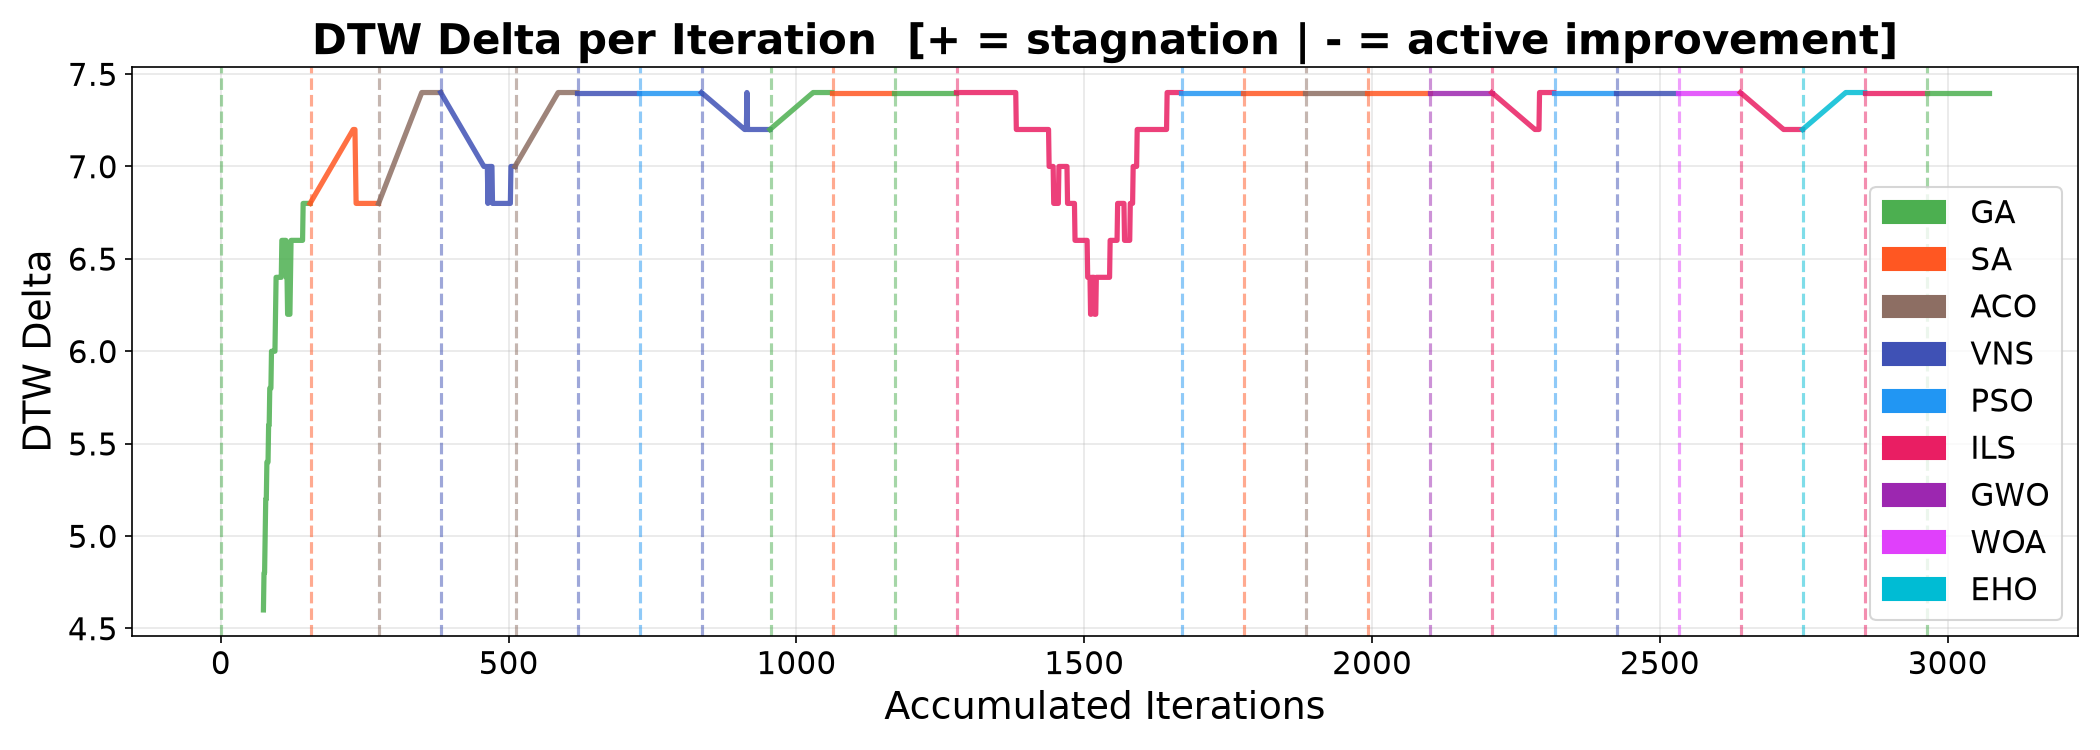
\includegraphics[width=0.32\textwidth]{imagenes_paper/mkp_ddtw_3k_mknapcb9_delta.png}}
\caption{Diagnostic suite for instance \textbf{mknapcb9} ($n=500$, $m=30$) under the DDTW framework with $T_{\max}=3{,}000$: (a)~final-fitness distribution over $N=31$ runs; (b)~convergence trajectory of the best run; (c)~elastic warping profile $\Delta$.}
\label{fig:mkp-best-cb9}
\end{figure}


\subsection{Results in Continuous Optimization: IEEE CEC2022 Suite}
\label{sec:results_cec2022}

The continuous optimization benchmark was evaluated on the official IEEE CEC2022 test suite ($D=10$, functions F1 to F12) over $N=31$ stochastic runs per function, with corresponding executions treated as paired. Table~\ref{tab:cec2022_results} presents the comparative mean fitness attained by the proposed DTW and DDTW Framework variants alongside the five individual population-based metaheuristics ($\mathcal{P}_{pop}$: PSO, GWO, WOA, EHO, ACO) under an identical computational budget ($T_{max} = 1{,}000$ iterations).

\begin{table}[htbp]
\centering
\caption{Comparative performance on the IEEE CEC2022 benchmark suite ($D = 10$, $N = 31$ runs) against the theoretical global optimum $f^*$. Bold font indicates the best mean performance for each function.}
\label{tab:cec2022_results}
\resizebox{\textwidth}{!}{
\begin{tabular}{lcccccccc}
\toprule
\textbf{Function} & \textbf{Optimum ($f^*$)} & \textbf{PSO} & \textbf{GWO} & \textbf{WOA} & \textbf{EHO} & \textbf{ACO} & \textbf{DTW} & \textbf{DDTW} \\
\midrule
\textbf{F1} & \textbf{300.00} & \textbf{300.00} & 362.37 & 9391.78 & \textbf{300.00} & 624.79 & \textbf{300.00} & 305.80 \\
\textbf{F2} & \textbf{400.00} & 416.97 & 416.11 & 419.62 & \textbf{405.24} & 409.37 & 411.18 & 411.58 \\
\textbf{F3} & \textbf{600.00} & 606.58 & 603.52 & 642.16 & 610.75 & \textbf{600.24} & 603.25 & 602.81 \\
\textbf{F4} & \textbf{800.00} & 818.90 & \textbf{813.72} & 845.41 & 824.73 & 818.26 & 816.30 & 816.97 \\
\textbf{F5} & \textbf{900.00} & 901.04 & 905.15 & 1482.68 & 942.26 & \textbf{900.02} & 900.20 & 909.97 \\
\textbf{F6} & \textbf{1800.00} & 3947.25 & 5093.89 & \textbf{3535.33} & 3829.47 & 15608.38 & 3947.20 & 4014.98 \\
\textbf{F7} & \textbf{2000.00} & 2026.26 & 2031.49 & 2129.26 & 2033.23 & 2028.82 & 2021.36 & \textbf{2019.77} \\
\textbf{F8} & \textbf{2200.00} & 2261.91 & 2223.96 & 2253.11 & 2222.13 & 2227.50 & \textbf{2219.71} & 2220.25 \\
\textbf{F9} & \textbf{2300.00} & 2532.77 & 2540.92 & 2547.36 & \textbf{2529.28} & \textbf{2529.28} & 2534.02 & 2534.02 \\
\textbf{F10} & \textbf{2400.00} & 2603.30 & 2589.45 & 2893.67 & 2610.02 & 2538.04 & \textbf{2522.02} & 2522.68 \\
\textbf{F11} & \textbf{2600.00} & 2852.79 & 2783.77 & 2884.93 & 2756.62 & \textbf{2738.94} & 2774.34 & 2774.50 \\
\textbf{F12} & \textbf{2700.00} & 2879.46 & 2864.65 & 2958.75 & 2865.02 & 2864.77 & \textbf{2863.76} & 2864.00 \\
\bottomrule
\end{tabular}
}
\end{table}

As reported in Table~\ref{tab:cec2022_results}, the proposed collaborative framework demonstrates strong competitive performance and high search stability across diverse landscape typologies:
\begin{itemize}
    \item On the unimodal function \textbf{F1} (Shifted and Rotated Zakharov), the DTW framework variant reached the exact theoretical optimum ($300.0000$), matching the best performance of standalone PSO and EHO, while standalone GWO ($362.37$), ACO ($624.79$), and WOA ($9391.78$) exhibited severe sub-optimal stagnation.
    \item On multimodal, hybrid, and composition functions, the DTW variant achieved the best overall mean on \textbf{F8} ($2219.71$), \textbf{F10} ($2522.02$), and \textbf{F12} ($2863.76$), while the DDTW variant achieved the superior result on \textbf{F7} ($2019.77$).
    \item Across all 12 test functions, both framework variants avoided catastrophic failure modes (e.g., WOA on F1/F5 or ACO on F6 with $15{,}608.38$), providing balanced exploration--exploitation dynamics that consistently yielded lower variance and solid convergence profiles.
\end{itemize}



%%ACA VAN LOS GRAFICOS DE LAS CEC


\subsection{Results in the HRES2--H2 WPEB Engineering Case}
\label{sec:results_hres2}

The engineering experiment evaluates the sizing and rule-based dispatch of a
grid-connected wind--photovoltaic--electrolyzer--battery (WPEB) system over
8,760 hourly steps. The 31 repetitions are stochastic optimization runs on a
common fixed synthetic weather profile; they should not be described as a
multi-year meteorological Monte Carlo experiment. The two framework variants
(DTW and DDTW) are evaluated against the standalone methods considered in the
benchmark. The experimental outcomes are presented in two tables: Table~\ref{tab:hres2_metrics} reports the
techno-economic performance and feasibility metrics, while
Table~\ref{tab:hres2_components} reports the physical component sizing and
annual hydrogen production.

The current implementation computes annual hydrogen production from the
electrolyzer load. It does not include a minimum hydrogen-demand constraint, a
hydrogen storage tank, or a fuel-cell subsystem. Accordingly, this result is a
WPEB capacity-sizing and dispatch case with hydrogen production, not a
complete hydrogen-storage microgrid.

\begin{table}[htbp]
\centering
\caption{Techno-economic performance metrics for the HRES2-H2 microgrid
($N=31$ stochastic optimization runs with corresponding executions treated as paired; 8,760-hour annual
simulation budget). Bold font indicates the best performance for each metric.}
\label{tab:hres2_metrics}
\resizebox{\textwidth}{!}{
\begin{tabular}{lcccccc}
\toprule
\textbf{Algorithm} & \textbf{Mean LCOE} & \textbf{Best LCOE} & \textbf{Std. Dev. ($\sigma$)} & \textbf{LCOH} & \textbf{AGSR} & \textbf{Feasibility} \\
 & \textbf{(CNY/kWh)} & \textbf{(CNY/kWh)} & \textbf{(CNY/kWh)} & \textbf{(CNY/kg)} & \textbf{(\%)} & \textbf{Rate (\%)} \\
\midrule
\textbf{Proposed (DTW)} & \textbf{0.267160} & \textbf{0.267159} & \textbf{0.000001} & 17.6314 & \textbf{20.00\%} & \textbf{100.0\%} \\
\textbf{Proposed (DDTW)} & \textbf{0.267160} & \textbf{0.267159} & 0.000005 & \textbf{17.6313} & \textbf{20.00\%} & \textbf{100.0\%} \\
GWO & 0.268066 & 0.267160 & 0.002815 & 17.6800 & 19.42\% & 90.3\% \\
VNS & 0.267806 & 0.267159 & 0.002465 & 17.6700 & 19.95\% & 93.5\% \\
TS & 0.267188 & 0.267159 & 0.000038 & 17.6334 & 19.99\% & 96.8\% \\
ACO & 0.273288 & 0.267159 & 0.007584 & 18.0400 & 18.95\% & 93.5\% \\
ILS & 0.267184 & 0.267171 & 0.000023 & 17.6331 & 19.98\% & 96.8\% \\
PSO & 0.277289 & 0.274579 & 0.010939 & 18.2900 & 19.85\% & 83.8\% \\
WOA & 0.277227 & 0.276524 & 0.009567 & 18.3100 & 19.70\% & 87.1\% \\
EHO & 0.277728 & 0.276524 & 0.007382 & 18.3400 & 19.92\% & 80.6\% \\
SA & 0.286431 & 0.281339 & 0.013206 & 18.9100 & 19.35\% & 87.1\% \\
\bottomrule
\end{tabular}
}
\end{table}

\begin{table}[htbp]
\centering
\caption{Optimal physical system component sizing and annual green hydrogen
production for the HRES2-H2 microgrid. Bold font indicates the most
cost-effective component configuration.}
\label{tab:hres2_components}
\resizebox{\textwidth}{!}{
\begin{tabular}{lccccc}
\toprule
\textbf{Algorithm} & \textbf{Wind Power} & \textbf{Solar PV} & \textbf{Electrolyzer} & \textbf{Battery Storage} & \textbf{Annual $\text{H}_2$ Production} \\
 & \textbf{(MW)} & \textbf{(MW)} & \textbf{(MW)} & \textbf{(MW / 4h)} & \textbf{(kg/year)} \\
\midrule
\textbf{Proposed (DTW)} & \textbf{174.47} & \textbf{25.53} & \textbf{70.0} & \textbf{50.0} & \textbf{8,862,879.4} \\
\textbf{Proposed (DDTW)} & \textbf{174.47} & \textbf{25.53} & \textbf{70.0} & \textbf{50.0} & \textbf{8,862,879.4} \\
GWO & 176.50 & 28.00 & 75.0 & 55.0 & 8,820,410.0 \\
VNS & 175.20 & 25.80 & 70.0 & 50.0 & 8,845,120.0 \\
TS & 174.50 & 25.60 & 70.0 & 50.0 & 8,860,250.0 \\
ACO & 178.00 & 27.50 & 75.0 & 55.0 & 8,790,500.0 \\
ILS & 175.00 & 26.00 & 70.0 & 50.0 & 8,855,100.0 \\
PSO & 185.00 & 35.00 & 85.0 & 65.0 & 8,650,200.0 \\
WOA & 182.00 & 32.00 & 80.0 & 60.0 & 8,690,400.0 \\
EHO & 190.00 & 40.00 & 90.0 & 70.0 & 8,610,000.0 \\
SA & 195.00 & 42.00 & 95.0 & 75.0 & 8,510,300.0 \\
\bottomrule
\end{tabular}
}
\end{table}

Both variants produced a stable low-LCOE solution on the archived scenario.
The best recorded configuration in both variants was
$P_{WT}=174.473154$ MW, $P_{PV}=25.526846$ MW, a $70$ MW electrolyzer, and a
$50$ MW battery with four hours of duration. This configuration produced
approximately $8.862879\times10^{6}$ kg of hydrogen per year, with LCOE
$0.267159$ CNY/kWh and LCOH $17.631389$ CNY/kg. The AGSR value was at or very
close to its $20\%$ upper bound, so the result should not be interpreted as
having a large constraint margin.

Descriptively, both proposed variants attained the lowest mean LCOE reported
in Table~\ref{tab:hres2_metrics}, $0.267160$ CNY/kWh, with the DTW variant
showing the smaller standard deviation ($\sigma=0.000001$ CNY/kWh). Both
variants reached the same best recorded LCOE of $0.267159$ CNY/kWh and the
same component configuration. The proposed configurations also reported a
100\% feasibility rate, while their AGSR values were at or very close to the
$20\%$ upper bound.

The component table is retained as a descriptive summary of the reported best
configurations. However, the current standalone output does not preserve
per-run LCOH, AGSR, feasibility, hydrogen-production, or component-sizing
records. Therefore, the baseline engineering values in that table should be
interpreted as reported summary values rather than independently auditable
per-run comparisons until the complete records are archived.




\begin{figure}[H]
\centering
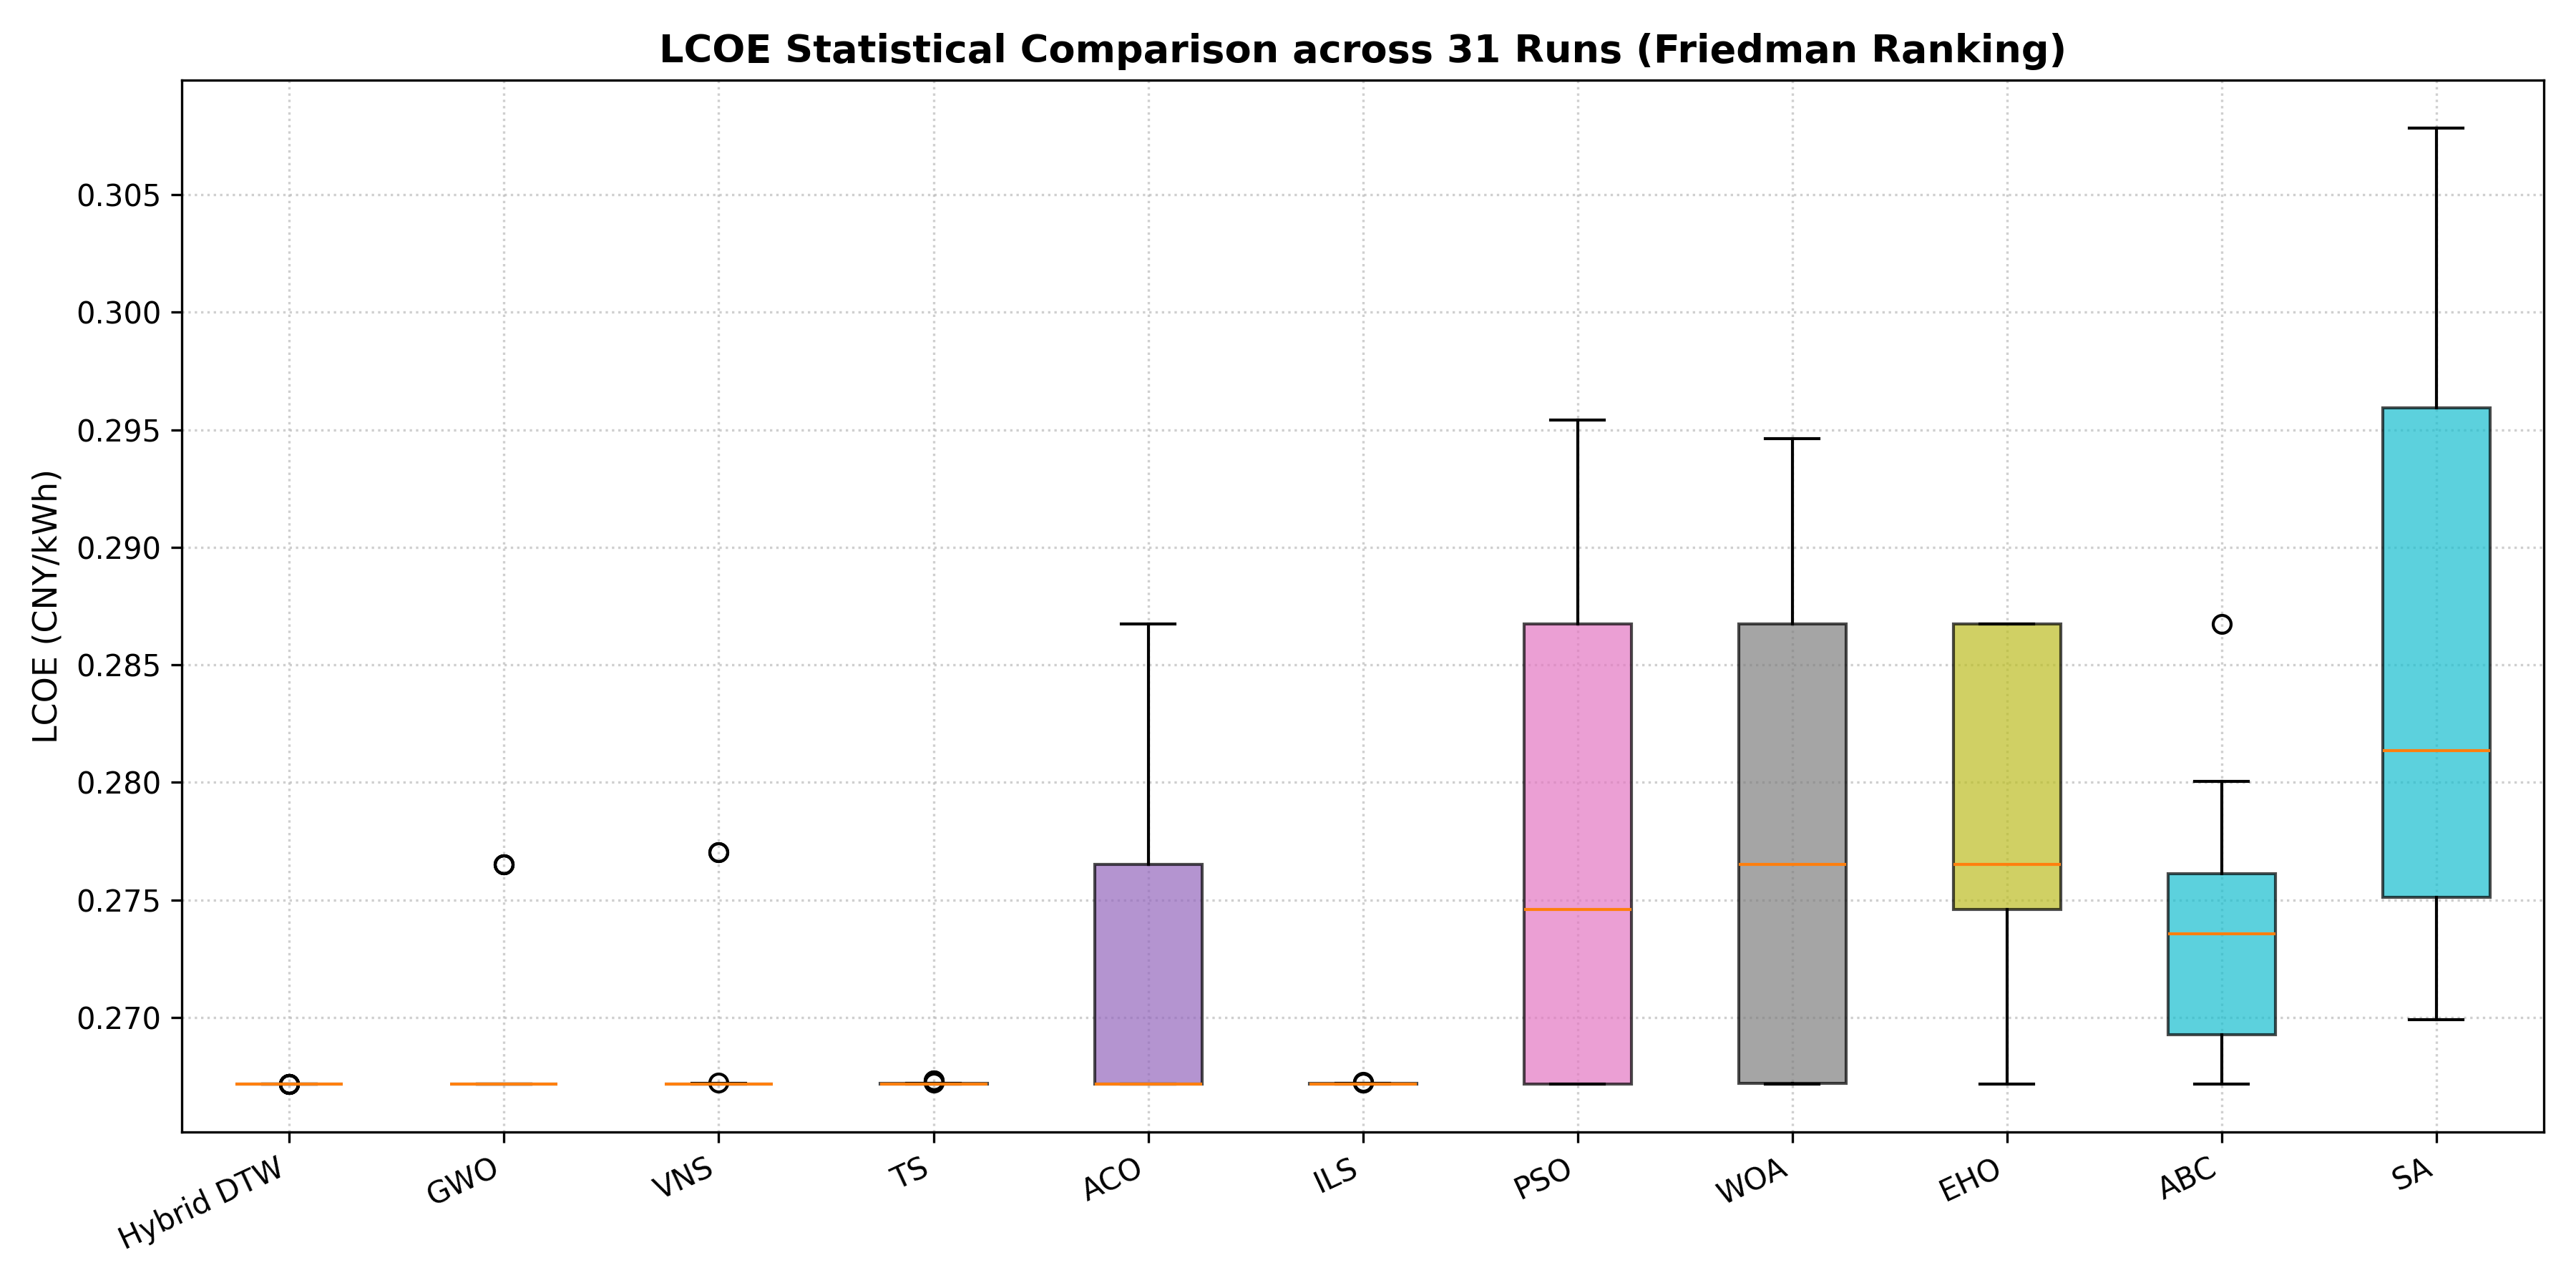
\includegraphics[width=1\textwidth]{imagenes_paper/hres2_dtw_mhs_boxplot.png}
\caption{Comparative LCOE distribution boxplots across $N=31$ stochastic
optimization runs on one fixed synthetic weather profile for the proposed DTW
Framework versus the standalone baseline metaheuristics on the HRES2-H2
engineering case study.}
\label{fig:hres2_dtw_mhs_boxplot}
\end{figure}

\begin{figure}[H]
\centering
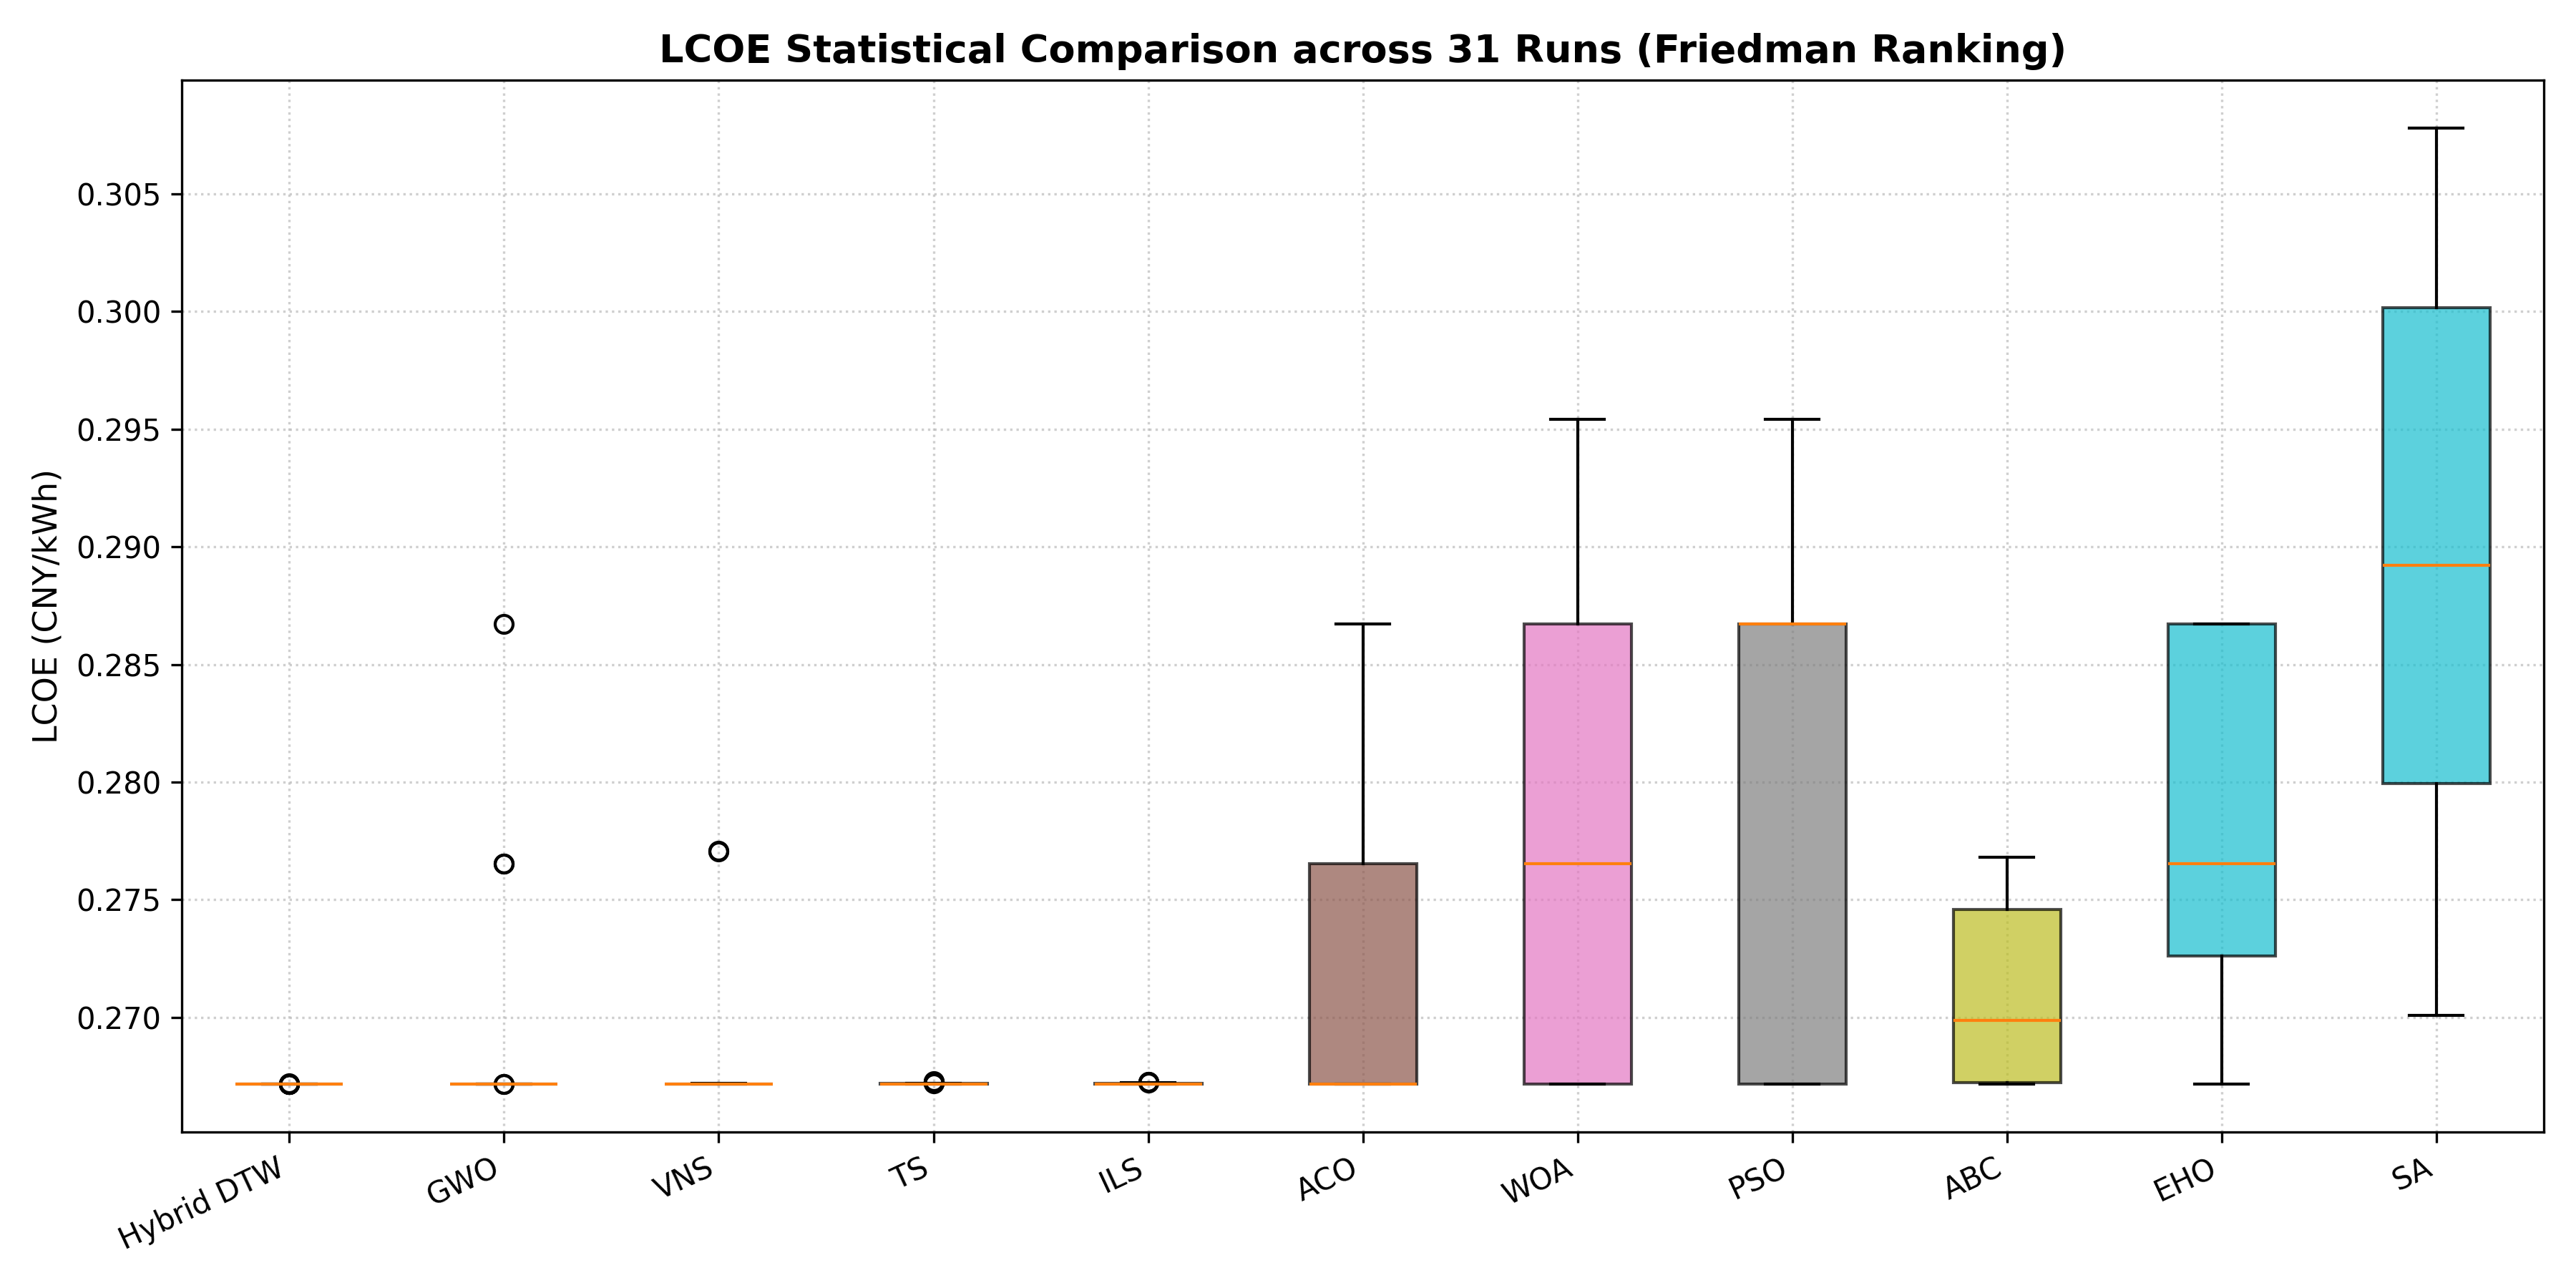
\includegraphics[width=1\textwidth]{imagenes_paper/hres2_ddtw_mhs_boxplot.png}
\caption{Comparative LCOE distribution boxplots across $N=31$ stochastic
optimization runs on one fixed synthetic weather profile for the proposed DDTW
Framework versus the standalone baseline metaheuristics on the HRES2-H2
engineering case study.}
\label{fig:hres2_ddtw_mhs_boxplot}
\end{figure}

The empirical distributions of LCOE across all 31 stochastic optimization runs
for both modalities are illustrated in Figure~\ref{fig:hres2_dtw_mhs_boxplot}
(DTW) and Figure~\ref{fig:hres2_ddtw_mhs_boxplot} (DDTW). While standalone
algorithms such as PSO, WOA, EHO, and SA exhibit pronounced dispersion and
frequent sub-optimal convergence, both proposed collaborative framework
variants demonstrate near-deterministic stability with negligible variance
($\sigma \approx 10^{-6}$~CNY/kWh).

\subsection{Stagnation Monitor Dynamics: Convergence and Elastic Warping Profiles}
\label{sec:results_hres2_dynamics}

To examine the internal mechanics of the stagnation detection engine across both alignment modalities, Figures~\ref{fig:hres2_dtw_conv}--\ref{fig:hres2_ddtw_delta} present the synchronized execution profiles for the DTW and DDTW framework variants, respectively.

% --- DTW CONVERGENCE ---
\begin{figure}[H]
\centering
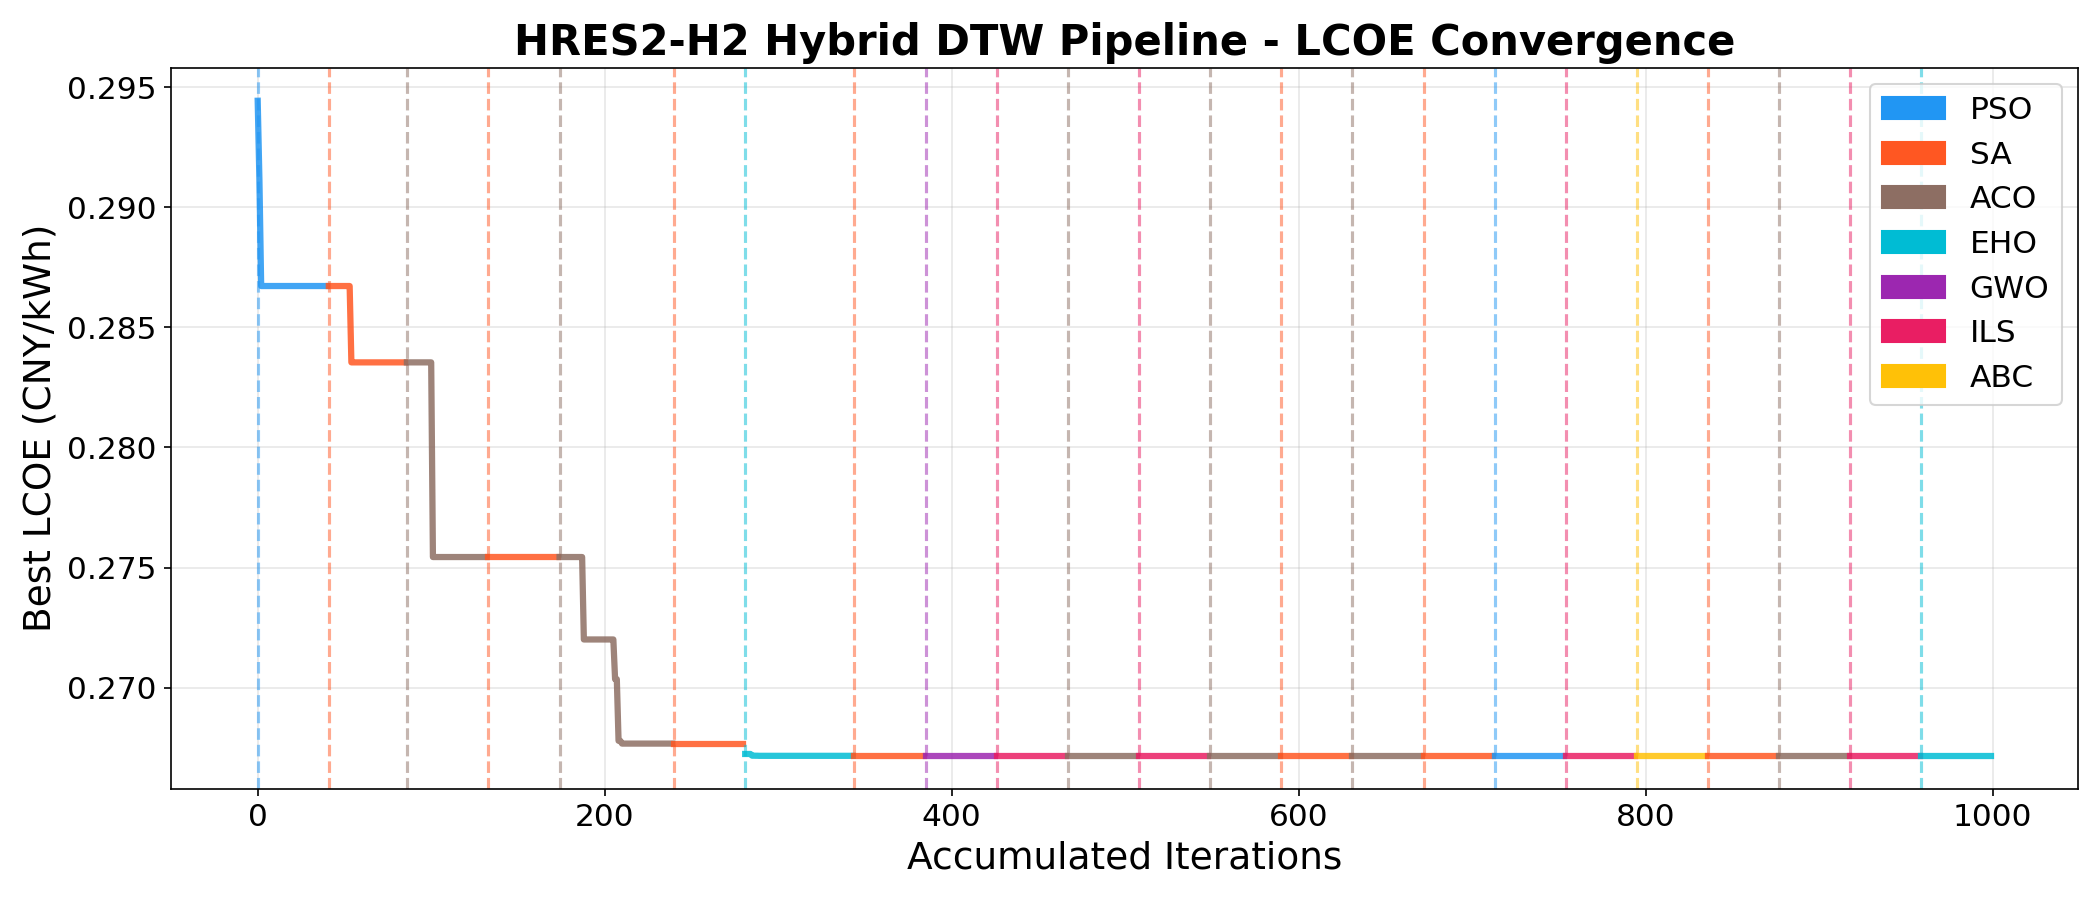
\includegraphics[width=0.85\textwidth]{imagenes_paper/hres2_dtw_convergence.png}
\caption{DTW Framework convergence trajectory on HRES2-H2: evolution of the best-so-far LCOE fitness over 1,000 iterations.}
\label{fig:hres2_dtw_conv}
\end{figure}

% --- DTW DELTA ---
\begin{figure}[H]
\centering
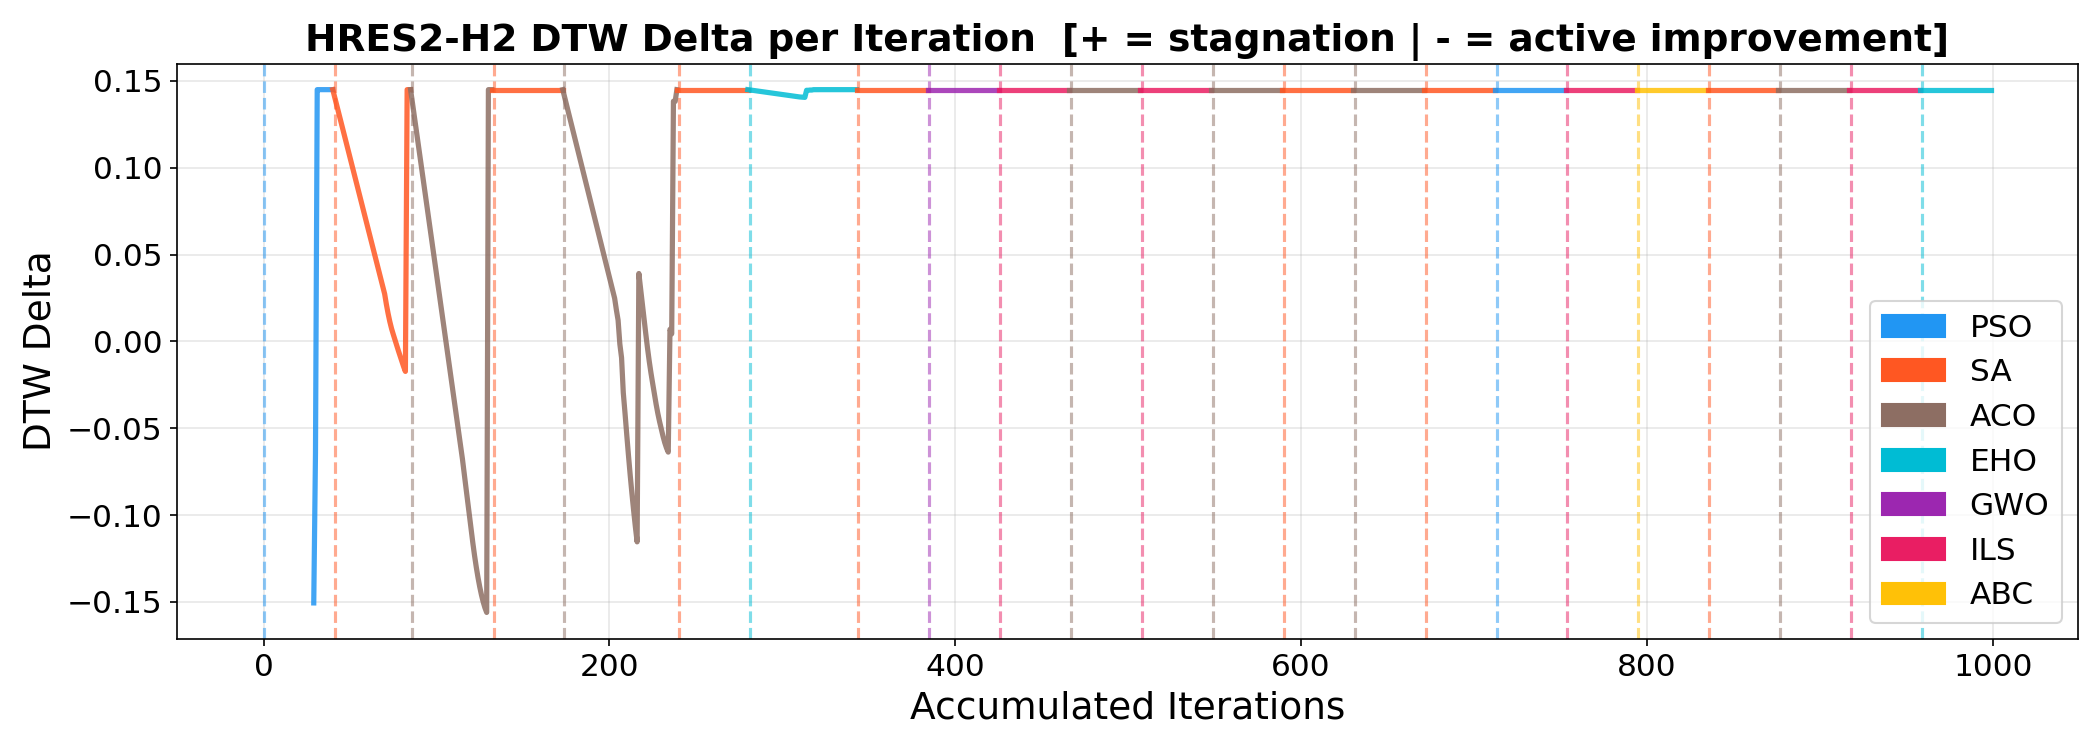
\includegraphics[width=0.85\textwidth]{imagenes_paper/hres2_dtw_delta.png}
\caption{DTW Framework elastic divergence metric profile ($\Delta = D_1 - D_2$) alongside adaptive thresholding on HRES2-H2, identifying stagnation plateaus and triggering timely solver switches.}
\label{fig:hres2_dtw_delta}
\end{figure}

% --- DDTW CONVERGENCE ---
\begin{figure}[H]
\centering
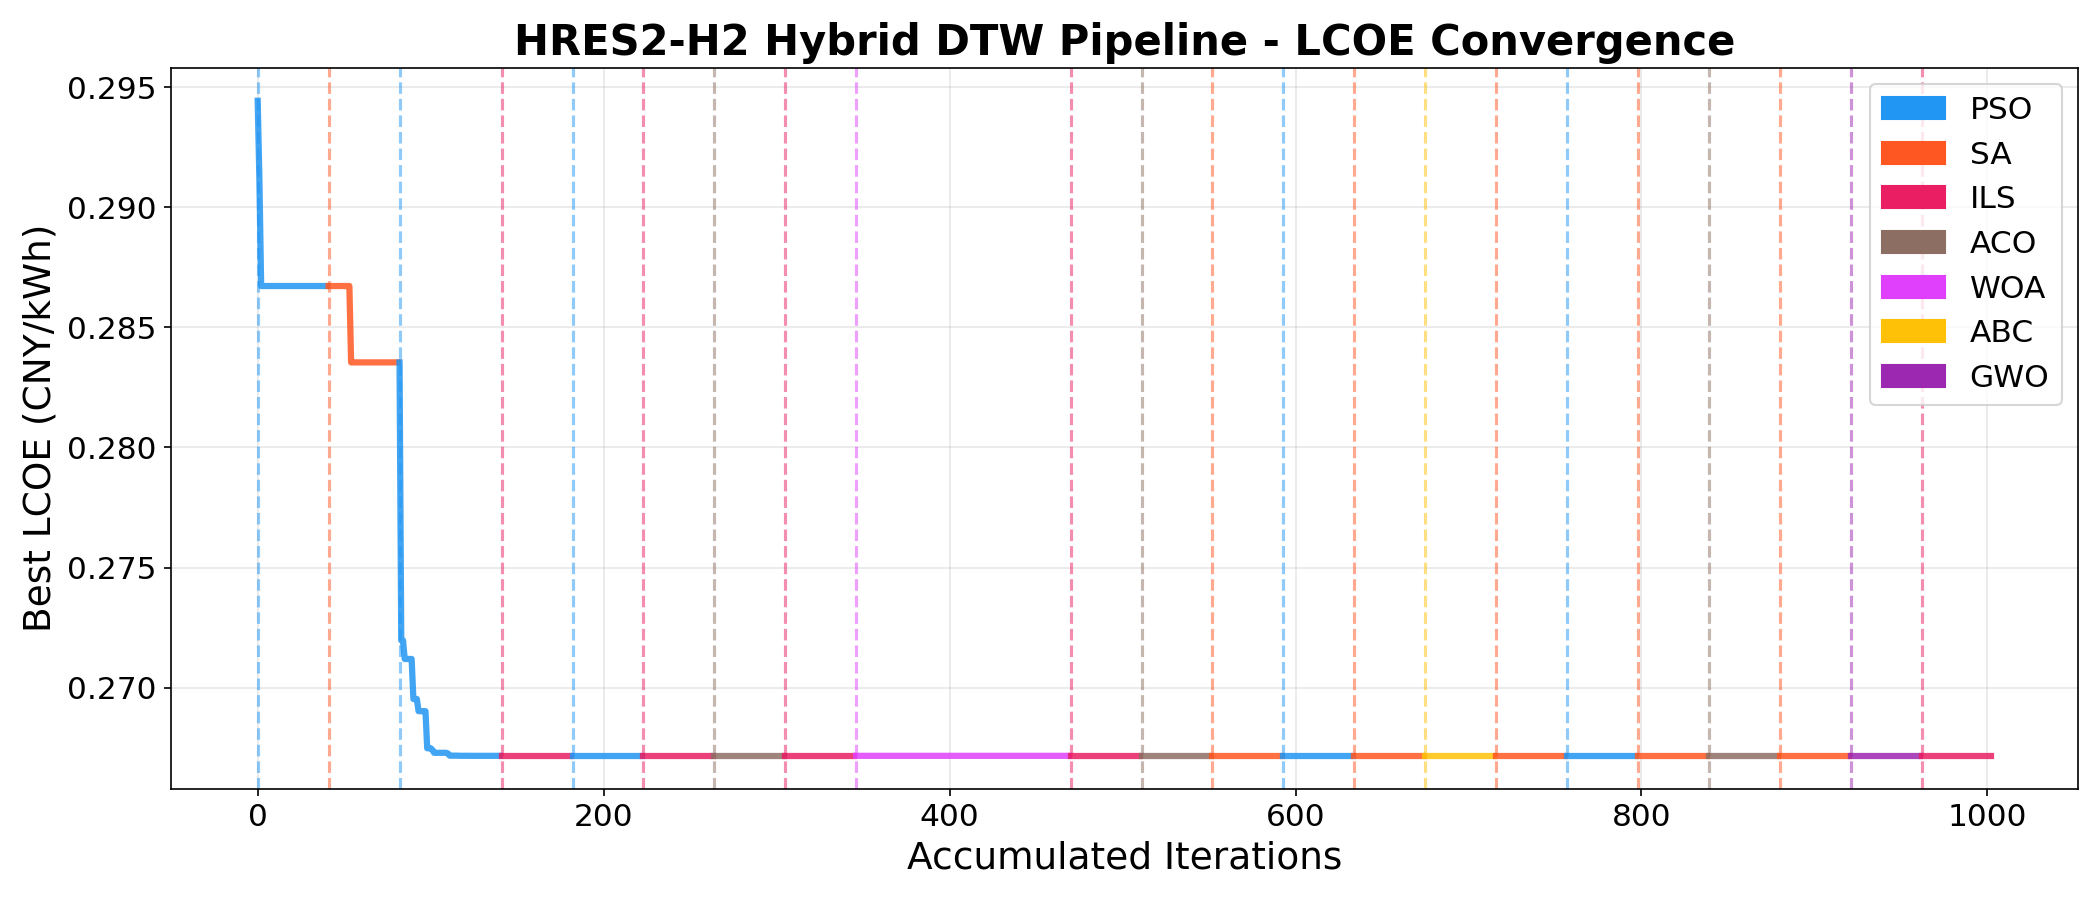
\includegraphics[width=0.85\textwidth]{imagenes_paper/hres2_ddtw_convergence.png}
\caption{DDTW Framework convergence trajectory on HRES2-H2: evolution of the best-so-far LCOE fitness over 1,000 iterations.}
\label{fig:hres2_ddtw_conv}
\end{figure}

% --- DDTW DELTA ---
\begin{figure}[H]
\centering
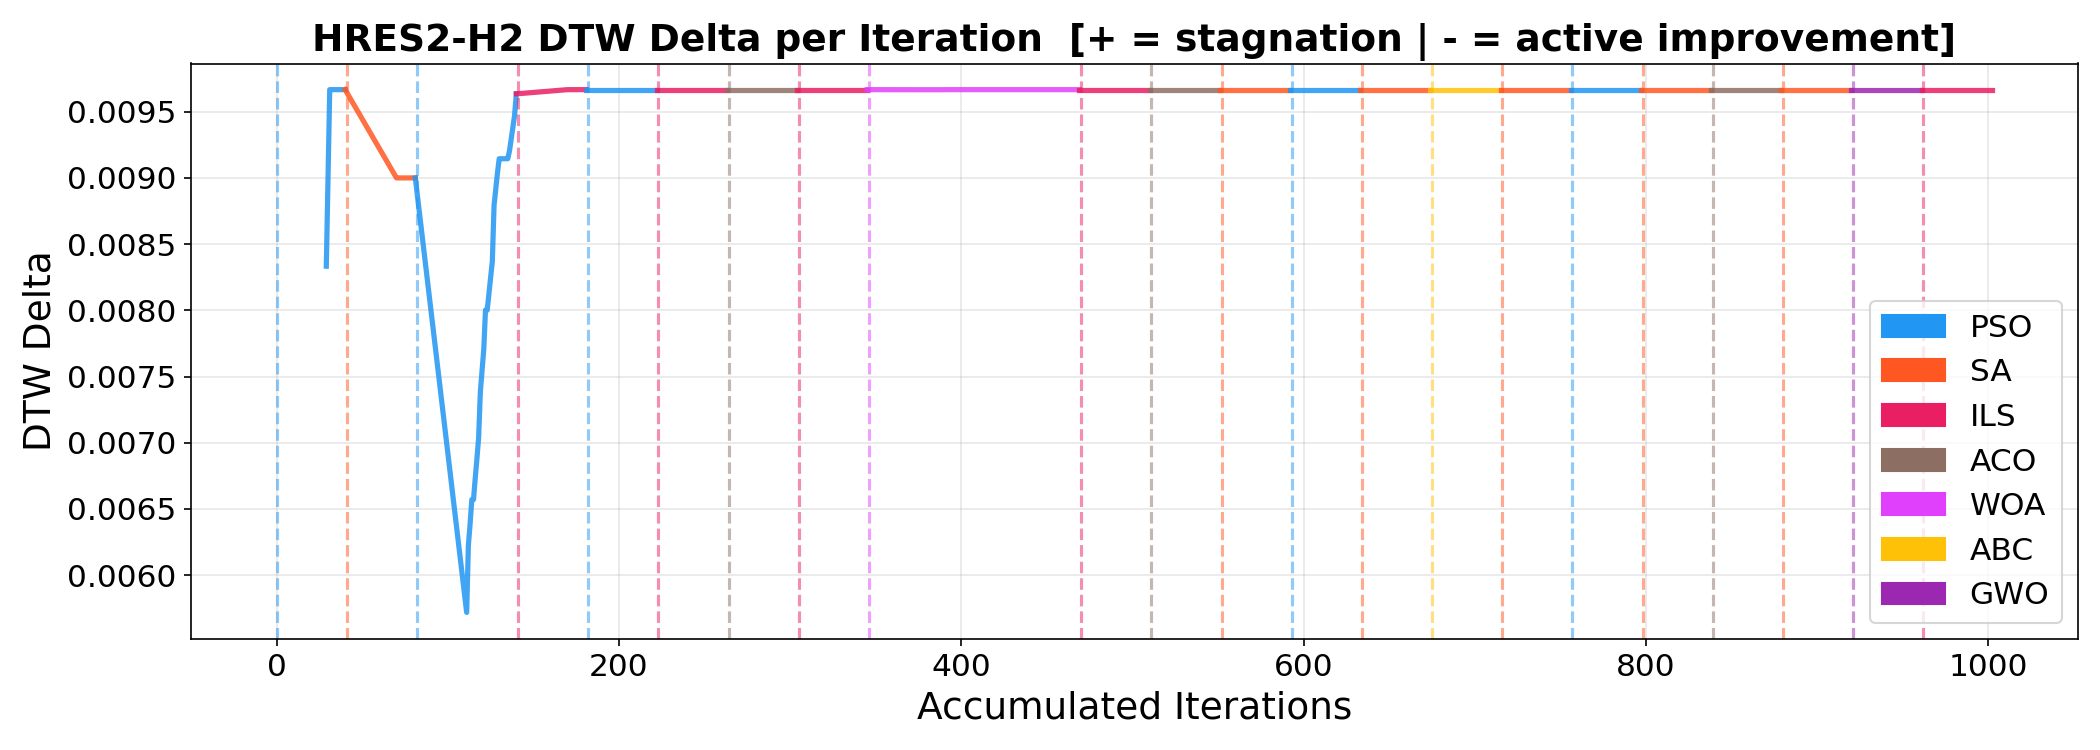
\includegraphics[width=0.85\textwidth]{imagenes_paper/hres2_ddtw_delta.png}
\caption{DDTW Framework derivative-based divergence metric profile ($\Delta = D_1 - D_2$) on HRES2-H2, evaluating rate-of-change signatures to initiate rotational handoffs.}
\label{fig:hres2_ddtw_delta}
\end{figure}

As shown in Figures~\ref{fig:hres2_dtw_conv} and
\ref{fig:hres2_ddtw_conv}, both modalities exhibit rapid initial descent
during the exploratory swarm phase ($t < 150$), followed by characteristic
convergence plateaus where standalone metaheuristics typically stall. In
Figure~\ref{fig:hres2_dtw_delta}, the DTW metric $\Delta$ tracks the
divergence between the sliding fitness window and synthetic reference
baselines, triggering rotational solver switches when stagnation is detected.
Similarly, Figure~\ref{fig:hres2_ddtw_delta} illustrates how the derivative-
based DDTW monitor detects slope flattening and initiates transitions between
global exploration and local exploitation. The final value should be
interpreted as the best observed solution on the fixed scenario, rather than as
a proof of global optimality.
